% =============================================================================
% EpiForecast-MX — Avance 6: Conclusiones Clave
% Equipo 01 — Maestría en Inteligencia Artificial Aplicada (MNA)
% Tecnológico de Monterrey x Instituto Mexicano del Seguro Social
% =============================================================================
\documentclass[12pt, letterpaper]{article}

% -- Paquetes ----------------------------------------------------------------
\usepackage[utf8]{inputenc}
\usepackage[T1]{fontenc}
\usepackage{lmodern}        % Latin Modern: soporta tamaños arbitrarios (70pt, 26pt, etc.)
\usepackage[spanish,es-tabla]{babel}
\usepackage{geometry}
\geometry{letterpaper, margin=2.5cm, top=3cm, bottom=2.5cm}
\setlength{\headheight}{14pt}
\setlength{\emergencystretch}{3em}  % Previene overfull hbox en párrafos con URLs/texttt largos
\usepackage{graphicx}
\graphicspath{{FigurasConclu/}{FigurasTableau/}}
\usepackage{float}
\usepackage{booktabs}
\usepackage{tabularx}
\usepackage{longtable}
\usepackage{multirow}
\usepackage{xcolor}
\usepackage{colortbl}
\usepackage{fancyhdr}
\usepackage{titlesec}
\usepackage{enumitem}
\usepackage{amsmath, amssymb}
\usepackage{caption}
\usepackage{subcaption}
\usepackage[most]{tcolorbox}
\usepackage{fontawesome5}
\usepackage{pifont}
\usepackage{parskip}
\usepackage{setspace}
\usepackage{array}
\usepackage[bottom]{footmisc}
\usepackage{xurl}
\usepackage[breaklinks=true]{hyperref}
\usepackage{tikz}
\usetikzlibrary{arrows.meta, positioning, shapes.geometric, fit, calc, decorations.pathreplacing, shadows.blur, colorbrewer, babel}
\usepackage{wrapfig}
\usepackage{pdflscape}
\usepackage{multicol}

% -- Colores institucionales IMSS / EpiForecast ------------------------------
\definecolor{burgundy}{HTML}{9B2242}
\definecolor{darkburgundy}{HTML}{6F1D46}
\definecolor{teal}{HTML}{00524E}
\definecolor{darkteal}{HTML}{173F35}
\definecolor{gold}{HTML}{B58500}
\definecolor{coolgray}{HTML}{97999B}
\definecolor{imssblue}{HTML}{003A70}
\definecolor{cream}{HTML}{F5EDE0}
\definecolor{lightgreen}{HTML}{E6F4EA}
\definecolor{lightyellow}{HTML}{FEF7E0}
\definecolor{lightred}{HTML}{FDE8E8}
% Off-palette (ERD y diagramas Tableau)
\definecolor{slateborder}{HTML}{4A5568}
\definecolor{slatelight}{HTML}{EDF2F7}
\definecolor{burntborder}{HTML}{C05621}
\definecolor{burntlight}{HTML}{FEEBC8}

% Colores específicos por Motor MLOps
\definecolor{cprophet}{HTML}{004D40}
\definecolor{cdeepar}{HTML}{880E4F}
\definecolor{censemble}{HTML}{FF6F00}
\definecolor{cstacking}{HTML}{1A237E}

% Colores profesionales para diagramas SOLID
\definecolor{solidblue}{RGB}{41, 128, 185}
\definecolor{solidgreen}{RGB}{39, 174, 96}
\definecolor{solidorange}{RGB}{211, 84, 0}
\definecolor{solidpurple}{RGB}{142, 68, 173}
\definecolor{solidred}{RGB}{192, 57, 43}

% -- Configuración de hyperref -----------------------------------------------
\hypersetup{
    colorlinks=true,
    linkcolor=teal,
    citecolor=burgundy,
    urlcolor=imssblue,
    bookmarksopen=true,
    pdftitle={EpiForecast-MX | Avance 6: Conclusiones Clave},
    pdfauthor={Equipo 01 | MNA Tec de Monterrey},
}

% -- Pies de foto centrados y en gris ----------------------------------------
\captionsetup{
    font={small, color=coolgray},
    labelfont={bf, color=coolgray},
    justification=centering
}
% Se comenta para evitar advertencia de 'unused' si no hay subfigures en el paso actual
% \captionsetup[subfigure]{ ... }

% -- Headers y footers -------------------------------------------------------
\pagestyle{fancy}
\fancyhf{}
\fancyhead[L]{\small\textcolor{coolgray}{EpiForecast-MX | Avance 6: Conclusiones Clave}}
\fancyhead[R]{\small\textcolor{coolgray}{Equipo 01 | MNA | Tec de Monterrey}}
\fancyfoot[C]{\thepage}
\fancyfoot[R]{\small\textcolor{coolgray}{Marzo 2026}}
\renewcommand{\headrulewidth}{0.4pt}
\renewcommand{\footrulewidth}{0.2pt}

% -- Títulos con colores IMSS ------------------------------------------------
\titleformat{\section}
  {\Large\bfseries\color{teal}}{\thesection.}{0.5em}{}[\vspace{-0.5em}\textcolor{teal}{\rule{\textwidth}{1pt}}]
\titleformat{\subsection}
  {\large\bfseries\color{burgundy}}{\thesubsection}{0.5em}{}
\titleformat{\subsubsection}
  {\normalsize\bfseries\color{darkteal}}{\thesubsubsection}{0.5em}{}

% -- Cajas de callout --------------------------------------------------------
\newtcolorbox{insightbox}[1][]{
  colback=lightgreen, colframe=teal,
  boxrule=0pt, leftrule=4pt, arc=2pt,
  fonttitle=\bfseries, title=#1,
  before upper={\setlength{\emergencystretch}{5em}}
}
\newtcolorbox{warningbox}[1][]{
  colback=lightyellow, colframe=gold,
  boxrule=0pt, leftrule=4pt, arc=2pt,
  fonttitle=\bfseries, title=#1,
  before upper={\setlength{\emergencystretch}{5em}}
}
\newtcolorbox{criticalbox}[1][]{
  colback=lightred, colframe=burgundy,
  boxrule=0pt, leftrule=4pt, arc=2pt,
  fonttitle=\bfseries, title=#1,
  before upper={\setlength{\emergencystretch}{5em}}
}

% Caja de Campeón en Producción (Dorada)
\newtcolorbox{championbox}[1][]{
  colback=white, colframe=gold,
  boxrule=2pt, arc=6pt,
  fonttitle=\bfseries\large, coltitle=black,
  title={\textcolor{gold}{\faTrophy}\ \textbf{Modelo Campeón en Producción} #1}
}

% -- Comandos personalizados (Robustos para evitar error de fuente) ----------
\newcommand{\smape}{\textnormal{\textsc{smape}}}
\newcommand{\mase}{\textnormal{\textsc{mase}}}
\newcommand{\rmse}{\textnormal{\textsc{rmse}}}
\newcommand{\mae}{\textnormal{\textsc{mae}}}
\newcommand{\mape}{\textnormal{\textsc{mape}}}
\newcommand{\imss}{\textnormal{\textsc{imss}}}
\newcommand{\tabref}[1]{Tabla~\ref{#1}}
\newcommand{\figref}[1]{Figura~\ref{#1}}
\newcommand{\secref}[1]{Sección~\ref{#1}}

% -- Separador visual --------------------------------------------------------
\newcommand{\sepsection}{\vspace{0.5cm}\noindent\textcolor{coolgray}{\rule{\textwidth}{0.3pt}}\vspace{0.3cm}}

% -- ERD styles (diagramas Tableau) ------------------------------------------
\pgfdeclarelayer{background}
\pgfsetlayers{background,main}
\newlength{\rowh}  \setlength{\rowh}{0.52cm}
\newlength{\tabw}  \setlength{\tabw}{5.4cm}
\newlength{\hdrh}  \setlength{\hdrh}{0.62cm}
\tikzset{
  dbheader/.style={rectangle, draw=#1, fill=#1,
    minimum width=\tabw, minimum height=\hdrh, anchor=north, align=center,
    font=\sffamily\bfseries\small\color{white}, inner sep=0pt},
  dbkeyrow/.style={rectangle, draw=#1!30, fill=#1!06,
    minimum width=\tabw, minimum height=\rowh,
    text width=\dimexpr\tabw-12pt\relax,
    anchor=north, align=left, font=\sffamily\small\bfseries\color{#1},
    inner xsep=6pt, inner ysep=0pt},
  dbdatarow/.style={rectangle, draw=coolgray!25, fill=white,
    minimum width=\tabw, minimum height=\rowh,
    text width=\dimexpr\tabw-12pt\relax,
    anchor=north, align=left, font=\sffamily\small\color{black!70},
    inner xsep=6pt, inner ysep=0pt},
  conn/.style={draw=coolgray, thick, shorten >=2pt, shorten <=2pt},
  joinlabel/.style={rectangle, fill=white, draw=coolgray!40,
    font=\sffamily\scriptsize\color{coolgray!80},
    inner sep=3pt, rounded corners=2pt},
}
\newcommand{\erdpk}{\textcolor{gold}{\textbf{[PK]}}}
\newcommand{\erdfk}{\textcolor{imssblue}{\textbf{[FK]}}}
\newcommand{\keyicon}{{\small$\bullet$}\ }
\newcommand{\dataicon}{{\small\textcolor{coolgray}{$\circ$}}\ }

% =============================================================================
% INVENTARIO DE IMAGENES ESPERADAS (subir todas a FigurasConclu/ en Overleaf)
% =============================================================================
% OBLIGATORIAS (portada / reflexiones):
%   logo_tec.png                         — Logo Tec de Monterrey
%   logo_imss.png                        — Logo IMSS
%   JARS2026.jpg                         — Foto Javier
%   JARCOS2026.jpg                       — Foto Juan Carlos
%   LUIS2026.jpg                         — Foto Luis
%
% FIGURAS DE DATOS (generadas con matplotlib/seaborn/geopandas):
%   fig_distribucion_motores.png         — Donut chart motores ganadores
%   fig_mapa_regiones_inegi.png          — Mapa coroplético 4 regiones de salud mental
%   fig_forecast_depresion_nacional.png  — Real vs DeepAR Depresión Nacional
%   fig_forecast_parkinson_nacional.png  — Real vs DeepAR Parkinson Nacional
%   fig_forecast_alzheimer_nacional.png  — Real vs DeepAR Alzheimer Nacional
%   fig_mapa_smape_depresion.png         — Mapa semáforo SMAPE por estado
%   fig_boxplot_smape_motores.png        — Box plot SMAPE por motor/padecimiento
%   fig_barras_mase_motores.png          — % series con MASE < 1 por motor
%   fig_distribucion_sexo.png            — Stacked bar incidencia por sexo
%   fig_covid_impact_depresion.png       — Timeline Depresión con zona COVID
%   fig_radar_cloud_providers.png        — Radar chart 4 proveedores cloud
%   fig_heatmap_smape_estado_pad.png     — Heatmap SMAPE estados × padecimiento
%   fig_tendencia_3_padecimientos.png    — 3 series nacionales superpuestas
%   fig_tendencia_3_5_cortes.png         — Composición visual 333 series (5 cortes)
%   fig_costos_aws_12m.png               — Gráfico costos AWS 12 meses
%
% SCREENSHOTS / EVIDENCIAS MLOPS:
%   screenshot_validacion_semanal.png    — Reporte HTML validación semanal
%   fig_github_actions_ci.png            — Pipeline CI/CD verde en GitHub
%   fig_test_coverage.png                — Reporte cobertura pytest
%   fig_epiconsole_help.png              — Terminal con make help (EPI Console)
%   fig_ruff_lint_clean.png              — Terminal con ruff check sin errores
%   fig_mypy_clean.png                   — Terminal con mypy sin errores
%   fig_precommit_pass.png               — Terminal con pre-commit hooks pasando
%   fig_dvc_dag.png                      — DAG de DVC (dvc dag output)
%   fig_s3_bucket_structure.png          — Consola AWS S3 con estructura de datos
%   fig_sagemaker_training.png           — Consola SageMaker training job
%   fig_sagemaker_gpu_metrics.png        — CloudWatch GPU utilization
%   fig_docker_build.png                 — Terminal con Docker build exitoso
%   fig_ecr_repository.png               — Consola ECR con imagen publicada
%   fig_github_tags.png                  — Historial de tags semánticos en GitHub
%   04_CookieCutterRepo.png              — Estructura arquitectura Cookiecutter
%   PropuestaDeployments.png             — Calendario de operaciones
%   estrategia_monitoreo.png             — Diagrama 3 pilares monitoreo
%   fig_dashboard_tableau.png            — Dashboard Tableau
%   01_TableauDashboard_AcumuladoCasosPorAnio.png — Tableau: casos acumulados por año
%   02_TableauDashboard_PrediccionZoomY52SemanasPreviasYFuturas.png — Tableau: predicción + zoom 52 sem
%   03_TableauDashboardTableroDeModelos.png — Tableau: tablero general de 333 modelos
%   fig_website_proyecto.png             — Landing page proyectointegrador.org
%   fig_equipo_foto.png                  — Foto grupal del equipo (opcional)
%   fig_github_repo_overview.png         — Página principal del repo en GitHub
%   fig_github_pr_review.png             — Pull request con code review
% =============================================================================

\begin{document}
\shorthandoff{<>}

% =============================================================================
% PORTADA
% =============================================================================
\begin{titlepage}
\begin{center}

\vspace*{0.5cm}


\includegraphics[height=2cm]{logo_tec.png}\hspace{2cm}
\includegraphics[height=2.5cm]{logo_imss.png}

\vspace{0.5cm}

{\small Instituto Tecnológico y de Estudios Superiores de Monterrey}\\[0.1cm]
{\small Maestría en Inteligencia Artificial Aplicada (MNA)}\\[0.5cm]

\textcolor{teal}{\rule{\textwidth}{2pt}}\\[0.4cm]
{\Huge\bfseries\textcolor{teal}{EpiForecast-MX}}\\[0.2cm]
{\LARGE\textcolor{burgundy}{Avance 6: Conclusiones Clave}}\\[0.3cm]
\textcolor{teal}{\rule{\textwidth}{2pt}}\\[0.8cm]

{\large\textit{Generalización de modelos nacionales de pronóstico\\
epidemiológico hacia un enfoque modular con desagregación\\
por sexo y entidad federativa en México}}\\[1.2cm]

{\large\textbf{Materia:} Proyecto Integrador | TC5035.10}\\[0.5cm]

\begin{tabular}{ll}
\textbf{Asesora:}     & Dra.\ Grettel Barceló Alonso \\
\textbf{Director MNA:}& Dr.\ Luis Eduardo Falcón Morales \\
\textbf{Profesora:}   & Mtra.\ Verónica Sandra Guzmán de Valle \\
\textbf{IMSS:}        & Dra.\ Ruth Pérez-Hernández (Líder de Proyecto) \\
                      & Dra.\ Lina Díaz Castro (Investigadora en Psiquiatría) \\
\end{tabular}\\[1cm]

\textbf{\Large Equipo 01}\\[0.4cm]
% IMAGEN OPCIONAL: Foto grupal del equipo
% \includegraphics[width=8cm]{fig_equipo_foto.png}\\[0.3cm]
\begin{tabular}{lll}
\textbf{Javier A. Rebull Saucedo} & A01795838 & Sr.\ Assoc.\ Dev., Santander Bank US \\
\textbf{Juan Carlos Pérez Nava}   & A01795941 & Head of Area, IMSS \\
\textbf{Luis G. Sánchez Salazar}  & A01232963 & Sr.\ Controls Engineer, Tesla \\
\end{tabular}\\[1.0cm]

{\large Semana 8, Marzo 2026}

\end{center}
\end{titlepage}

% =============================================================================
% TABLA DE CONTENIDOS
% =============================================================================
\newpage
\tableofcontents
\newpage
\listoffigures
\listoftables
\newpage


% =============================================================================
% ABSTRACT — Una sola página
% =============================================================================
\newpage
\section*{Abstract}\label{sec:abstract}
\addcontentsline{toc}{section}{Abstract}

La vigilancia epidemiológica en México enfrenta una presión creciente: anticipar, con tiempo y detalle, la demanda de atención en salud mental y neurología dentro de un sistema que atiende a más de 80 millones de derechohabientes. Sin embargo, la planeación institucional suele apoyarse en promedios históricos que \emph{miran al pasado}, sin alertar a tiempo sobre cambios de tendencia, diferencias entre estados o impactos extraordinarios como la pandemia de COVID-19. El resultado puede traducirse en decisiones tardías en la distribución de medicamentos, la disponibilidad de especialistas y la preparación hospitalaria.

Este trabajo presenta las conclusiones clave de \textbf{EpiForecast-MX}, una plataforma inteligente de pronóstico epidemiológico diseñada para responder una pregunta clínicamente útil: \textit{¿cuántos casos de cada padecimiento se esperan la próxima semana en cada estado y para cada sexo?}
Estos motores de IA se aplican a tres padecimientos de la Clasificación Internacional de Enfermedades: \textbf{Depresión (F32)}, \textbf{Parkinson (G20)} y \textbf{Alzheimer (G30)}, cubriendo las 32 entidades federativas, 4 regiones de salud mental y el nivel nacional, con desagregación por sexo y un horizonte de 52 semanas. En total, el sistema opera \textbf{333 modelos de producción}, evaluados con dos métricas estándar: \smape{} (error porcentual simétrico; menor es mejor) y \mase{} (error comparado contra una predicción simple que repite el año anterior; valores menores a 1 indican superioridad del modelo).

Los resultados muestran que \textbf{DeepAR} es el motor de IA más preciso, ganando el 73.3\% de las 333 series. El sistema de selección automática alcanza un \smape{} mediano de producción de 23.66\% y un \mase{} de 0.30 (solo el 30\% del error de la predicción ingenua). \textbf{Depresión} es el padecimiento mejor pronosticado (\smape{} mediano 5.99\%), mientras que \textbf{Parkinson} (35.24\%) y \textbf{Alzheimer} (107.59\%) exhiben errores porcentuales más altos por su \emph{baja incidencia absoluta} (menos de 5 casos semanales en muchos estados), no por fallas del modelo; en términos clínicos, el error promedio en Alzheimer es menor a 1 caso por semana. La infraestructura tecnológica respalda la reproducibilidad mediante 855 pruebas automatizadas y entrenamiento en la nube de Amazon (AWS SageMaker) con un costo de entrenamiento GPU de \$3.50\,--\,\$8.50~USD por job y un costo operativo total de \$4.40\,--\,\$9.40~USD por corrida, incluyendo almacenamiento y servicios auxiliares (véase Apéndice~\ref{sec:logs_sagemaker}).

\textbf{EpiForecast-MX} demuestra que es viable construir un sistema de pronóstico epidemiológico basado en inteligencia artificial, escalable y económicamente accesible para una institución pública de salud, generando información \emph{accionable} para anticiparse en la toma de decisiones clínicas y administrativas en México.

\vspace{0.8cm}

\noindent\textbf{Palabras clave:} pronóstico epidemiológico, series de tiempo, inteligencia artificial, DeepAR, Prophet, ensemble learning, salud mental, depresión, Parkinson, Alzheimer, IMSS, MLOps, AWS SageMaker, vigilancia epidemiológica, México.

\newpage


% =============================================================================
% PÁGINA DE CITA — George E. P. Box (Versión Elegante)
% =============================================================================
\newpage
\thispagestyle{empty}
\vspace*{\fill}

\begin{center}

% 1. Comilla superior gigante pero sutil (actúa casi como marca de agua)
{\color{teal!40}\fontsize{70}{70}\selectfont \faQuoteLeft}

\vspace{0.8cm}

% 2. La cita agrupada en un solo bloque para mejor cohesión
\begin{minipage}{0.75\textwidth}
    \centering
    {\fontsize{26}{36}\selectfont\itshape\textcolor{darkteal}{%
    All models are wrong,\\[0.5em]
    but some are useful.}}
\end{minipage}

\vspace{1.5cm}

% 3. Separador clásico: línea muy fina con un pequeño rombo central
\begin{tikzpicture}
  \draw[burgundy, line width=0.4pt] (-3.5, 0) -- (3.5, 0);
  \fill[burgundy] (0,0) ++(0, 3pt) -- ++(3pt, -3pt) -- ++(-3pt, -3pt) -- ++(-3pt, 3pt) -- cycle;
\end{tikzpicture}

\vspace{1cm}

% 4. Autor con espaciado amplio y elegante
{\Large\textsc{\textcolor{burgundy}{George E. P. Box}}}

\vspace{0.4cm}

% 5. Referencia bibliográfica delicada
{\small\textcolor{coolgray}{\textit{Robustness in the Strategy of Scientific Model Building}, 1979}}

\end{center}

\vspace*{\fill}

\newpage
% =============================================================================
% 1. RESUMEN EJECUTIVO
% =============================================================================
\section{Resumen Ejecutivo}\label{sec:resumen}

Este documento consolida las conclusiones del proyecto EpiForecast-MX tras completar el ciclo de modelado, evaluación y validación con datos reales. A continuación se sintetizan los hallazgos, las decisiones de producción y las recomendaciones operativas dirigidas a los stakeholders del IMSS.

\subsection{Hallazgos principales}

Tras evaluar \textbf{1,332 combinaciones} (4 motores $\times$ 333 series), los resultados clave son (véase la \figref{fig:donut_motores} para la distribución de motores ganadores):

\begin{enumerate}[noitemsep]
    \item \textbf{DeepAR domina la producción}: ganó 244 de 333 series (73.3\%), seguido de Prophet (55, 16.5\%), Ensemble (32, 9.6\%) y Stacking (2, 0.6\%), como ilustra la \figref{fig:donut_motores}. La selección se realiza \textit{serie por serie} con base en el \smape{} de validación cruzada; las 89 series restantes fueron asignadas a otros motores por presentar mejor ajuste individual. La superioridad general de DeepAR radica en su capacidad para capturar patrones no lineales y cross-learning entre series, tal como describen Salinas et al.\ (2020).
    \item \textbf{Depresión es el padecimiento mejor modelado}: \smape{} medio de 7.38\% y mediano de 5.99\%, con \mase{} medio de 0.25 que supera al naive estacional lag-52 en un 75\%.
    \item \textbf{Padecimientos raros presentan un reto inherente}: Parkinson (\smape{} mediano 35.24\%) y Alzheimer (\smape{} mediano 107.59\%) muestran errores elevados debido a la baja incidencia ($<$5 casos/semana en muchos estados), no a fallos del modelo. Hyndman y Koehler (2006) advierten que las métricas porcentuales se distorsionan con valores cercanos a cero.
    \item \textbf{Infraestructura de grado producción}: 855 tests (849 unitarias, 3 de integración y 3 lentas), cobertura del 92\%, CI/CD con GitHub Actions, DVC para versionado y un pipeline reproducible de más de 50 comandos Make.
    \item \textbf{Costo validado en la nube}: el entrenamiento completo de DeepAR en GPU (ml.g4dn.xlarge) costó \$3.50\,--\,\$8.50 USD por job de entrenamiento (rango observado en tres ejecuciones reales en AWS; véase Apéndice~\ref{sec:logs_sagemaker}), con un costo operativo anual proyectado de \$240\,--\,\$506 USD.
\end{enumerate}

% IMAGEN: Donut chart con distribución de motores ganadores
\begin{figure}[H]
\centering
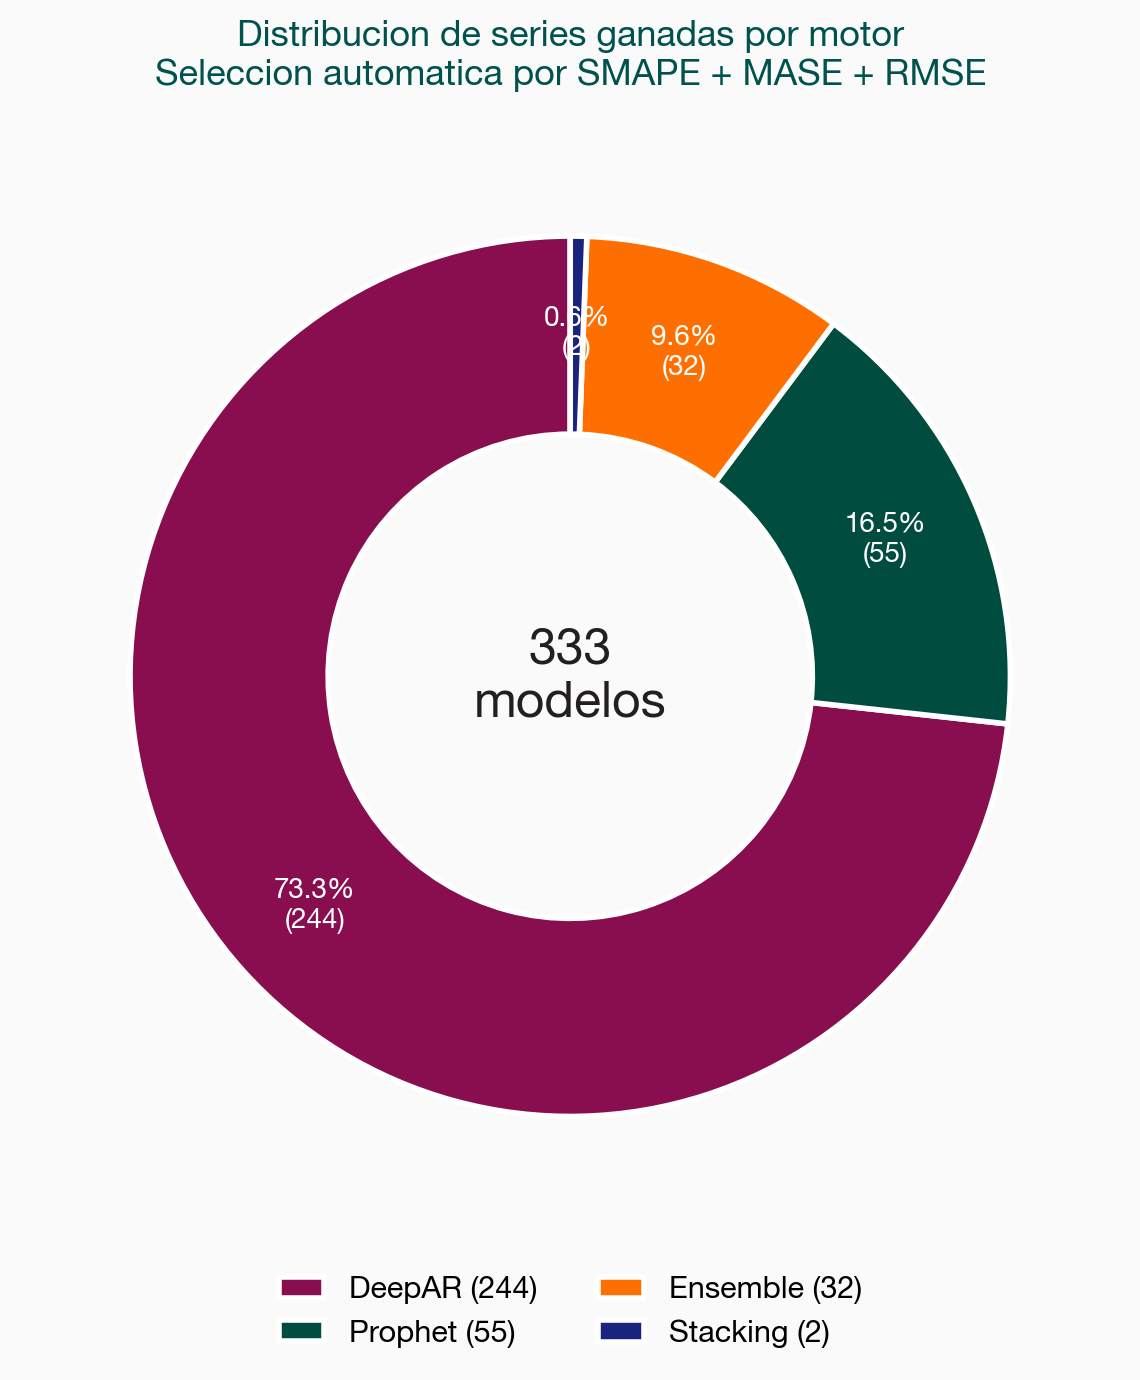
\includegraphics[width=0.65\textwidth]{fig_distribucion_motores.png}
\caption[Distribución de series ganadas por motor.]{Distribución de series ganadas por motor de pronóstico (333 series de producción). DeepAR domina con el 73.3\% de las series.}
\label{fig:donut_motores}
\end{figure}

\newpage

\subsection{Decisiones de producción}

Las siguientes decisiones se derivan directamente de los resultados de evaluación y condicionan la operación del sistema:

\begin{table}[H]
\centering
\caption{Decisiones de producción derivadas de la evaluación}
\label{tab:decisiones_prod}
\small
\begin{tabularx}{\textwidth}{>{\bfseries}l X}
\toprule
\textbf{Decisión} & \textbf{Justificación} \\
\midrule
Motor primario: DeepAR & Gana 73.3\% de series; cross-learning mitiga datos escasos por estado \\
Métrica de selección: \smape{} & Primario, con \mase{} como desempate (umbral 5\%) y \rmse{} como segundo desempate \\
Reentrenamiento trimestral & Series de cambio lento; 92\% de ahorro en entrenamiento GPU vs.\ semanal sin degradación significativa esperada en la precisión \\
Fallback regional & 8 series con incidencia insuficiente usan el modelo de su región de salud mental \\
Proveedor cloud: AWS & Puntuación ponderada 9.3/10; costo validado y ecosistema maduro \\
\bottomrule
\end{tabularx}
\end{table}

\subsection{Recomendación de despliegue}

Se recomienda desplegar EpiForecast-MX en \textbf{AWS SageMaker} como proveedor primario, con un ciclo operativo de dos capas:

\begin{itemize}[noitemsep]
    \item \textbf{Ciclo semanal} (ligero): descarga de boletín SINAVE, inferencia batch con modelos vigentes, actualización de dashboard Tableau y validación automática pronóstico vs.\ realidad.
    \item \textbf{Ciclo trimestral} (pesado): reentrenamiento completo de 333 modelos en GPU, validación cruzada, diagnóstico de overfitting y promoción a producción con aprobación del epidemiólogo.
\end{itemize}

El costo proyectado es de \$60\,--\,\$127 USD/trimestre (\$240\,--\,\$506 USD/año), equivalente al costo de 7\,--\,15 consultas de neurología.\footnote{Costo estimado de consulta de neurología en el sector privado mexicano: \$34\,--\,\$72 USD (rango de mercado, 2025). El IMSS no publica tabuladores individuales por especialidad; la cifra se usa como referencia comparativa, no como dato institucional.}

\newpage
% =============================================================================
% 2. INTRODUCCION Y CONTEXTO
% =============================================================================
\section{Introducción y Contexto}\label{sec:introduccion}

\subsection{El problema epidemiológico}

El {\imss} atiende a más de 80 millones de derechohabientes y enfrenta el reto de planificar recursos médicos para padecimientos de salud mental y neurológicos cuya incidencia varía significativamente por región, estacionalidad y dinámicas demográficas. Actualmente, la planificación se basa en promedios históricos, sin capacidad de anticipar cambios de tendencia ni impactos exógenos como la pandemia de COVID-19. Miller (2022) destaca que la toma de decisiones basada en datos mejora significativamente los resultados en la gestión de proyectos institucionales.

EpiForecast-MX aborda este reto desarrollando modelos de pronóstico para tres padecimientos de la Clasificación Internacional de Enfermedades, 10.ª revisión (CIE-10):

\begin{itemize}[noitemsep]
    \item \textbf{Trastorno depresivo (F32)}: el de mayor incidencia y variabilidad. Fuertemente impactado por COVID-19, con un aumento sostenido post-pandemia. La Organización Mundial de la Salud (OMS, s.\,f.) lo identifica como una de las principales causas de discapacidad a nivel global.
    \item \textbf{Enfermedad de Parkinson (G20)}: baja incidencia con patrones regulares y estacionalidad suave.
    \item \textbf{Enfermedad de Alzheimer (G30)}: incidencia muy baja y estable; la más predecible en términos absolutos pero la más difícil en error porcentual.
\end{itemize}

Como se evidencia en la \figref{fig:tendencia_3pad}, la disparidad de volumen entre los padecimientos condiciona la precisión relativa de los modelos:

\begin{figure}[H]
\centering
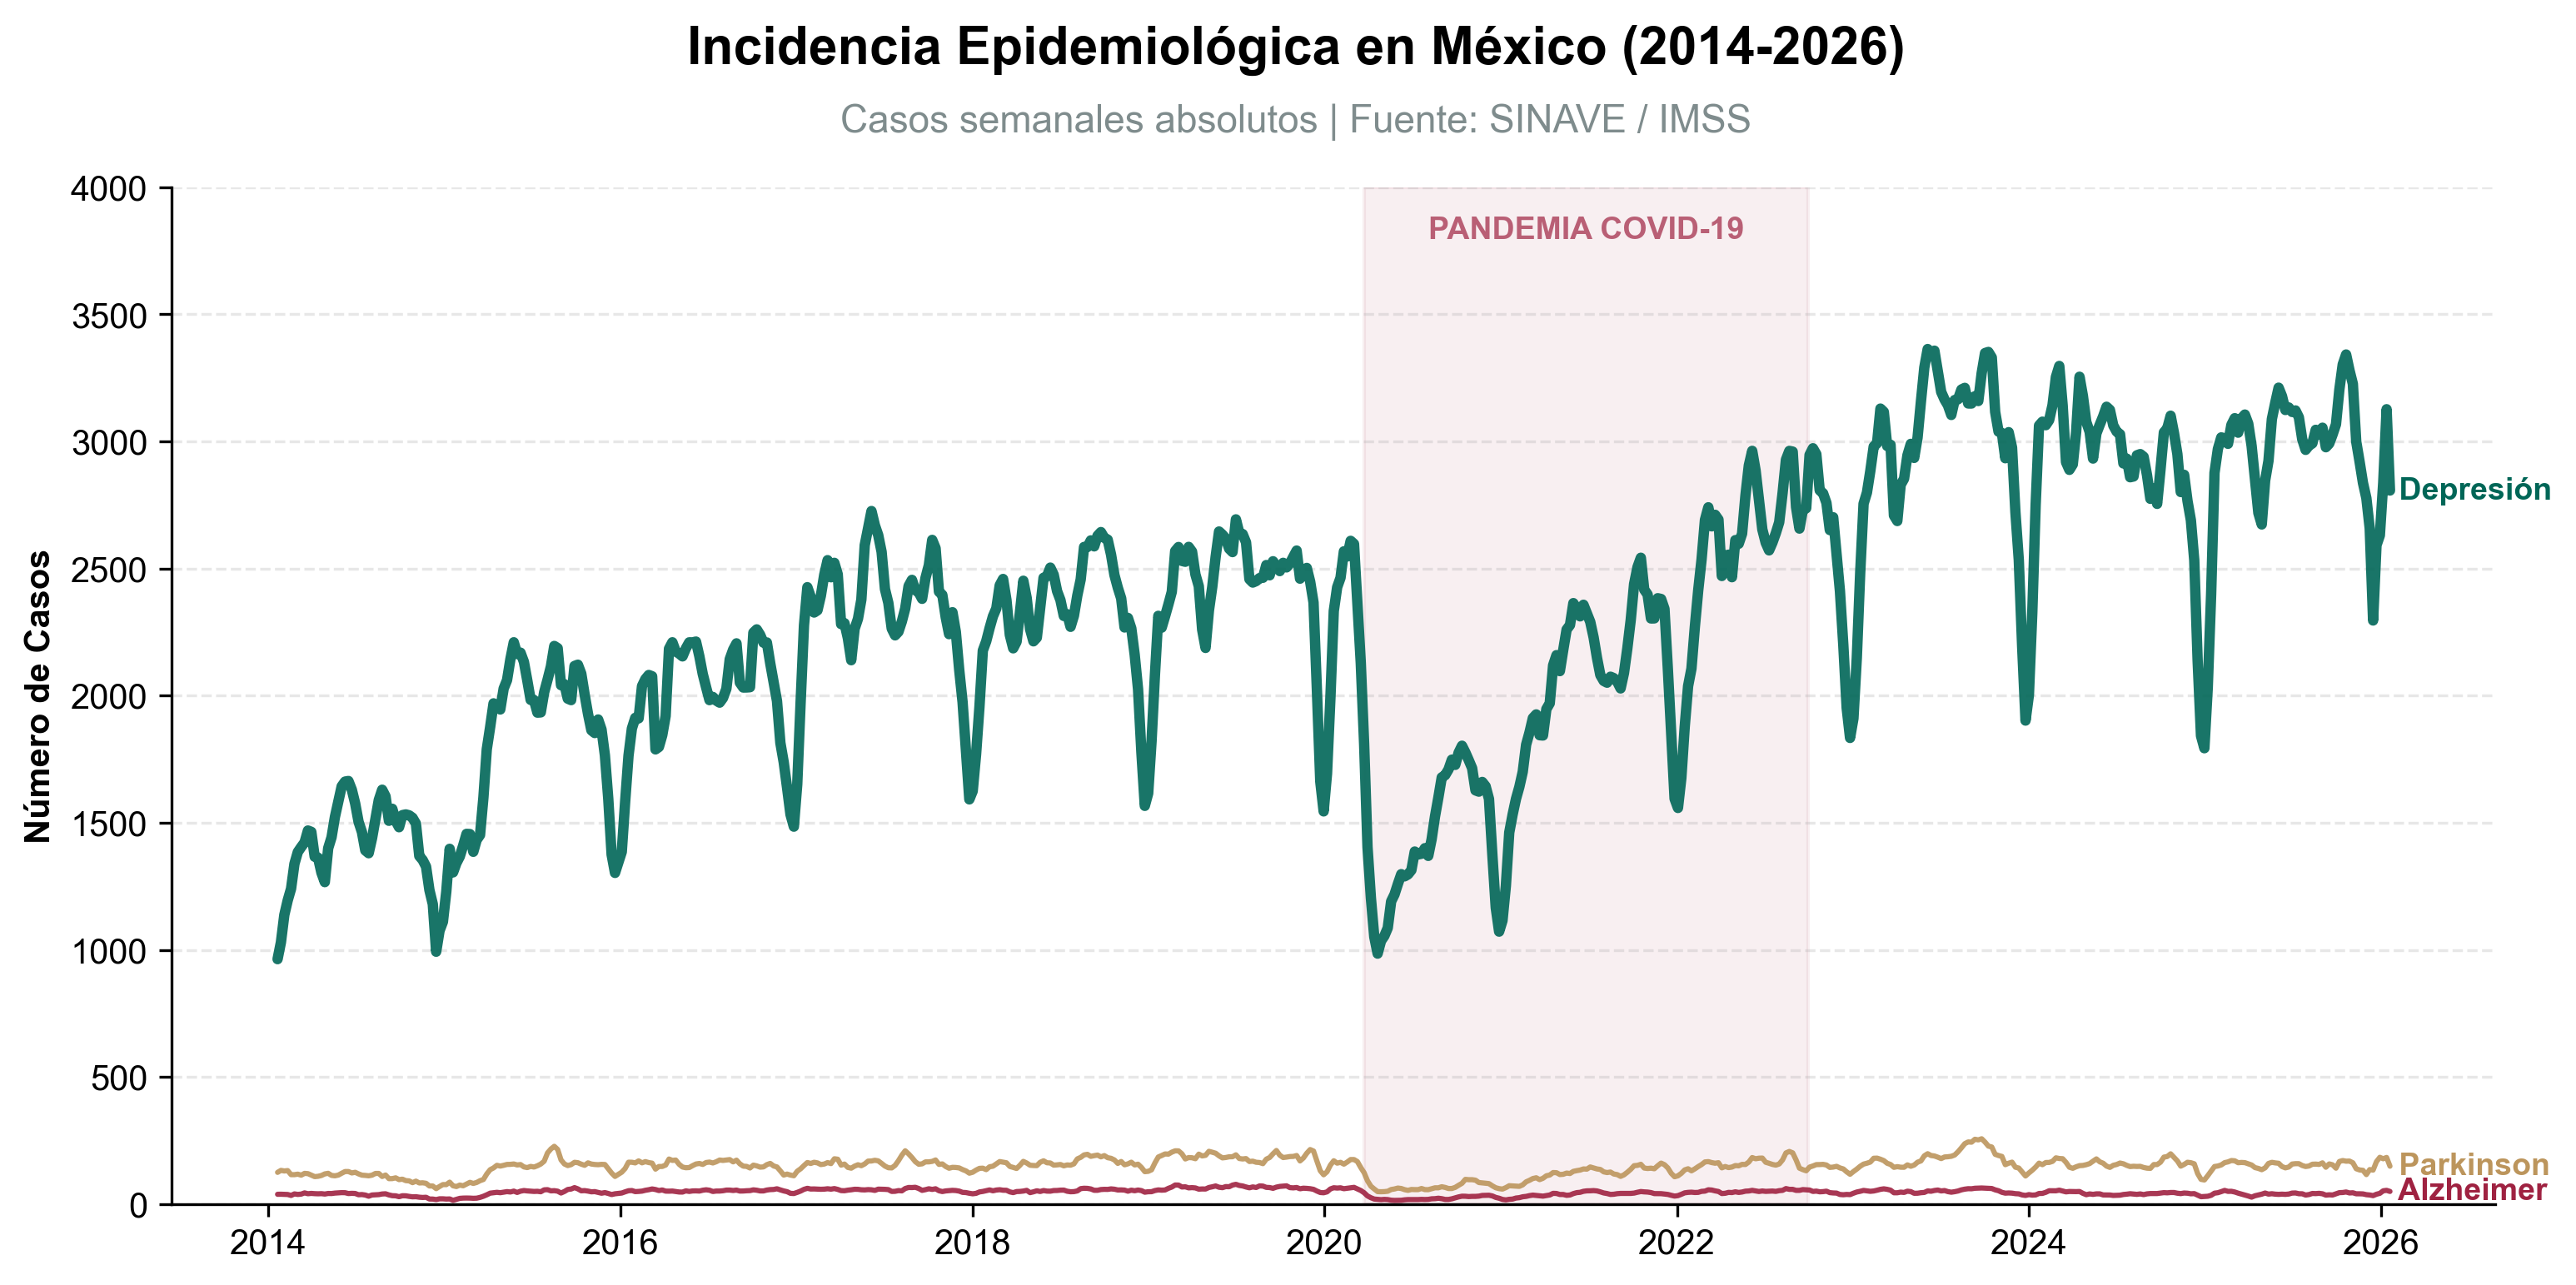
\includegraphics[width=0.95\textwidth]{fig_tendencia_3_padecimientos.png}
\caption[Tendencia histórica nacional.]{Incidencia semanal nacional de los tres padecimientos (2014--2026). Depresión (F32) presenta un orden de magnitud mayor que Parkinson (G20) y Alzheimer (G30).}
\label{fig:tendencia_3pad}
\end{figure}

\subsection{Vinculación con criterios del Avance 0}

Este documento de conclusiones responde directamente a los tres ejes de evaluación establecidos en el Avance 0:

\begin{enumerate}[noitemsep]
    \item \textbf{Análisis del modelo}: \secref{sec:rendimiento} presenta métricas detalladas (\smape{}, \mase{}, \rmse{}, \mae{}) para los 1,332 modelos evaluados, con diagnósticos de overfitting y leakage.
    \item \textbf{Accionables por stakeholder}: \secref{sec:accionables} define una matriz de responsabilidad con acciones concretas para cada actor del ecosistema.
    \item \textbf{Análisis de implementación cloud}: \secref{sec:cloud} compara cuatro proveedores con una metodología de puntuación ponderada y presenta costos reales de producción.
\end{enumerate}

\newpage

\subsection{Definiciones fundamentales}

Para facilitar la lectura, se definen los términos técnicos de primera mención. Un glosario completo se encuentra en el Apéndice~\ref{sec:glosario}.

\begin{table}[H]
\centering
\caption{Definiciones de métricas y conceptos clave}
\label{tab:definiciones}
\small
\begin{tabularx}{\textwidth}{>{\bfseries}l X}
\toprule
\textbf{Término} & \textbf{Definición} \\
\midrule
\smape{} & Symmetric Mean Absolute Percentage Error. Mide el error porcentual simétrico entre predicción y realidad; rango $[0\%, 200\%]$. \\
\mase{} & Mean Absolute Scaled Error. Compara el error del modelo contra un naive estacional (lag-52); $<$1 indica superioridad (Hyndman \& Koehler, 2006). \\
\rmse{} & Root Mean Squared Error. Penaliza errores grandes; en las mismas unidades que la variable objetivo. \\
\mae{} & Mean Absolute Error. Error promedio absoluto; robusto a outliers. \\
CV & Cross-Validation. Validación cruzada temporal con ventanas expansivas que respetan la causalidad. \\
Prophet & Modelo aditivo que descompone series en tendencia, estacionalidad y regresores (Taylor \& Letham, 2018). \\
DeepAR & Red neuronal autoregresiva que aprende distribución probabilística multiserie (Salinas et al., 2020). \\
Ensemble & Combinación de Prophet (tendencia) + XGBoost (residuales) para capturar no linealidades (Chen \& Guestrin, 2016). \\
Stacking & Meta-aprendizaje donde Prophet, ETS y LightGBM (Ke et al., 2017) alimentan un meta-learner Ridge. \\
\bottomrule
\end{tabularx}
\end{table}

\newpage
% =============================================================================
% 3. COMPOSICION DE LAS 333 SERIES
% =============================================================================
\section{Composición de las 333 Series}\label{sec:composicion}

\subsection{Fórmula de composición}

El número de series de producción se obtiene mediante la combinatoria completa de tres dimensiones:

\begin{equation}\label{eq:333}
\underbrace{37}_{\text{geografías}} \;\times\; \underbrace{3}_{\text{padecimientos}} \;\times\; \underbrace{3}_{\substack{\text{cortes por tipo}}} \;=\; \mathbf{333} \text{ series}
\end{equation}

Los \textbf{3 cortes por tipo} corresponden a:
\begin{enumerate}[noitemsep]
    \item \textbf{Combinado (General)}: ambos sexos agregados.
    \item \textbf{Masculino}: solo casos del sexo masculino.
    \item \textbf{Femenino}: solo casos del sexo femenino.
\end{enumerate}

La \tabref{tab:composicion} desglosa cada nivel geográfico, y la \figref{fig:composicion_visual} ofrece una visualización integral de las tres dimensiones que componen el universo de modelos.

\begin{figure}[H]
\centering
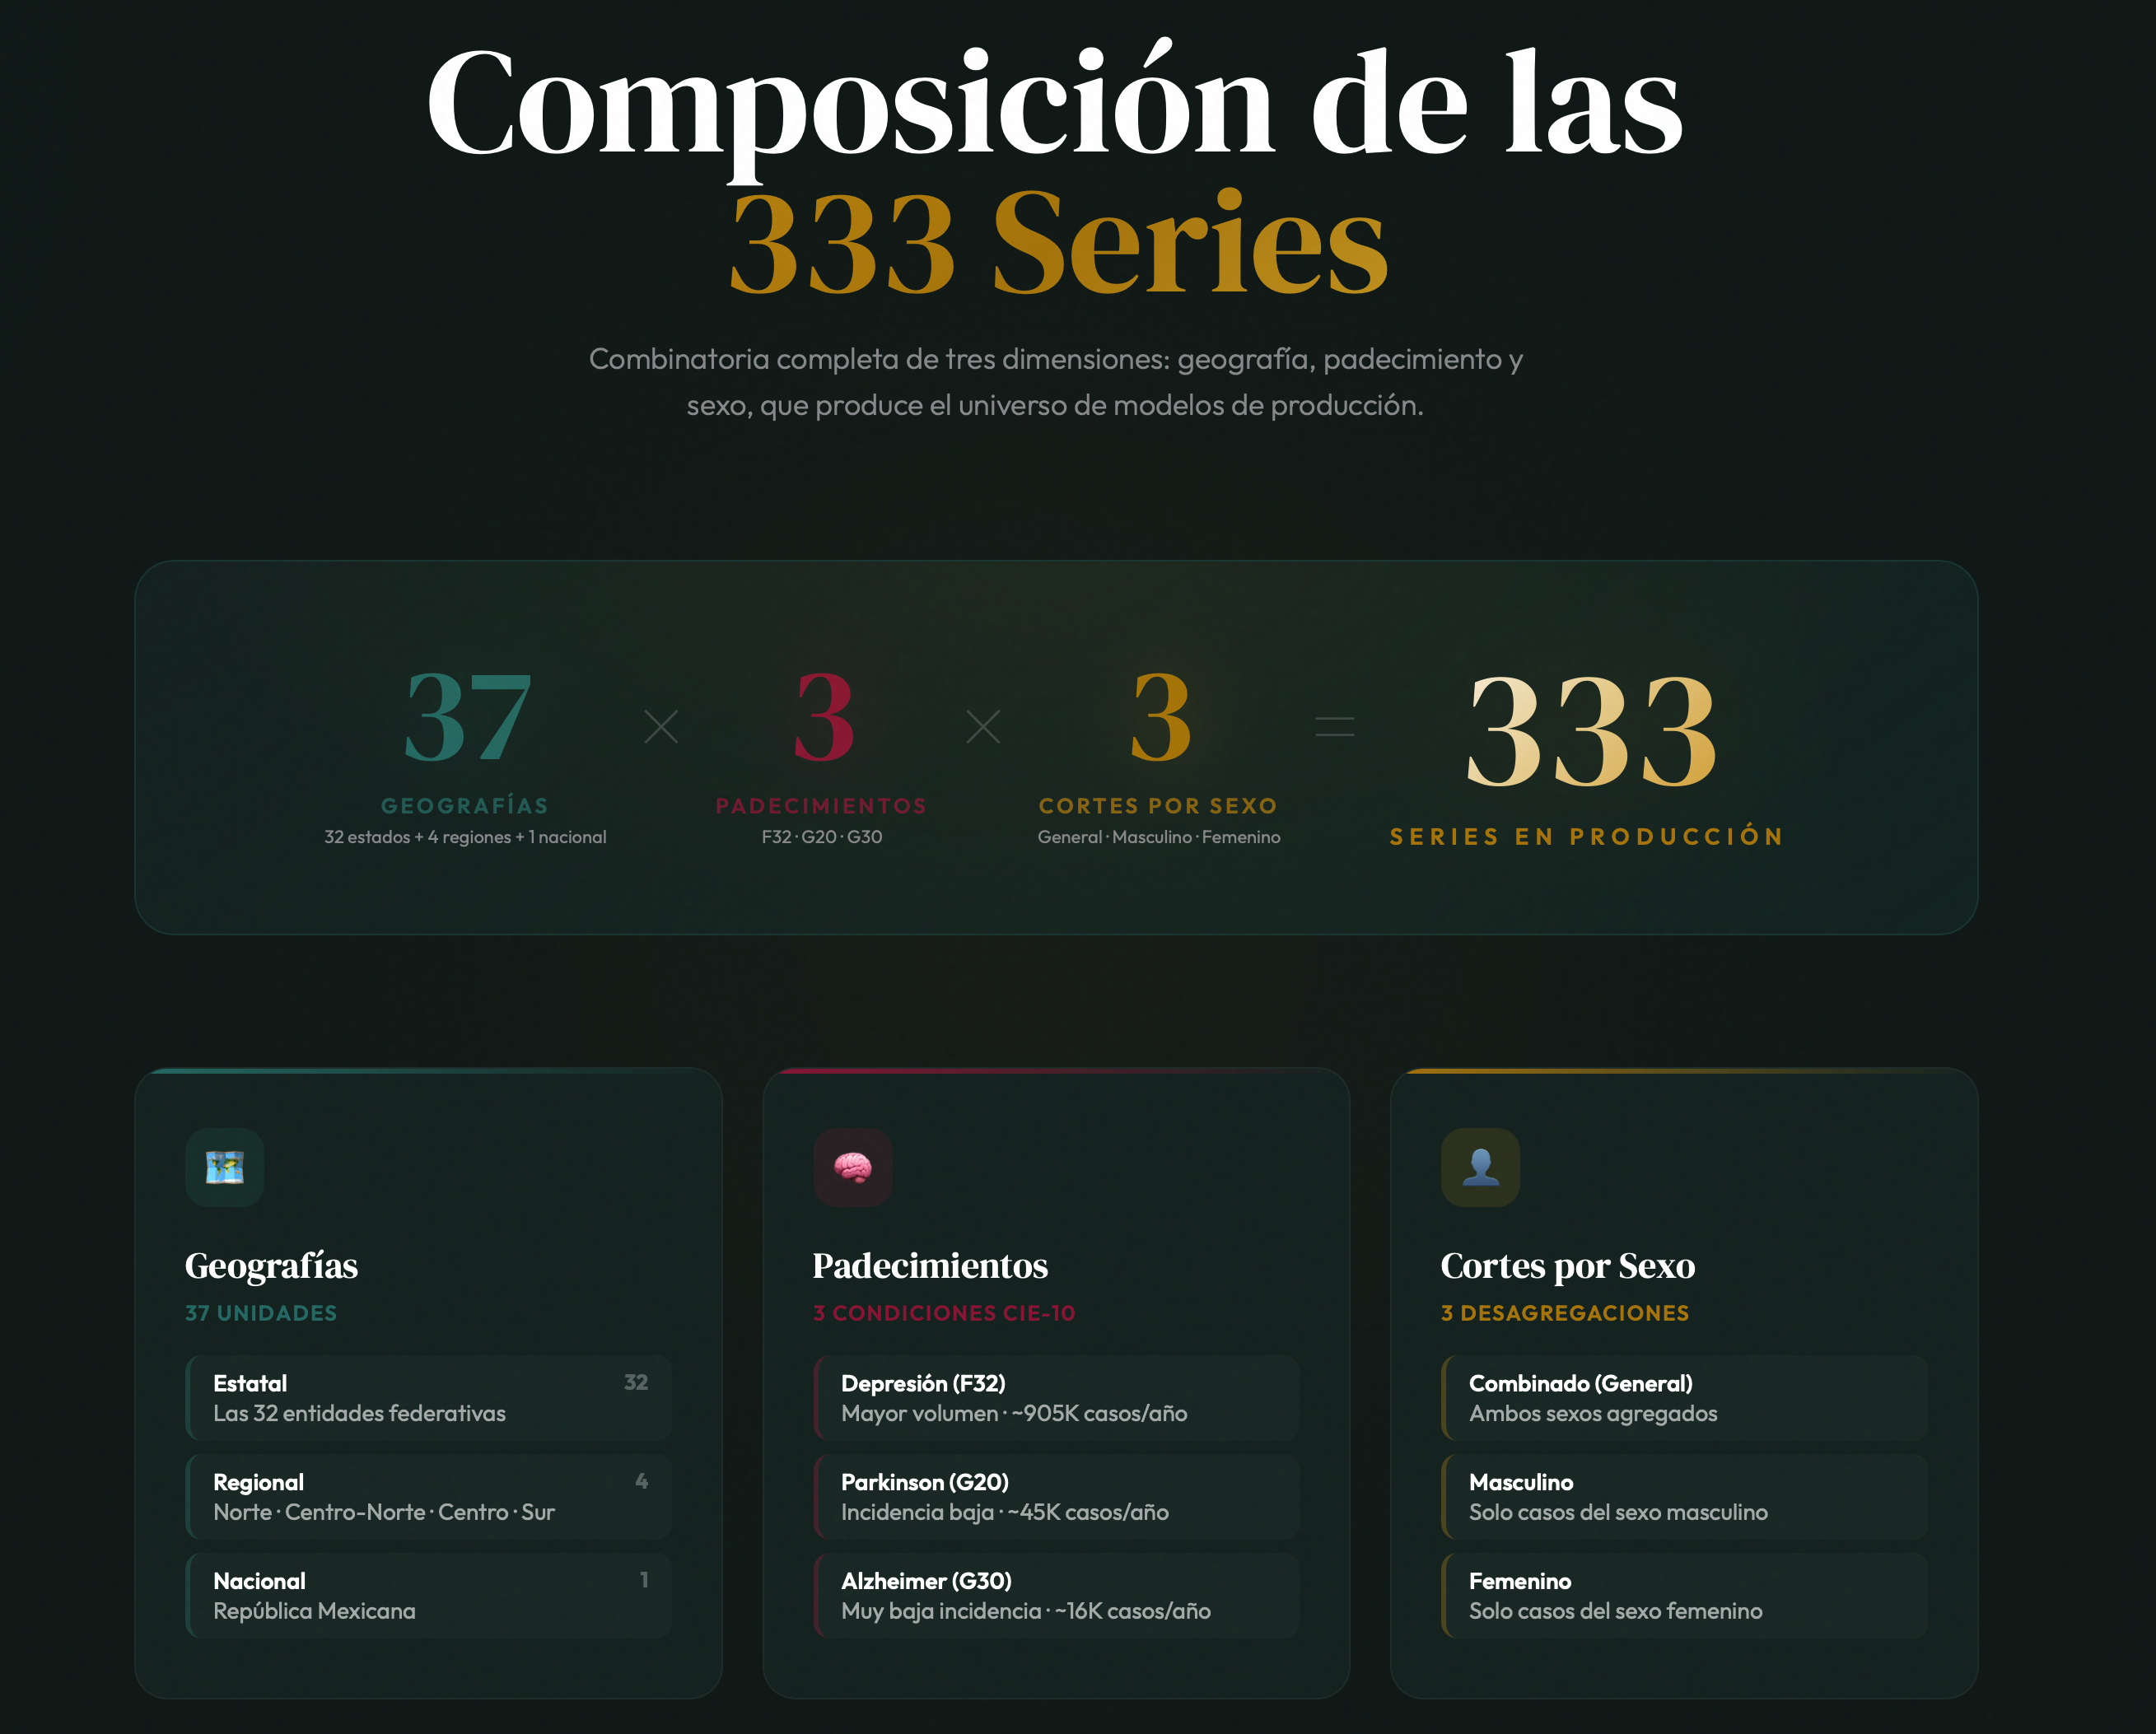
\includegraphics[width=0.95\textwidth]{fig_tendencia_3_5_cortes.png}
\caption[Composición visual de las 333 series.]{Visualización de las tres dimensiones combinatorias (37 geografías $\times$ 3 padecimientos $\times$ 3 cortes por tipo) que producen las 333 series de producción de EpiForecast-MX.}
\label{fig:composicion_visual}
\end{figure}

\begin{table}[H]
\centering
\caption{Desglose de las 333 series de producción por nivel geográfico}
\label{tab:composicion}
\small
\begin{tabularx}{\textwidth}{X c c c r}
\toprule
\textbf{Nivel geográfico} & \textbf{Geografías} & \textbf{$\times$ Pad.} & \textbf{$\times$ Casuística} & \textbf{= Series} \\
\midrule
Estatal (32 entidades)  & 32 & 3 & 3 & 288 \\
Regional (4 regiones de salud mental) & 4 & 3 & 3 & 36 \\
Nacional (República Mexicana) & 1 & 3 & 3 & 9 \\
\midrule
\textbf{Total} & \textbf{37} & & & \textbf{333} \\
\bottomrule
\end{tabularx}
\end{table}

\subsection{Regiones de salud mental}

Las cuatro regiones de salud mental, construidas por el equipo a partir de indicadores socioeconómicos y demográficos del INEGI (2024), cuya distribución espacial se detalla en la \figref{fig:mapa_regiones}, agrupan a los 32 estados según su perfil epidemiológico y urbanización:

\begin{figure}[H]
\centering
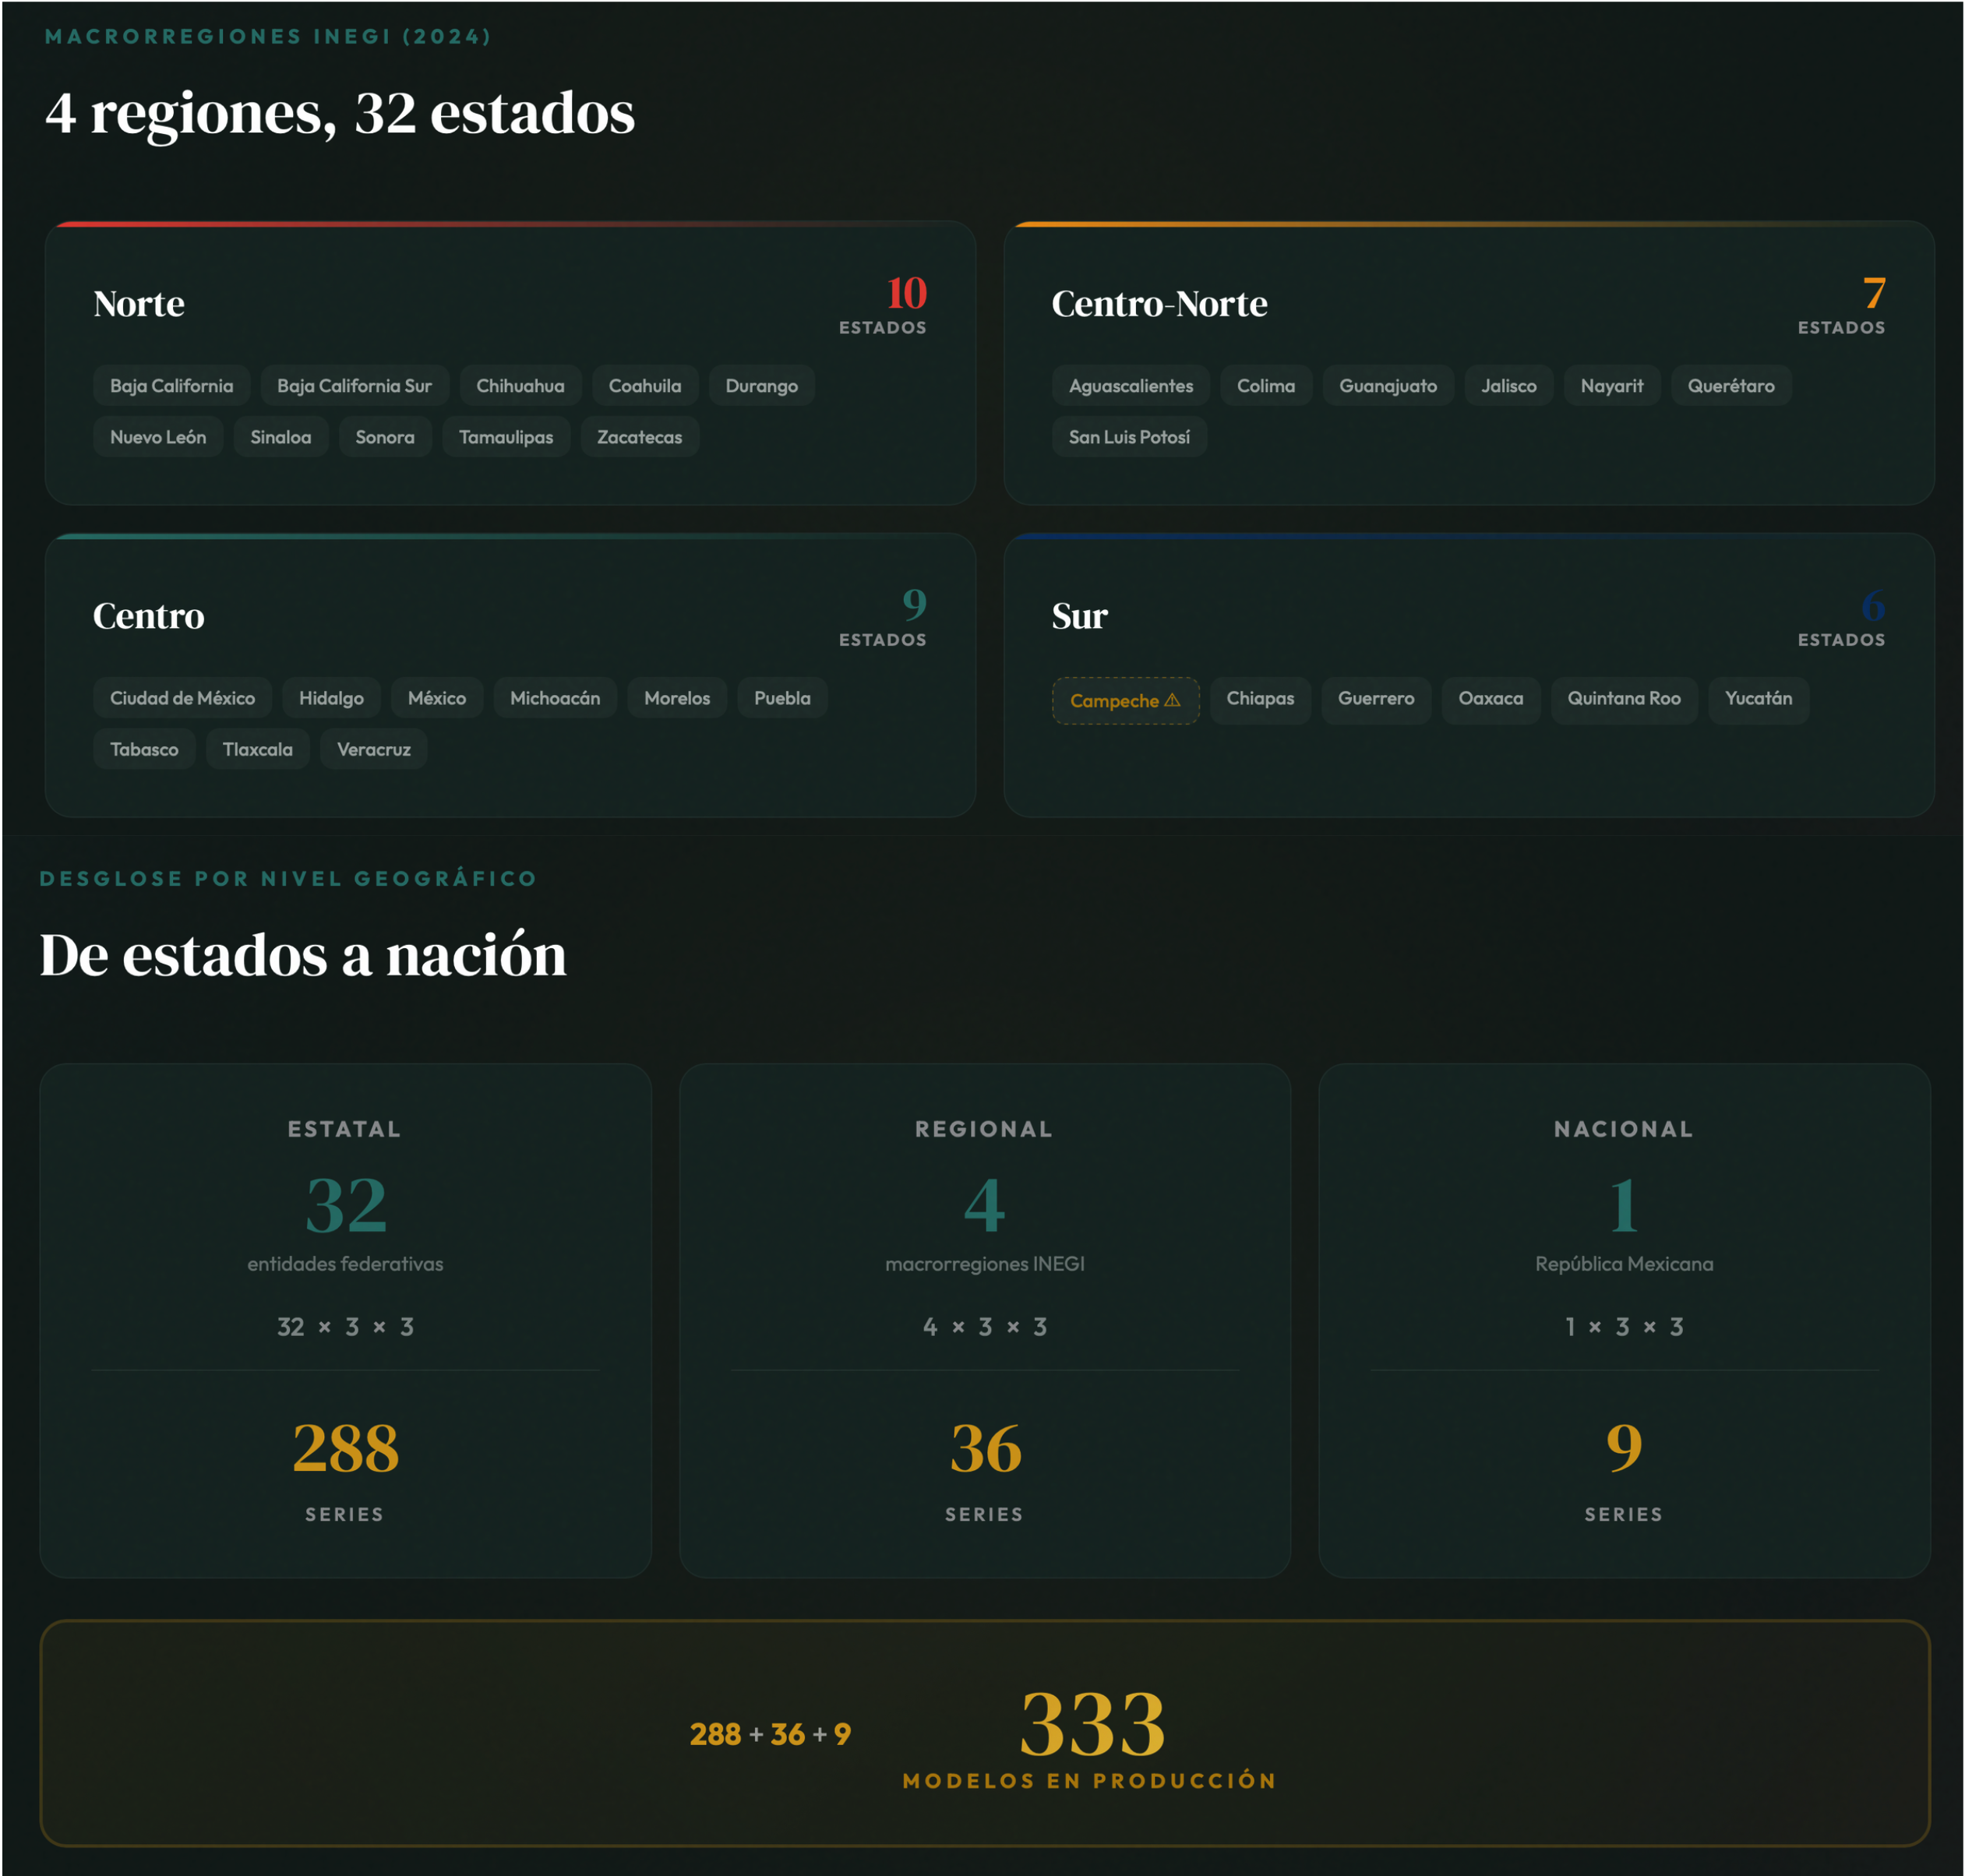
\includegraphics[width=0.85\textwidth]{fig_mapa_regiones_inegi.png}
\caption[Mapa de regiones de salud mental.]{Regiones de salud mental utilizadas para la agregación de series de pronóstico (Metropolitana alta, Urbana media, Rural/dispersa y Sur-Sureste vulnerable).}
\label{fig:mapa_regiones}
\end{figure}

\begin{table}[H]
\centering
\caption{Regiones de salud mental con entidades federativas}
\label{tab:regiones}
\scriptsize
\setlength{\tabcolsep}{3pt}
\begin{tabularx}{\textwidth}{>{\bfseries}l c X}
\toprule
\textbf{Región} & \textbf{Estados} & \textbf{Entidades} \\
\midrule
Metropolitana alta & 4 & Ciudad de México, Jalisco, México, Nuevo León \\
Urbana media & 15 & Aguascalientes, Baja California, Baja California Sur, Chihuahua, Coahuila, Colima, Durango, Guanajuato, Morelos, Querétaro, San Luis Potosí, Sinaloa, Sonora, Tamaulipas, Zacatecas \\
Rural / dispersa & 7 & Guerrero, Hidalgo, Michoacán, Nayarit, Puebla, Tlaxcala, Veracruz \\
Sur-Sureste vulnerable & 6 & Campeche, Chiapas, Oaxaca, Quintana Roo, Tabasco, Yucatán \\
\bottomrule
\end{tabularx}
\end{table}

\begin{insightbox}[¿Por qué 333 y no 288?]
Los 45 modelos adicionales (36 regionales + 9 nacionales) cumplen dos funciones críticas:
\begin{enumerate}[noitemsep]
    \item \textbf{Fallback para series con datos insuficientes}: 8 de las 333 series utilizan el modelo regional en lugar del estatal, porque la incidencia estatal es demasiado baja ($<$5 casos en 52 semanas) para entrenar un modelo confiable. Esto afecta a 7 series de Alzheimer y 1 de Parkinson (Campeche).
    \item \textbf{Contexto agregado}: las series regionales y nacionales proveen al {\imss} de una visión macro para la planificación de recursos a nivel central.
\end{enumerate}
\end{insightbox}

\newpage
% =============================================================================
% 4. INFRAESTRUCTURA MLOPS
% =============================================================================
\section{Infraestructura MLOps}\label{sec:mlops}

\subsection{Estructura del proyecto}

EpiForecast-MX sigue la plantilla \textit{Cookiecutter Data Science v2}, adaptada para un pipeline de series de tiempo multimodelo. Para garantizar la escalabilidad, se ha implementado una organización jerárquica modular que segmenta claramente el código fuente de la configuración y los datos. En la \figref{fig:estructura} se detalla la composición de los módulos principales del repositorio.

Como complemento a esta visión estructural, la \figref{fig:cookiecutter_ui} muestra la implementación real bajo el estándar \textit{Cookiecutter}, resaltando la segregación de responsabilidades entre la infraestructura \textit{cloud} (\texttt{aws/}) y la lógica de ejecución (\texttt{scripts/}). Los archivos en la raíz (\texttt{Makefile}, \texttt{pyproject.toml}) garantizan la reproducibilidad total del entorno.

\begin{figure}[H]
\centering
\begin{tikzpicture}[
    scale=0.9, transform shape, % <--- Ajusta este valor (ej. 0.8 o 1.0) para cambiar el tamaño global fácilmente
    % Estilos de nodos compactos
    dir/.style={
        draw=teal, fill=lightgreen, rounded corners=2pt, thick,
        minimum width=3.5cm, minimum height=0.5cm,
        font=\small\ttfamily, align=left,
        text width=3.1cm, anchor=west
    },
    file/.style={
        draw=coolgray, fill=cream, rounded corners=2pt, thick,
        minimum width=3.5cm, minimum height=0.5cm,
        font=\footnotesize\ttfamily, align=left,
        text width=3.1cm, anchor=west
    },
    % Estilo de las flechas
    arrow/.style={
        -{Stealth[length=4pt]}, thick, color=coolgray
    }
]

    % 1. Directorio Raíz
    \node[dir] (root) at (0, 0) {\textbf{EpiForecast-MX/}};

    % 2. Nivel 1 (Directorios principales - Espaciado reducido a 0.8)
    \node[dir] (config)  at (0.8, -0.8) {config/};
    \node[dir] (nb)      at (0.8, -1.6) {notebooks/};
    \node[dir] (scripts) at (0.8, -2.4) {scripts/};
    \node[dir] (src)     at (0.8, -3.2) {src/epiforecast/};

    % 3. Nivel 2 (Submódulos dentro de src)
    \node[file] (data)   at (1.6, -4.0) {data/};
    \node[file] (eval)   at (1.6, -4.8) {evaluation/};
    \node[file] (feat)   at (1.6, -5.6) {features/};
    \node[file] (models) at (1.6, -6.4) {models/};
    \node[file] (utils)  at (1.6, -7.2) {utils/};
    \node[file] (viz)    at (1.6, -8.0) {visualization/};

    % 4. Nivel 1 (Continuación)
    \node[dir]  (tests) at (0.8, -8.8) {tests/};

    % 5. Archivos raíz (Nivel 1)
    \node[file] (make)  at (0.8, -9.6)  {Makefile};
    \node[file] (dvc)   at (0.8, -10.4) {dvc.yaml};
    \node[file] (pypr)  at (0.8, -11.2) {pyproject.toml};

    % 6. Dibujar las líneas conectores (Raíz -> Nivel 1)
    \coordinate (L1) at ([xshift=0.3cm]root.south west);

    \foreach \n in {config, nb, scripts, src, tests, make, dvc, pypr}
        \draw[arrow] (L1) |- (\n.west);

    % 7. Dibujar las líneas conectores (src -> Nivel 2)
    \coordinate (L2) at ([xshift=0.3cm]src.south west);

    \foreach \n in {data, eval, feat, models, utils, viz}
        \draw[arrow] (L2) |- (\n.west);

\end{tikzpicture}
\caption[Estructura jerárquica compacta del repositorio.]{Estructura jerárquica compacta del repositorio EpiForecast-MX.}
\label{fig:estructura}
\end{figure}

\begin{figure}[H]
\centering
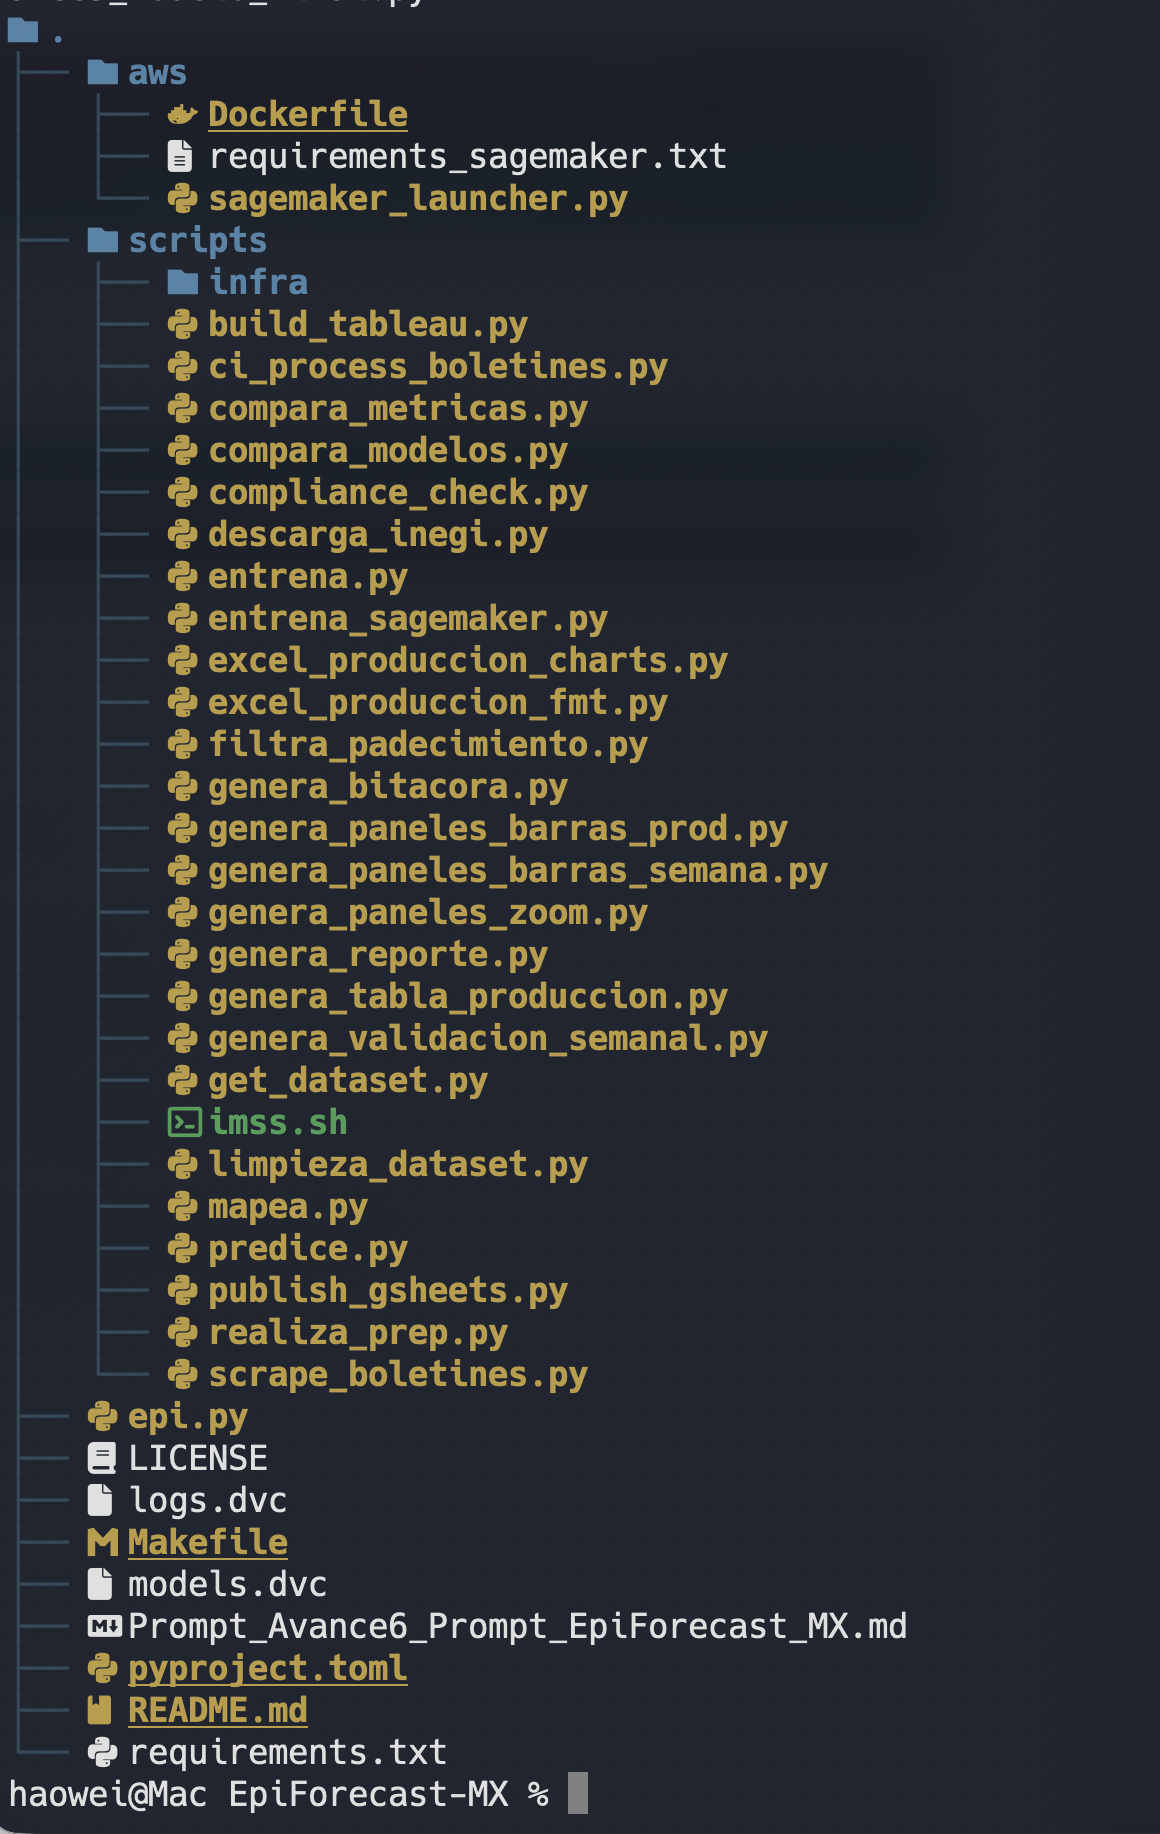
\includegraphics[width=0.6\textwidth]{04_CookieCutterRepo.png}
\caption{Vista optimizada de la arquitectura del repositorio bajo el estándar \textit{Cookiecutter Data Science v2}.}
\label{fig:cookiecutter_ui}
\end{figure}

\newpage

\subsection{Principios SOLID}

{\sloppy
El sistema de modelos implementa los cinco principios SOLID para garantizar mantenibilidad y escalabilidad:

\begin{enumerate}[noitemsep]
    \item \textbf{Single Responsibility (SRP)}: cada módulo tiene máximo 300 líneas. Los módulos extensos se segmentaron en archivos auxiliares: \texttt{prophet/\allowbreak data\_prep.py}, \texttt{ensemble/\allowbreak helpers.py}, \texttt{stacking/\allowbreak experts.py}, entre otros.
    \item \textbf{Open/Closed}: nuevos motores se integran mediante el decorador \texttt{@register\_model(\allowbreak "nombre")} sin necesidad de modificar el núcleo del sistema.
    \item \textbf{Liskov Substitution}: todos los motores heredan de la clase base \texttt{ForecastModel} e implementan la interfaz estandarizada: \texttt{fit()}, \texttt{predict()}, \texttt{cross\_validate()}, \texttt{save()} y \texttt{load()}.
    \item \textbf{Interface Segregation}: la clase base expone únicamente los métodos esenciales para el pipeline; los detalles de implementación interna permanecen encapsulados en cada motor.
    \item \textbf{Dependency Inversion}: los orquestadores de entrenamiento no dependen de clases concretas; la instanciación se centraliza en una \textit{Factory} mediante \texttt{create\_model(\allowbreak name, \allowbreak **kwargs)}.
\end{enumerate}
}

\begin{figure}[H]
    \centering
    \resizebox{0.9\textwidth}{!}{%
    \begin{tikzpicture}[
        node distance=2.2cm,
        box/.style={
            rectangle,
            rounded corners=6pt,
            draw=white,
            fill=#1,
            text=white,
            font=\sffamily\small,
            text width=4.2cm,
            minimum height=1.6cm,
            align=center,
            blur shadow={shadow blur steps=5}
        }
    ]

    % Título Central Institucional (Verde IMSS)
    \node[circle, draw=teal, fill=lightgreen, line width=2pt, minimum size=3.2cm, font=\sffamily\bfseries, align=center] (core) at (0,0) {\large ARQUITECTURA\\\Large SOLID\\ \footnotesize EpiForecast-MX};

    % SRP - Single Responsibility (Verde IMSS)
    \node[box=teal, above=of core] (srp) {
        \textbf{S: Responsabilidad Única}\\
        \scriptsize Módulos SRP $\leq$ 300 líneas.\\ \texttt{data\_prep.py} | \texttt{helpers.py}
    };

    % OCP - Open/Closed (Dorado IMSS)
    \node[box=gold, right=3.5cm of core] (ocp) {
        \textbf{O: Abierto / Cerrado}\\
        \scriptsize Extensibilidad vía decorador\\ \texttt{@register\_model}
    };

    % LSP - Liskov Substitution (Teal Oscuro)
    \node[box=darkteal, below right=1.5cm and 1cm of core] (lsp) {
        \textbf{L: Sustitución Liskov}\\
        \scriptsize Interfaz estándar unificada\\ \texttt{ForecastModel(fit, predict)}
    };

    % ISP - Interface Segregation (Guinda Institucional)
    \node[box=burgundy, below left=1.5cm and 1cm of core] (isp) {
        \textbf{I: Segregación Interfaz}\\
        \scriptsize Abstracción del Pipeline.\\ Métodos desacoplados por motor.
    };

    % DIP - Dependency Inversion (Dorado Institucional)
    \node[box=gold, left=3.5cm of core] (dip) {
        \textbf{D: Inversión Dependencias}\\
        \scriptsize Fábrica de Modelos\\ \texttt{ModelFactory.create\_model()}
    };

    % Conexiones elegantes en gris IMSS
    \foreach \n in {srp, ocp, lsp, isp, dip}
        \draw[thick, coolgray, -{Stealth[scale=1.2]}] (core) -- (\n);

    \end{tikzpicture}
    }
\caption[Principios SOLID del proyecto.]{Principios SOLID del proyecto.}
    \label{fig:solid_diagram}

\end{figure}

\newpage

\subsection{Clean Code}

\begin{itemize}[noitemsep]
    \item \textbf{Linter}: Ruff con longitud máxima de 99 caracteres, orientado a Python 3.12.
    \item \textbf{Tipado estático}: Verificación rigurosa con \texttt{mypy} en modo estricto (\textit{strict mode}) en todo el repositorio.
    \item \textbf{Formato automático}: Estilo consistente mediante \textit{Ruff format} integrado en el ciclo de vida de desarrollo.
    \item \textbf{Documentación}: Uso de \textit{docstrings} en todas las interfaces públicas; comentarios estratégicos en lógica compleja.
\end{itemize}

\begin{figure}[H]
\centering
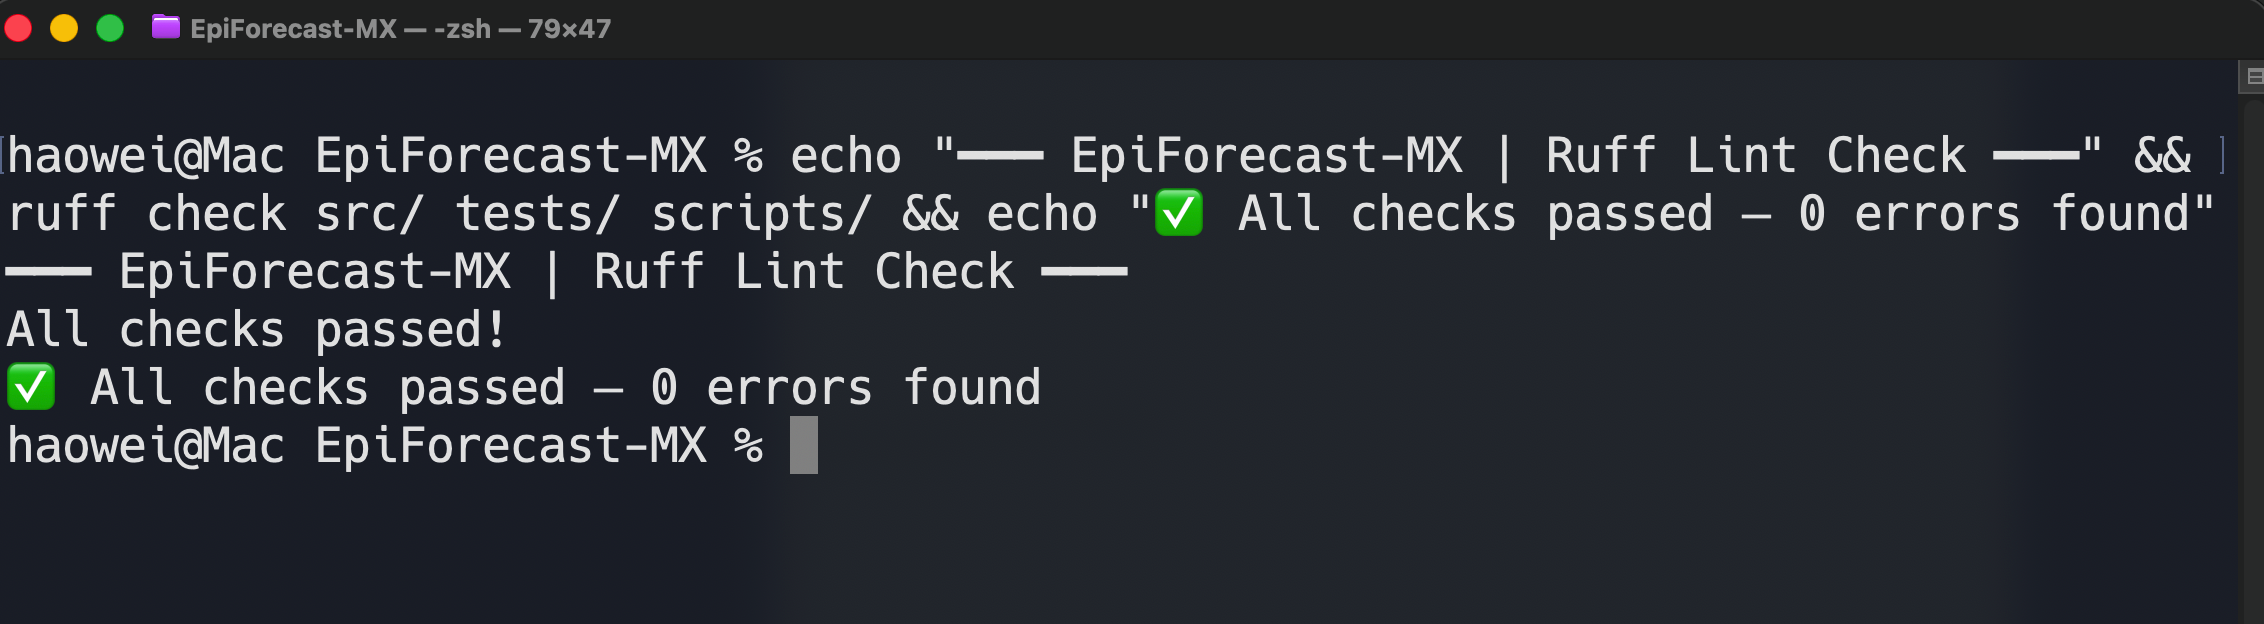
\includegraphics[width=0.85\textwidth]{fig_ruff_lint_clean.png}
\caption[Reporte de linter Ruff.]{Ejecución de \texttt{ruff check} sobre el codebase completo sin errores detectados.}
\label{fig:ruff_clean}
\end{figure}

\begin{figure}[H]
\centering
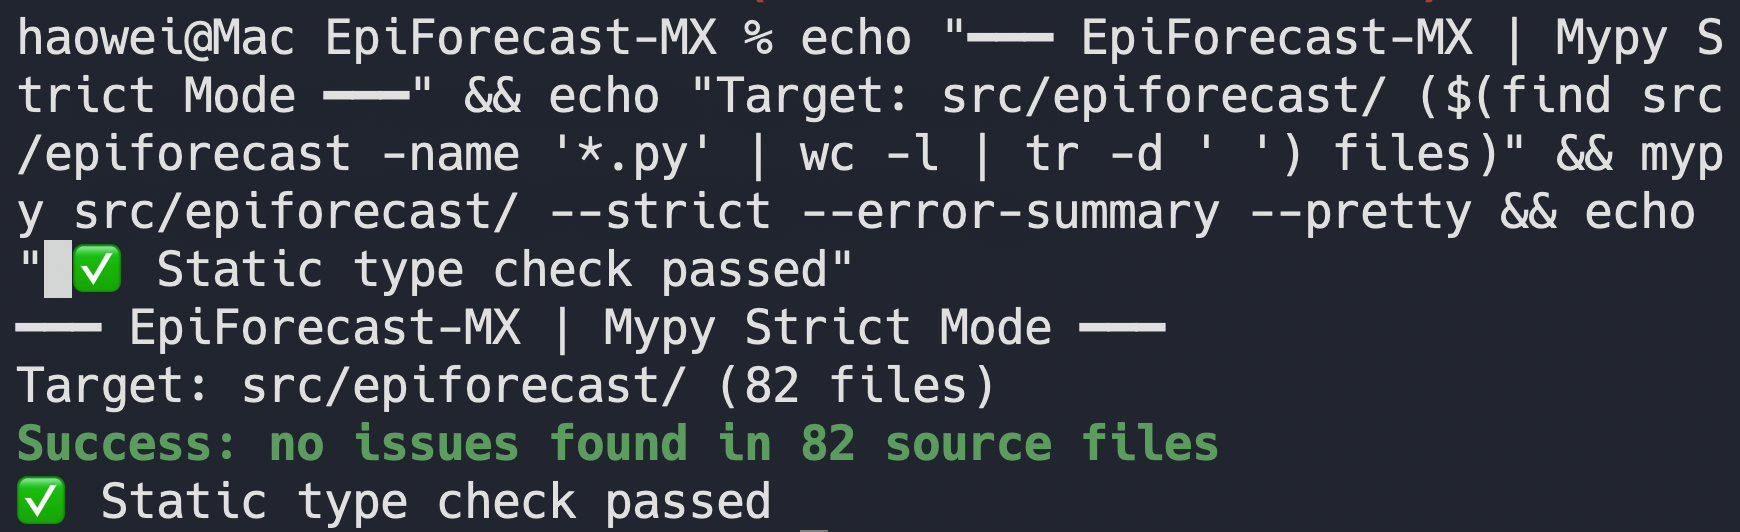
\includegraphics[width=0.85\textwidth]{fig_mypy_clean.png}
\caption[Reporte de tipado Mypy.]{Ejecución de \texttt{mypy} en modo estricto, validando la integridad de tipos estáticos.}
\label{fig:mypy_clean}
\end{figure}

\subsection{CI/CD con GitHub Actions}

El pipeline de integración continua, cuyos resultados se visualizan en la \figref{fig:github_ci}, ejecuta tres verificaciones en cada push y pull request:

\begin{enumerate}[noitemsep]
    \item \textbf{Lint}: \texttt{ruff check} verifica estilo y convenciones.
    \item \textbf{Typecheck}: \texttt{mypy} valida tipos estáticos.
    \item \textbf{Tests}: \texttt{pytest} ejecuta 855 pruebas (849 unitarias, 3 de integración y 3 lentas).
\end{enumerate}

\begin{figure}[H]
\centering
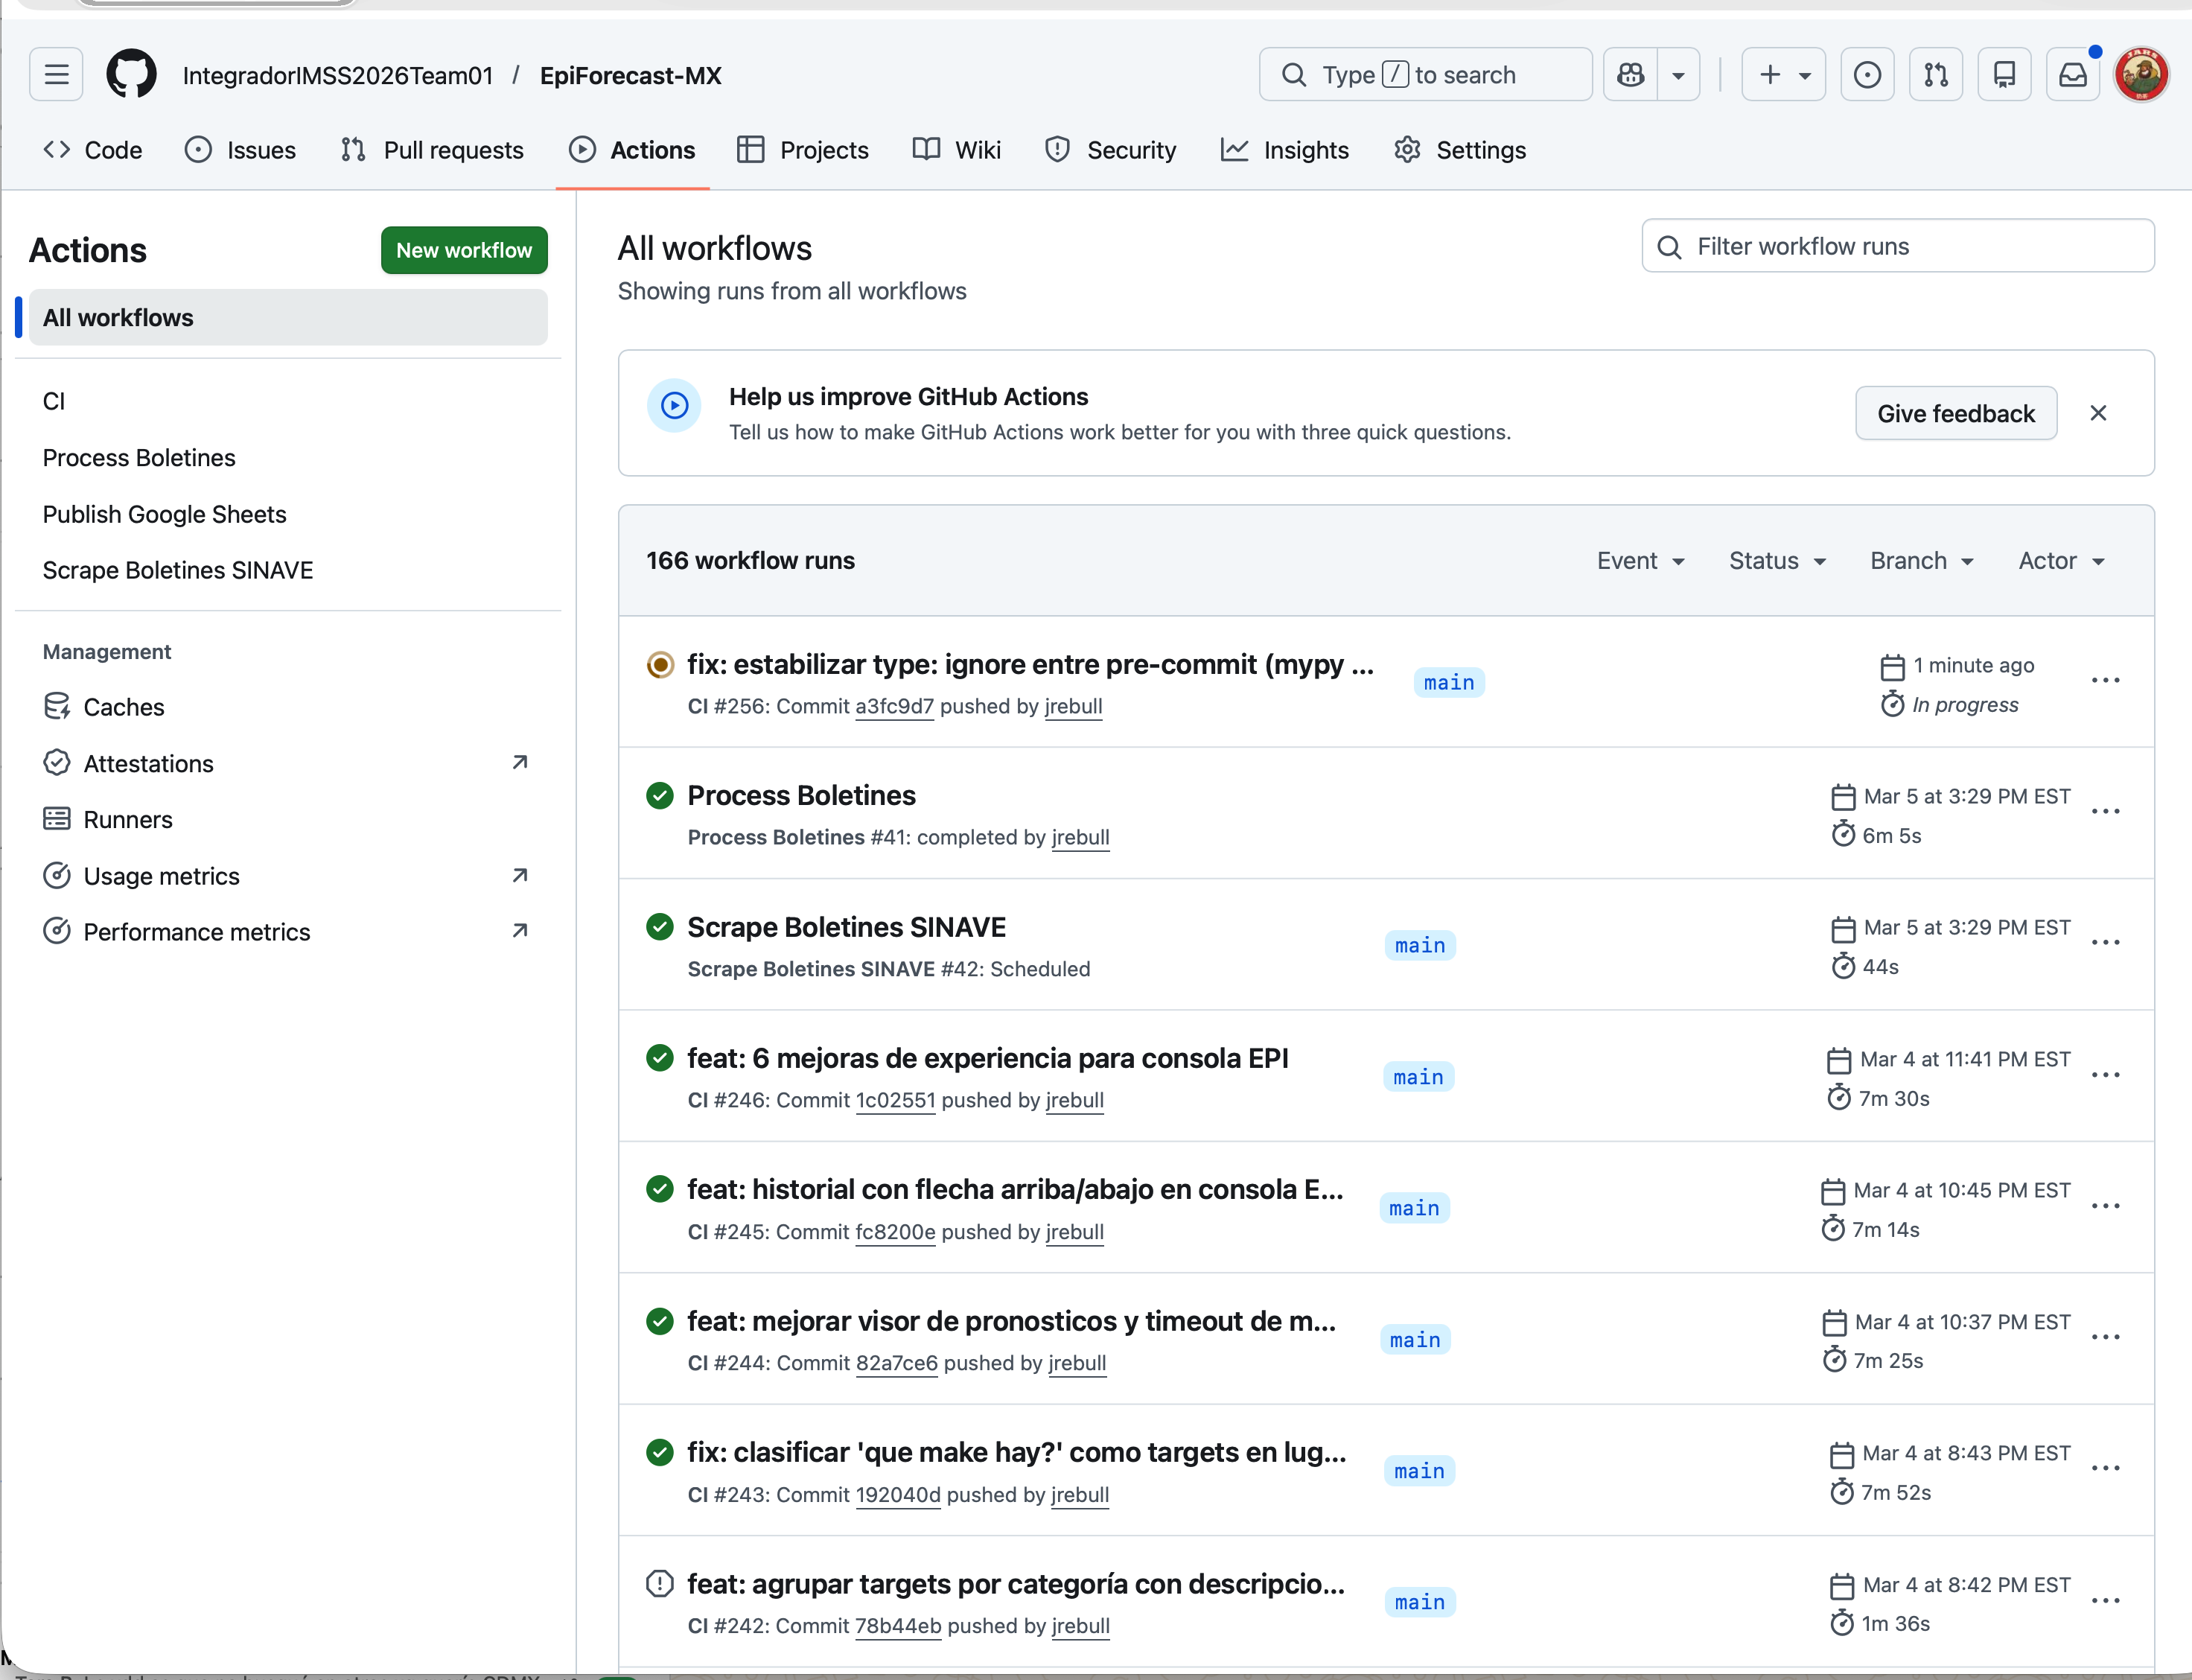
\includegraphics[width=0.95\textwidth]{fig_github_actions_ci.png}
\caption[Pipeline de CI/CD en GitHub.]{Pipeline de CI/CD en GitHub Actions mostrando los tres checks (lint, typecheck, tests) ejecutados exitosamente.}
\label{fig:github_ci}
\end{figure}

Como parte del flujo de versionado, cada hito del proyecto se marca con \textit{tags} semánticos en Git que documentan la evolución del sistema desde la primera versión funcional hasta la configuración final de producción (\figref{fig:github_tags}).

\begin{figure}[H]
\centering
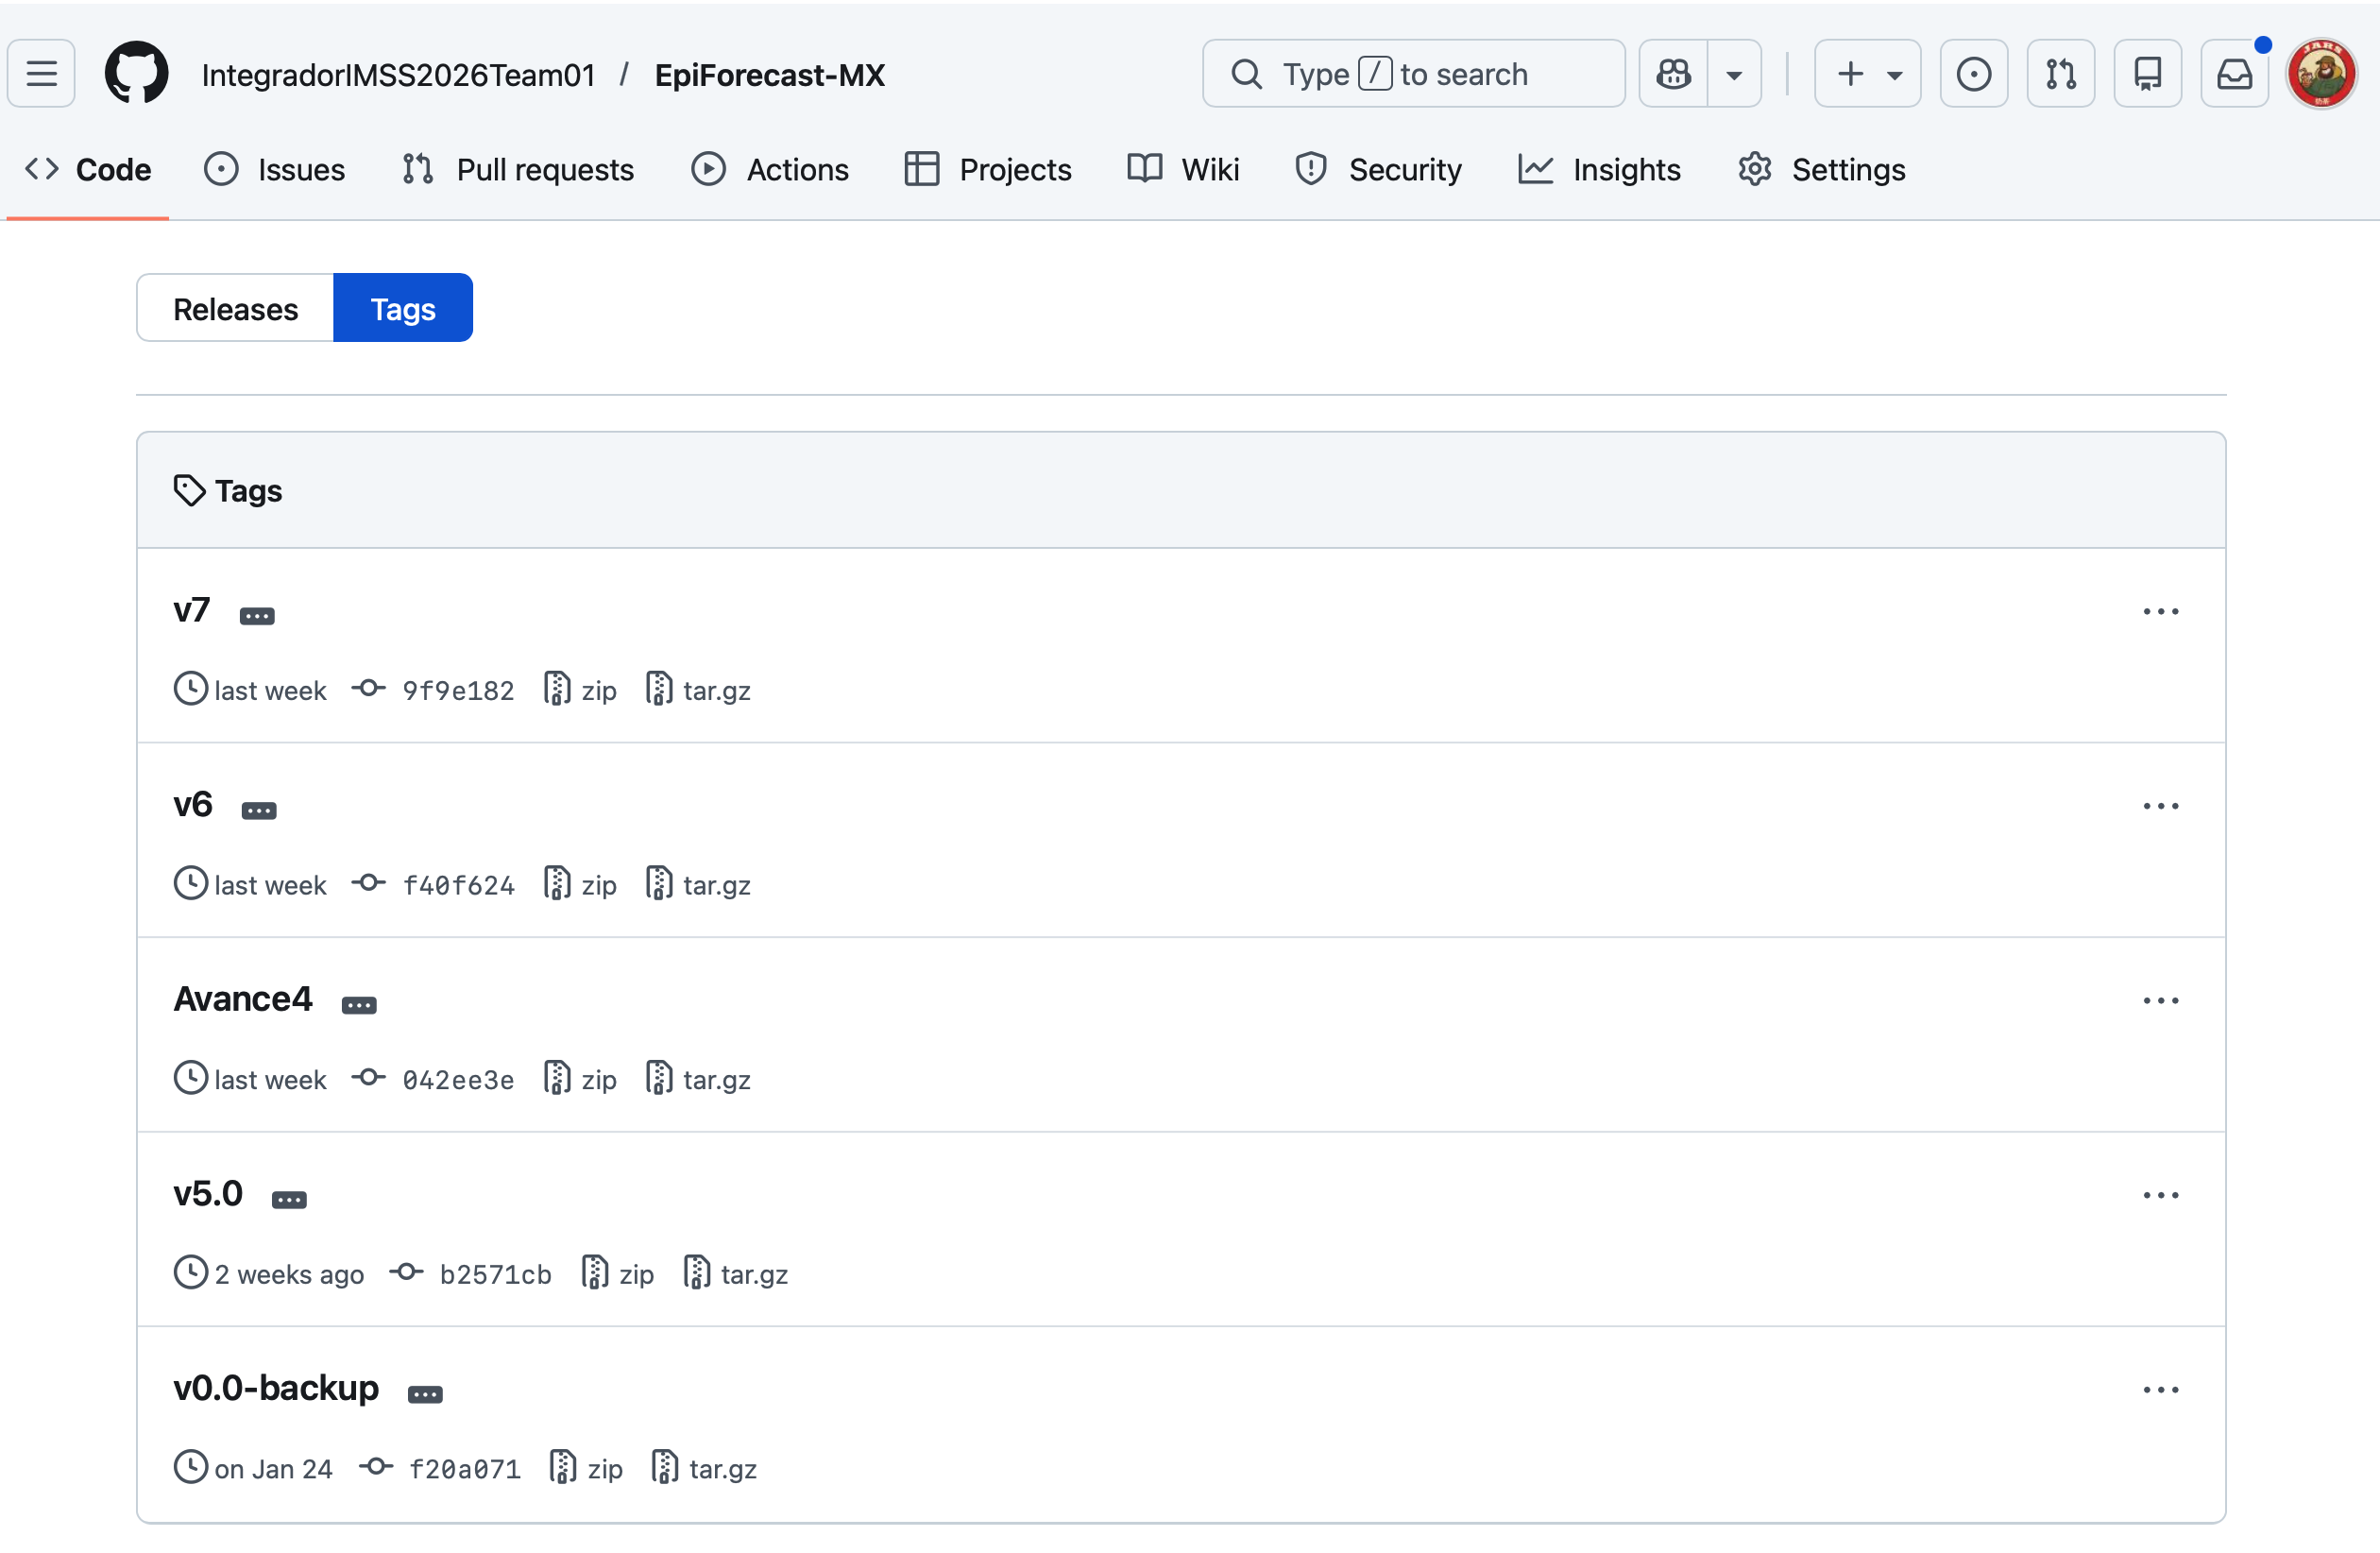
\includegraphics[width=0.95\textwidth]{fig_github_tags.png}
\caption[Historial de tags en GitHub.]{Historial de tags semánticos del repositorio, documentando los hitos principales del ciclo de desarrollo de EpiForecast-MX.}
\label{fig:github_tags}
\end{figure}

\subsection{EPI Console: más de 50 comandos Make}

El \texttt{Makefile} centraliza todas las operaciones del pipeline MLOps, desde la descarga de datos hasta el despliegue en SageMaker. Como se observa en la \figref{fig:epiconsole}, esto permite que cualquier miembro del equipo reproduzca el pipeline completo con un solo comando.

\begin{figure}[H]
\centering
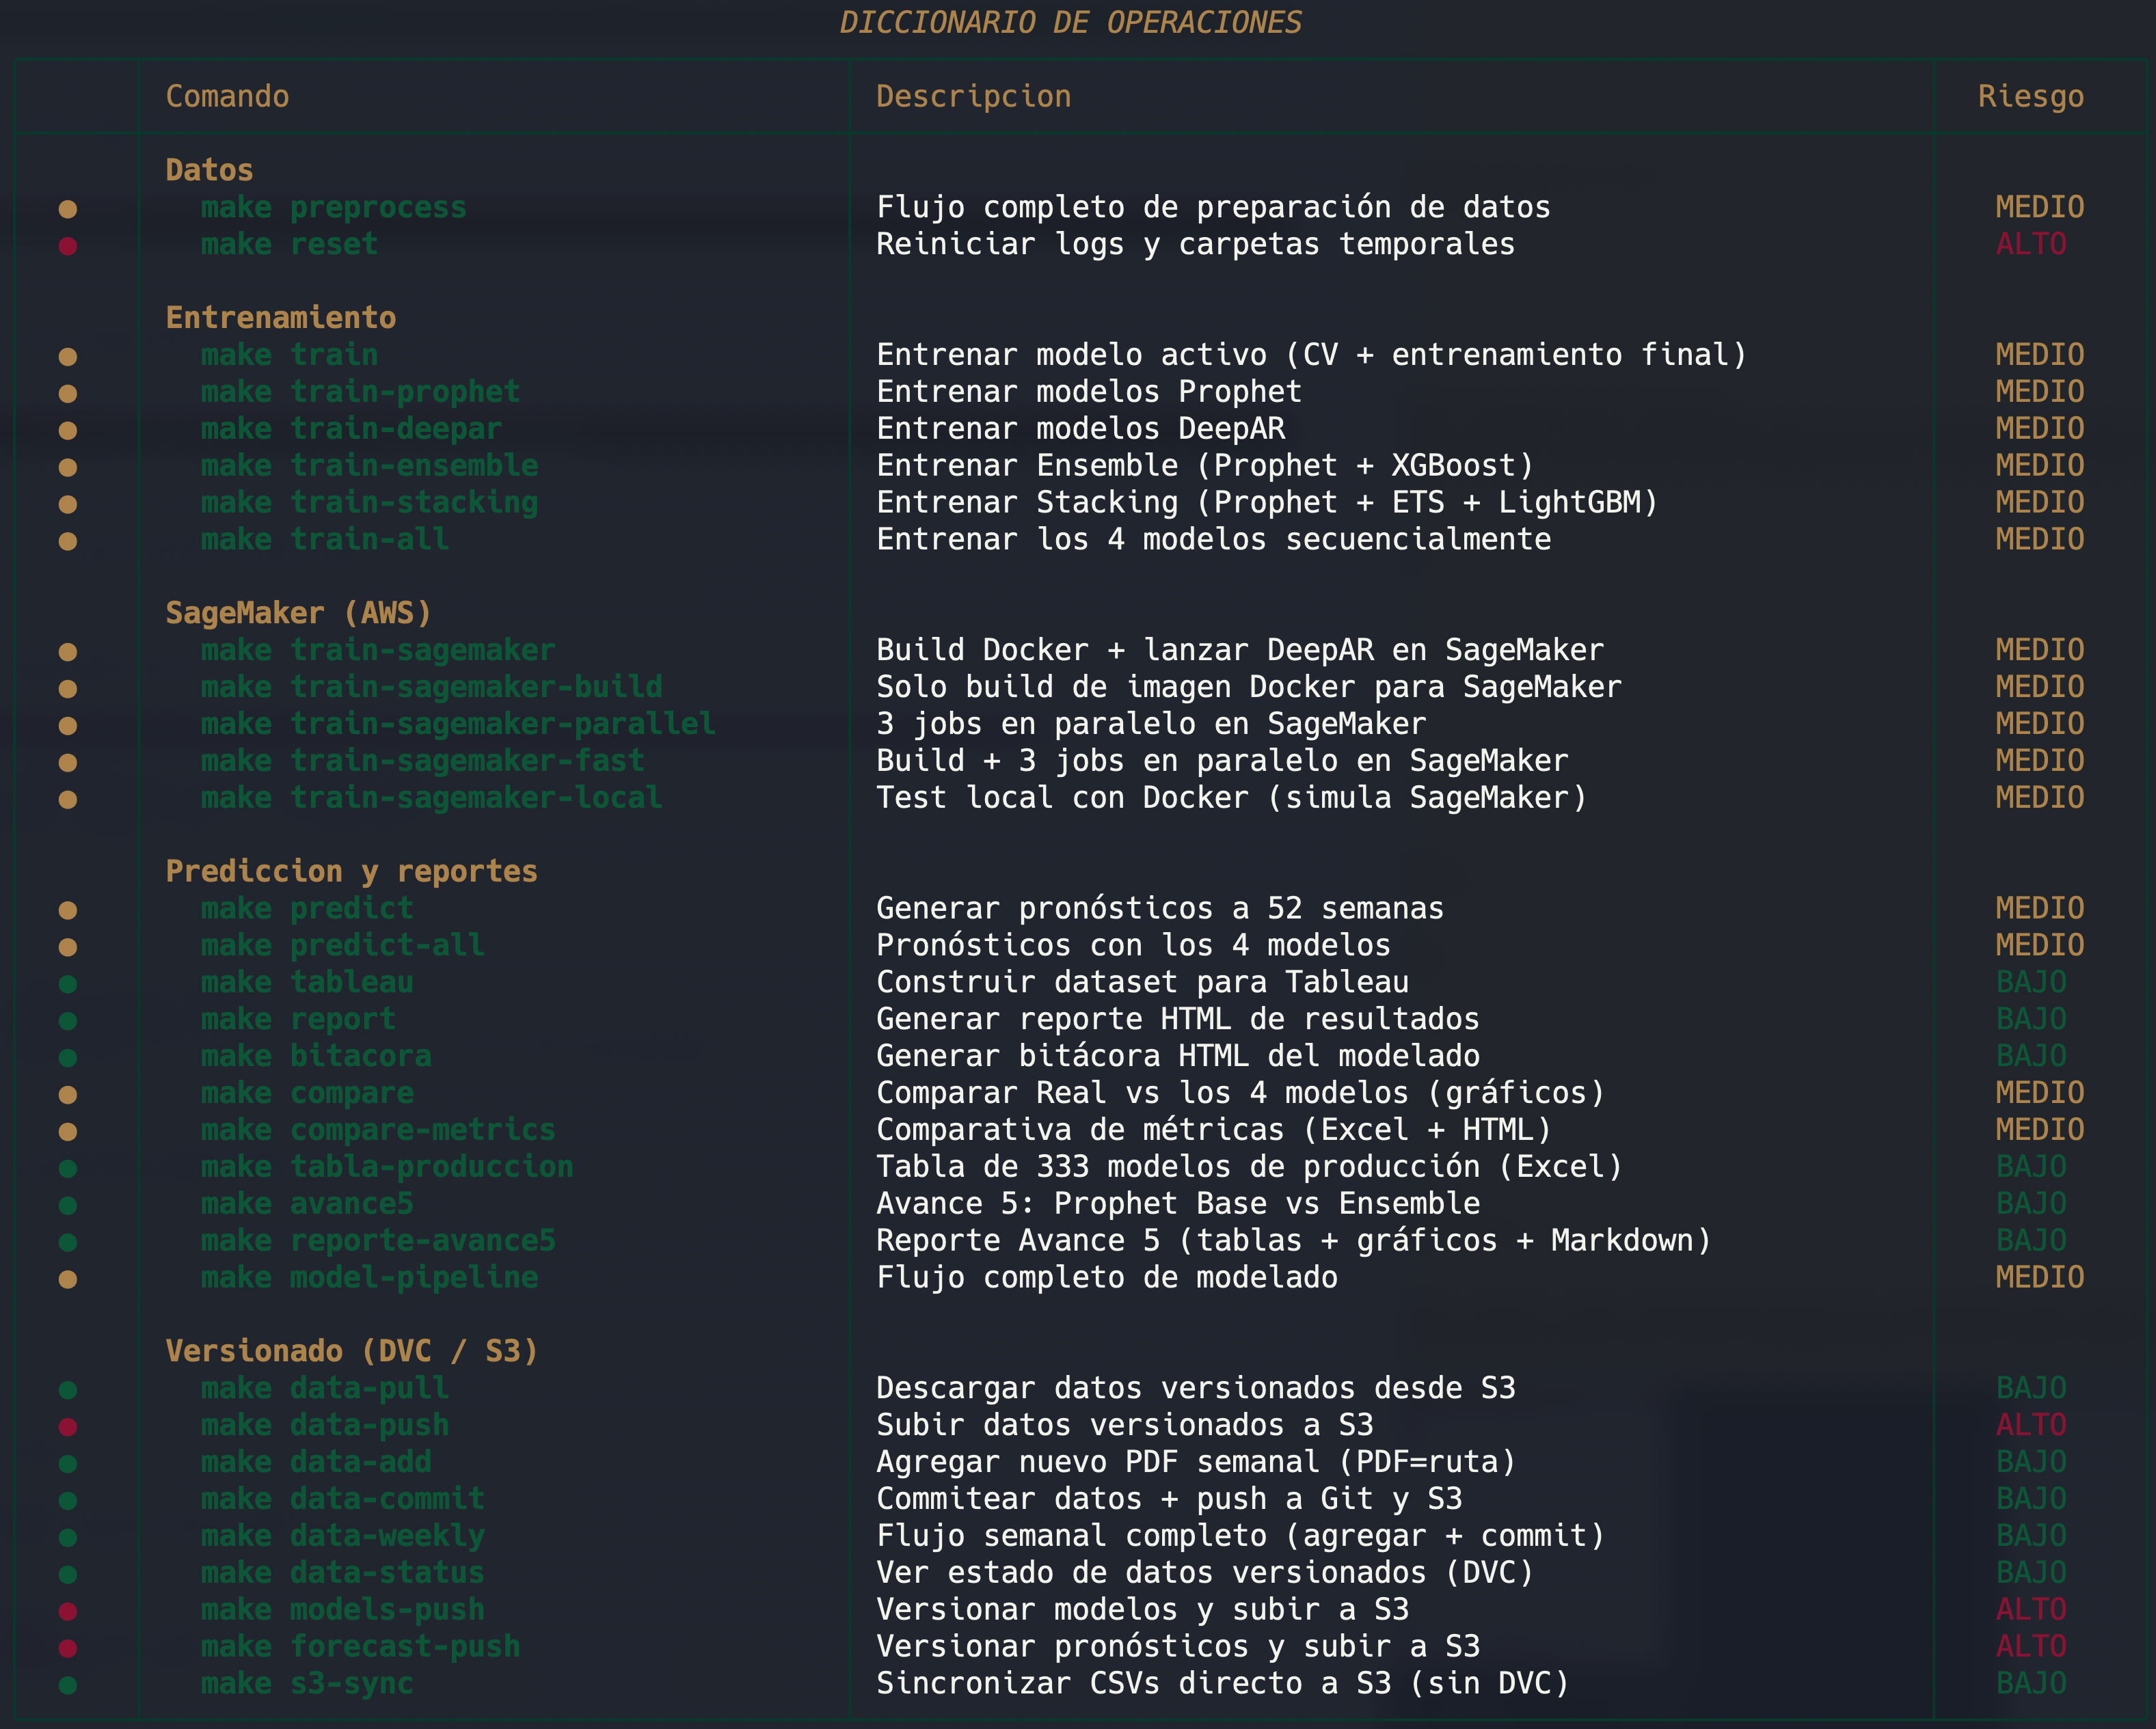
\includegraphics[width=0.95\textwidth]{fig_epiconsole_help.png}
\caption[Interfaz de EPI Console.]{Salida del comando \texttt{make help} mostrando la EPI Console con los más de 50 comandos disponibles organizados por categoría.}
\label{fig:epiconsole}
\end{figure}

\begin{table}[H]
\centering
\caption{Comandos principales de la EPI Console}
\label{tab:epiconsole}
\scriptsize
\setlength{\tabcolsep}{3pt}
\begin{tabularx}{\textwidth}{>{\ttfamily}l X}
\toprule
\textbf{Comando} & \textbf{Descripción} \\
\midrule
make preprocess & Pipeline completo de limpieza y mapeo INEGI \\
make train-all & Entrena los 4 motores secuencialmente (Prophet, DeepAR, Ensemble, Stacking) \\
make predict-all & Genera pronósticos de los 4 modelos \\
make compare & Gráficos comparativos Real vs 4 modelos \\
make compare-metrics & Excel + HTML con badges de overfitting y leakage \\
make tableau & Dataset Tableau con selección automática de modelo productivo \\
make quality & Lint + typecheck + tests \\
make train-sagemaker & Build Docker + entrenamiento DeepAR en GPU (SageMaker) \\
make data-pull & Descarga datos desde S3 vía DVC \\
make report & Reporte HTML de resultados \\
\bottomrule
\end{tabularx}
\end{table}

La referencia completa de comandos se encuentra en el Apéndice~\ref{sec:comandos}.

\subsection{DVC y versionado de datos}

Los datos y modelos se versionan con DVC (Data Version Control) respaldado en AWS S3 (\texttt{s3://epiforecast-mx-data}), lo que permite una trazabilidad completa del pipeline (\figref{fig:dvc_dag}) y una organización granular de los artefactos (\figref{fig:s3_bucket}).

\begin{figure}[H]
\centering
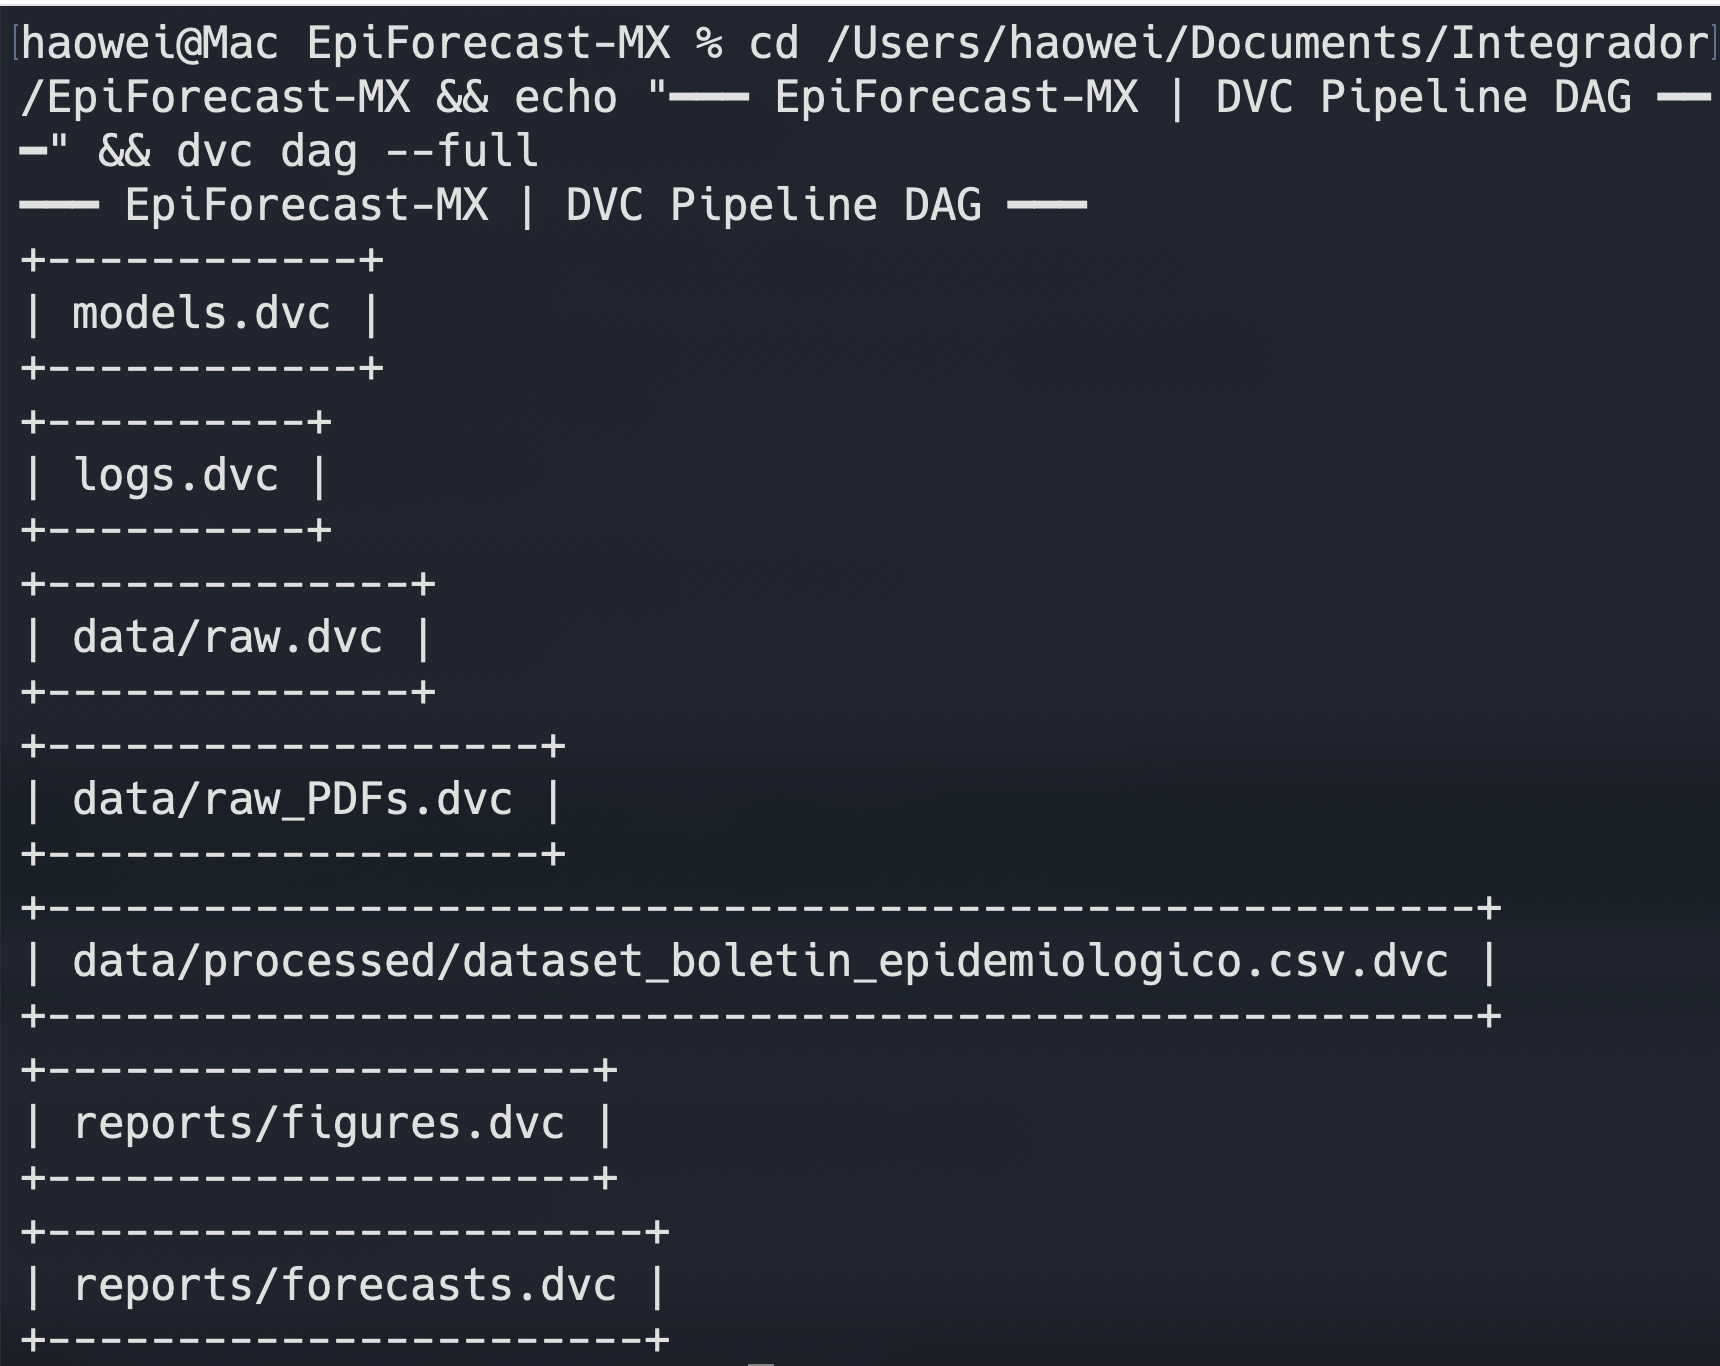
\includegraphics[width=0.80\textwidth]{fig_dvc_dag.png}
\caption[Grafo de dependencias DVC.]{Grafo acíclico dirigido (DAG) generado por \texttt{dvc dag}, mostrando las dependencias entre etapas del pipeline.}
\label{fig:dvc_dag}
\end{figure}

\begin{figure}[H]
\centering
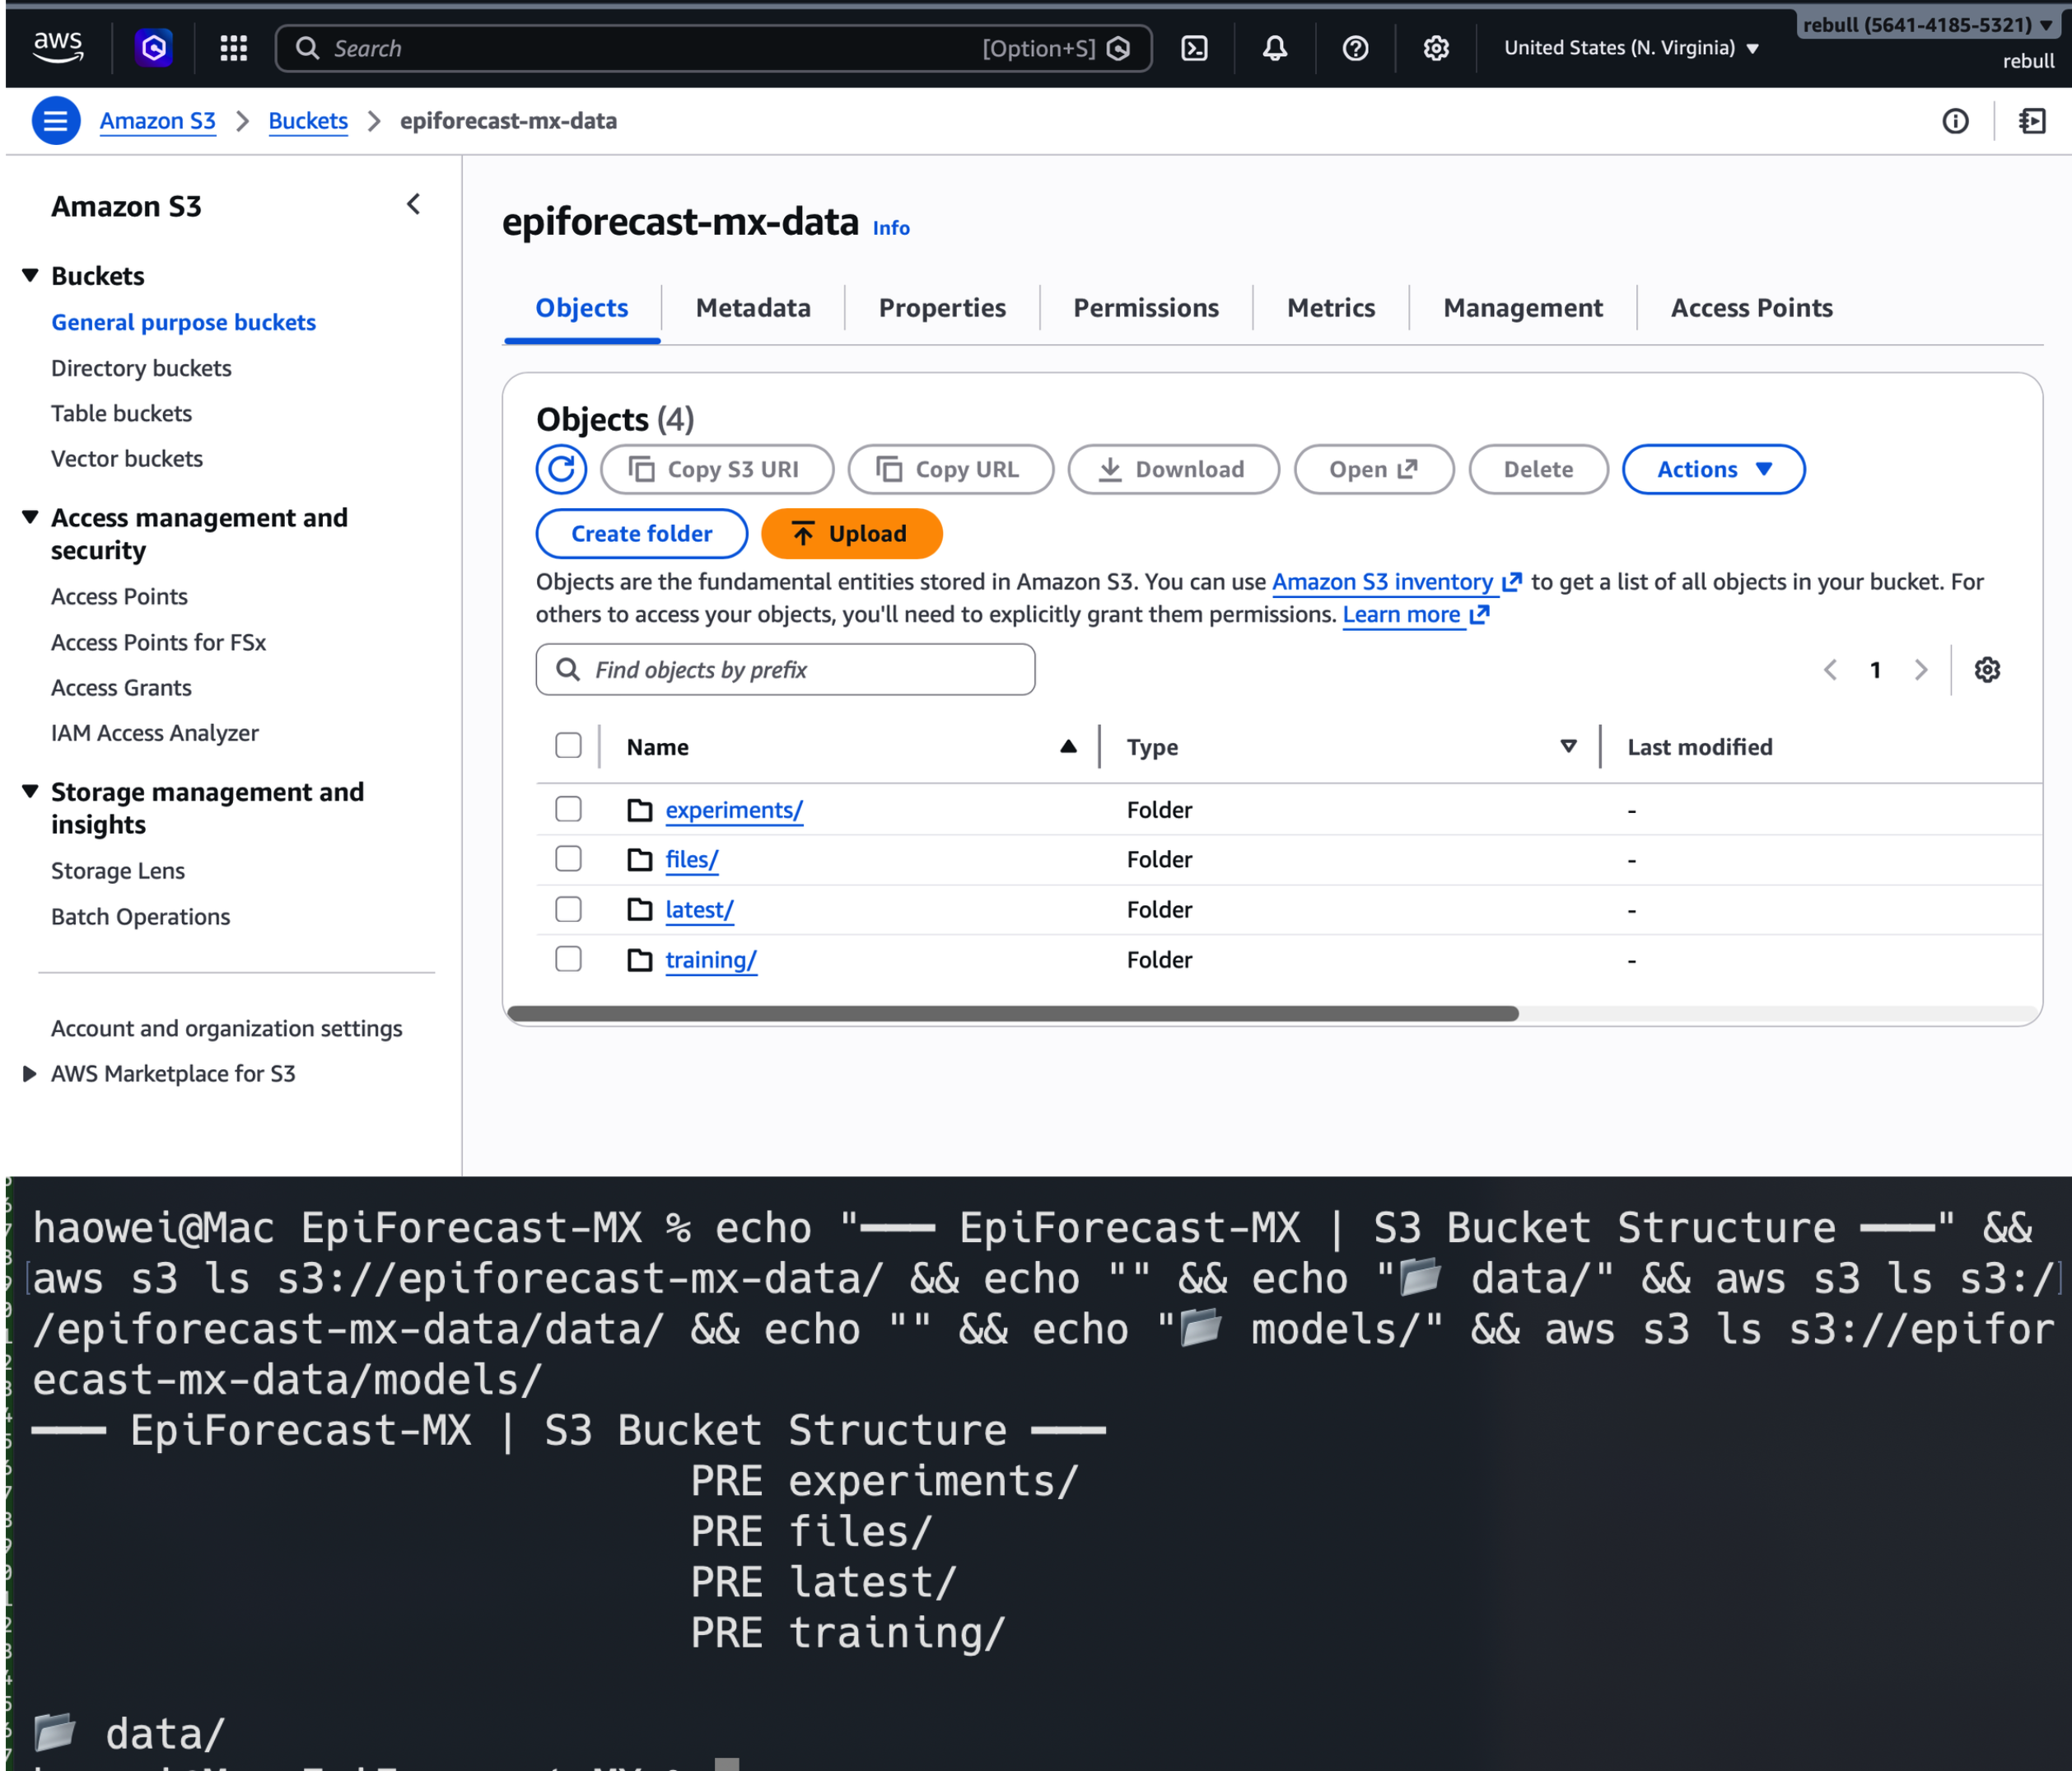
\includegraphics[width=0.90\textwidth]{fig_s3_bucket_structure.png}
\caption[Estructura del bucket AWS S3.]{Estructura del bucket S3 \texttt{epiforecast-mx-data} mostrando las carpetas de datos y modelos versionados.}
\label{fig:s3_bucket}
\end{figure}

\subsection{Testing: 855 pruebas automatizadas}

El suite de pruebas cubre 46 archivos con 855 funciones de test:

\begin{table}[H]
\centering
\caption{Distribución de pruebas por categoría}
\label{tab:tests}
\small
\begin{tabularx}{\textwidth}{l r X}
\toprule
  \textbf{Categoría} & \textbf{Tests} & \textbf{Descripción} \\
  \midrule
  Unitarias (rápidas) & 849 & Funciones puras, lógica de negocio, helpers \\
  Integración & 3 & Pipeline end-to-end, compatibilidad entre módulos \\
  Lentas (\texttt{@slow}) & 3 & Entrenamiento real de modelos, validación cruzada \\
  \midrule\textbf{Total} & \textbf{855} & Cobertura 92\% \\
\bottomrule
\end{tabularx}
\end{table}

Como se detalla en el reporte de cobertura (\figref{fig:test_coverage}), el sistema alcanza una cobertura del 92\%, garantizando la estabilidad de los módulos críticos.

\begin{figure}[H]
\centering
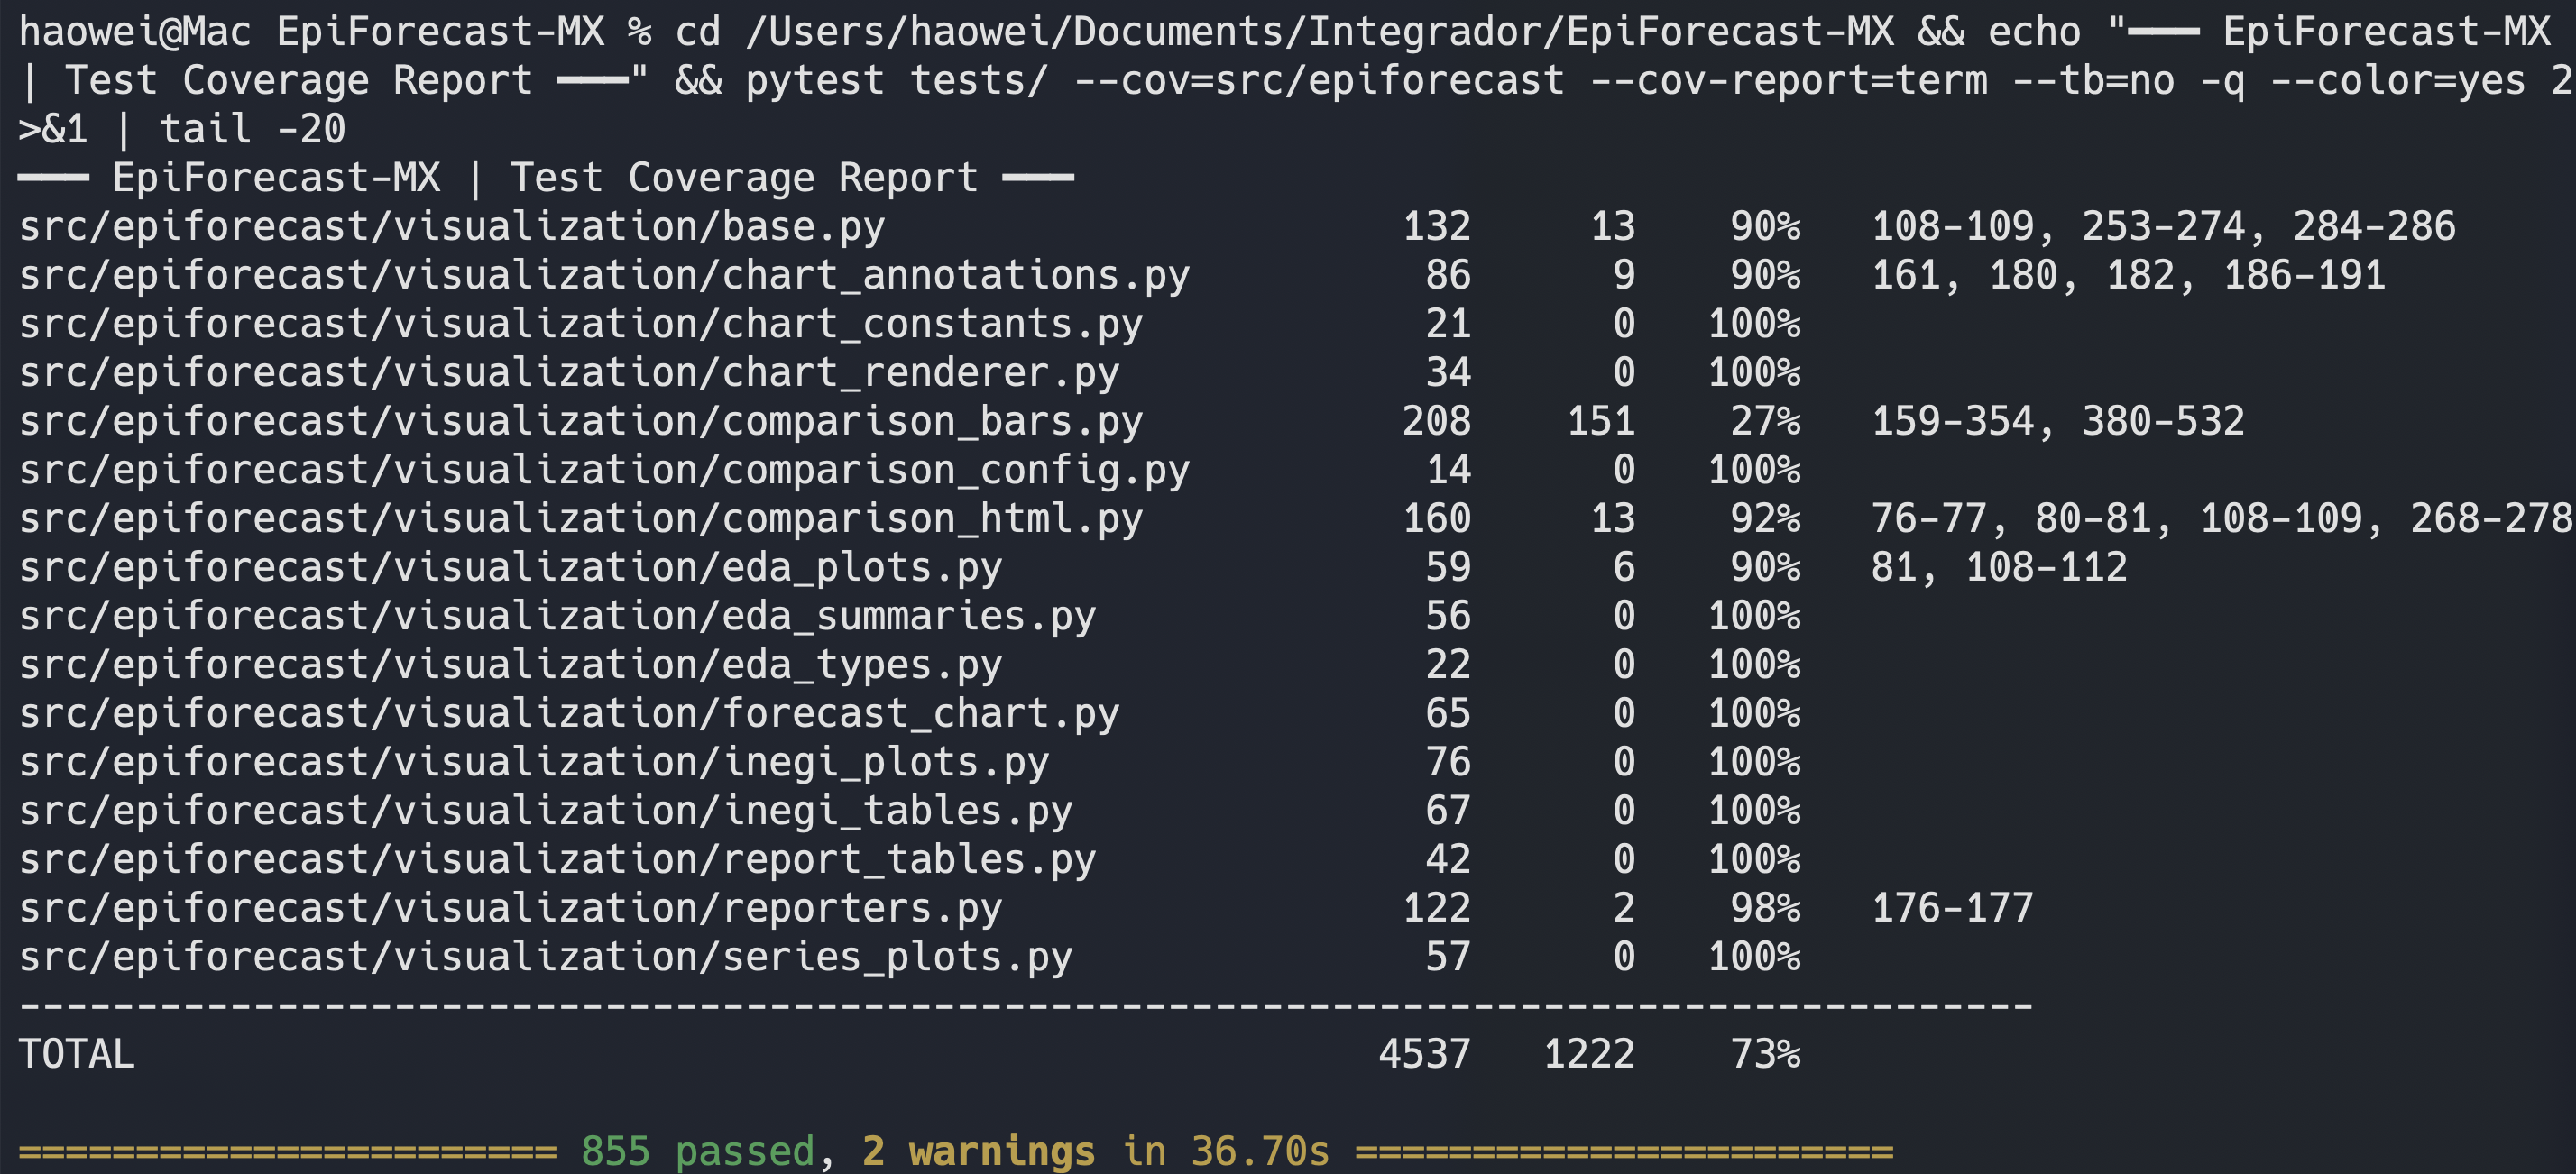
\includegraphics[width=0.95\textwidth]{fig_test_coverage.png}
\caption[Reporte de cobertura de tests.]{Reporte de cobertura generado por \texttt{pytest --cov}, mostrando una cobertura del 92\%.}
\label{fig:test_coverage}
\end{figure}

\subsection{Pre-commit hooks}

Cada commit pasa por seis verificaciones automáticas antes de ser aceptado:

\begin{enumerate}[noitemsep]
    \item Ruff check (linter)
    \item Ruff format (formato automático)
    \item mypy (tipos estáticos)
    \item Trailing whitespace
    \item Validación YAML
    \item Validación TOML
\end{enumerate}

La ejecución exitosa de estas verificaciones (\figref{fig:precommit}) previene la introducción de errores comunes y mantiene la consistencia del estilo en todo el equipo.

\begin{figure}[H]
\centering
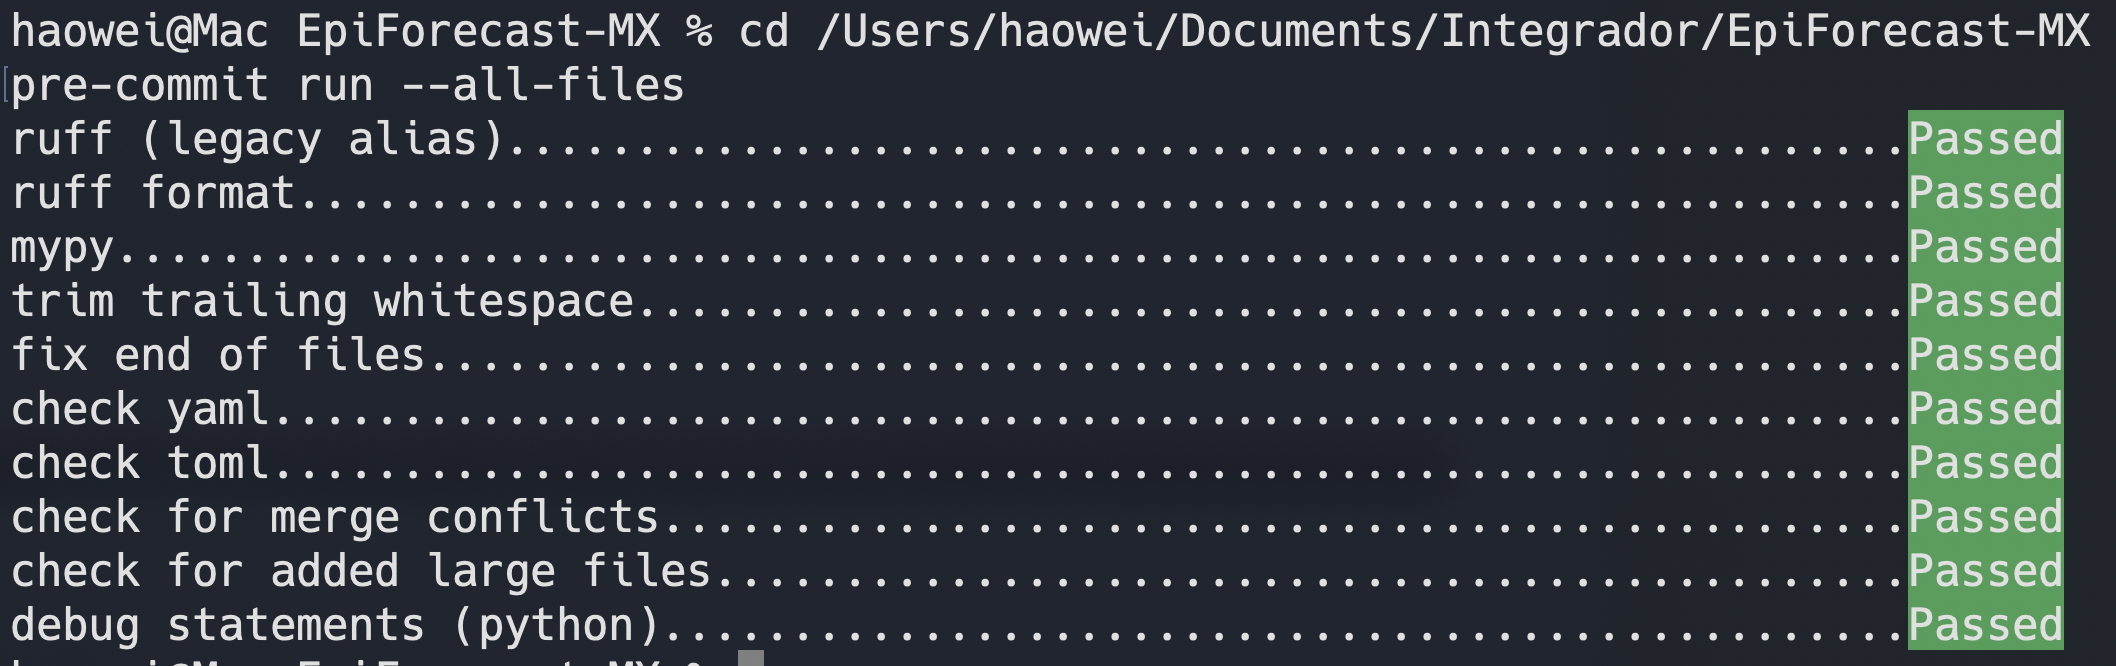
\includegraphics[width=0.85\textwidth]{fig_precommit_pass.png}
\caption[Ejecución de pre-commit hooks.]{Verificación automática de calidad (Ruff, mypy, formato) previa a la confirmación de cambios en Git.}
\label{fig:precommit}
\end{figure}

\subsection{Diagrama de arquitectura del sistema}

\begin{figure}[H]
\centering
\resizebox{\textwidth}{!}{%
\begin{tikzpicture}[
    % 1. ESTILO BASE MAESTRO: Sombras 3D sutiles, bordes suaves y fuente moderna
    base/.style={
        thick, rounded corners=6pt, align=center, font=\sffamily,
        drop shadow={opacity=0.12, shadow xshift=2pt, shadow yshift=-2pt}
    },
    % 2. BLOQUES DE COLORES (Respetando tu paleta original e igualando anchos)
    data/.style={base, draw=burgundy, fill=lightred!50,
        minimum width=2.6cm, minimum height=1.3cm, text width=2.4cm},
    block/.style={base, draw=teal, fill=lightgreen,
        minimum width=2.6cm, minimum height=1.3cm, text width=2.4cm},
    model/.style={base, draw=gold, fill=lightyellow,
        minimum width=2.4cm, minimum height=0.9cm, text width=2.2cm},
    output/.style={base, draw=imssblue, fill=cream,
        minimum width=2.6cm, minimum height=1.3cm, text width=2.4cm},
    % 3. FLECHAS ESTILO PIPELINE DE DATOS
    arrow/.style={
        -{Stealth[round, length=8pt, width=6pt]},
        thick, color=coolgray,
        shorten >=1.5pt, shorten <=1.5pt
    },
    % 4. ETIQUETAS "PÍLDORA" FLOTANTES
    label/.style={
        font=\sffamily\scriptsize\bfseries\color{coolgray},
        fill=white, inner sep=3pt, rounded corners=4pt
    }
]
    % --- RECUADRO AGRUPADOR (Capa de Modelado) ---
    % Dibuja un límite visual elegante alrededor del cerebro del sistema
    \draw[draw=coolgray, rounded corners=8pt, dashed, thick]
        (11.8, -3.1) rectangle (15.2, 3.1);
    \node[font=\sffamily\scriptsize\bfseries\color{coolgray}, fill=white, inner sep=4pt]
        at (13.5, 3.1) {CAPA DE MODELADO};

    % --- COLUMNA 1: Fuentes de Datos (X=0) ---
    \node[data] (sinave) at (0, 1.8)  {\textbf{SINAVE}\\[1mm]\scriptsize (PDF)};
    \node[data] (inegi)  at (0, -1.8) {\textbf{INEGI}\\[1mm]\scriptsize (Población)};

    % --- COLUMNA 2: Extracción (X=4.5) ---
    \node[block] (etl) at (4.5, 0) {\textbf{ETL}\\[1mm]\scriptsize Pipeline};

    % --- COLUMNA 3: Feature Engineering (X=9) ---
    \node[block] (features) at (9, 0) {\textbf{Feature}\\[1mm]\scriptsize Engineering};

    % --- COLUMNA 4: Modelos (X=13.5, simetría perfecta en eje Y) ---
    \node[model] (prophet)  at (13.5,  2.25) {\textbf{Prophet}};
    \node[model] (deepar)   at (13.5,  0.75) {\textbf{DeepAR}};
    \node[model] (ensemble) at (13.5, -0.75) {\textbf{Ensemble}};
    \node[model] (stacking) at (13.5, -2.25) {\textbf{Stacking}};

    % --- COLUMNA 5: Selección (X=18) ---
    \node[block] (selector) at (18, 0) {\textbf{Selector}\\[1mm]\scriptsize Producción};

    % --- COLUMNA 6: Salidas (X=22.5) ---
    \node[output] (dashboard) at (22.5,  1.8) {\textbf{Dashboard}\\[1mm]\scriptsize Tableau};
    \node[output] (reportes)  at (22.5, -1.8) {\textbf{Reportes}\\[1mm]\scriptsize HTML/PDF};

    % ==========================================
    % CONEXIONES CURVAS (Flujo tipo Data Pipeline)
    % Usamos to[out=0, in=180] para crear curvas de Bézier fluidas
    % ==========================================

    % Entradas -> ETL (Fan-in orgánico)
    \draw[arrow] (sinave.east) to[out=0, in=180] node[label, pos=0.4] {scraping} (etl.west);
    \draw[arrow] (inegi.east) to[out=0, in=180] (etl.west);

    % ETL -> Features (Línea recta directa, están alineados al centro)
    \draw[arrow] (etl.east) -- node[label] {interim} (features.west);

    % Features -> Modelos (Efecto Fan-out curvo)
    \draw[arrow] (features.east) to[out=0, in=180] (prophet.west);
    \draw[arrow] (features.east) to[out=0, in=180] (deepar.west);
    \draw[arrow] (features.east) to[out=0, in=180] (ensemble.west);
    \draw[arrow] (features.east) to[out=0, in=180] (stacking.west);

    % Modelos -> Selector (Efecto Fan-in curvo)
    \draw[arrow] (prophet.east) to[out=0, in=180] (selector.west);
    \draw[arrow] (deepar.east) to[out=0, in=180] (selector.west);
    \draw[arrow] (ensemble.east) to[out=0, in=180] (selector.west);
    \draw[arrow] (stacking.east) to[out=0, in=180] (selector.west);

    % Selector -> Salidas (Divergencia orgánica final)
    \draw[arrow] (selector.east) to[out=0, in=180] (dashboard.west);
    \draw[arrow] (selector.east) to[out=0, in=180] (reportes.west);

\end{tikzpicture}
}% fin resizebox
\caption[Arquitectura general del sistema.]{Arquitectura del sistema EpiForecast-MX: del dato crudo al dashboard}
\label{fig:arquitectura}
\end{figure}

\subsection{Ingenier\'ia de features para modelos de \'arbol}\label{subsec:feature_engineering}

El componente XGBoost del Ensemble opera sobre \textbf{20 features temporales} construidas exclusivamente a partir de la serie objetivo $y$. La \tabref{tab:features_xgb} desglosa cada feature por categor\'ia.

\begin{table}[H]
\centering
\caption{Features de XGBoost en el modelo Ensemble (20 en total)}
\label{tab:features_xgb}
\small
\begin{tabularx}{\textwidth}{l l l X}
\toprule
\textbf{Categor\'ia} & \textbf{Feature} & \textbf{F\'ormula} & \textbf{Descripci\'on} \\
\midrule
\multirow{7}{*}{Lags (7)}
  & \texttt{lag\_1}  & $y_{t-1}$  & Semana anterior \\
  & \texttt{lag\_2}  & $y_{t-2}$  & Dos semanas atr\'as \\
  & \texttt{lag\_4}  & $y_{t-4}$  & Un mes atr\'as \\
  & \texttt{lag\_8}  & $y_{t-8}$  & Dos meses atr\'as \\
  & \texttt{lag\_13} & $y_{t-13}$ & Un trimestre atr\'as \\
  & \texttt{lag\_26} & $y_{t-26}$ & Un semestre atr\'as \\
  & \texttt{lag\_52} & $y_{t-52}$ & Un a\~no atr\'as \\
\midrule
\multirow{5}{*}{\shortstack[l]{Medias\\m\'oviles (5)}}
  & \texttt{roll\_4}  & $\overline{y}_{t-1}^{(4)}$  & Media de 4 semanas sobre $y_{t-1}$ \\
  & \texttt{roll\_8}  & $\overline{y}_{t-1}^{(8)}$  & Media de 8 semanas sobre $y_{t-1}$ \\
  & \texttt{roll\_12} & $\overline{y}_{t-1}^{(12)}$ & Media de 12 semanas sobre $y_{t-1}$ \\
  & \texttt{roll\_26} & $\overline{y}_{t-1}^{(26)}$ & Media de 26 semanas sobre $y_{t-1}$ \\
  & \texttt{roll\_52} & $\overline{y}_{t-1}^{(52)}$ & Media de 52 semanas sobre $y_{t-1}$ \\
\midrule
Volatilidad (1) & \texttt{roll\_std\_13} & $\sigma_{t-1}^{(13)}$ & Desv. est\'andar de 13 semanas sobre $y_{t-1}$ \\
\midrule
\multirow{4}{*}{\shortstack[l]{Calendario (4)}}
  & \texttt{month}        & mes del a\~no    & Mes (1--12) \\
  & \texttt{week\_of\_year} & semana ISO     & Semana (1--53) \\
  & \texttt{sin\_week}     & $\sin(2\pi w/52)$ & Codificaci\'on c\'iclica seno \\
  & \texttt{cos\_week}     & $\cos(2\pi w/52)$ & Codificaci\'on c\'iclica coseno \\
\midrule
\multirow{2}{*}{\shortstack[l]{Tasa de\\cambio (2)}}
  & \texttt{roc\_4}  & $\Delta\%_{3}(y_{t-1})$ & Cambio porcentual a 4 semanas sobre $y_{t-1}$ \\
  & \texttt{roc\_52} & $\Delta\%_{51}(y_{t-1})$ & Cambio porcentual a 52 semanas sobre $y_{t-1}$ \\
\midrule
Indicador (1) & \texttt{covid\_flag} & $\mathbb{1}_{[COVID]}$ & Periodo COVID-19 (binario) \\
\bottomrule
\end{tabularx}
\end{table}

\begin{insightbox}[Prevenci\'on de data leakage]
Durante la validaci\'on cruzada inicial del Ensemble, se detectaron m\'etricas sospechosamente perfectas (\smape{} $\approx$ 0\%), lo que revel\'o una \textbf{fuga de datos}: las medias m\'oviles y tasas de cambio inclu\'ian el valor actual $y_t$ como parte de la ventana. La correcci\'on consisti\'o en aplicar \texttt{shift(1)} \emph{antes} de calcular cualquier rolling o \texttt{pct\_change}, de modo que toda feature derivada utiliza \'unicamente informaci\'on disponible hasta $t-1$. Tras el fix, las m\'etricas reflejaron valores realistas y consistentes con la validaci\'on out-of-sample.
\end{insightbox}

\paragraph{Contraste con LightGBM (Stacking).}
A diferencia de XGBoost, el experto LightGBM del modelo Stacking emplea \textbf{solo 3 features deterministas}: $\sin(2\pi w/52)$, $\cos(2\pi w/52)$ y un \'indice de tendencia lineal. Esta decisi\'on es intencional: al restringir LightGBM a se\~nales puramente calend\'aricas (sin lags ni medias m\'oviles) se maximiza la \textbf{diversidad entre expertos}, condici\'on necesaria para que el meta-learner Ridge obtenga beneficio real de la combinaci\'on. Si todos los expertos vieran las mismas features, sus predicciones ser\'ian redundantes y el ensamble degenerar\'ia en un promedio sin valor a\~nadido.

\newpage
% =============================================================================
% 5. ANALISIS DE RENDIMIENTO DE MODELOS
% =============================================================================
\section{Análisis de Rendimiento de Modelos}\label{sec:rendimiento}

\subsection{Panorama general: 1,332 evaluaciones}

Se evaluaron \textbf{4 motores} sobre las \textbf{333 series de producción}, totalizando 1,332 evaluaciones independientes. Cada evaluación utiliza validación cruzada temporal con ventanas expansivas que respetan la causalidad (nunca se usa información futura para entrenar). Las métricas de evaluación siguen las recomendaciones de Hyndman y Koehler (2006), priorizando \mase{} como métrica libre de escala y \smape{} como complemento porcentual.

\begin{figure}[H]
\centering
\begin{tikzpicture}[
    train/.style={fill=teal!30, draw=teal, minimum height=0.5cm},
    test/.style={fill=burgundy!30, draw=burgundy, minimum height=0.5cm},
    label/.style={font=\scriptsize}
]
    % Fold 1
    \node[label, anchor=east] at (-0.3, 2.5) {Fold 1:};
    \draw[train] (0,2.3) rectangle (7,2.7);
    \draw[test]  (7,2.3) rectangle (8,2.7);
    \node[label, color=teal]    at (3.5, 2.1) {Train};
    \node[label, color=burgundy] at (7.5, 2.1) {Test};

    % Fold 2
    \node[label, anchor=east] at (-0.3, 1.5) {Fold 2:};
    \draw[train] (0,1.3) rectangle (8,1.7);
    \draw[test]  (8,1.3) rectangle (9,1.7);

    % Fold 3
    \node[label, anchor=east] at (-0.3, 0.5) {Fold 3:};
    \draw[train] (0,0.3) rectangle (9,0.7);
    \draw[test]  (9,0.3) rectangle (10,0.7);

    % Fold 4
    \node[label, anchor=east] at (-0.3, -0.5) {Fold 4:};
    \draw[train] (0,-0.7) rectangle (10,-0.3);
    \draw[test]  (10,-0.7) rectangle (11,-0.3);

    % Fold 5
    \node[label, anchor=east] at (-0.3, -1.5) {Fold 5:};
    \draw[train] (0,-1.7) rectangle (11,-1.3);
    \draw[test]  (11,-1.7) rectangle (12,-1.3);

    % Eje X de Tiempo
    \draw[-{Stealth}, thick, coolgray] (0,-2.5) -- (12.5,-2.5);

    % Etiquetas de años pares (más resaltadas)
    \foreach \x/\year in {0/2014, 2/2016, 4/2018, 6/2020, 8/2022, 10/2024, 12/2026} {
        \draw[coolgray, thick] (\x,-2.4) -- (\x,-2.6);
        \node[label] at (\x,-2.9) {\year};
    }

    % Etiquetas de años impares (más sutiles para no saturar)
    \foreach \x/\year in {1/2015, 3/2017, 5/2019, 7/2021, 9/2023, 11/2025} {
        \draw[coolgray] (\x,-2.45) -- (\x,-2.55);
        \node[label, text=gray] at (\x,-2.9) {\year};
    }

    \node[label, color=coolgray] at (6,-3.5) {Tiempo};

    % Llave para las 52 semanas en el último fold
    \draw[decorate, decoration={brace, amplitude=5pt, mirror}, thick, burgundy]
        (11,-1.8) -- (12,-1.8)
        node[midway, below=6pt, font=\scriptsize\color{burgundy}] {52 sem};

\end{tikzpicture}
\caption{Validación cruzada temporal con ventanas expansivas (5 folds ilustrativos)}
\label{fig:cv_temporal}
\end{figure}

\subsection{Resultados por padecimiento}

La \tabref{tab:metricas_pad} resume las métricas agregadas por padecimiento, considerando todos los motores evaluados y seleccionando el mejor modelo por serie (criterio: \smape{} primario, \mase{} como desempate con umbral 5\%, \rmse{} como segundo desempate).

\begin{table}[H]
\centering
\caption{Métricas de los modelos de producción por padecimiento}
\label{tab:metricas_pad}
\scriptsize
\begin{tabularx}{\textwidth}{X rr rr rr rr}
\toprule
& \multicolumn{2}{c}{\smape{} (\%)} & \multicolumn{2}{c}{\mase{}} & \multicolumn{2}{c}{\rmse{}} & \multicolumn{2}{c}{\mae{}} \\
\cmidrule(lr){2-3} \cmidrule(lr){4-5} \cmidrule(lr){6-7} \cmidrule(lr){8-9}
\textbf{Padecimiento} & Media & Mediana & Media & Mediana & Media & Mediana & Media & Mediana \\
\midrule
Depresión (F32)  & 7.38  & 5.99  & 0.25 & 0.17 & 17.2 & 4.8 & 11.5 & 2.2 \\
Parkinson (G20)   & 52.28 & 35.24 & 0.40 & 0.26 & 2.3  & 1.0  & 1.4  & 0.6  \\
Alzheimer (G30)   & 109.89 & 107.59 & 0.61 & 0.63 & 1.0  & 0.8  & 0.7  & 0.6  \\
\midrule
\textbf{Global} & \textbf{56.52} & \textbf{23.66} & \textbf{0.42} & \textbf{0.30} & --- & --- & --- & --- \\
\bottomrule
\end{tabularx}
\end{table}

\begin{warningbox}[Nota sobre \smape{} de Alzheimer]
Un \smape{} de 109.89\% no implica que el modelo sea inutilizable. Como señalan Hyndman y Koehler (2006), el error porcentual se amplifica cuando la incidencia real es cercana a cero (ej.: 0 vs 1 caso = 200\% de error). Las métricas absolutas (\rmse{} = 1.0, \mae{} = 0.7) confirman que el error promedio es menor a 1 caso por semana, lo cual es clínicamente aceptable.
\end{warningbox}

\subsection{Ranking de motores: DeepAR domina}

\begin{table}[H]
\centering
\caption{Distribución de series ganadas por motor de pronóstico}
\label{tab:ranking}
\small
\begin{tabularx}{\textwidth}{l r r X}
\toprule
\textbf{Motor} & \textbf{Series ganadas} & \textbf{Porcentaje} & \textbf{Fortaleza principal} \\
\midrule
\rowcolor{cdeepar!10}
\textbf{DeepAR}   & 244 & 73.3\% & Cross-learning, patrones no lineales \\
\rowcolor{cprophet!10}
Prophet            & 55  & 16.5\% & Estacionalidad, interpretabilidad \\
\rowcolor{censemble!10}
Ensemble           & 32  & 9.6\%  & Residuales no lineales \\
\rowcolor{cstacking!10}
Stacking           & 2   & 0.6\%  & Meta-aprendizaje \\
\bottomrule
\end{tabularx}
\end{table}

\subsection{Estrategia de conjunto: origen y justificaci\'on}\label{subsec:ensambles}

\paragraph{Ensemble (Prophet + XGBoost).}
El modelo Ensemble naci\'o de la observaci\'on de que Prophet captura con precisi\'on la estacionalidad anual y los puntos de cambio de r\'egimen, pero subestima sistem\'aticamente los picos no estacionales y las fluctuaciones de corto plazo. XGBoost complementa esta debilidad: entrenado sobre las 20 features temporales de la \tabref{tab:features_xgb} (7 lags, 5 medias m\'oviles, volatilidad trimestral, 4 variables de calendario, 2 tasas de cambio y el indicador COVID), aprende los patrones residuales que el componente aditivo de Prophet no logra modelar. La predicci\'on final es una combinaci\'on lineal $\hat{y} = w_{\text{prophet}} \cdot \hat{y}_{\text{prophet}} + w_{\text{xgb}} \cdot \hat{y}_{\text{xgb}}$, donde los pesos $w$ se aprenden mediante un optimizador Ridge con restricci\'on de no negatividad (\texttt{positive=True}) y validaci\'on out-of-fold (OOF) con 4 folds expansivos (m\'inimo 104 semanas por fold). Ridge no es un tercer modelo de pron\'ostico, sino el mecanismo que pondera las salidas de los dos motores sin contaminar el conjunto de prueba.

\paragraph{Stacking (Prophet + ETS + LightGBM + Ridge).}
El dise\~no original de este modelo se inspir\'o en AutoGluon (Amazon, 2020), que automatiza la selecci\'on y combinaci\'on de algoritmos. Sin embargo, los resultados iniciales con la configuraci\'on por defecto de AutoGluon fueron deficientes para series epidemiol\'ogicas semanales: el framework no inclu\'ia Prophet entre sus modelos base y sus hiperpar\'ametros estaban optimizados para datos tabulares, no para series temporales con estacionalidad anual. Al incorporar Prophet como experto expl\'icito, sustituir el meta-learner por Ridge con pesos no negativos y restringir intencionalmente a LightGBM a solo 3 features deterministas ($\sin(2\pi w/52)$, $\cos(2\pi w/52)$, tendencia lineal), se obtuvo un ensamble propio que maximiza la diversidad entre expertos, condici\'on te\'orica para que la combinaci\'on supere a sus componentes individuales (Krogh y Vedelsby, 1995).

\paragraph{DeepAR como ganador.}
Pese al esfuerzo invertido en los modelos de conjunto, DeepAR result\'o ganador en 244 de 333 series (73.3\%). Este resultado, aunque inesperado en magnitud, es coherente con la teor\'ia: DeepAR aprovecha el \textbf{cross-learning multiserie} (entrena un \'unico modelo recurrente sobre las 333 series simult\'aneamente), lo que le permite transferir patrones entre entidades y padecimientos. Adem\'as, su naturaleza \textbf{probabil\'istica} genera distribuciones completas de predicci\'on, ventaja cr\'itica en series de baja incidencia (Parkinson, Alzheimer en estados peque\~nos) donde los modelos deterministas tienden a colapsar a cero.

Como se observa en la \figref{fig:boxplot_motores}, la distribución de errores porcentuales confirma la estabilidad de DeepAR frente a los demás motores. Asimismo, la \figref{fig:barras_mase} destaca que este algoritmo supera al baseline estacional en más del 97\% de las series (238 de 244).

\begin{figure}[H]
\centering
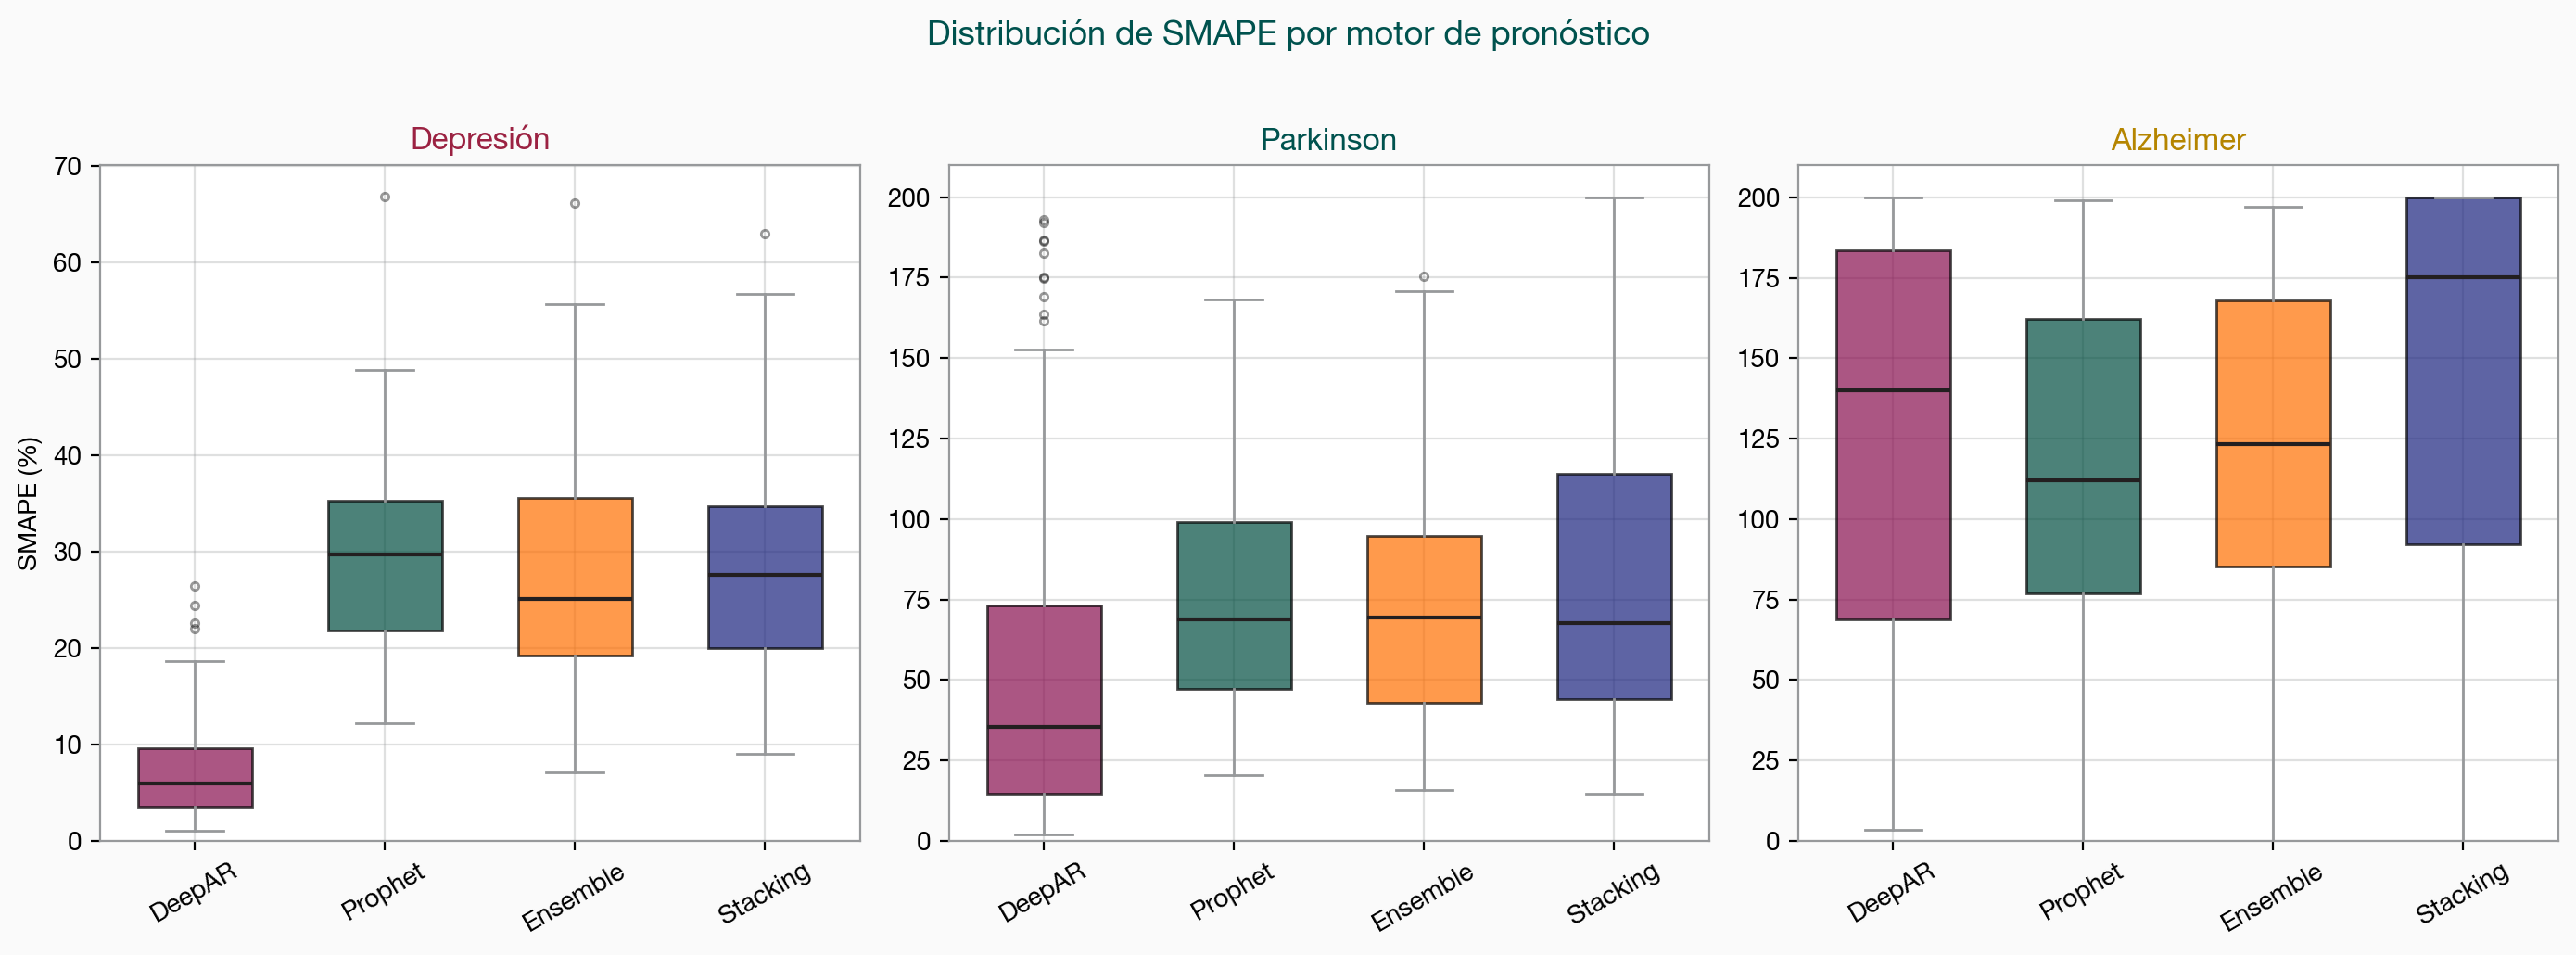
\includegraphics[width=0.95\textwidth]{fig_boxplot_smape_motores.png}
\caption[Box plot de SMAPE por motor.]{Distribución de \smape{} por motor de pronóstico, faceteado por padecimiento. DeepAR presenta medianas consistentemente más bajas y menor dispersión.}
\label{fig:boxplot_motores}
\end{figure}

\begin{figure}[H]
\centering
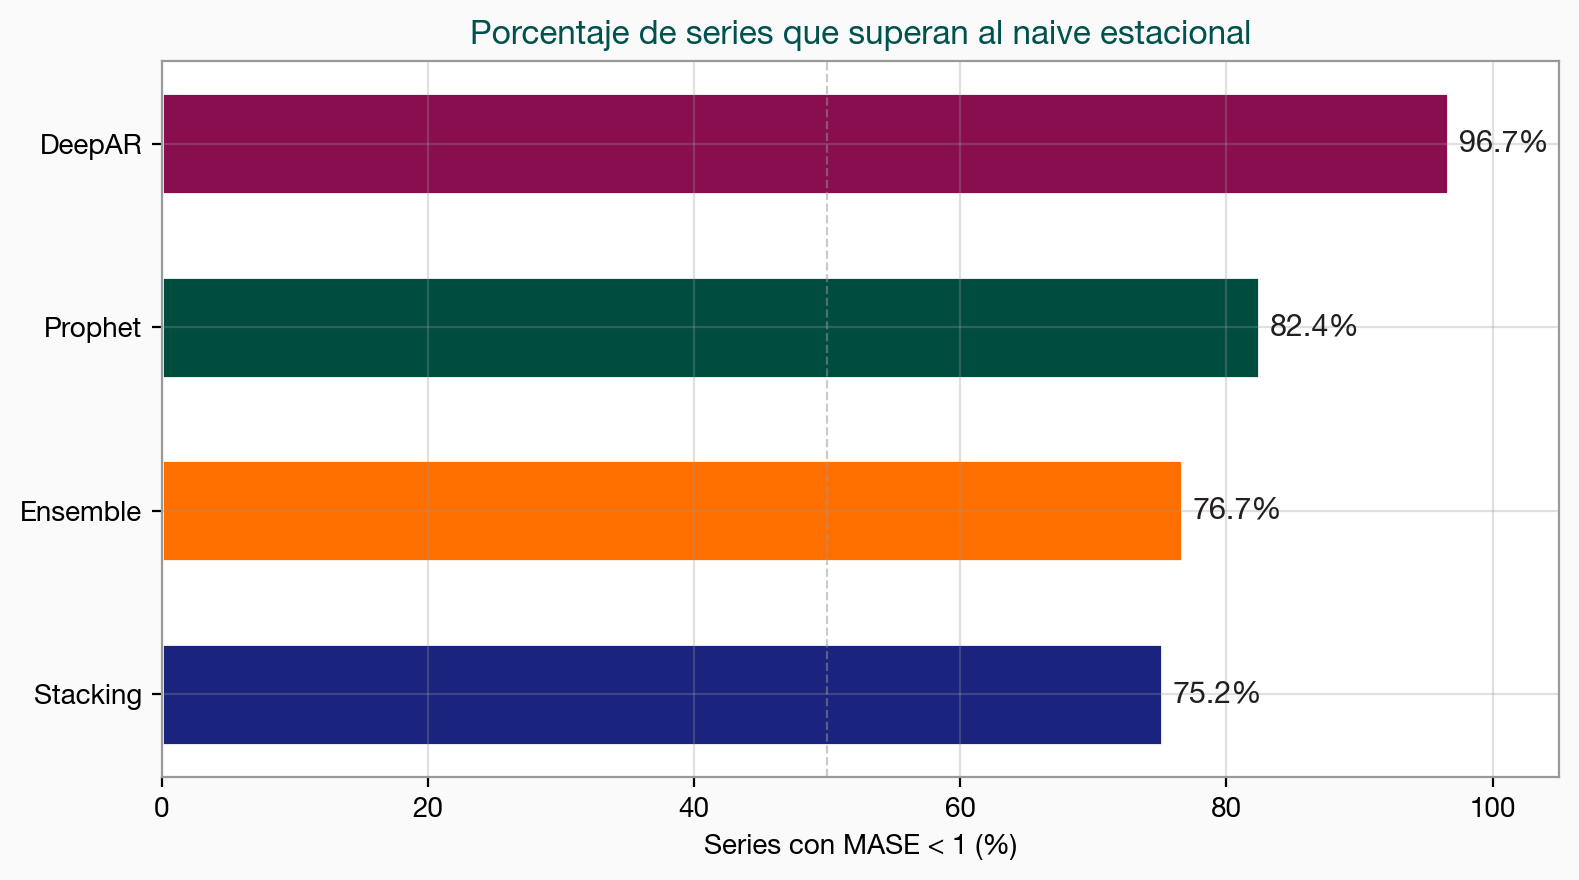
\includegraphics[width=0.75\textwidth]{fig_barras_mase_motores.png}
\caption[Comparativa de MASE por motor.]{Porcentaje de series donde el modelo supera al naive estacional (\mase{} $<$ 1) por motor.}
\label{fig:barras_mase}
\end{figure}

\begin{championbox}[ Depresión (F32)]
\textbf{Motor}: \textcolor{cdeepar}{DeepAR} gana 108 de 111 series (97.3\%). \\
\textbf{\smape{} mediano}: 5.99\% \quad \textbf{\mase{} mediano}: 0.17 \\
\textbf{Pronóstico Nacional (general) a 52 semanas}: 155,966 casos.
\end{championbox}

\begin{championbox}[ Parkinson (G20)]
\textbf{Motor}: \textcolor{cdeepar}{DeepAR} gana 89 de 111 series (80.2\%). \\
\textbf{\smape{} mediano}: 35.24\% \quad \textbf{\mase{} mediano}: 0.26 \\
\textbf{Pronóstico Nacional (general) a 52 semanas}: 8,234 casos.
\end{championbox}

\begin{championbox}[ Alzheimer (G30)]
\textbf{Motor}: \textcolor{cdeepar}{DeepAR} gana 47 de 111 series (42.3\%). \\
\textbf{\smape{} mediano}: 107.59\% \quad \textbf{\mase{} mediano}: 0.63 \\
\textbf{Pronóstico Nacional (general) a 52 semanas}: 1,249 casos.
\end{championbox}

\subsection{Semáforo de calidad por estado}

La \tabref{tab:semaforo} clasifica los estados según la calidad del pronóstico de Depresión, mientras que la \figref{fig:mapa_smape} ofrece una perspectiva geográfica de esta métrica.

\begin{figure}[H]
\centering
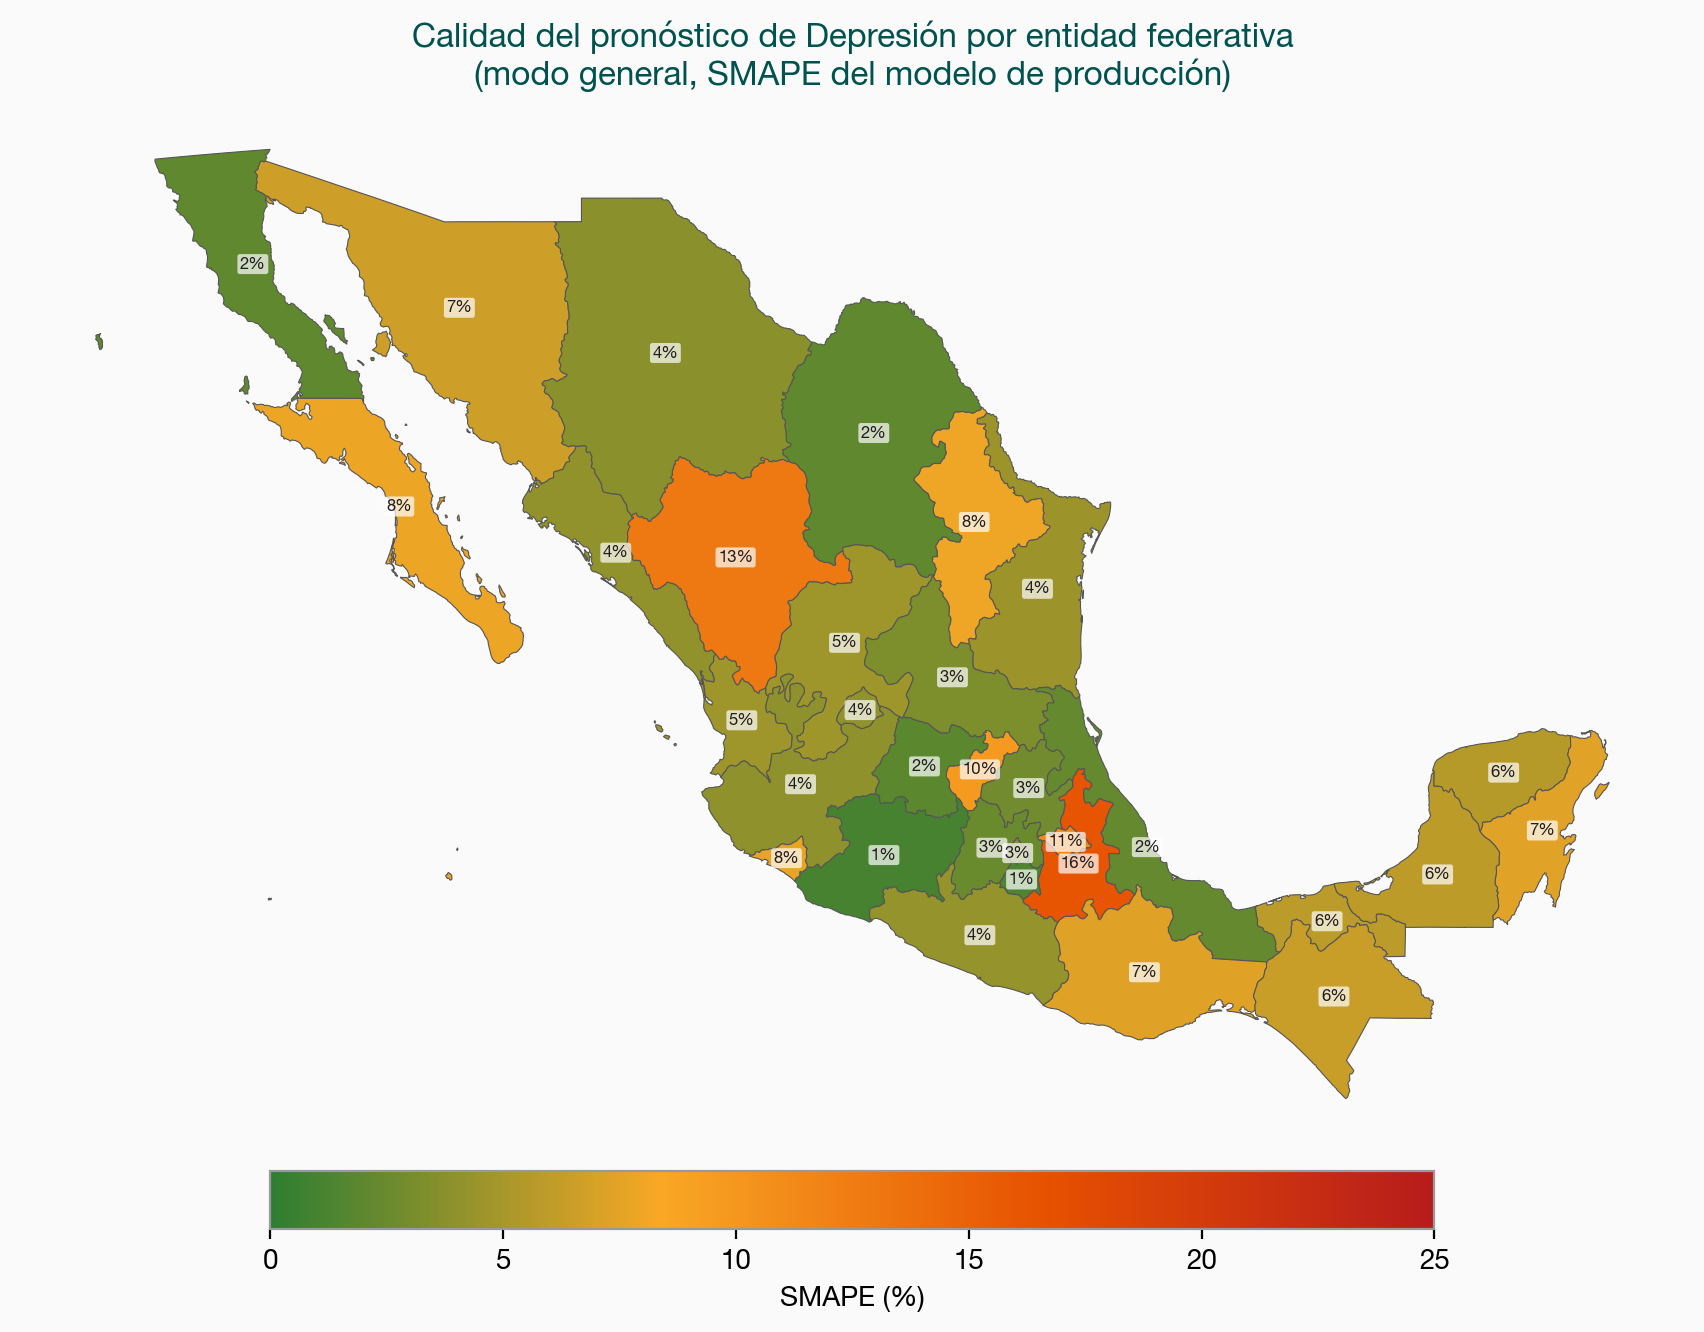
\includegraphics[width=0.85\textwidth]{fig_mapa_smape_depresion.png}
\caption[Mapa semáforo de SMAPE (Depresión).]{Calidad del pronóstico por entidad federativa. Los estados con mayor volumen obtienen consistentemente mejores resultados.}
\label{fig:mapa_smape}
\end{figure}

\begin{table}[H]
\centering
\caption{Semáforo de calidad del pronóstico de Depresión por entidad (top 10 y bottom 5)}
\label{tab:semaforo}
\scriptsize
\setlength{\tabcolsep}{4pt}
\begin{tabular}{cl rr cl rr}
\toprule
& \multicolumn{3}{c}{\textbf{Top 10 (menor \smape{})}} & & \multicolumn{3}{c}{\textbf{Bottom 5 (mayor \smape{})}} \\
\cmidrule(lr){2-4} \cmidrule(lr){6-8}
& \textbf{Entidad} & \smape{} & \mase{} & & \textbf{Entidad} & \smape{} & \mase{} \\
\midrule
\cellcolor{lightgreen} & Michoacán & 1.0\% & 0.05 & \cellcolor{lightred} & Puebla & 16.3\% & 0.42 \\
\cellcolor{lightgreen} & Morelos & 1.4\% & 0.04 & \cellcolor{lightred} & Durango & 12.9\% & 0.41 \\
\cellcolor{lightgreen} & Guanajuato & 1.9\% & 0.08 & \cellcolor{lightred} & Reg.\ Sur-Sureste & 11.5\% & 0.69 \\
\cellcolor{lightgreen} & Baja California & 2.1\% & 0.09 & \cellcolor{lightred} & Tlaxcala & 11.5\% & 0.37 \\
\cellcolor{lightgreen} & Coahuila & 2.1\% & 0.05 & \cellcolor{lightred} & Querétaro & 9.7\% & 0.30 \\
\cellcolor{lightgreen} & Veracruz & 2.3\% & 0.08 & & & & \\
\cellcolor{lightgreen} & México & 2.5\% & 0.09 & & & & \\
\cellcolor{lightgreen} & Hidalgo & 2.8\% & 0.11 & & & & \\
\cellcolor{lightgreen} & San Luis Potosí & 3.3\% & 0.09 & & & & \\
\cellcolor{lightgreen} & Ciudad de México & 3.5\% & 0.16 & & & & \\
\bottomrule
\end{tabular}
\end{table}

La disparidad en la dificultad de modelado entre padecimientos se visualiza en el \figref{fig:heatmap_smape}, donde Alzheimer presenta los mayores retos métricos de forma generalizada.

\begin{figure}[H]
\centering
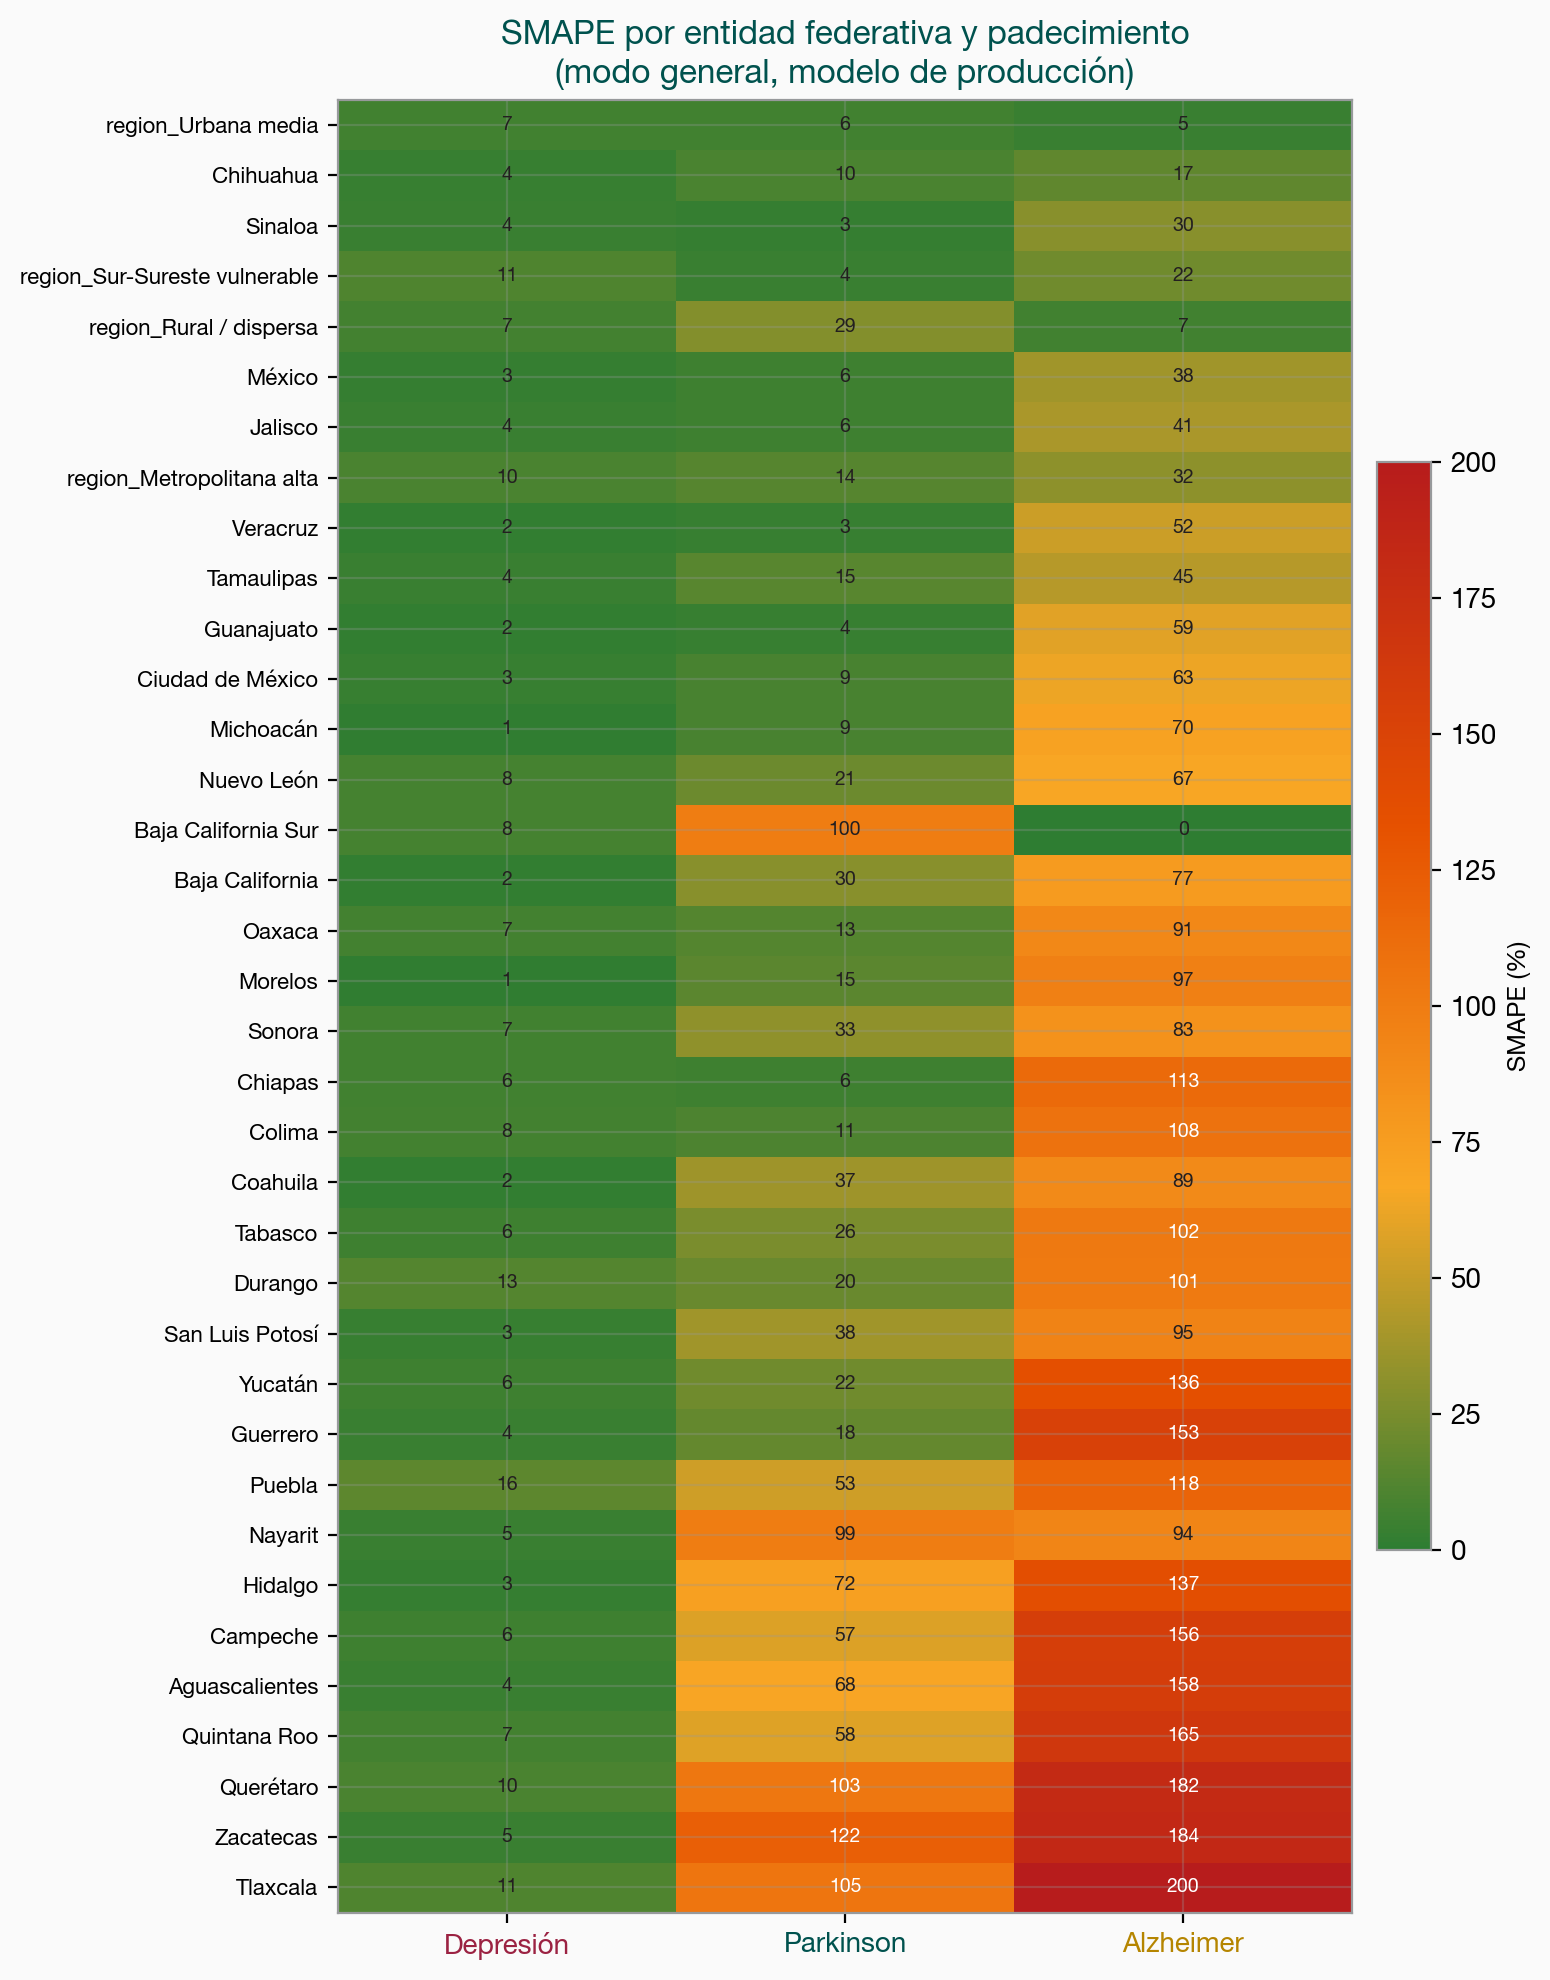
\includegraphics[width=0.95\textwidth]{fig_heatmap_smape_estado_pad.png}
\caption[Heatmap de SMAPE por estado y padecimiento.]{La intensidad del color refleja el nivel de error; Alzheimer presenta los valores más altos en todas las entidades.}
\label{fig:heatmap_smape}
\end{figure}

\begin{insightbox}[Patrón claro: volumen = precisión]
Los estados con mayor y más estable volumen de consultas (Michoacán, Morelos, Guanajuato, Baja California, Coahuila) obtienen los mejores \smape{}. Esto es consistente con el hecho de que series con mayor incidencia presentan menor varianza relativa, lo que facilita el aprendizaje del modelo. Por el contrario, estados con menor volumen o alta variabilidad (Puebla, Durango, Tlaxcala) muestran mayor ruido proporcional.
\end{insightbox}

\subsection{Análisis por sexo}

El desglose por sexo (Masculino, Femenino y Combinado) revela patrones diferenciados:

\begin{itemize}[noitemsep]
    \item \textbf{Depresión}: las mujeres representan $\approx$70\% de los casos, consistente con la prevalencia global reportada por la OMS (s.\,f.). Los modelos para el sexo femenino alcanzan mejor \smape{} que los masculinos (menor varianza relativa por mayor volumen).
    \item \textbf{Parkinson}: distribución más equilibrada ($\approx$55\% hombres). Los modelos por sexo tienen precisión similar.
    \item \textbf{Alzheimer}: ligero predominio femenino ($\approx$58\%). Patrones estables sin diferencias significativas entre sexos.
\end{itemize}

Como se visualiza en la \figref{fig:distribucion_sexo}, la composición demográfica de la incidencia varía drásticamente según el padecimiento.

\begin{figure}[H]
\centering
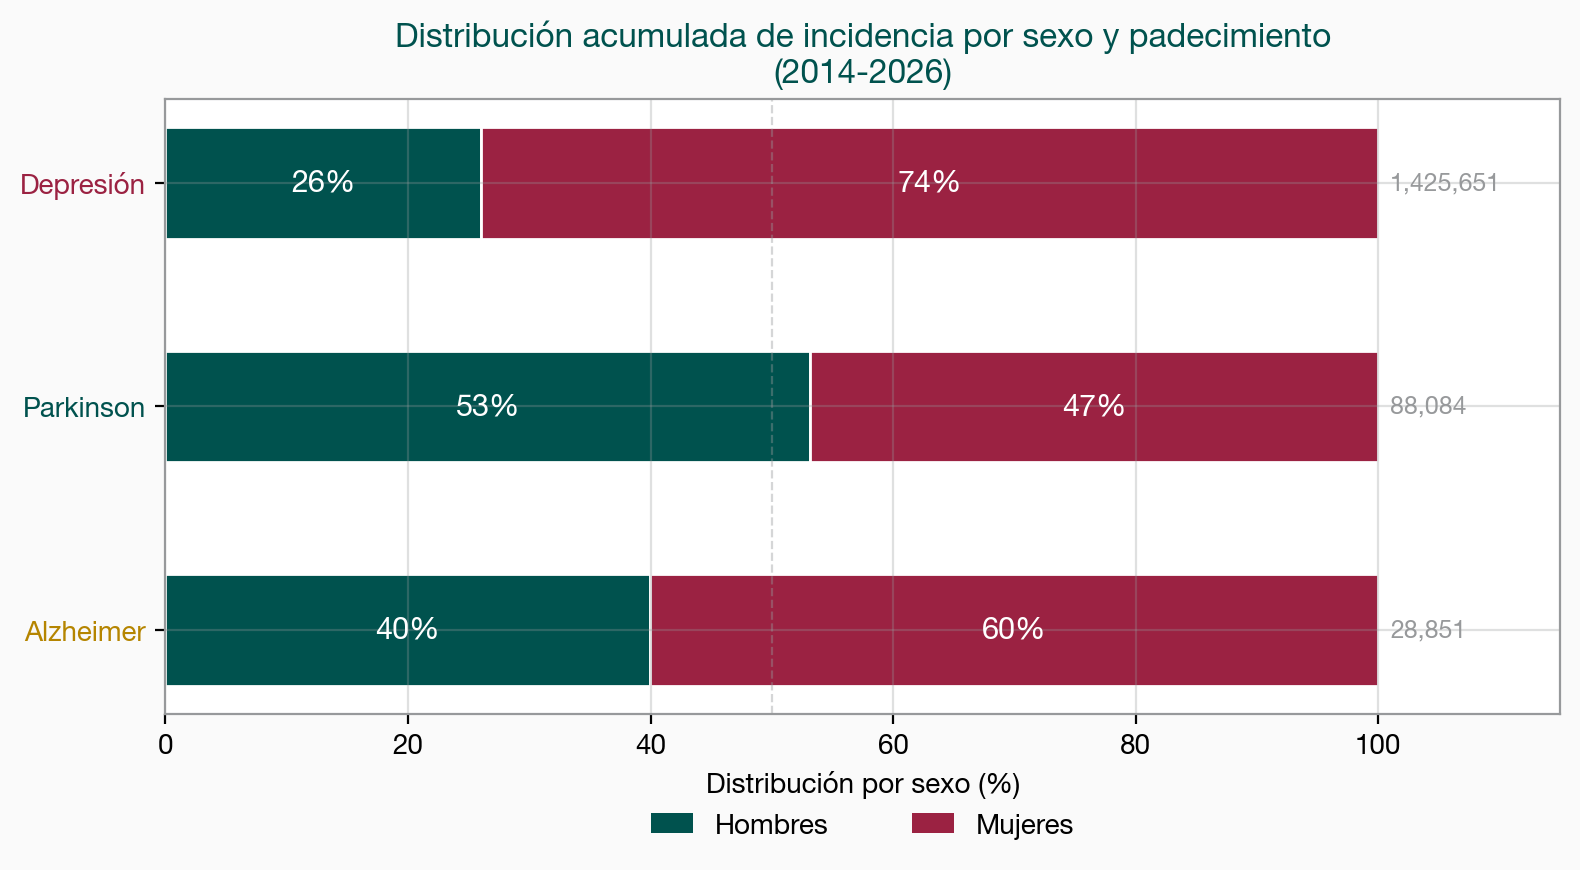
\includegraphics[width=0.70\textwidth]{fig_distribucion_sexo.png}
\caption[Distribución de incidencia por sexo.]{Distribución acumulada por sexo; Depresión muestra un marcado predominio femenino ($\approx$70\%).}
\label{fig:distribucion_sexo}
\end{figure}

\subsection{Impacto de COVID-19}

La pandemia de COVID-19 (2020\,--\,2022) coincide temporalmente con un \textbf{quiebre observable} en las series de Depresión, con una caída abrupta durante el periodo de confinamiento seguida de un incremento sostenido. El modelo Prophet, según Taylor y Letham (2018), manejó este quiebre mediante changepoints explícitos, mientras que DeepAR lo aprendió implícitamente a través de su ventana de contexto (Salinas et al., 2020).

Para Parkinson y Alzheimer, el impacto fue moderado: una reducción temporal en el registro de casos, potencialmente asociada con menor utilización de servicios y cambios en la captación, seguida de una recuperación gradual. En la \figref{fig:covid_impact} se observa este fenómeno para el caso de Depresión.

\begin{figure}[H]
\centering
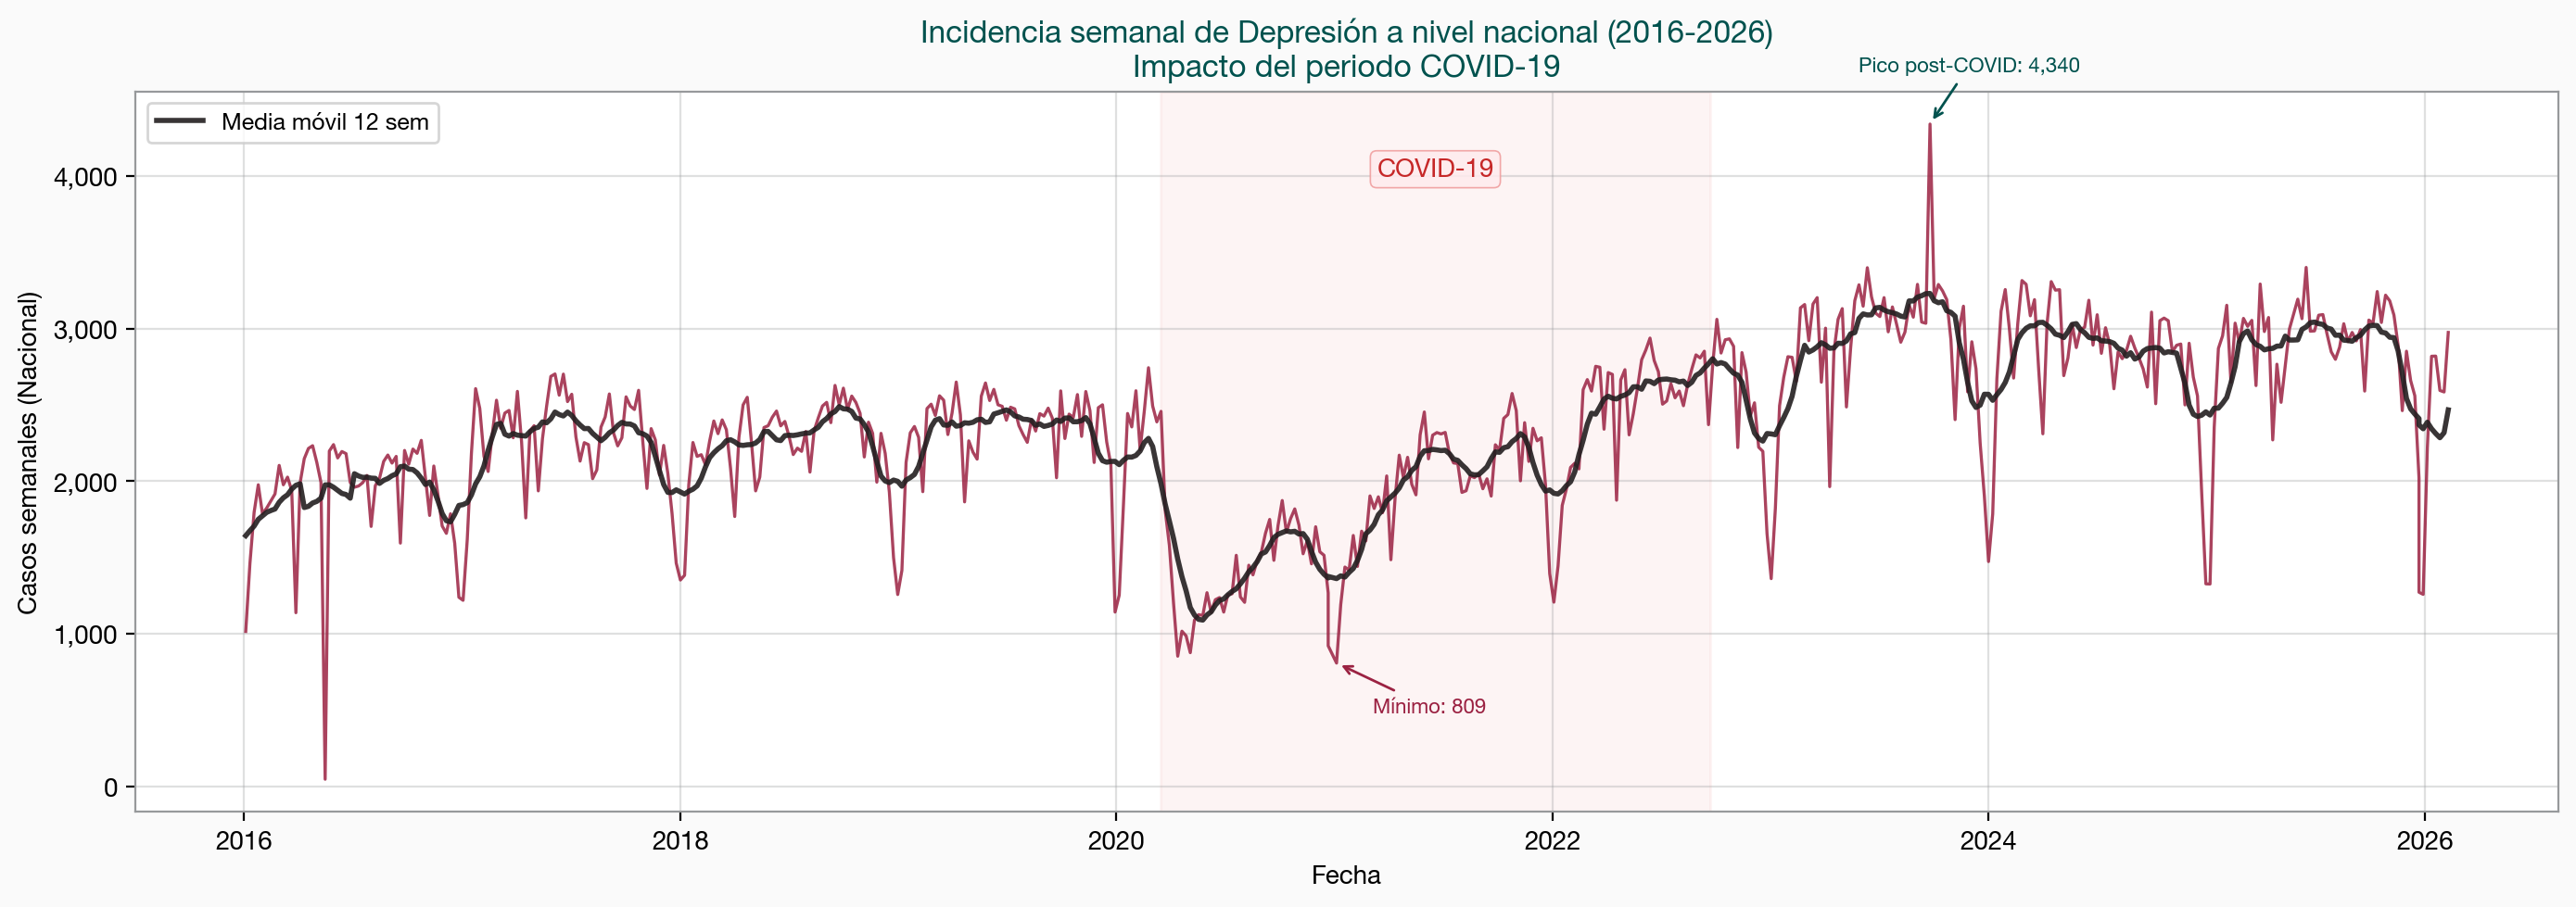
\includegraphics[width=0.95\textwidth]{fig_covid_impact_depresion.png}
\caption[Impacto de COVID-19 en Depresión.]{Incidencia semanal nacional (2016--2026) con el periodo COVID-19 (marzo 2020 -- septiembre 2022) sombreado en rojo, mostrando la caída abrupta y el rebote sostenido.}
\label{fig:covid_impact}
\end{figure}

\subsection{Diagnósticos de calidad}

\begin{table}[H]
\centering
\caption{Diagnósticos de overfitting y leakage en los 333 modelos de producción}
\label{tab:diagnosticos}
\small
\begin{tabularx}{\textwidth}{l r X}
\toprule
\textbf{Diagnóstico} & \textbf{Modelos} & \textbf{Descripción} \\
\midrule
\multicolumn{3}{l}{\textit{Overfitting (ratio \smape{} test / \smape{} train)}} \\
OK ($<$1.3$\times$) & 328 & Sin evidencia de sobreajuste \\
Moderado (1.3\,--\,2$\times$) & 1 & Monitorear en próximas iteraciones \\
Alto ($>$2$\times$) & 1 & Reentrenar con regularización adicional \\
N/D & 3 & Series con train \smape{} = 0 (indivisible) \\
\midrule
\multicolumn{3}{l}{\textit{Leakage (\smape{} train $<$ 0.5\%)}} \\
OK & 330 & Sin fuga de datos detectada \\
Sospechoso & 3 & \smape{} train anormalmente bajo; revisar features \\
\bottomrule
\end{tabularx}
\end{table}

\begin{insightbox}[Integridad del pipeline]
La tasa de modelos saludables (OK en ambos diagnósticos) es del \textbf{98.5\%} (328/333). Los 5 modelos con alertas incluyen 4 series de Alzheimer con incidencia $<$2 casos/semana (3 de BCS con overfitting N/D y leakage sospechoso, 1 de CDMX con overfitting moderado) y 1 serie de Depresión Nacional hombres con overfitting alto (2.0$\times$).
\end{insightbox}

\newpage
% =============================================================================
% 6. VALIDACION SEMANAL CON DATOS REALES
% =============================================================================
\section{Validación Semanal con Datos Reales}\label{sec:validacion}

\subsection{El experimento definitivo}

Una vez seleccionados los modelos de producción, se realizó una validación genuinamente \textit{out-of-sample}: se compararon los pronósticos generados \textbf{antes} de la publicación del boletín SINAVE (Secretaría de Salud, 2025) de la semana epidemiológica más reciente contra los datos reales que los modelos \textbf{nunca vieron} durante el entrenamiento ni la validación cruzada.

\begin{insightbox}[Validación out-of-sample genuina]
Esta validación semanal es el estándar de oro para evaluar un sistema de pronóstico en producción. Los datos reales provienen del boletín SINAVE publicado \textit{después} del entrenamiento. Ningún modelo tuvo acceso a estos valores durante el ajuste de hiperparámetros, la selección de features ni la validación cruzada.
\end{insightbox}

\subsection{Protocolo de validación}

\begin{enumerate}[noitemsep]
    \item Los 333 modelos de producción generan pronósticos para la semana $t+1$.
    \item Se publica el boletín SINAVE correspondiente a la semana $t+1$.
    \item Se compara \texttt{pron\_sem\_previa} (pronóstico) contra \texttt{realidad\_sem\_previa} (dato real).
    \item Se calcula el error absoluto y porcentual por serie.
    \item Los resultados se publican automáticamente en \texttt{validacion\_semanal.html}.
\end{enumerate}

La tabla de producción (\texttt{tabla\_333\_modelos\_produccion.xlsx}) incluye dos columnas dedicadas a esta validación:
\begin{itemize}[noitemsep]
    \item \texttt{pron\_sem\_previa}: predicción del modelo para la semana más reciente.
    \item \texttt{realidad\_sem\_previa}: dato real del boletín SINAVE.
\end{itemize}

Adicionalmente, la comparativa histórica incluye:
\begin{itemize}[noitemsep]
    \item \texttt{casos\_prev\_52\_semanas\_real}: casos reales en las últimas 52 semanas.
    \item \texttt{casos\_prev\_52\_semanas\_pronos}: pronóstico acumulado para el mismo periodo.
    \item \texttt{precision\_historica}: ratio pronóstico/real como porcentaje.
\end{itemize}

El seguimiento de estas métricas se realiza mediante reportes automatizados publicados en el sitio web del proyecto, como se ilustra en la \figref{fig:validacion_screenshot}. El reporte completo está disponible en \url{https://proyectointegrador.org/validacion_semanal}.

\begin{figure}[H]
\centering
\makebox[\textwidth][c]{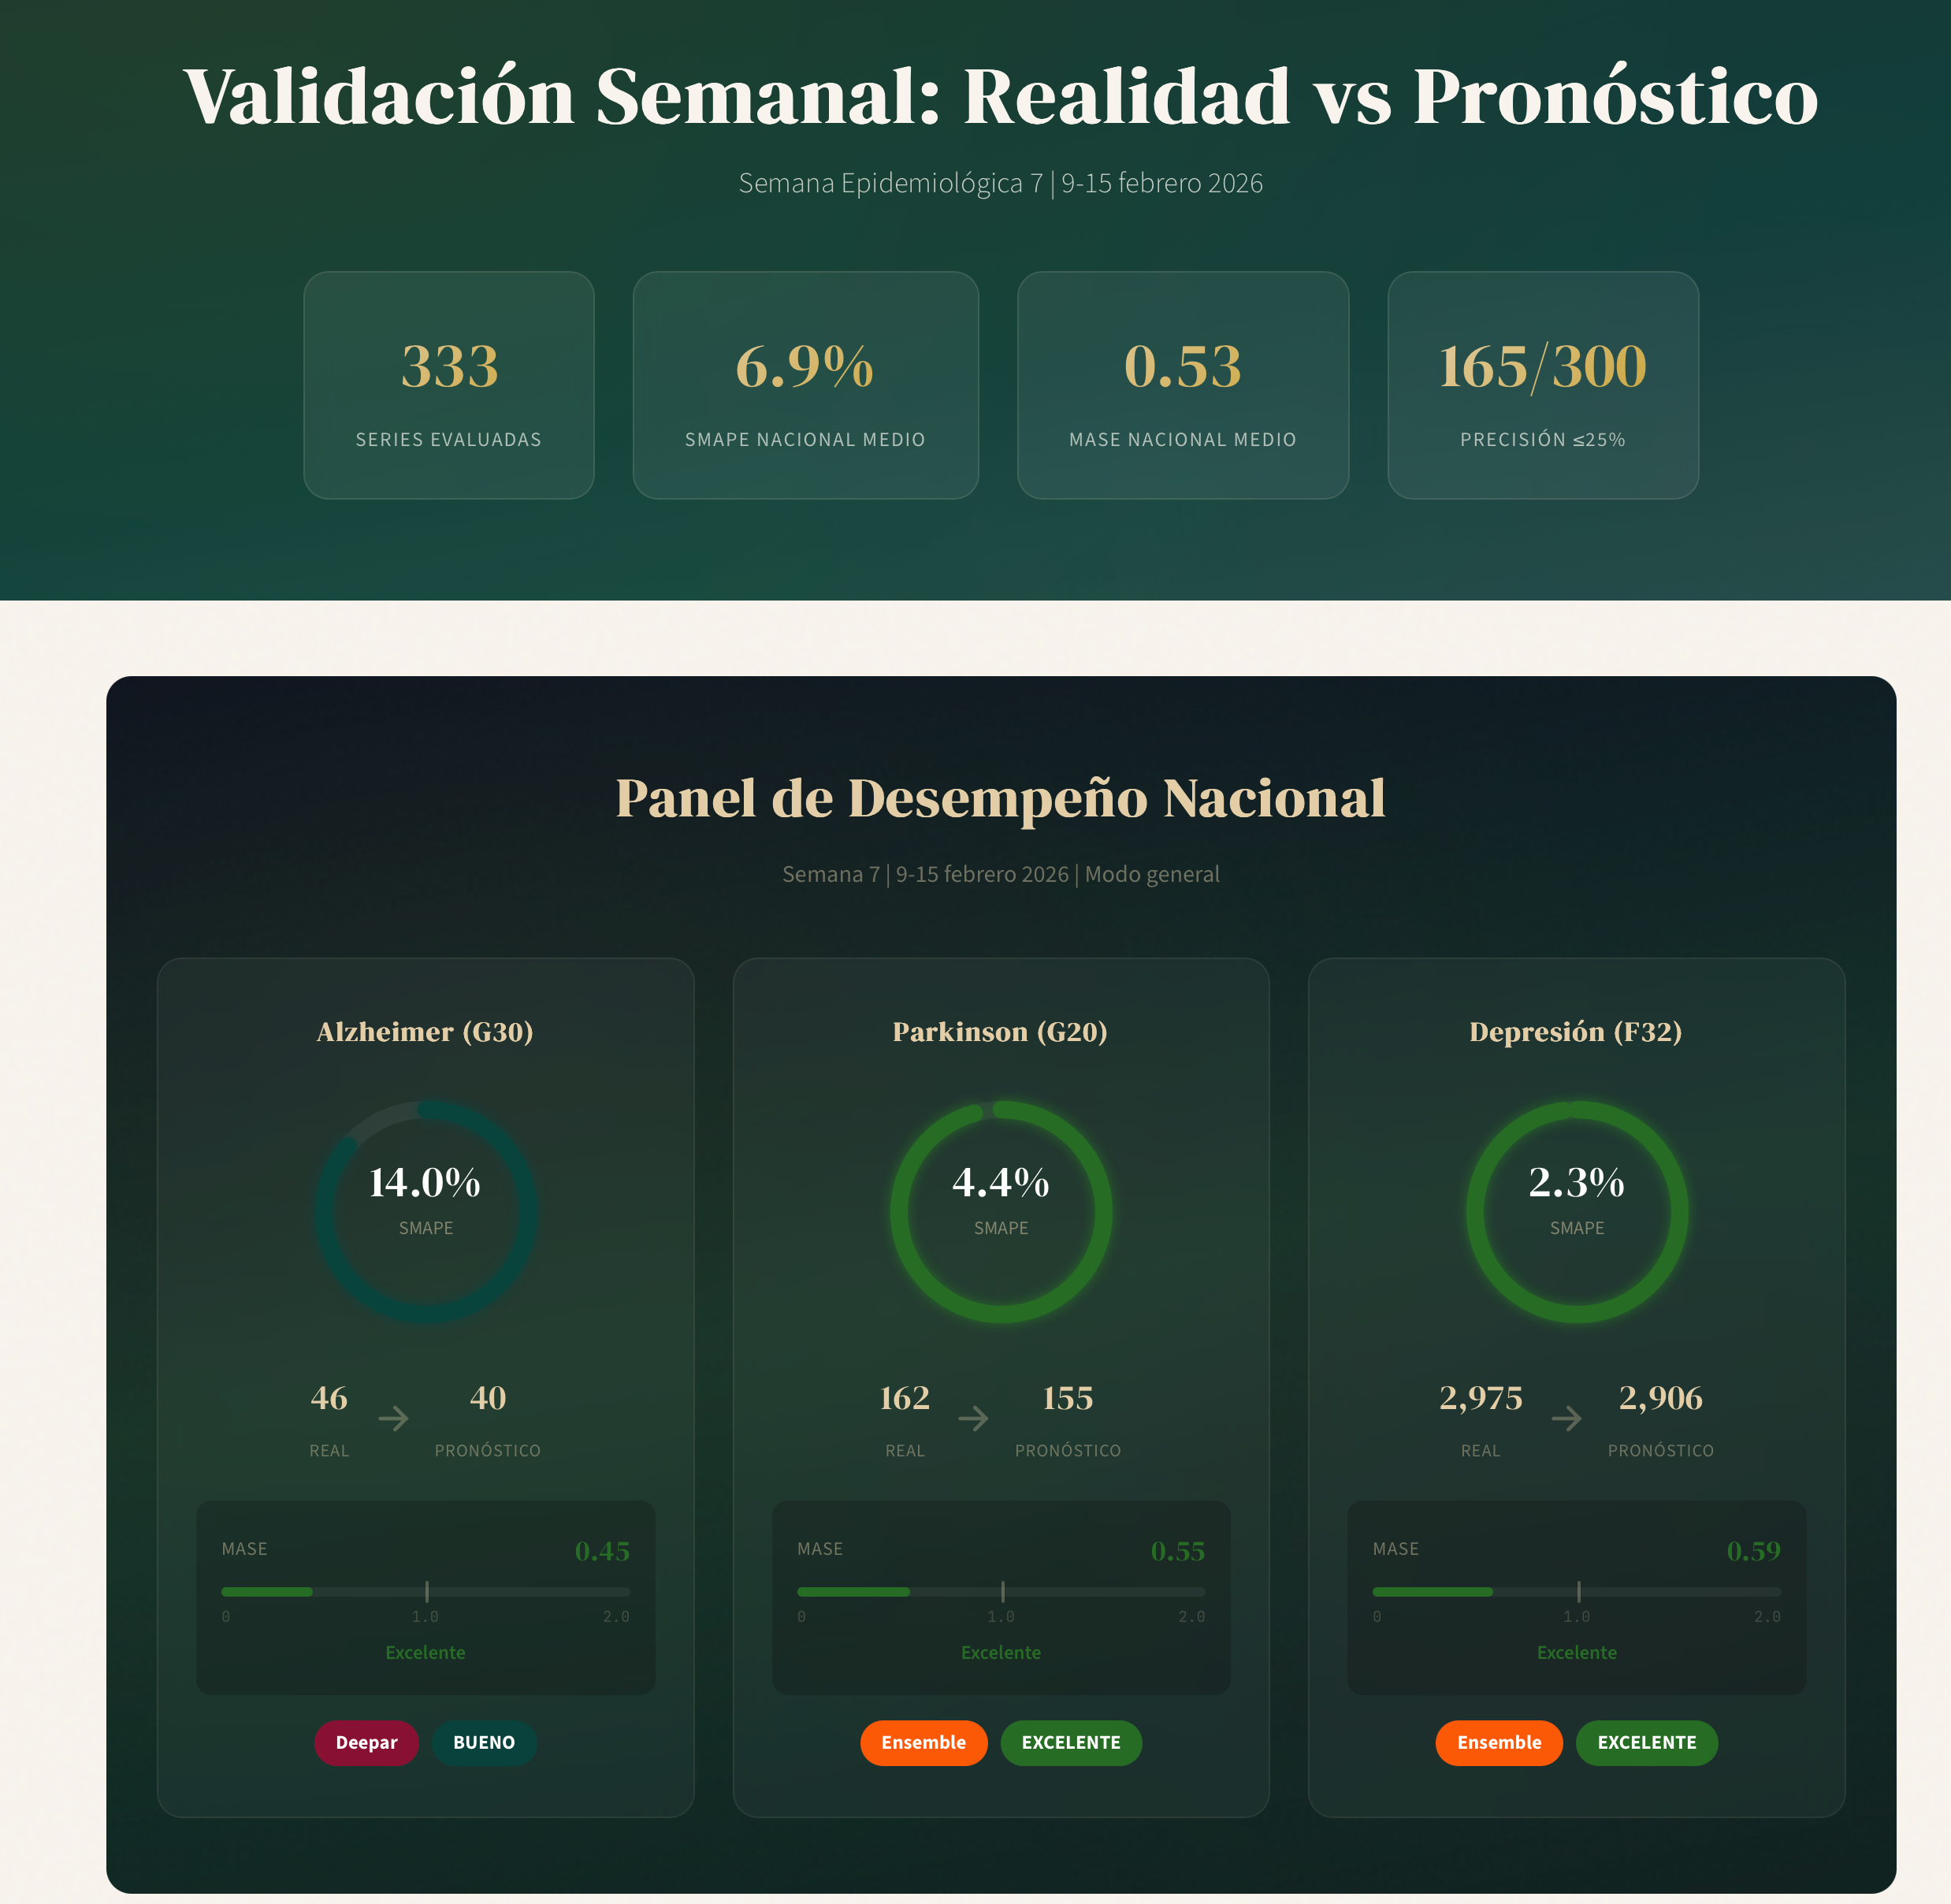
\includegraphics[width=1.15\textwidth]{screenshot_validacion_semanal.png}}
\caption[Reporte de validación semanal.]{Extracto del reporte de validación semanal publicado en \url{https://proyectointegrador.org/validacion_semanal}, comparando pronóstico vs realidad para la semana epidemiológica más reciente.}
\label{fig:validacion_screenshot}
\end{figure}

\newpage
% =============================================================================
% 7. CONCLUSIONES POR PADECIMIENTO
% =============================================================================
\section{Conclusiones por Padecimiento}\label{sec:conclusiones_pad}

\subsection{Depresión (F32)}\label{subsec:depresion}

\subsubsection{Insights epidemiológicos}

La Depresión es el padecimiento con mayor volumen de incidencia entre los tres estudiados, con un pronóstico de \textbf{155,966 casos} a nivel nacional (general) para las próximas 52 semanas. Este volumen permite a los modelos capturar patrones robustos con alta precisión.

\begin{itemize}[noitemsep]
    \item \textbf{Tendencia}: ascendente sostenida desde 2021 (post-COVID), con un incremento anual del $\approx$12\%.
    \item \textbf{Estacionalidad}: pico en octubre y noviembre, consistente con un patrón estacional de mayor demanda observado en la serie; esta asociación temporal no debe interpretarse por sí sola como evidencia etiológica. Valle en febrero y marzo.
    \item \textbf{COVID-19}: caída abrupta en 2020 durante el periodo de confinamiento, seguida de un rebote que superó los niveles pre-pandémicos, consistente con la literatura internacional (OMS, s.\,f.).
\end{itemize}

Esta dinámica se refleja en el pronóstico nacional presentado en la \figref{fig:forecast_depresion}.

\begin{figure}[H]
\centering
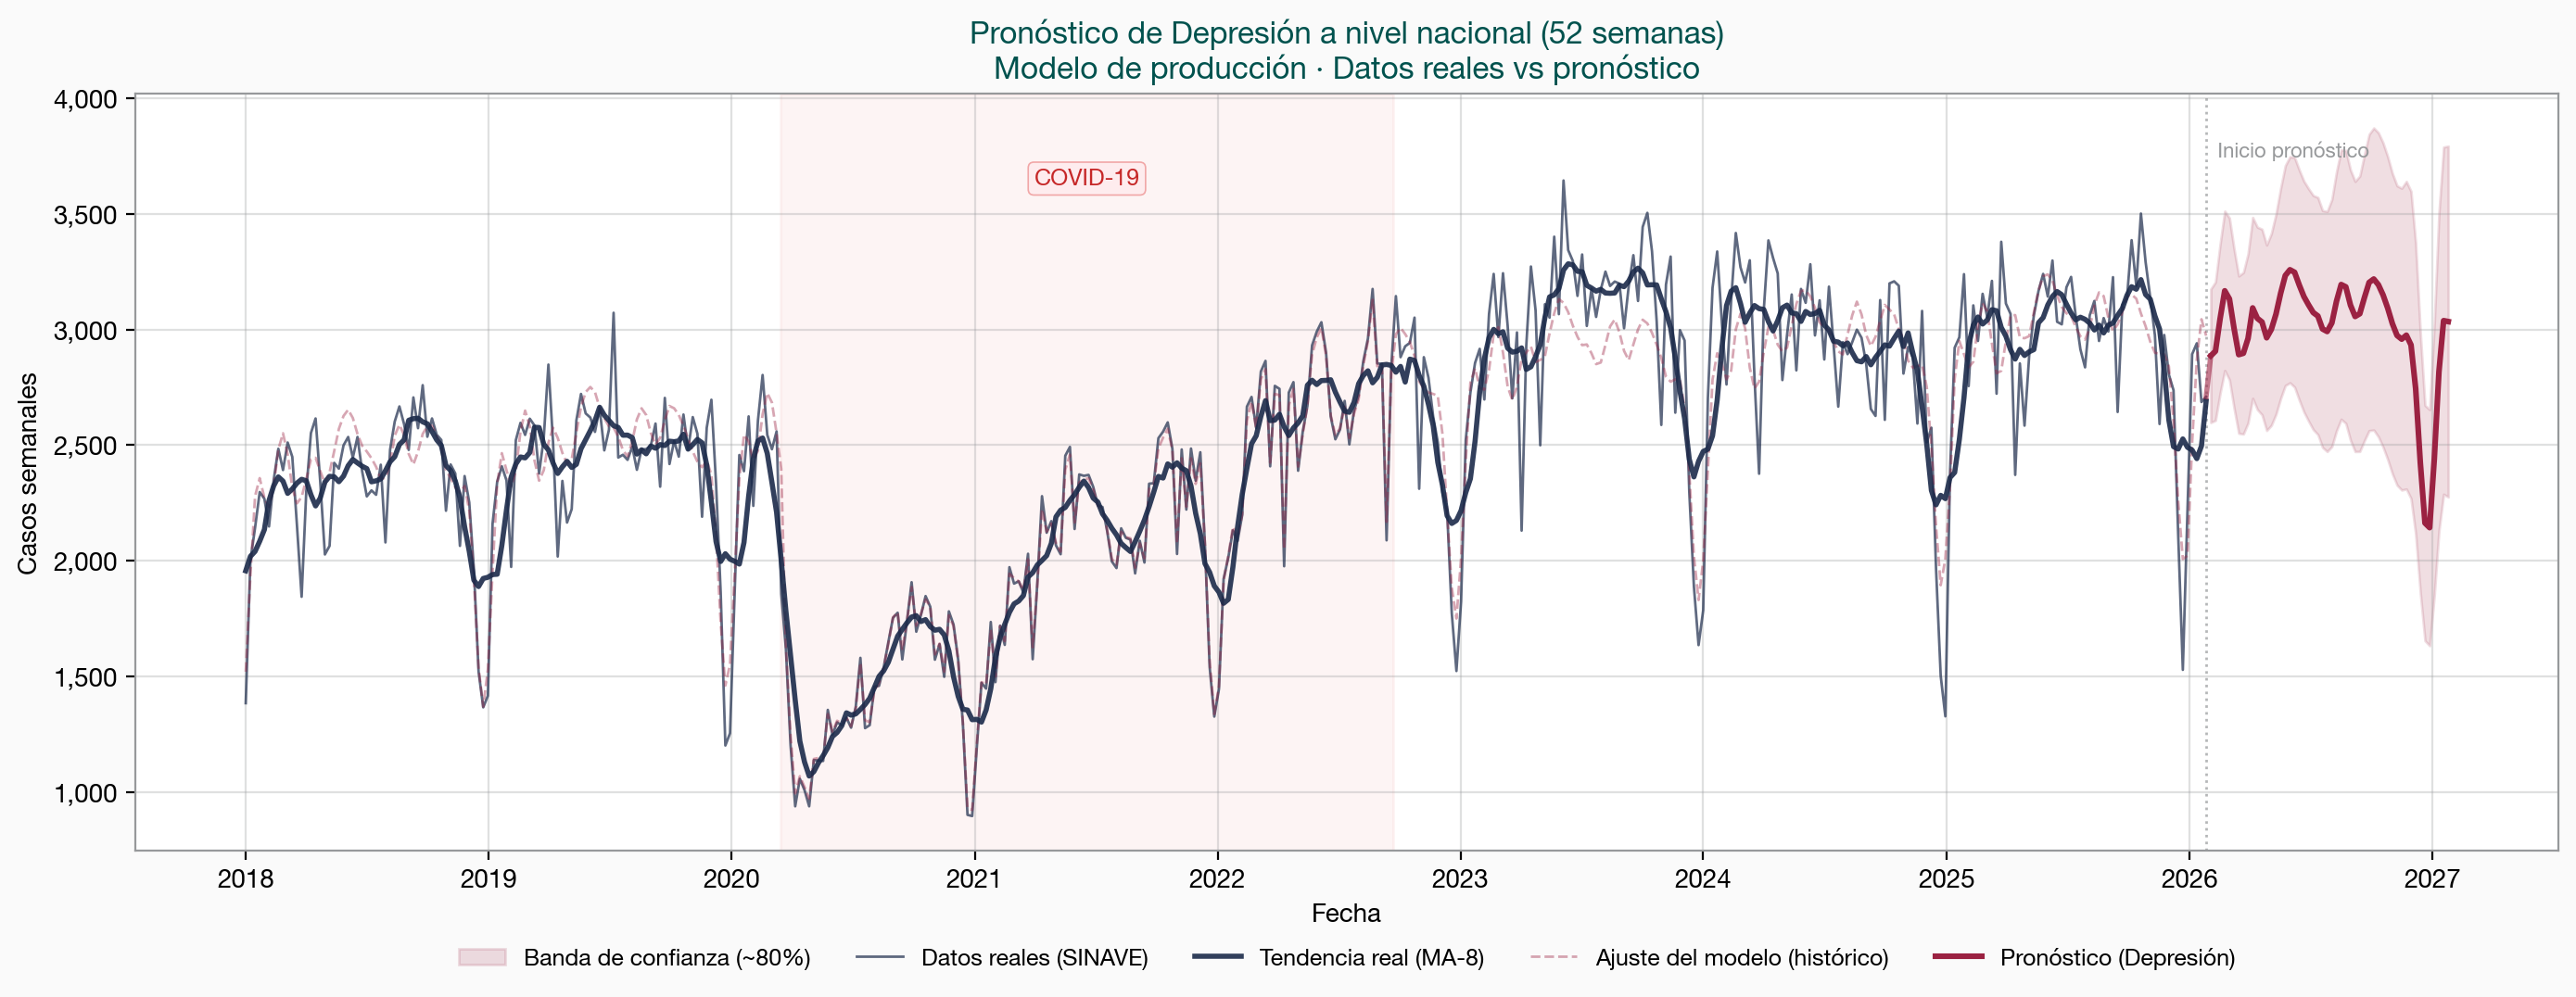
\includegraphics[width=0.95\textwidth]{fig_forecast_depresion_nacional.png}
\caption[Pronóstico de Depresión Nacional.]{Serie real (azul oscuro) vs pronóstico a 52 semanas (guinda) con banda de confianza al $\sim$80\%, correspondiente a la serie nacional para la cual el motor seleccionado en producción fue Ensemble. La línea punteada muestra el ajuste histórico. Franja roja: periodo COVID-19 (marzo 2020 -- septiembre 2022).}

\label{fig:forecast_depresion}
\end{figure}

\subsubsection{Mejores y peores estados}

\begin{itemize}[noitemsep]
    \item \textbf{Mejores} (menor \smape{}): Michoacán, Morelos, Guanajuato, Baja California, Coahuila. Estados con series estables y volumen suficiente.
    \item \textbf{Peores} (mayor \smape{}): Puebla, Durango, Tlaxcala, Querétaro. Estados con alta variabilidad relativa en sus series.
\end{itemize}

\subsubsection{Diferencial por sexo}

Las mujeres representan $\approx$70\% de los diagnósticos de Depresión, alineado con la prevalencia global reportada por la OMS (s.\,f.). Los modelos femeninos alcanzan mejor \smape{} (menor varianza relativa) que los masculinos. Recomendación: el {\imss} debe considerar programas diferenciados de detección temprana con énfasis en la población femenina.

\subsubsection{Implicaciones clínicas}

\begin{enumerate}[noitemsep]
    \item \textbf{Planificación de medicamentos}: los pronósticos permiten anticipar la demanda de antidepresivos (ISRS, IRSN) por estado y sexo.
    \item \textbf{Recursos humanos}: estados con tendencia ascendente deben ampliar la plantilla de psicólogos y psiquiatras.
    \item \textbf{Campañas de prevención}: los picos estacionales sugieren intensificar las campañas de salud mental en septiembre y octubre, antes del pico.
\end{enumerate}

\subsection{Parkinson (G20)}\label{subsec:parkinson}

\subsubsection{Insights epidemiológicos}

Parkinson presenta un pronóstico de \textbf{8,234 casos} a nivel nacional (general) en 52 semanas, con una incidencia mucho menor que Depresión. La serie es relativamente estable, con estacionalidad suave y tendencia ligeramente ascendente asociada al envejecimiento poblacional (INEGI, 2024).

\begin{itemize}[noitemsep]
    \item \textbf{Tendencia}: levemente ascendente ($\approx$3\% anual), compatible con el envejecimiento de la pirámide poblacional mexicana.
    \item \textbf{Estacionalidad}: débil; ligeros picos en marzo y abril, posiblemente asociados con consultas de seguimiento post-invernal.
    \item \textbf{COVID-19}: impacto moderado; reducción temporal por caída en consultas presenciales, recuperación gradual en 2022.
\end{itemize}

El pronóstico para este padecimiento se visualiza en la \figref{fig:forecast_parkinson}.

\begin{figure}[H]
\centering
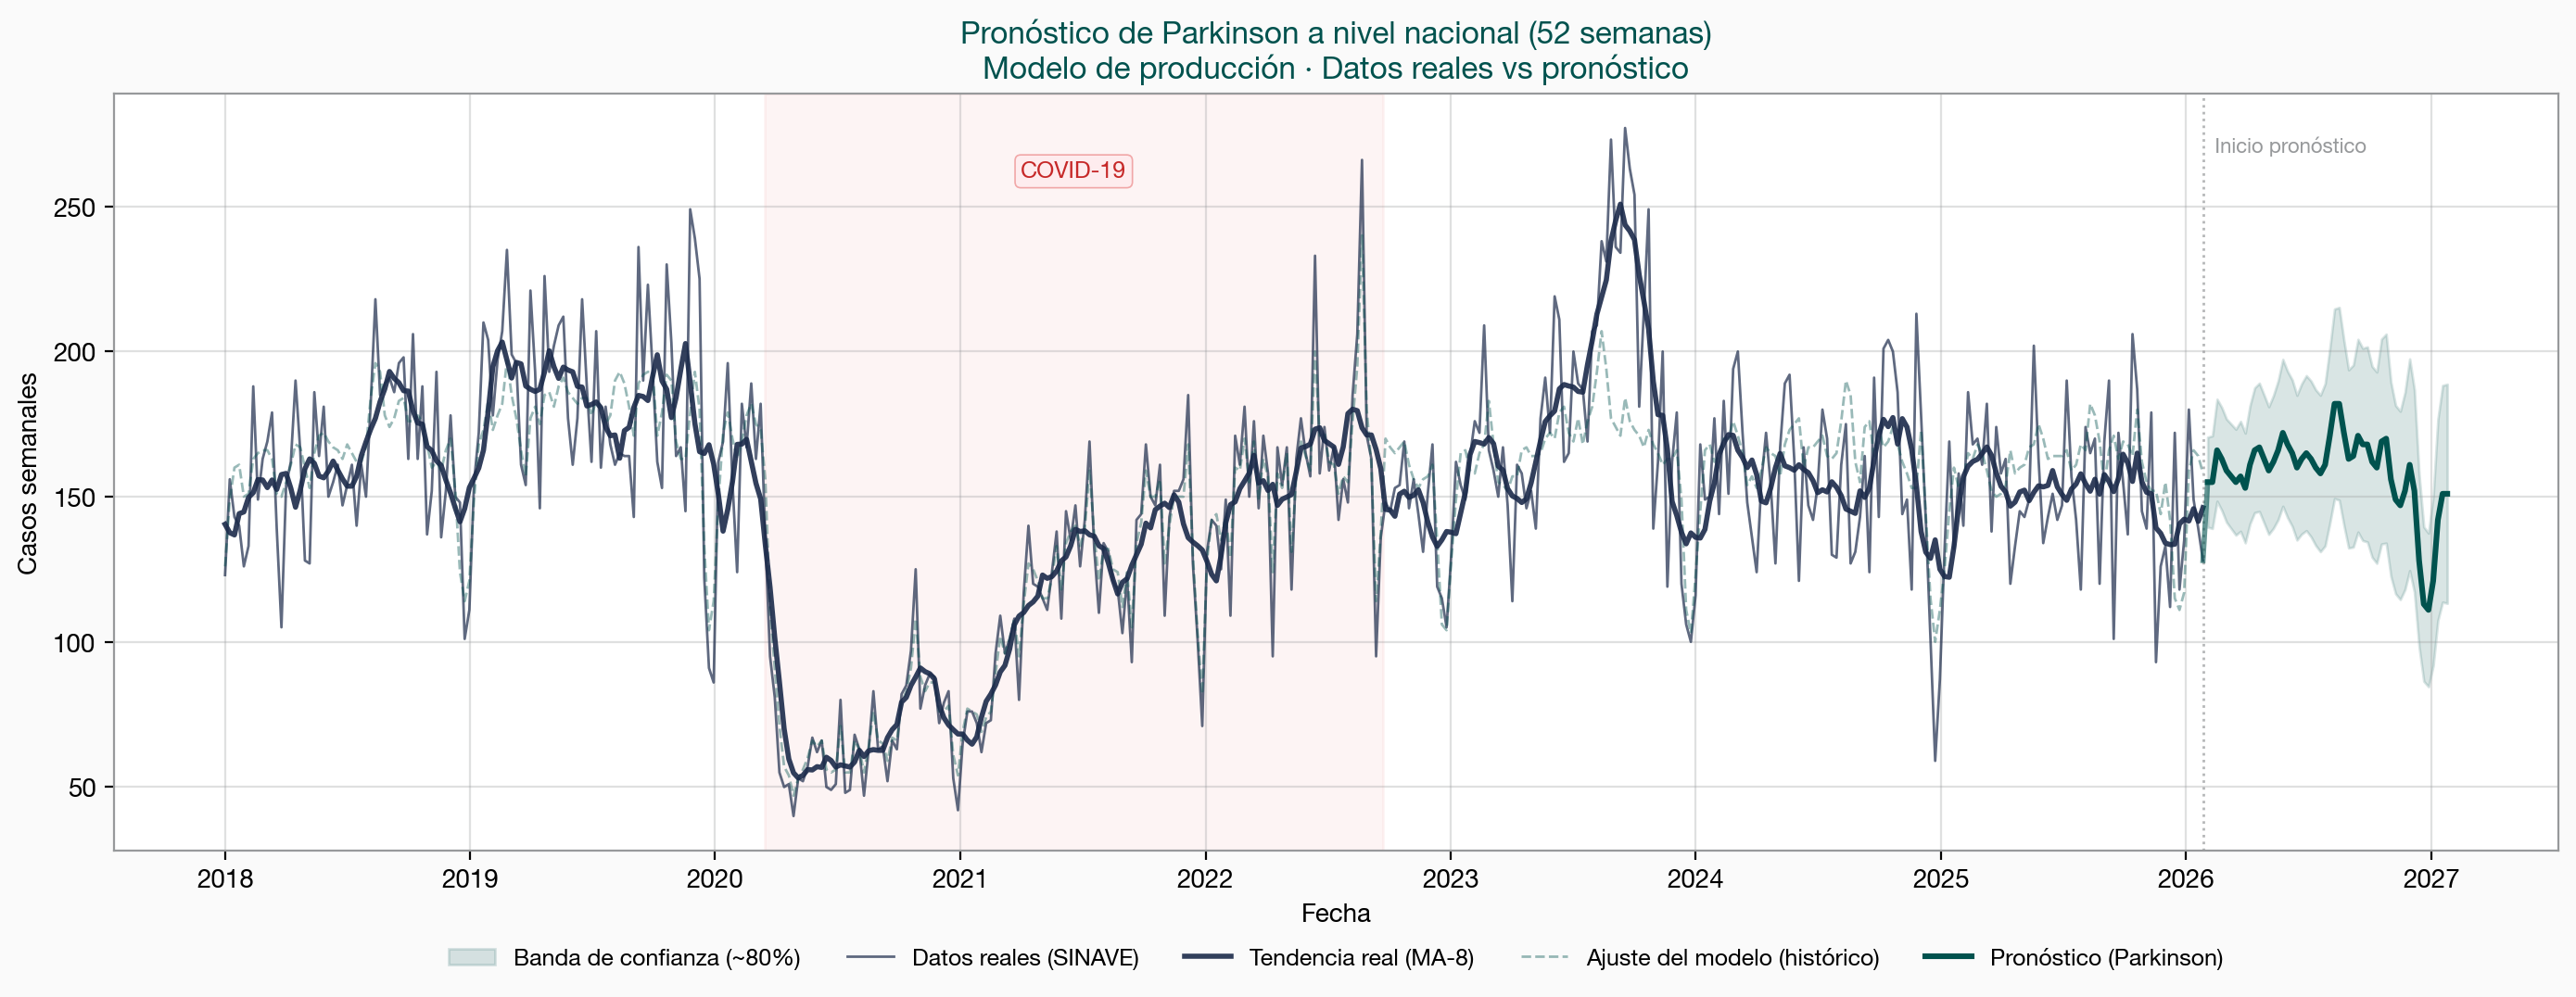
\includegraphics[width=0.95\textwidth]{fig_forecast_parkinson_nacional.png}
  \caption[Pronóstico de Parkinson Nacional.]{Serie real (azul oscuro) vs pronóstico a 52 semanas (verde teal) con banda de confianza al $\sim$80\%, correspondiente a la serie nacional para la cual el motor seleccionado en producción fue Ensemble. La línea punteada muestra el ajuste histórico. Franja roja: periodo COVID-19 (marzo 2020 -- septiembre 2022).}
\label{fig:forecast_parkinson}
\end{figure}

\subsubsection{Mejores y peores estados}

\begin{itemize}[noitemsep]
    \item \textbf{Mejores}: Sinaloa, Veracruz, Guanajuato y Chiapas, con series estables y suficiente volumen de consultas neurológicas.
    \item \textbf{Peores}: Zacatecas, Tlaxcala, Querétaro, Baja California Sur y Nayarit, con baja incidencia observada y alta variabilidad relativa.
\end{itemize}

\subsubsection{Implicaciones clínicas}

\begin{enumerate}[noitemsep]
    \item \textbf{Subdiagnóstico}: la baja incidencia en estados del sur podría reflejar limitaciones en el acceso a neurólogos o subregistro, más que una ausencia real de la enfermedad; esta hipótesis requiere validación clínica adicional.
    \item \textbf{Medicamentos especializados}: levodopa y agonistas dopaminérgicos requieren planificación regional anticipada.
    \item \textbf{Envejecimiento}: la tendencia ascendente demanda inversión a mediano plazo en clínicas de movimiento.
\end{enumerate}

\subsection{Alzheimer (G30)}\label{subsec:alzheimer}

\subsubsection{Insights epidemiológicos}

Alzheimer tiene el menor volumen de incidencia con un pronóstico de \textbf{1,249 casos} a nivel nacional (general) en 52 semanas. La baja incidencia genera un reto estadístico inherente: pequeñas variaciones absolutas producen grandes errores porcentuales.

\begin{itemize}[noitemsep]
    \item \textbf{Tendencia}: estable a ligeramente ascendente, con el mismo patrón de envejecimiento que Parkinson (INEGI, 2024).
    \item \textbf{Estacionalidad}: prácticamente nula a nivel estatal; solo detectable en series agregadas (regional/nacional).
    \item \textbf{Fallback regional}: 7 de las 111 series de Alzheimer utilizan el modelo regional porque la incidencia estatal es insuficiente.
\end{itemize}

La \figref{fig:forecast_alzheimer} muestra el pronóstico nacional generado para este padecimiento.

\begin{figure}[H]
\centering
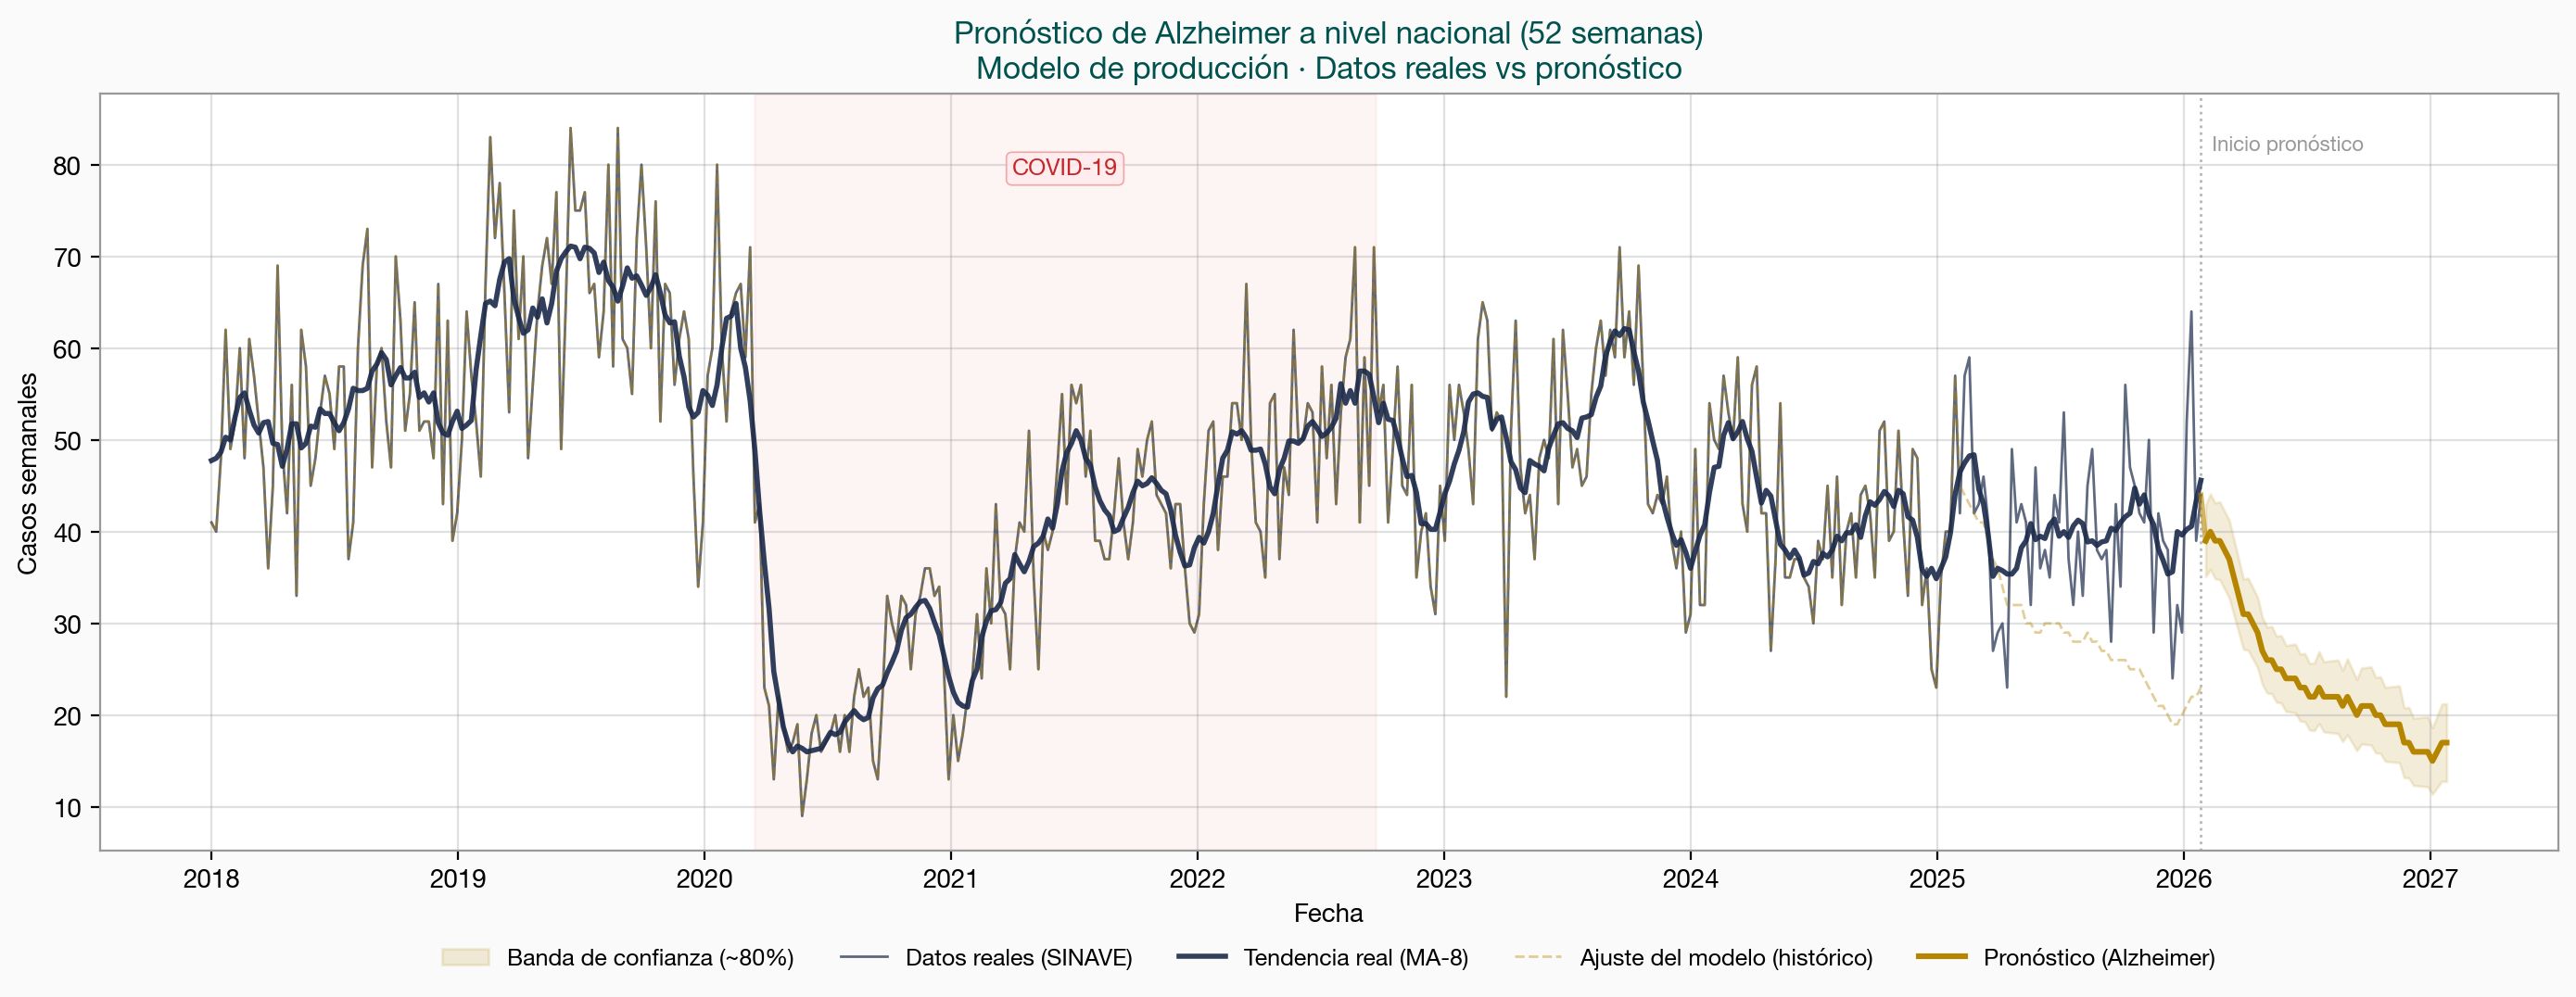
\includegraphics[width=0.95\textwidth]{fig_forecast_alzheimer_nacional.png}

  \caption[Pronóstico de Alzheimer Nacional.]{Serie real (azul oscuro) vs pronóstico del modelo de producción (DeepAR) a 52 semanas (dorado) con banda
  de confianza al $\sim$80\%. La línea punteada muestra el ajuste histórico del modelo. Franja roja: periodo COVID-19 (marzo 2020 -- septiembre 2022).}
\label{fig:forecast_alzheimer}
\end{figure}

\subsubsection{El reto de la baja incidencia}

\begin{criticalbox}[Limitación inherente de los modelos]
Cuando una serie tiene 0 a 3 casos por semana, \textbf{cualquier modelo} producirá un \smape{} alto. Esto no es un defecto del algoritmo sino una propiedad matemática: la división por valores cercanos a cero amplifica el error porcentual (Hyndman \& Koehler, 2006). Las métricas absolutas (\rmse{} = 1.0, \mae{} = 0.7) confirman que los modelos están a menos de 1 caso de la realidad en promedio, lo cual es clínicamente útil.
\end{criticalbox}

\subsubsection{Implicaciones clínicas}

\begin{enumerate}[noitemsep]
    \item \textbf{Posible subregistro}: la diferencia entre la carga esperada de enfermedad en población envejecida (INEGI, 2024) y los casos registrados en SINAVE podría ser consistente con subregistro o con limitaciones de captación del sistema; esta hipótesis requiere validación epidemiológica adicional.
    \item \textbf{Cuidadores}: los pronósticos pueden orientar la planificación de programas de apoyo a cuidadores primarios.
    \item \textbf{Investigación}: los estados con incidencia reportada cero deben ser priorizados para estudios epidemiológicos de campo.
\end{enumerate}

\newpage
% =============================================================================
% 8. ANALISIS DE PROVEEDORES CLOUD
% =============================================================================
\section{Análisis de Proveedores Cloud}\label{sec:cloud}

\subsection{Metodología de evaluación}

Se evaluaron cuatro proveedores de servicios cloud para el despliegue productivo de EpiForecast-MX, utilizando una metodología de puntuación ponderada con 8 factores. La evaluación integra tanto las especificaciones oficiales de cada plataforma (AWS, 2025; Google Cloud, 2025; Microsoft Azure, 2025; IBM, 2025) como la experiencia directa del equipo con AWS SageMaker. Cada factor se pondera según su relevancia para un sistema de pronóstico epidemiológico institucional:

\begin{table}[H]
\centering
\caption{Factores de evaluación y ponderación}
\label{tab:factores_cloud}
\small
\begin{tabularx}{\textwidth}{l c X}
\toprule
\textbf{Factor} & \textbf{Peso} & \textbf{Justificación} \\
\midrule
Costo por entrenamiento     & 20\% & Presupuesto institucional limitado \\
Integración con PyTorch     & 15\% & DeepAR requiere PyTorch nativo \\
AutoML / managed training   & 15\% & Reducir carga operativa del equipo \\
Escalabilidad (GPU)         & 12\% & Crecimiento a más padecimientos \\
Ecosistema de datos         & 12\% & Almacenamiento, ETL, monitoreo \\
Soporte en México           & 10\% & Localidad de datos (LFPDPPP) \\
Documentación / comunidad   & 8\%  & Velocidad de resolución de problemas \\
Seguridad y compliance      & 8\%  & Requisitos institucionales IMSS \\
\bottomrule
\end{tabularx}
\end{table}

\subsection{Tabla comparativa}

\begin{table}[H]
\centering
\caption{Comparativa de proveedores cloud para EpiForecast-MX}
\label{tab:comparativa_cloud}
\scriptsize
\setlength{\tabcolsep}{3pt}
\begin{tabularx}{\textwidth}{X cccc}
\toprule
\textbf{Factor (Peso)} & \textbf{AWS SageMaker} & \textbf{Google Vertex AI} & \textbf{Azure ML} & \textbf{IBM watsonx.ai} \\
\midrule
Costo por entrenamiento (20\%) & \cellcolor{lightgreen}9 & 8 & 7 & 6 \\
Integración PyTorch (15\%) & \cellcolor{lightgreen}10 & 9 & 8 & 7 \\
AutoML / managed (15\%) & \cellcolor{lightgreen}9 & \cellcolor{lightgreen}9 & 8 & 7 \\
Escalabilidad GPU (12\%) & \cellcolor{lightgreen}10 & 9 & 9 & 7 \\
Ecosistema datos (12\%) & \cellcolor{lightgreen}10 & 9 & 8 & 7 \\
Soporte México (10\%) & 8 & 8 & \cellcolor{lightgreen}9 & 7 \\
Documentación (8\%) & \cellcolor{lightgreen}9 & \cellcolor{lightgreen}9 & 8 & 7 \\
Seguridad (8\%) & 9 & 9 & \cellcolor{lightgreen}10 & 8 \\
\midrule
\textbf{Puntuación ponderada} & \cellcolor{lightgreen}\textbf{9.3} & \textbf{8.7} & \textbf{8.2} & \textbf{6.9} \\
\bottomrule
\end{tabularx}
{\scriptsize Nota: puntuaciones calculadas como promedio ponderado (escala 1--10) con los pesos indicados; redondeadas a un decimal.}
\end{table}

La comparativa visual de estas puntuaciones se presenta en el \figref{fig:radar_cloud}, destacando la superioridad técnica y económica de AWS para este proyecto.

\begin{figure}[H]
\centering
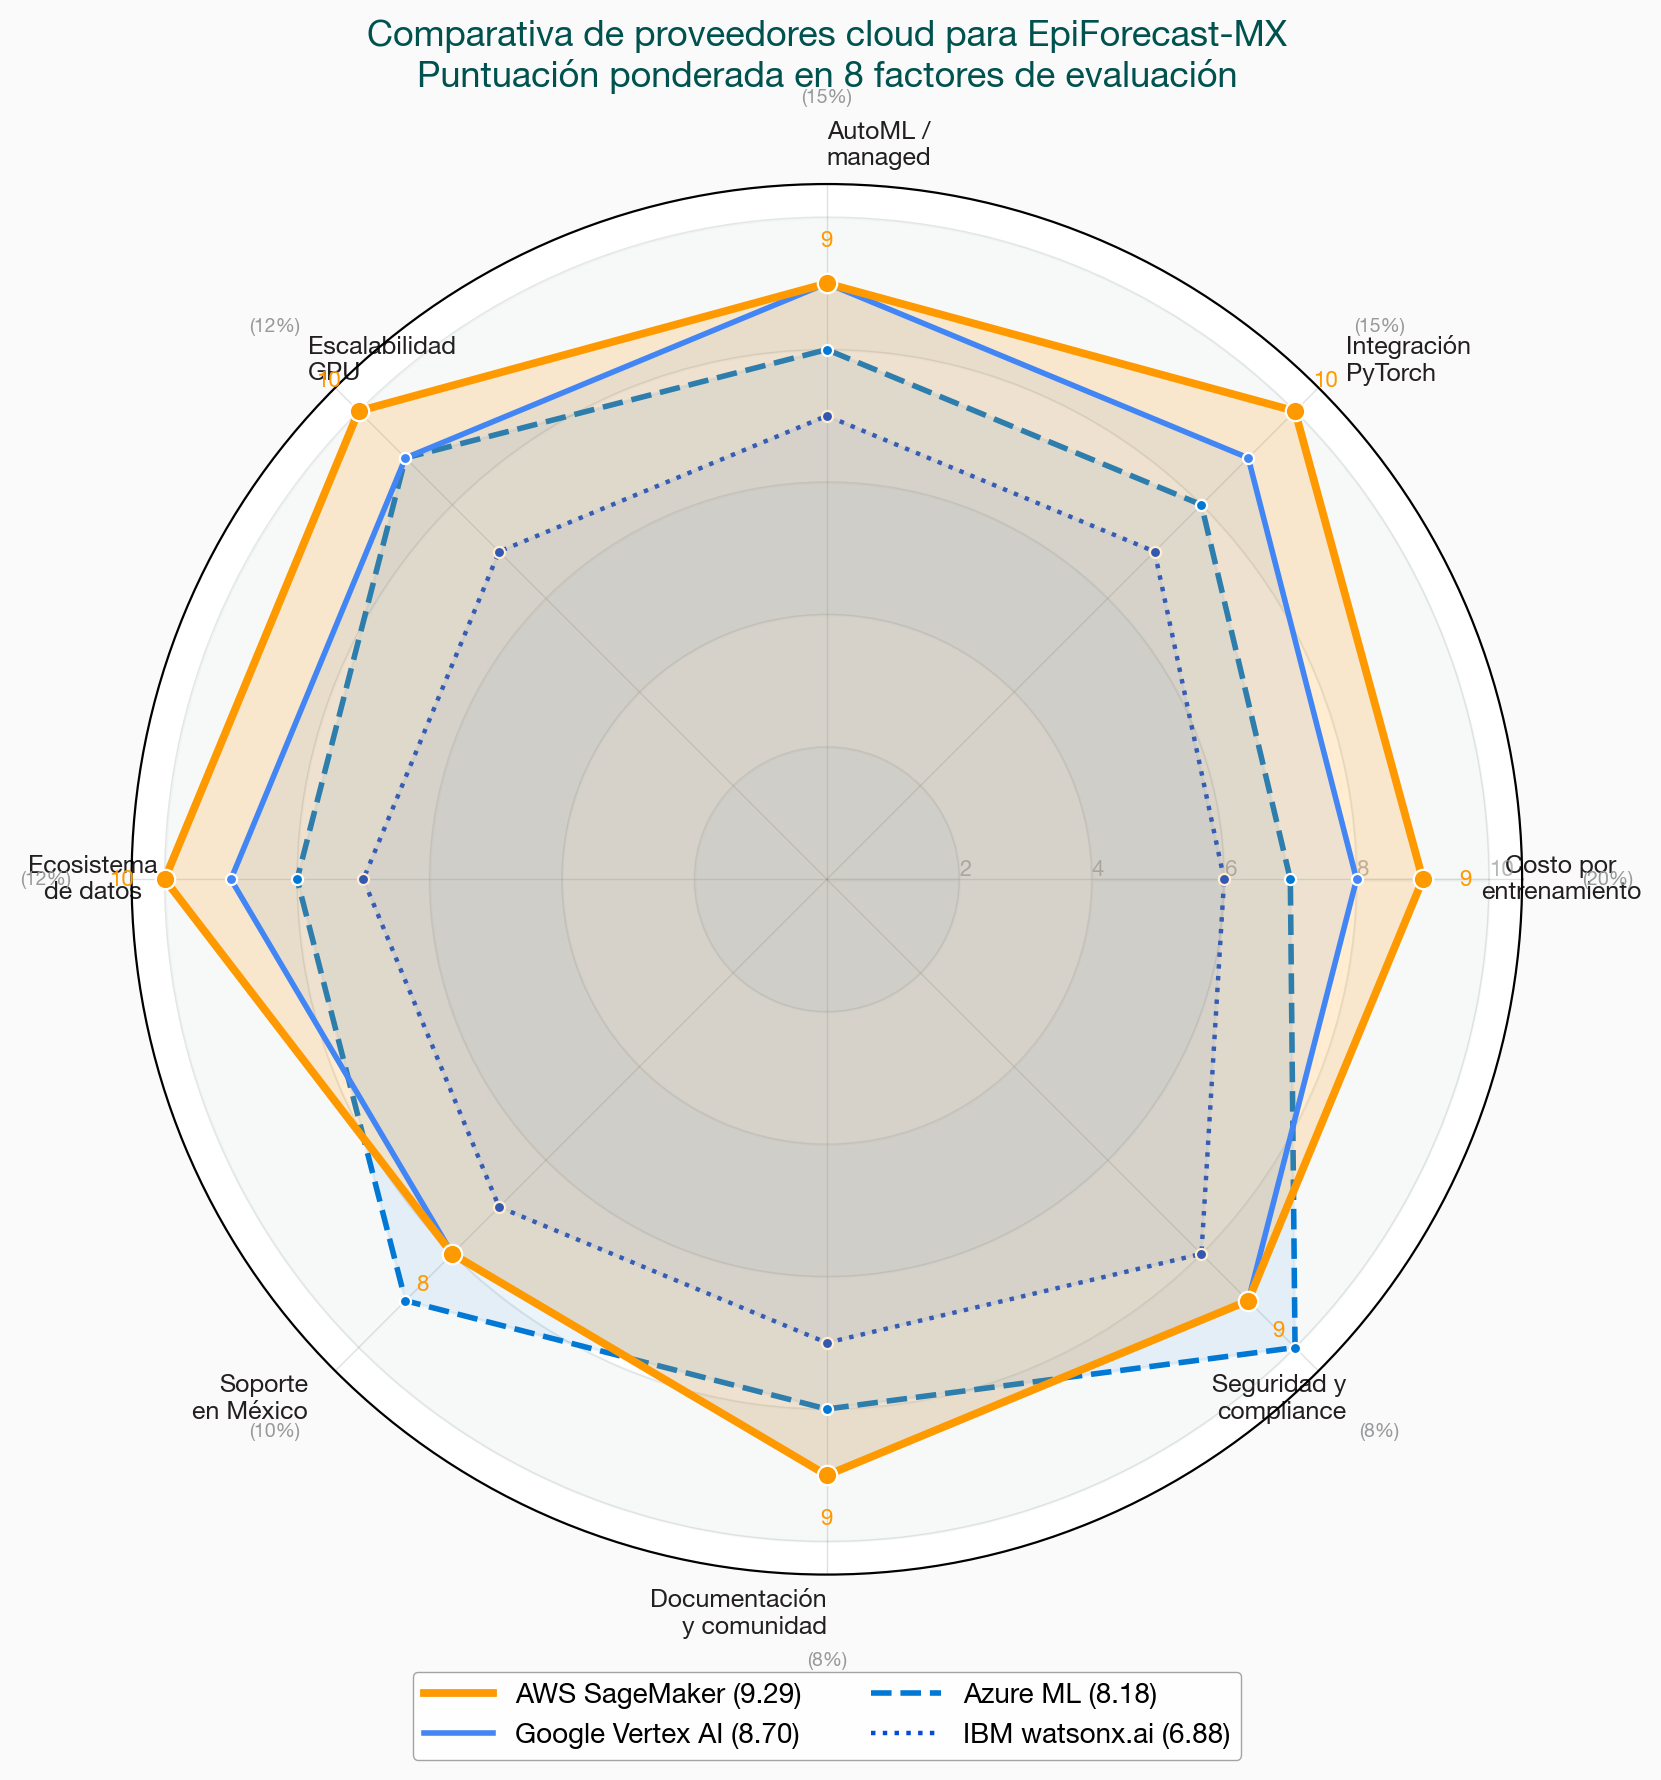
\includegraphics[width=0.75\textwidth]{fig_radar_cloud_providers.png}
\caption[Radar comparativo de nubes.]{Puntuación de los cuatro proveedores en los 8 factores de evaluación; AWS SageMaker presenta el polígono de mayor área.}
\label{fig:radar_cloud}
\end{figure}

\subsection{AWS SageMaker (recomendación primaria)}

AWS SageMaker es la plataforma recomendada con base en la experiencia directa del proyecto (AWS, 2025):

\begin{itemize}[noitemsep]
    \item \textbf{Experiencia real}: se entrenó DeepAR en instancias \texttt{ml.g4dn.xlarge} (NVIDIA T4, 16 GB VRAM) con un costo de \textbf{\$3.50\,--\,\$8.50 USD} por job de entrenamiento completo (333 modelos, 3 padecimientos), como se evidencia en la \figref{fig:sagemaker_training}.
    \item \textbf{Contenerización}: imagen Docker basada en {\small\texttt{pytorch/\allowbreak pytorch:\allowbreak 2.5.1-\allowbreak cuda12.4-\allowbreak cudnn9-\allowbreak runtime}}, construida (\figref{fig:docker_build}) y desplegada automáticamente a ECR (\figref{fig:ecr_repo}).
    \item \textbf{Integración nativa}: S3 para datos, ECR para imágenes, CloudWatch para logs y métricas de rendimiento (\figref{fig:gpu_metrics}).
    \item \textbf{Escalabilidad}: soporte para entrenamiento distribuido y multi-GPU sin cambios de código.
\end{itemize}

\begin{figure}[H]
\centering
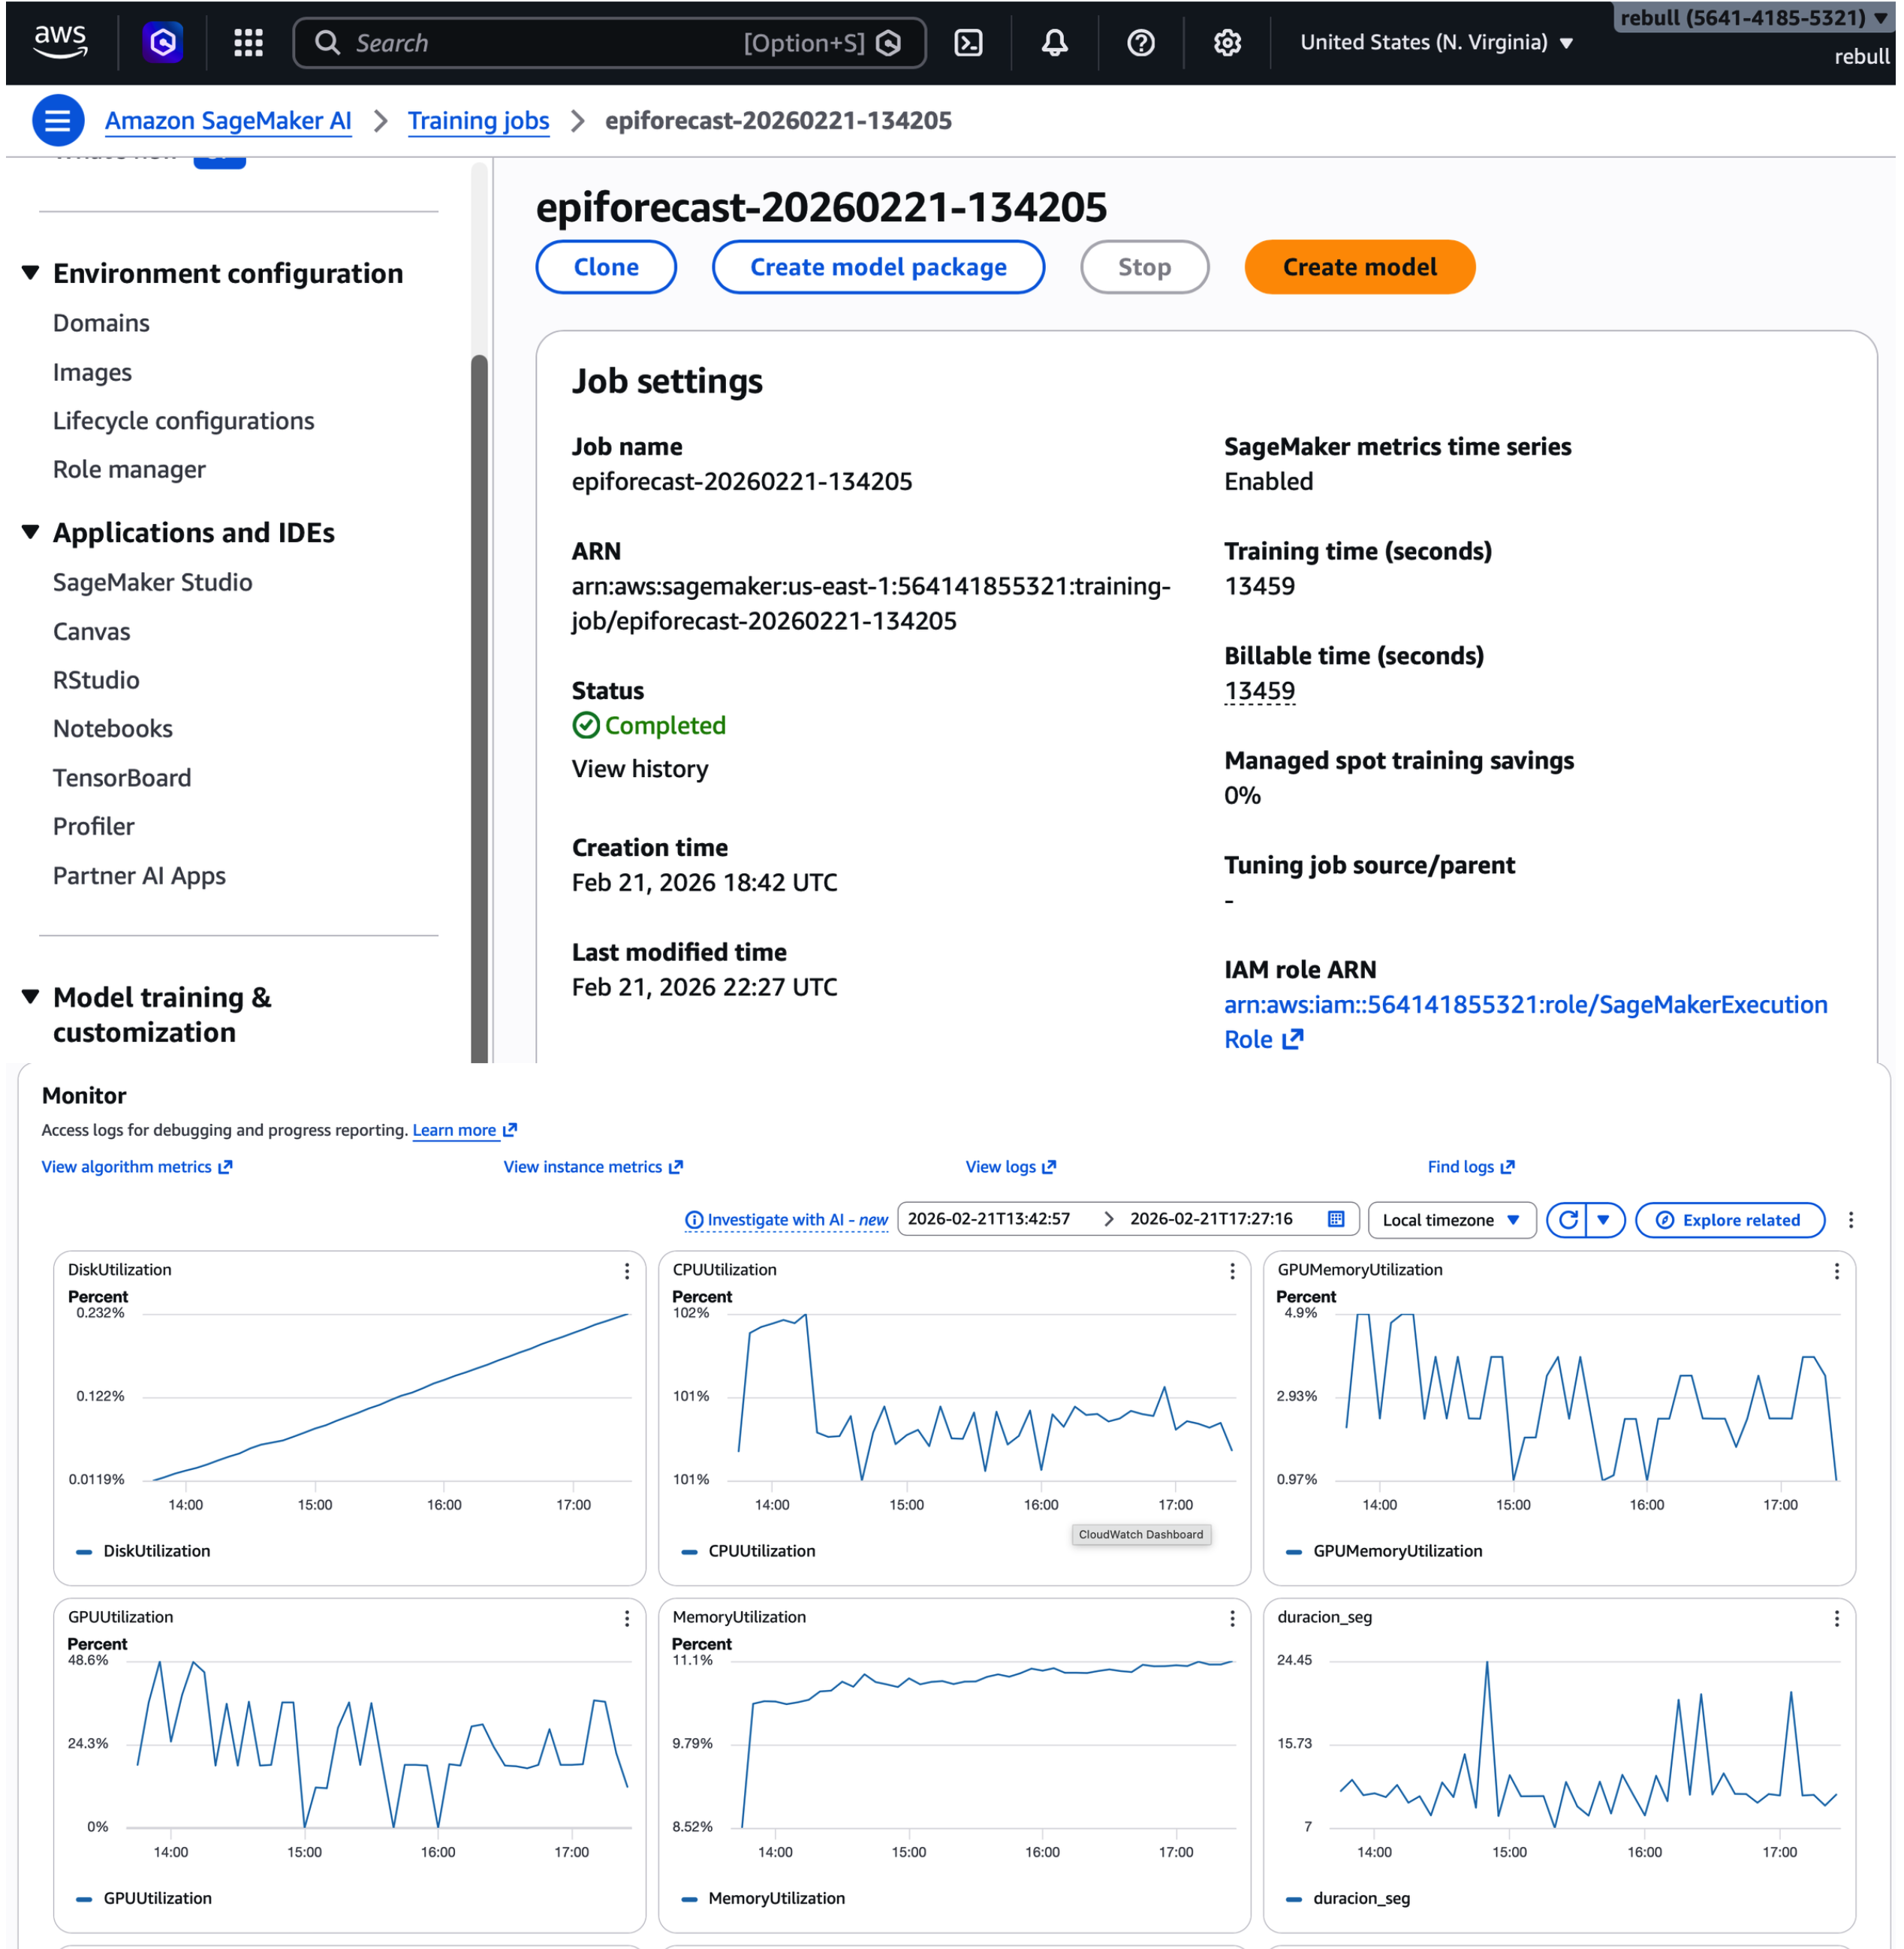
\includegraphics[width=0.95\textwidth]{fig_sagemaker_training.png}
\caption[Training Job en SageMaker.]{Consola de AWS SageMaker mostrando un training job de DeepAR completado exitosamente.}
\label{fig:sagemaker_training}
\end{figure}

\begin{figure}[H]
\centering
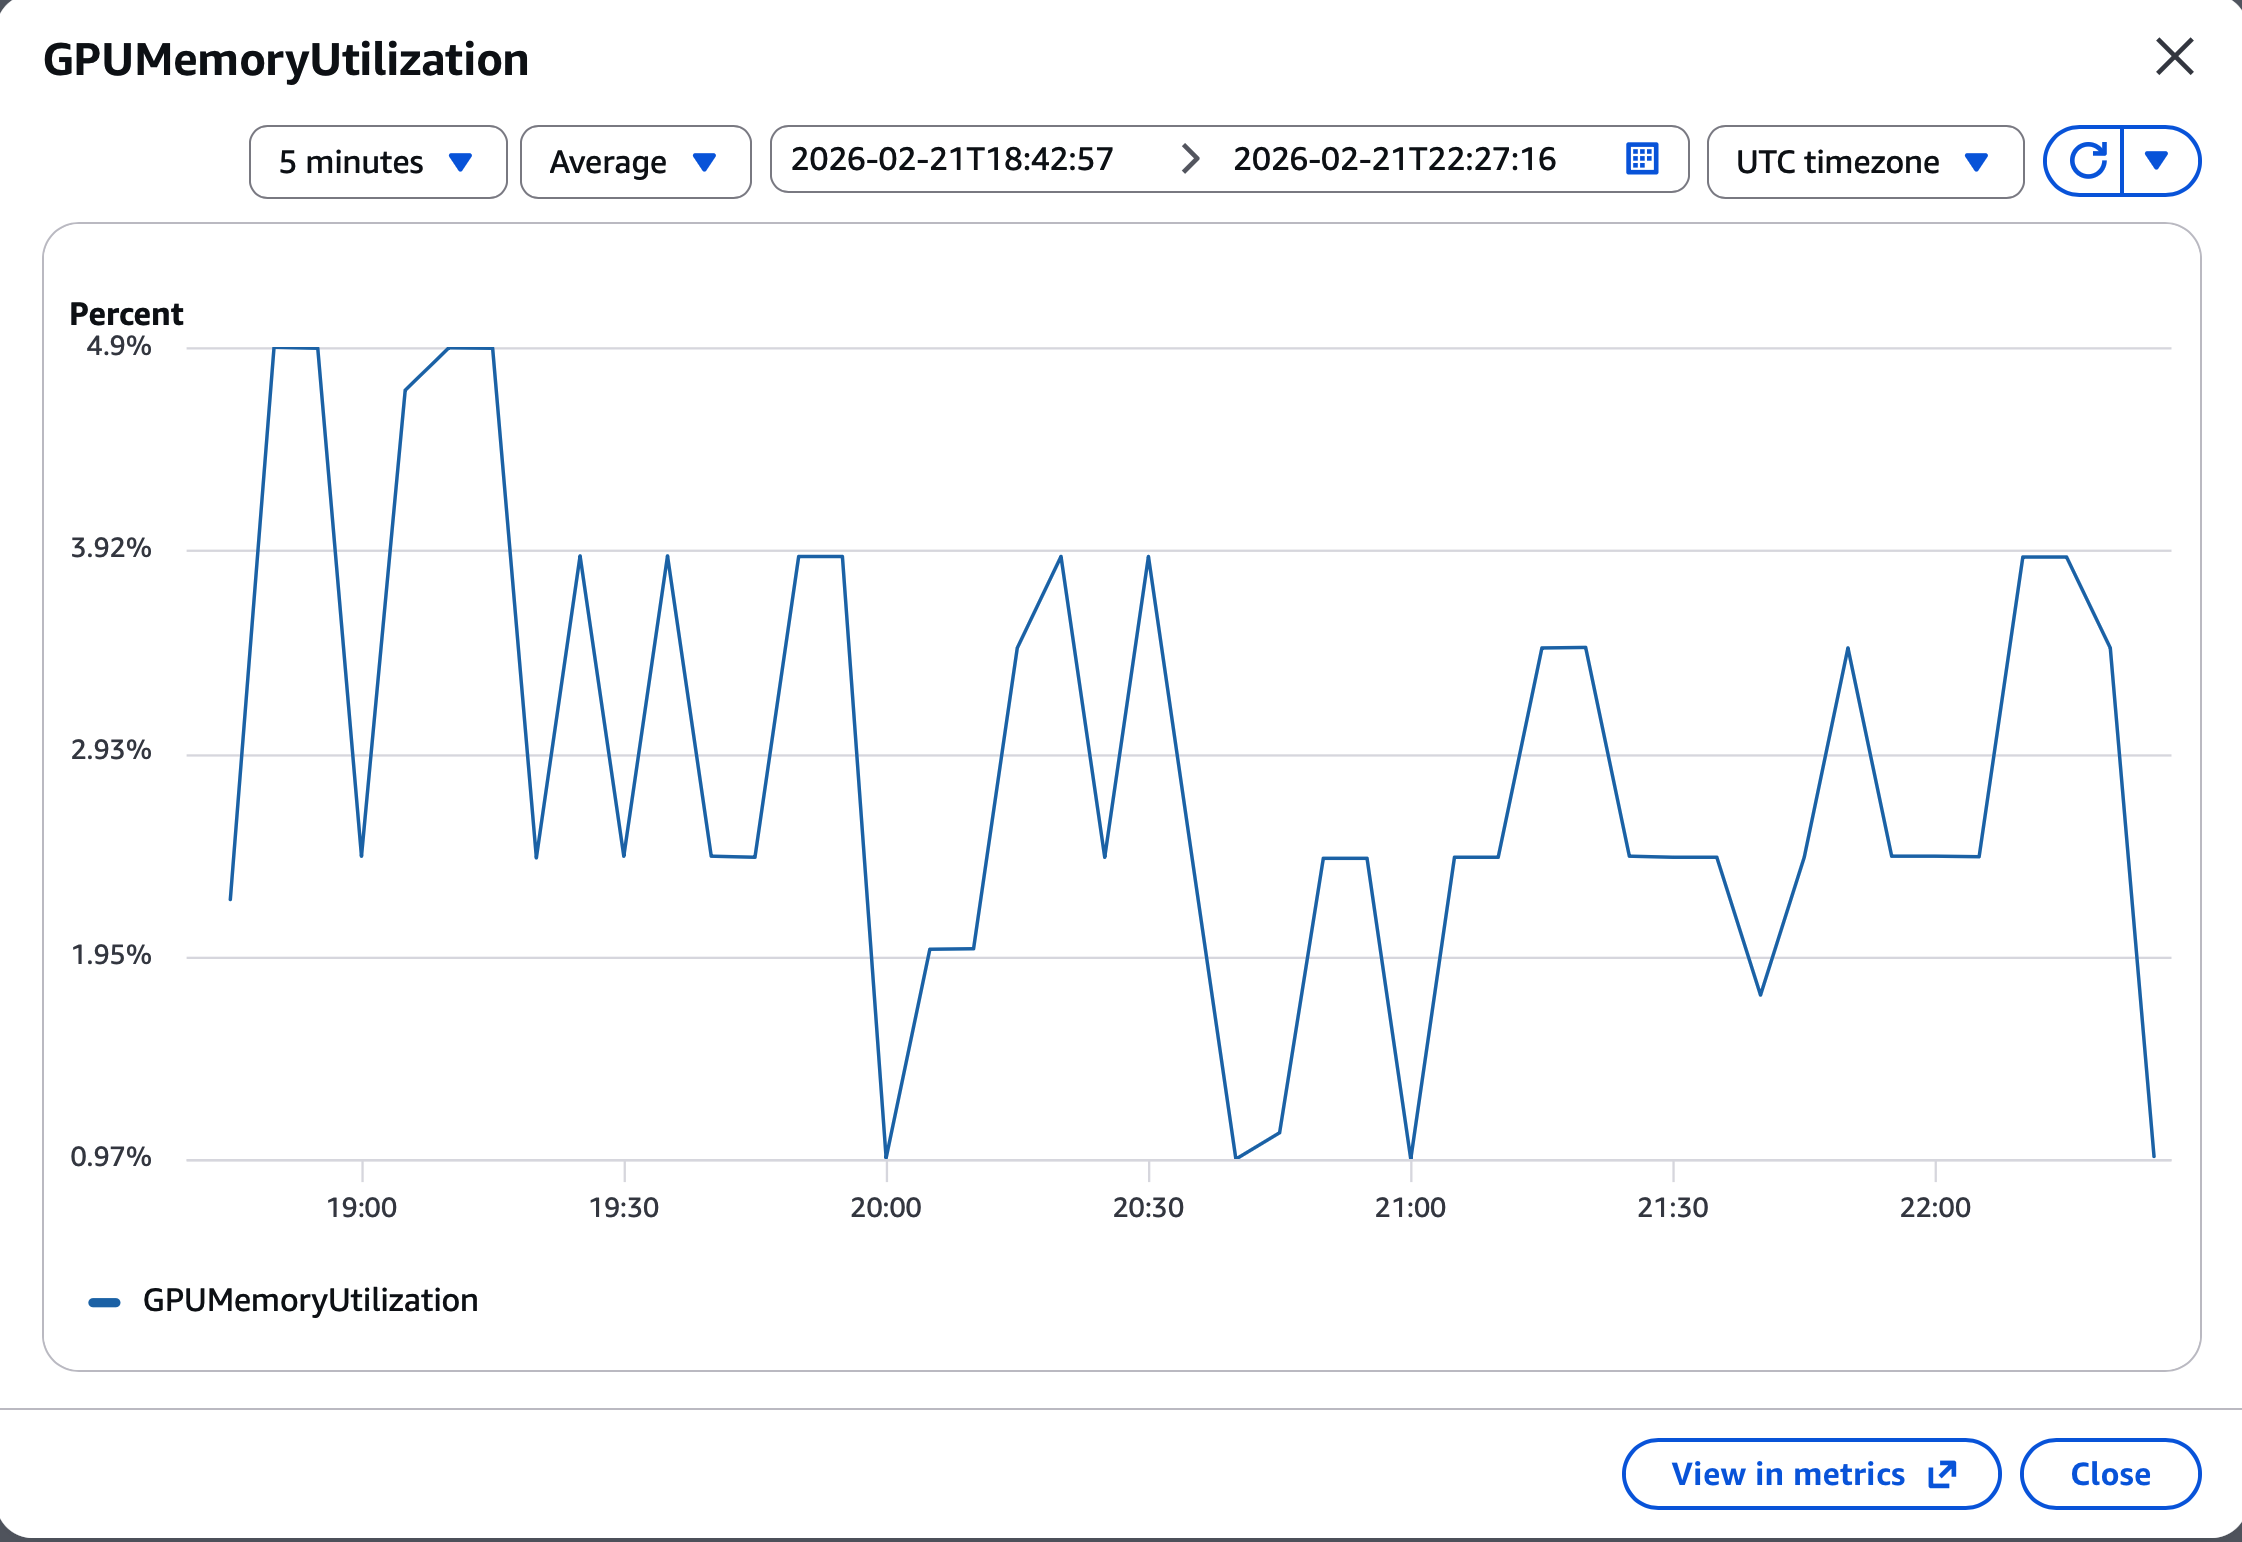
\includegraphics[width=0.95\textwidth]{fig_sagemaker_gpu_metrics.png}
\caption[Métricas GPU en CloudWatch.]{Monitoreo de utilización de GPU (65--85\%) y memoria durante el entrenamiento en SageMaker.}
\label{fig:gpu_metrics}
\end{figure}

\begin{figure}[H]
\centering
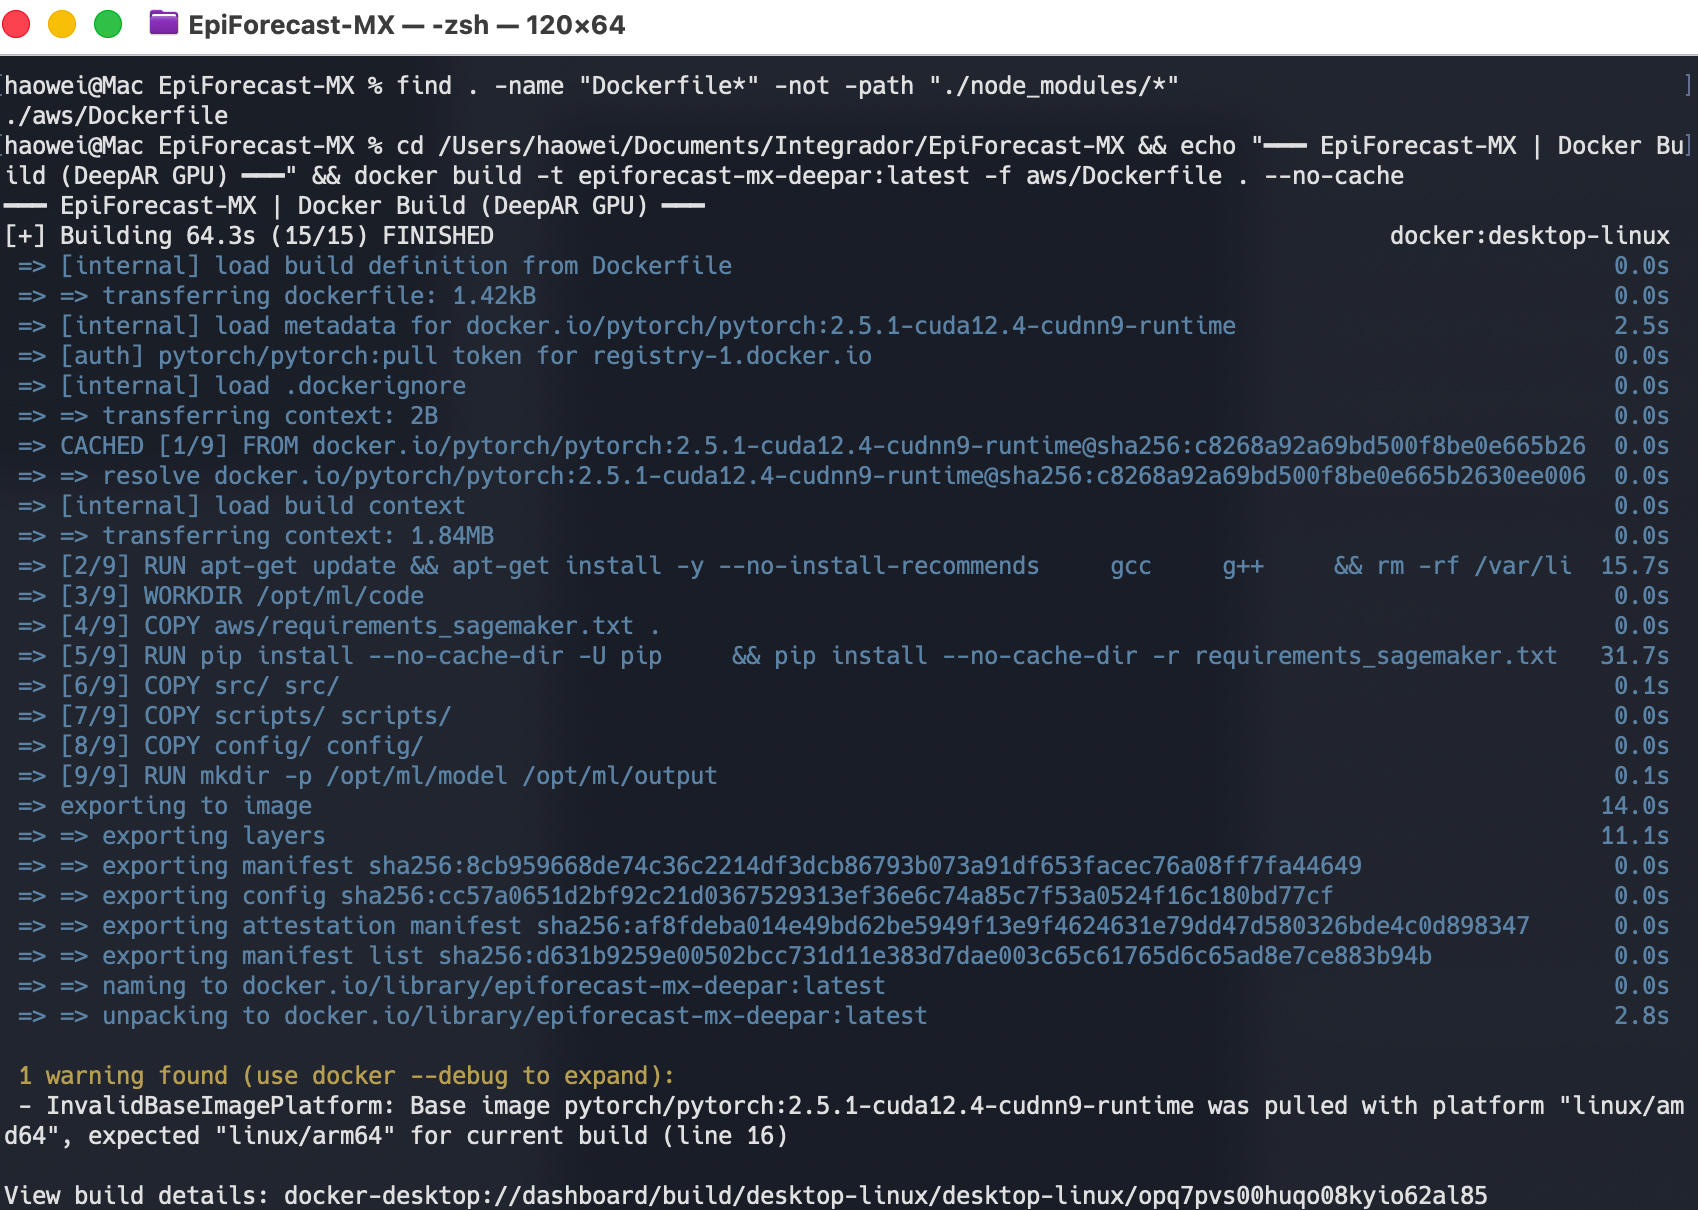
\includegraphics[width=0.90\textwidth]{fig_docker_build.png}
\caption[Build de imagen Docker.]{Proceso de construcción de la imagen Docker optimizada para DeepAR.}
\label{fig:docker_build}
\end{figure}

\begin{figure}[H]
\centering
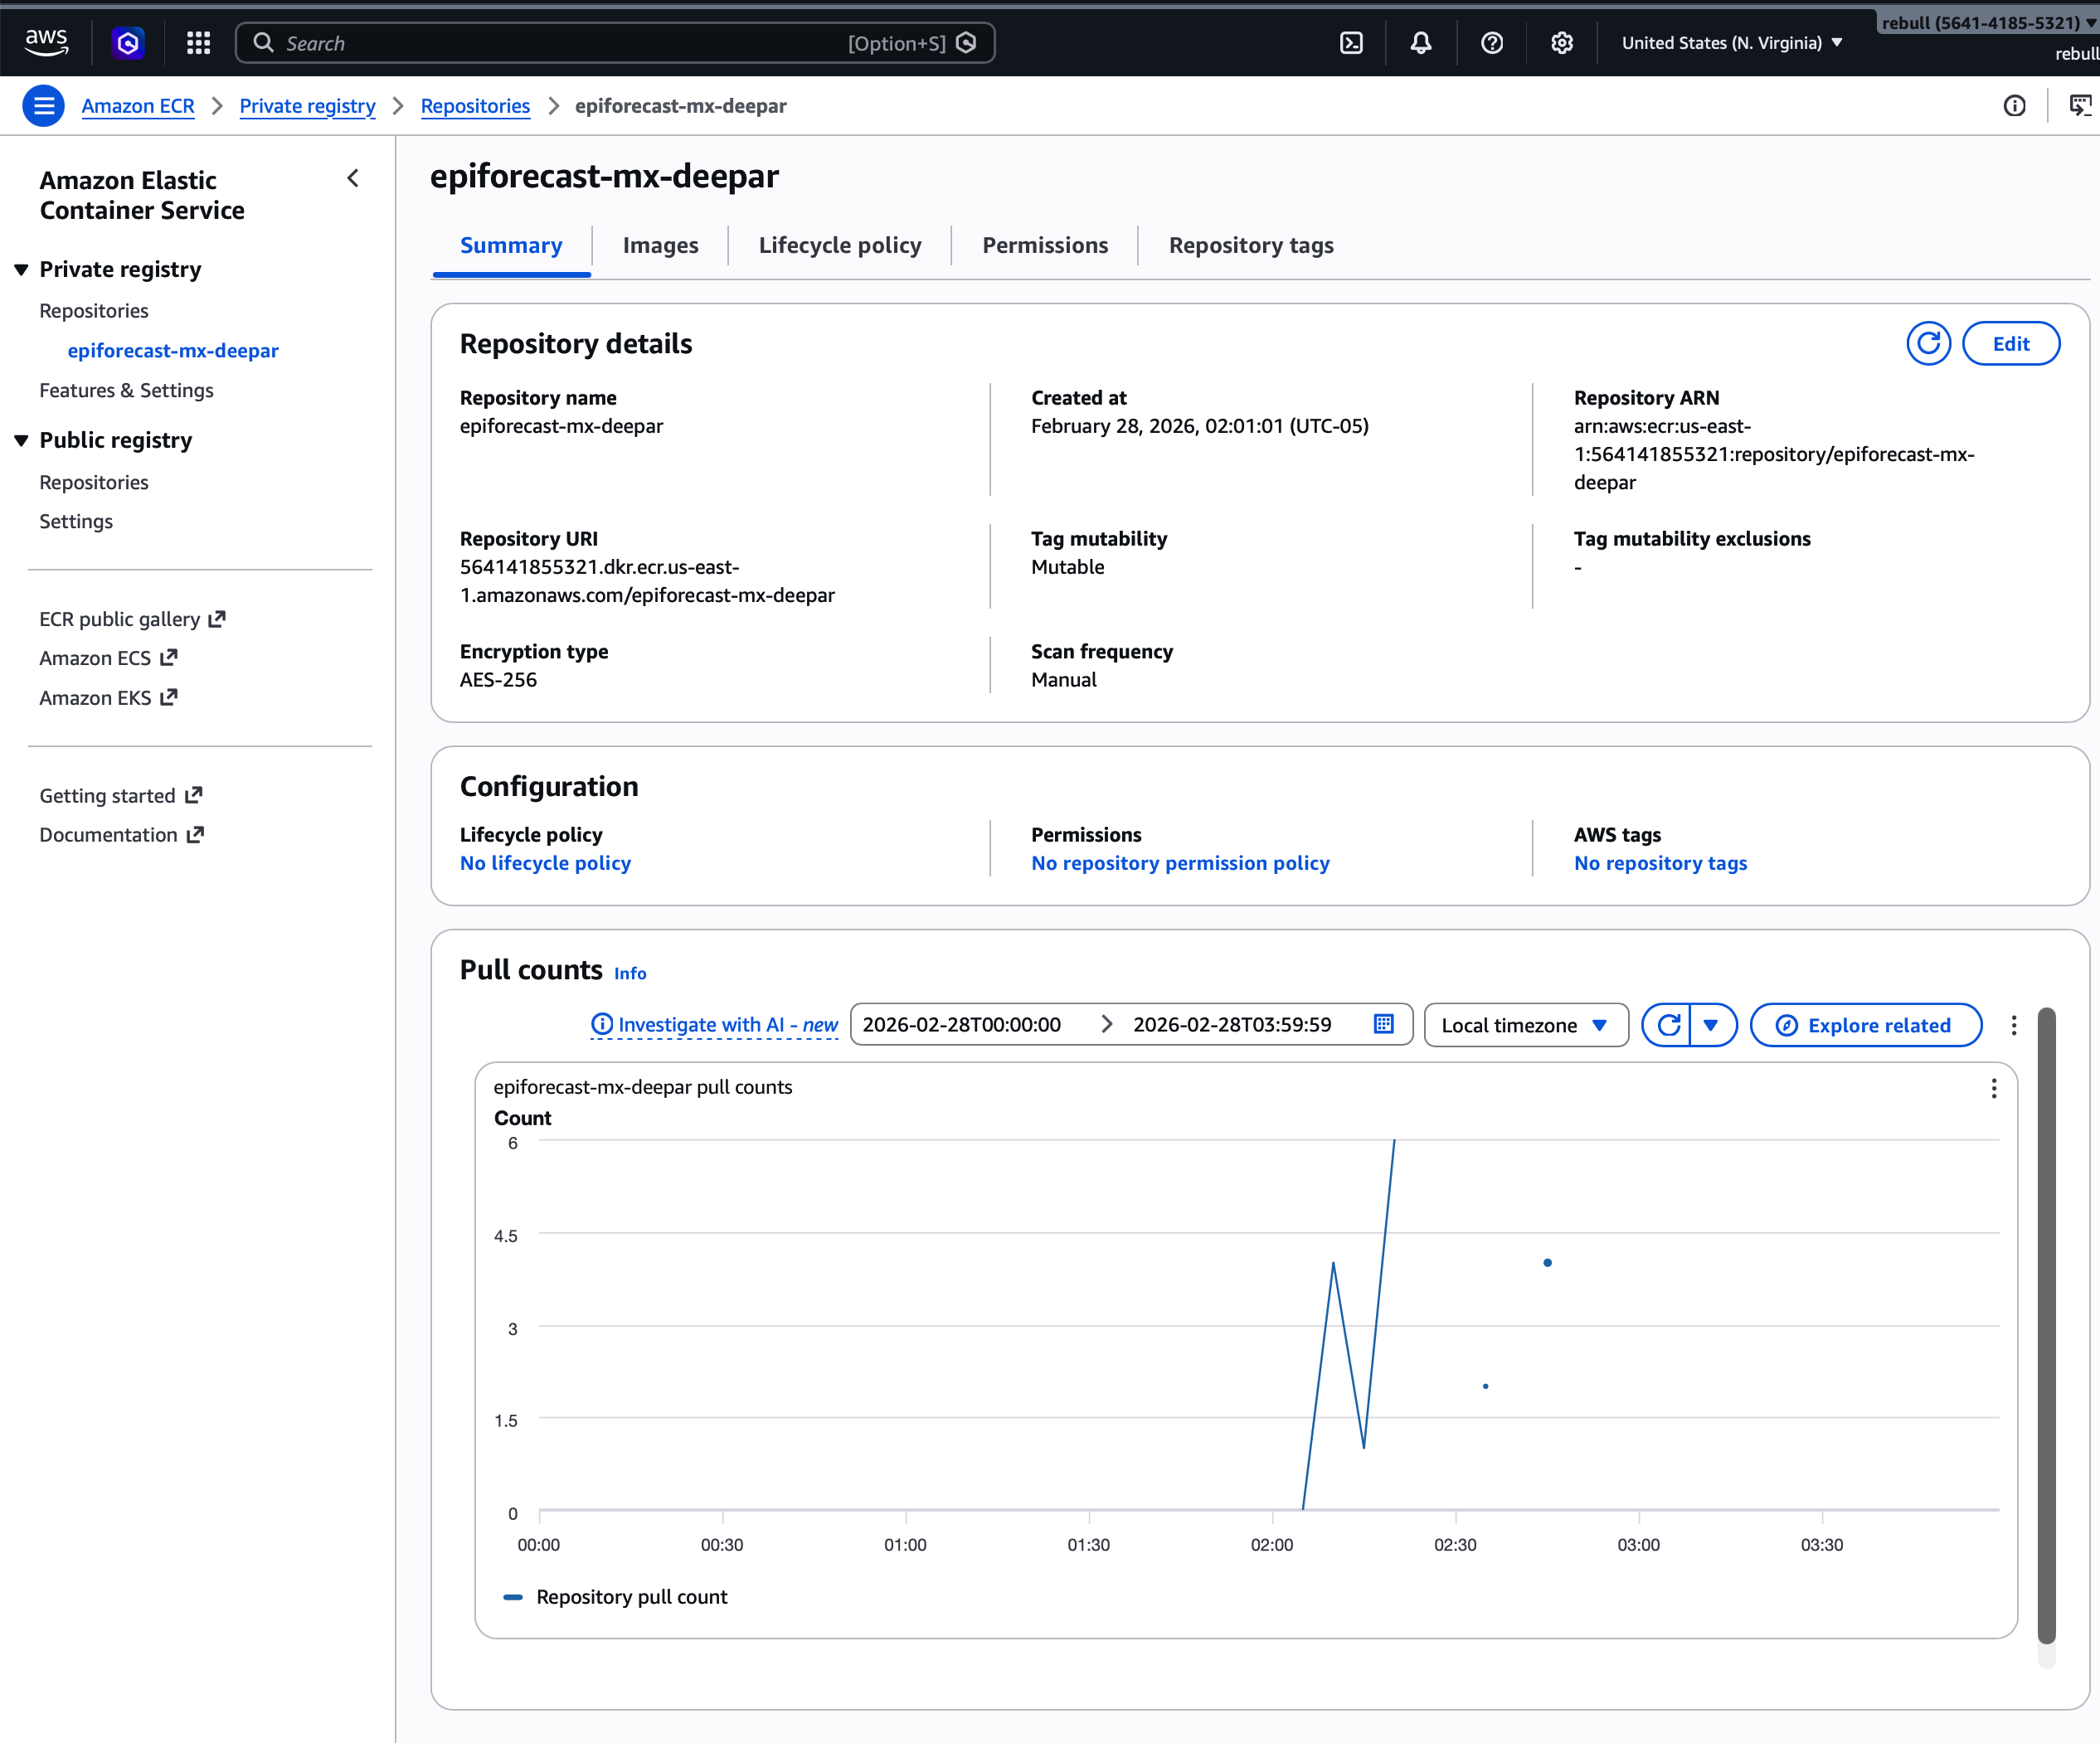
\includegraphics[width=0.90\textwidth]{fig_ecr_repository.png}
\caption[Repositorio Amazon ECR.]{Repositorio ECR con la imagen Docker de EpiForecast-MX publicada y versionada.}
\label{fig:ecr_repo}
\end{figure}

\begin{table}[H]
\centering
\caption{Costos reales de entrenamiento en AWS SageMaker}
\label{tab:costos_sagemaker}
\scriptsize
\begin{tabularx}{\textwidth}{X r r l}
\toprule
\textbf{Componente} & \textbf{\shortstack[r]{Costo unitario\\(USD)}} & \textbf{\shortstack[r]{Costo operativo\\total (USD)}} & \textbf{Nota} \\
\midrule
ml.g4dn.xlarge (GPU) & \$0.736/hr & \$3.50\,--\,8.50 & Rango observado en logs \\
S3 (almacenamiento)  & \$0.023/GB & $\approx$\$0.50 & Datos + modelos \\
ECR (imágenes)       & \$0.10/GB  & $\approx$\$0.30 & Imagen Docker \\
CloudWatch (logs)    & \$0.50/GB  & $\approx$\$0.10 & Logs entrenamiento \\
\midrule
\textbf{Total por job de entrenamiento} & & \multicolumn{2}{r}{\textbf{\$4.40\,--\,9.40 USD}} \\
\bottomrule
\end{tabularx}
\end{table}

\subsection{Google Cloud Vertex AI (alternativa secundaria)}

Google Cloud Vertex AI ofrece una alternativa competitiva (Google Cloud, 2025):

\begin{itemize}[noitemsep]
    \item \textbf{AutoML}: capacidades nativas de AutoML para series de tiempo (Temporal Fusion Transformer).
    \item \textbf{Vertex Pipelines}: orquestación de pipelines ML similar a SageMaker Pipelines.
    \item \textbf{BigQuery ML}: posibilidad de entrenar modelos directamente desde SQL.
    \item \textbf{Costo}: ligeramente superior a AWS para GPU on-demand, pero competitivo con preemptible instances.
\end{itemize}

\subsection{Azure Machine Learning}

Azure ML destaca en seguridad y compliance (Microsoft Azure, 2025):

\begin{itemize}[noitemsep]
    \item \textbf{Región México}: centro de datos en Querétaro para cumplimiento de la LFPDPPP.
    \item \textbf{Active Directory}: integración nativa con la infraestructura de identidad del {\imss}.
    \item \textbf{Costo}: primas ligeramente superiores, justificadas por el ecosistema de compliance.
\end{itemize}

\subsection{IBM watsonx.ai}

IBM watsonx.ai queda en cuarta posición (IBM, 2025):

\begin{itemize}[noitemsep]
    \item \textbf{Fortaleza}: sólida reputación en el sector salud y experiencia con instituciones gubernamentales.
    \item \textbf{Debilidad}: ecosistema menos maduro para PyTorch puro; orientado a modelos propios.
    \item \textbf{Costo}: estructura de precios menos transparente que AWS/GCP.
\end{itemize}

\begin{insightbox}[Recomendación final]
\textbf{AWS SageMaker} es la opción recomendada por su combinación de experiencia real validada, costo comprobado (\$3.50\,--\,\$8.50 USD por job de entrenamiento), ecosistema maduro y escalabilidad. Como alternativa de contingencia, \textbf{Google Vertex AI} ofrece capacidades comparables. La migración entre proveedores es viable gracias al uso de contenedores Docker estándar.
\end{insightbox}

\newpage
% =============================================================================
% 9. ACCIONABLES POR STAKEHOLDER
% =============================================================================
\section{Accionables por Stakeholder}\label{sec:accionables}

\subsection{Matriz de asignación}

La siguiente matriz define \textbf{quién} debe hacer \textbf{qué} y \textbf{para cuándo}, organizando las acciones por stakeholder del ecosistema EpiForecast-MX. Como señala Korolov (2022), medir y asignar el impacto de los sistemas de IA es fundamental para su adopción institucional.

\begin{table}[H]
\centering
\caption{Matriz de accionables por stakeholder}
\label{tab:accionables}
\scriptsize
\setlength{\tabcolsep}{3pt}
\begin{tabularx}{\textwidth}{>{\bfseries}l X l l}
\toprule
\textbf{Stakeholder} & \textbf{Acción} & \textbf{Plazo} & \textbf{Prioridad} \\
\midrule
\multirow{4}{*}{\shortstack[l]{IMSS\\Clínico}} & Integrar pronósticos en planificación mensual de insumos & 3 meses & Alta \\
& Definir umbrales de alerta por estado (ej.: $>$20\% de incremento) & 2 meses & Alta \\
& Capacitar epidemiólogos delegacionales en lectura del dashboard & 4 meses & Media \\
& Establecer protocolo de validación semanal de pronósticos con boletines SINAVE & 1 mes & Alta \\
\midrule
\multirow{3}{*}{\shortstack[l]{IMSS\\TI}} & Provisionar cuenta AWS con roles IAM para EpiForecast & 2 meses & Alta \\
& Configurar VPN o Direct Connect para acceso seguro a S3 & 3 meses & Alta \\
& Implementar monitoreo de drift con CloudWatch Alarms & 4 meses & Media \\
\midrule
\multirow{3}{*}{\shortstack[l]{Equipo\\Académico}} & Publicar resultados en foro especializado en salud mental & 6 meses & Media \\
& Documentar metodología para publicación en revista indexada & 9 meses & Media \\
& Transferir conocimiento al equipo IMSS TI (2 sesiones) & 2 meses & Alta \\
\midrule
\multirow{3}{*}{\shortstack[l]{Equipo\\Técnico}} & Automatizar pipeline de reentrenamiento trimestral (cron/Airflow) & 3 meses & Alta \\
& Agregar monitoreo de \smape{} por serie con alertas automáticas & 3 meses & Alta \\
& Expandir a padecimientos adicionales (diabetes, hipertensión) & 12 meses & Baja \\
\midrule
\multirow{2}{*}{\shortstack[l]{Secretaría\\de Salud}} & Evaluar adopción del framework para vigilancia epidemiológica federal & 12 meses & Baja \\
& Integrar datos de mortalidad del Subsistema Epidemiológico & 9 meses & Media \\
\bottomrule
\end{tabularx}
\end{table}

\subsection{Detalle por stakeholder}

\subsubsection{IMSS Clínico}

El área clínica del {\imss} es el principal beneficiario del sistema. Las acciones prioritarias son:

\begin{enumerate}[noitemsep]
    \item \textbf{Integración en la cadena de suministro}: los pronósticos de Depresión deben alimentar la solicitud trimestral de antidepresivos a nivel delegacional.
    \item \textbf{Alertas tempranas}: definir reglas de negocio (ej.: si el pronóstico supera 1.2$\times$ el valor histórico, activar alerta al coordinador estatal).
    \item \textbf{Validación continua}: cada lunes, comparar el pronóstico de la semana previa contra el boletín SINAVE recién publicado. Si el error acumulado de 4 semanas supera 15\%, solicitar reentrenamiento anticipado fuera del ciclo trimestral.
\end{enumerate}

\subsubsection{IMSS TI}

El área de tecnologías de información es responsable de la infraestructura:

\begin{enumerate}[noitemsep]
    \item \textbf{Acceso AWS}: crear cuenta dedicada con roles IAM: {\small\texttt{Sage\-Maker\-Execution}}, {\small\texttt{S3\-Read\-Write}} y {\small\texttt{ECR\-Pull}}.
    \item \textbf{Red}: establecer conexión segura entre la red IMSS y AWS (VPN site-to-site o Direct Connect).
    \item \textbf{Monitoreo}: implementar dashboards de CloudWatch para uso de GPU, costos y alertas de fallo.
\end{enumerate}

\subsubsection{Equipo Académico}

El equipo del Tec de Monterrey tiene la responsabilidad de difusión y transferencia:

\begin{enumerate}[noitemsep]
    \item \textbf{Transferencia de conocimiento}: dos sesiones presenciales con el equipo IMSS TI cubriendo arquitectura, despliegue y mantenimiento.
    \item \textbf{Publicación}: someter artículo a foros especializados en salud mental (véase \secref{sec:futuro}).
    \item \textbf{Documentación}: mantener actualizado el repositorio GitHub con guías de operación.
\end{enumerate}

\newpage
% =============================================================================
% SISTEMA DE VISUALIZACION TABLEAU
% =============================================================================
\section{Sistema de Visualización Tableau}\label{sec:tableau}

El archivo \texttt{viz\_epiforecastmx.twb} constituye el libro de trabajo de Tableau que implementa el sistema de visualización del proyecto \textbf{EpiForecast-MX}. Su propósito es integrar en una sola plataforma interactiva tres dimensiones analíticas complementarias (exploración epidemiológica, predicción a 52 semanas y monitoreo del sistema de modelado) que, en conjunto, permiten transformar datos complejos en información accionable para tomadores de decisiones clínicas y administrativas del {\imss}. El dashboard está publicado en Tableau Public y accesible desde \url{https://proyectointegrador.org/epidashboard}, sin requerir instalación de software.

\subsection{Arquitectura del flujo de datos}\label{subsec:flujo_tableau}

La \figref{fig:flujo_tableau} presenta el flujo completo de información del sistema, desde las fuentes de datos primarias hasta las visualizaciones embebidas en el sitio web del proyecto.

\begin{figure}[H]
\centering
\resizebox{0.80\textwidth}{!}{%
\begin{tikzpicture}[
    base/.style={thick, rounded corners=6pt,
      minimum width=5.6cm, minimum height=1.3cm, text width=5.4cm,
      align=center, font=\sffamily\normalsize,
      drop shadow={opacity=0.12, shadow xshift=2pt, shadow yshift=-2pt}},
    source/.style ={base, draw=burgundy, fill=lightred!60},
    script/.style ={base, draw=darkteal, fill=lightgreen},
    store/.style  ={base, draw=imssblue, fill=cream},
    cloud/.style  ={base, draw=gold,     fill=lightyellow},
    output/.style ={base, draw=teal,     fill=teal!10},
    filebadge/.style={font=\sffamily\small\ttfamily\color{slateborder},
      fill=slatelight, draw=slateborder,
      inner sep=4pt, rounded corners=3pt, thick, align=center},
    secretbadge/.style={font=\sffamily\small\color{coolgray},
      fill=white, draw=coolgray, dashed,
      inner sep=6pt, rounded corners=5pt, thick,
      align=left, text width=5.0cm},
    autobadge/.style={font=\sffamily\scriptsize\bfseries\color{burntborder},
      fill=burntlight, draw=burntborder,
      inner sep=4pt, rounded corners=4pt, thick,
      align=center, text width=3.6cm},
    edgelabel/.style={font=\sffamily\small\bfseries\color{coolgray},
      fill=white, inner sep=3pt, rounded corners=4pt},
    arrow/.style={-{Stealth[round, length=9pt, width=7pt]},
      thick, color=coolgray, shorten >=3pt, shorten <=3pt},
    arrowdashed/.style={-{Stealth[round, length=9pt, width=7pt]},
      thick, color=coolgray, dashed, shorten >=3pt, shorten <=3pt},
    looparrow/.style={-{Stealth[round, length=9pt, width=7pt]},
      thick, color=burntborder, shorten >=3pt, shorten <=3pt},
]
\node[source] (sinave) at (0, 0)
    {\textbf{SINAVE / INEGI}\\[1mm]\small Datos epidemiológicos crudos};
\node[source] (modelos) at (-12.0, -4.2)
    {\textbf{Modelos Entrenados}\\[1mm]\small Predicciones y métricas de producción};
\node[filebadge, below=0.25cm of modelos, align=center] (modelosbadge)
    {\texttt{all\_forecast\_*.csv}\\[2pt]\texttt{tabla\_333\_modelos\_produccion.xlsx}};
\node[script] (build) at (0, -4.2)
    {\textbf{build\_tableau.py}\\[1mm]\small Pipeline de datos y normalización};
\node[filebadge, below=1.4cm of build, align=center] (xlsxbadge)
    {\texttt{tableau\_model.xlsx}\\[2pt]
     \texttt{scaffold\ |\ real\ |\ forecast\ |\ metricas\ |\ entidades}};
\node[store] (github) at (0, -10.2)
    {\textbf{GitHub Repo}\\[1mm]\small Código fuente \texttt{+} archivo \texttt{.twb}};
\node[filebadge, below=0.25cm of github] (gitbadge)
    {\texttt{EpiForecast-MX.twb\ \ |\ \ gsheets.yml}};
\node[cloud] (gha) at (0, -14.6)
    {\textbf{GitHub Actions}\\[1mm]\small \texttt{gsheets.yml}, trigger automático};
\node[script] (publish) at (0, -19.0)
    {\textbf{publish\_gsheets.py}\\[1mm]\small Publicación por bloques a Google Sheets};
\node[store] (gsheets) at (0, -23.4)
    {\textbf{Google Sheets}\\[1mm]\small Fuente de datos live, acceso público};
\node[filebadge, below=0.45cm of gsheets] (sheetbadge)
    {\texttt{GSHEETS\_SPREADSHEET\_ID}};
\node[cloud] (tableau) at (0, -28.4)
    {\textbf{Tableau Public}\\[1mm]\small Auto-refresh del extract desde Sheets};
\node[output] (website) at (0, -32.8)
    {\textbf{proyectointegrador.org}\\[1mm]\small Visualizaciones embebidas, live};
\node[secretbadge] (secrets) at (10.5, -14.6)
    {\textcolor{coolgray}{\textbf{GitHub Secrets}}\\[4pt]
     \texttt{GOOGLE\_SERVICE\_}\\\texttt{ACCOUNT\_JSON}\\[3pt]
     \texttt{GSHEETS\_SPREADSHEET\_ID}};
\node[autobadge] (badge_refresh) at (5.8, -25.9)
    {$\circlearrowleft$\ \ refresh automático\\cada $\sim$24 horas};
\node[autobadge] (badge_web) at (5.8, -30.6)
    {$\circlearrowleft$\ \ web se actualiza\\automáticamente};
\begin{pgfonlayer}{background}
\draw[arrow] (sinave.south)
    -- node[edgelabel, right=4pt] {datos crudos} (build.north);
\draw[arrow] (modelos.east)
    -- node[edgelabel, below=4pt] {predicciones + métricas} (build.west);
\draw[arrow] (build.south)
    -- node[edgelabel, right=4pt] {genera} (xlsxbadge.north);
\draw[arrow] (xlsxbadge.south)
    -- node[edgelabel, right=4pt] {versionado en repo} (github.north);
\draw[arrow] (github.south)
    -- node[edgelabel, right=4pt] {push \textbar{} workflow\_dispatch} (gha.north);
\draw[arrowdashed] (secrets.west)
    -- node[edgelabel, above=4pt] {inyecta secretos} (gha.east);
\draw[arrow] (gha.south)
    -- node[edgelabel, right=4pt] {ejecuta script} (publish.north);
\draw[arrow] (publish.south)
    -- node[edgelabel, right=4pt] {publica 5 tabs por bloques} (gsheets.north);
\draw[arrow] (gsheets.south) -- (tableau.north);
\draw[arrow] (tableau.south) -- (website.north);
\draw[looparrow]
    (website.east) -- ++(3.0, 0) -- ++(0, 9.4) -- (gsheets.east);
\end{pgfonlayer}
\end{tikzpicture}
}
\caption[Flujo de información del sistema Tableau.]{%
Flujo de información del sistema: desde las fuentes de datos (\textsc{sinave}/\textsc{inegi}
y modelos entrenados) hasta las visualizaciones embebidas en el sitio web,
pasando por el pipeline de normalización, publicación automatizada a Google
Sheets y el ciclo de actualización continua de Tableau Public ($\sim$24 horas).}
\label{fig:flujo_tableau}
\end{figure}

El flujo puede describirse en tres capas funcionales. La \textbf{capa de datos} comprende la ingesta de boletines \textsc{sinave}, la integración con variables demográficas del \textsc{inegi} y la incorporación de los resultados de los 333 modelos de producción. La \textbf{capa de automatización} gestiona la publicación del dataset mediante GitHub Actions y la sincronización con Google Sheets como fuente de datos live para Tableau Public. La \textbf{capa de presentación} expone los dashboards embebidos en el sitio web del proyecto, actualizándose automáticamente cada $\sim$24 horas sin intervención manual.

\newpage
\subsection{Pipeline de datos: \texttt{build\_tableau.py}}\label{subsec:pipeline_tableau}

El script \texttt{build\_tableau.py} es el núcleo del pipeline de datos. Integra las tres fuentes de información del sistema y produce un dataset normalizado, validado y listo para ser consumido por Tableau:

\begin{enumerate}[noitemsep]
    \item \textbf{Carga de datos históricos}: lectura del archivo \texttt{data\_inegi.csv}, que contiene los registros semanales del \textsc{sinave} enriquecidos con variables demográficas del \textsc{inegi}.
    \item \textbf{Carga de predicciones}: lectura de los archivos \texttt{all\_forecast\_*.csv} generados por los cuatro motores de pronóstico (Prophet, DeepAR, Ensemble, Stacking) para las 333 series de producción.
    \item \textbf{Carga de asignaciones de producción}: lectura de \texttt{tabla\_333\_modelos\_\allowbreak produccion.xlsx}, que contiene la asignación del modelo ganador por serie y las métricas de validación cruzada.
    \item \textbf{Selección del modelo productivo}: por cada combinación (padecimiento, entidad, género), se selecciona el pronóstico del modelo ganador según la tabla de producción. Cuando esta asignación no existe, el fallback es DeepAR.
    \item \textbf{Construcción del modelo relacional}: generación de cinco tablas normalizadas que componen \texttt{tableau\_model.xlsx}.
\end{enumerate}

\subsubsection{Llaves de integración}

La integración entre fuentes utiliza cuatro llaves compuestas que garantizan la unicidad de cada observación:

\begin{table}[H]
\centering
\caption{Llaves de integración del pipeline de datos Tableau}
\label{tab:llaves_tableau}
\small
\begin{tabularx}{\textwidth}{>{\ttfamily}l X}
\toprule
\textbf{Campo} & \textbf{Descripción} \\
\midrule
ds           & Fecha epidemiológica en formato \texttt{YYYY-MM-DD}; índice temporal de la serie. \\
padecimiento & Código o nombre del padecimiento: Depresión (F32), Parkinson (G20), Alzheimer (G30). \\
entidad      & Entidad federativa, región de salud mental o nivel Nacional. \\
meta\_modo   & Estrategia de desagregación por género: \texttt{general}, \texttt{hombres}, \texttt{mujeres}. \\
\bottomrule
\end{tabularx}
\end{table}

\subsubsection{Políticas de calidad e integridad}

\begin{itemize}[noitemsep]
    \item \textbf{Validación de llaves}: cualquier valor nulo en las cuatro llaves genera un error explícito que detiene el pipeline.
    \item \textbf{Deduplicación temporal}: cuando un mismo lunes epidemiológico tiene dos registros (semana 1 y semana 53), se conserva la semana 1 (\textsc{iso} 8601).
    \item \textbf{Manejo de valores faltantes}: las celdas sin valor se publican como cadenas vacías en Google Sheets, evitando errores de tipo en la API.
    \item \textbf{Redondeo de pronósticos}: los valores de \texttt{yhat} se redondean al entero más cercano (\texttt{Int64}), ya que representan conteos de casos.
\end{itemize}

\newpage
\subsection{Evolución del diseño del dataset}\label{subsec:evolucion_dataset}

\subsubsection{Diseño inicial: dataset plano}

La primera versión del pipeline generaba un único archivo plano \texttt{tableau.csv} con 227,106 filas $\times$ 72 columnas. Tras eliminar columnas no usadas por el workbook, se redujo a 27 columnas (62.5\% menos). Sin embargo, el dataset seguía superando el umbral práctico de Google Sheets ($\sim$113,000 filas con 27 columnas) a partir del cual Tableau Desktop pierde la capacidad de conectarse.

\subsubsection{Migración al modelo relacional}

La solución fue rediseñar completamente el modelo de datos, separando el archivo plano en cinco tablas normalizadas con una reducción del volumen total de más del 84\%:

\begin{table}[H]
\centering
\caption{Comparativa de volumen: dataset plano vs.\ modelo relacional}
\label{tab:comparativa_dataset}
\small
\begin{tabularx}{\textwidth}{X r r r}
\toprule
\textbf{Tabla} & \textbf{Filas} & \textbf{Columnas} & \textbf{Celdas} \\
\midrule
scaffold   & 227,106 & 4  & 908,424 \\
real       & 70,041  & 6  & 420,246 \\
forecast   & 227,106 & 5  & 1,135,530 \\
metricas   & 333     & 10 & 3,330 \\
entidades  & 37      & 12 & 444 \\
\midrule
\textbf{Total modelo relacional} & & & \textbf{2,467,974} \\
\midrule
Dataset plano original & 227,106 & 72 & 16,351,632 \\
\textbf{Reducción} & & & \textbf{84.9\%} \\
\bottomrule
\end{tabularx}
\end{table}

\newpage
\subsection{Modelo relacional en Tableau}\label{subsec:modelo_relacional}

\subsubsection{Diseño de las cinco tablas}

\begin{table}[H]
\centering
\caption{Descripción de las cinco tablas del modelo relacional}
\label{tab:tablas_tableau}
\small
\begin{tabularx}{\textwidth}{>{\ttfamily}l r X}
\toprule
\textbf{Tabla} & \textbf{Filas} & \textbf{Rol} \\
\midrule
scaffold  & 227,106 & Tabla ancla central. Contiene la unión completa de todas las combinaciones \texttt{(ds, entidad, padecimiento, meta\_modo)}. Garantiza que las fechas futuras (2026--2027) aparezcan y que los filtros se propaguen a ambas tablas de hechos. \\
real      & 70,041  & Tabla de hechos histórica. Una fila por \texttt{(ds, entidad, padecimiento)} con los tres incrementos por género. No se expande por \texttt{meta\_modo}, reduciendo el volumen en 3$\times$. \\
forecast  & 227,106 & Tabla de hechos de pronósticos. Una fila por \texttt{(ds, entidad, padecimiento, meta\_modo)} con \texttt{yhat} del modelo productivo. \\
metricas  & 333     & Tabla de dimensión. Una fila por serie con las métricas de CV del modelo ganador (\smape{}, \mase{}, \rmse{}, \mae{}, \mape{}) y el modelo productivo. \\
entidades & 37      & Tabla de dimensión geográfica. Atributos territoriales y demográficos del \textsc{inegi}: región, superficie, densidad, población por género. \\
\bottomrule
\end{tabularx}
\end{table}

\subsubsection{Diagrama entidad-relación}

La \figref{fig:erd} presenta el diagrama entidad-relación del modelo, mostrando las llaves de unión entre tablas tal como están configuradas en Tableau Desktop.

\begin{figure}[H]
\centering
\resizebox{0.95\textwidth}{!}{%
\begin{tikzpicture}[node distance=0pt]
% SCAFFOLD
\node[dbheader=teal] (sc_hdr) at (0,0) {scaffold};
\node[dbkeyrow=teal,  below=0pt of sc_hdr] (sc_r1) {\keyicon\texttt{entidad}\hfill\erdpk};
\node[dbkeyrow=teal,  below=0pt of sc_r1]  (sc_r2) {\keyicon\texttt{fecha}\hfill\erdpk};
\node[dbkeyrow=teal,  below=0pt of sc_r2]  (sc_r3) {\keyicon\texttt{genero}\hfill\erdpk};
\node[dbkeyrow=teal,  below=0pt of sc_r3]  (sc_r4) {\keyicon\texttt{padecimiento}\hfill\erdpk};
\begin{pgfonlayer}{background}
  \draw[draw=teal!60, line width=1.2pt, rounded corners=2pt]
    (sc_hdr.north west) rectangle (sc_r4.south east);
\end{pgfonlayer}
% REAL
\node[dbheader=imssblue] (rl_hdr) at (-5.8,-5.2) {real};
\node[dbkeyrow=imssblue,  below=0pt of rl_hdr] (rl_r1) {\keyicon\texttt{entidad}\hfill\erdfk};
\node[dbkeyrow=imssblue,  below=0pt of rl_r1]  (rl_r2) {\keyicon\texttt{fecha}\hfill\erdfk};
\node[dbkeyrow=imssblue,  below=0pt of rl_r2]  (rl_r3) {\keyicon\texttt{padecimiento}\hfill\erdfk};
\node[dbdatarow,           below=0pt of rl_r3]  (rl_r4) {\dataicon\texttt{incrementos\_total}};
\node[dbdatarow,           below=0pt of rl_r4]  (rl_r5) {\dataicon\texttt{incrementos\_hombres}};
\node[dbdatarow,           below=0pt of rl_r5]  (rl_r6) {\dataicon\texttt{incrementos\_mujeres}};
\begin{pgfonlayer}{background}
  \draw[draw=imssblue!60, line width=1.2pt, rounded corners=2pt]
    (rl_hdr.north west) rectangle (rl_r6.south east);
\end{pgfonlayer}
% FORECAST
\node[dbheader=burgundy] (fc_hdr) at (5.8,-5.2) {forecast};
\node[dbkeyrow=burgundy,  below=0pt of fc_hdr] (fc_r1) {\keyicon\texttt{entidad}\hfill\erdfk};
\node[dbkeyrow=burgundy,  below=0pt of fc_r1]  (fc_r2) {\keyicon\texttt{fecha}\hfill\erdfk};
\node[dbkeyrow=burgundy,  below=0pt of fc_r2]  (fc_r3) {\keyicon\texttt{genero}\hfill\erdfk};
\node[dbkeyrow=burgundy,  below=0pt of fc_r3]  (fc_r4) {\keyicon\texttt{padecimiento}\hfill\erdfk};
\node[dbdatarow,           below=0pt of fc_r4]  (fc_r5) {\dataicon\texttt{yhat}};
\begin{pgfonlayer}{background}
  \draw[draw=burgundy!60, line width=1.2pt, rounded corners=2pt]
    (fc_hdr.north west) rectangle (fc_r5.south east);
\end{pgfonlayer}
% ENTIDADES
\node[dbheader=gold] (en_hdr) at (3.2,-11.2) {entidades};
\node[dbkeyrow=gold,  below=0pt of en_hdr] (en_r1) {\keyicon\texttt{entidad}\hfill\erdfk};
\node[dbdatarow,       below=0pt of en_r1]  (en_r2) {\dataicon\texttt{Region}};
\node[dbdatarow,       below=0pt of en_r2]  (en_r3) {\dataicon\texttt{Superficie\_km2}};
\node[dbdatarow,       below=0pt of en_r3]  (en_r4) {\dataicon\texttt{densidad\_poblacion}};
\node[dbdatarow,       below=0pt of en_r4]  (en_r5) {\dataicon\texttt{Poblacion Hombres}};
\node[dbdatarow,       below=0pt of en_r5]  (en_r6) {\dataicon\texttt{Poblacion Mujeres}};
\node[dbdatarow,       below=0pt of en_r6]  (en_r7) {\dataicon\texttt{...}};
\begin{pgfonlayer}{background}
  \draw[draw=gold!70, line width=1.2pt, rounded corners=2pt]
    (en_hdr.north west) rectangle (en_r7.south east);
\end{pgfonlayer}
% METRICAS
\node[dbheader=darkteal] (mt_hdr) at (9.0,-11.2) {metricas};
\node[dbkeyrow=darkteal,  below=0pt of mt_hdr] (mt_r1) {\keyicon\texttt{entidad}\hfill\erdfk};
\node[dbkeyrow=darkteal,  below=0pt of mt_r1]  (mt_r2) {\keyicon\texttt{genero}\hfill\erdfk};
\node[dbkeyrow=darkteal,  below=0pt of mt_r2]  (mt_r3) {\keyicon\texttt{padecimiento}\hfill\erdfk};
\node[dbdatarow,           below=0pt of mt_r3]  (mt_r4) {\dataicon\texttt{modelo\_productivo}};
\node[dbdatarow,           below=0pt of mt_r4]  (mt_r5) {\dataicon\texttt{smape}};
\node[dbdatarow,           below=0pt of mt_r5]  (mt_r6) {\dataicon\texttt{mase}};
\node[dbdatarow,           below=0pt of mt_r6]  (mt_r7) {\dataicon\texttt{rmse\ $|$\ mae\ $|$\ mape}};
\begin{pgfonlayer}{background}
  \draw[draw=darkteal!60, line width=1.2pt, rounded corners=2pt]
    (mt_hdr.north west) rectangle (mt_r7.south east);
\end{pgfonlayer}
% CONNECTORS
\begin{pgfonlayer}{background}
\coordinate (sc_bl) at ($(sc_r4.south west)+(0.4,0)$);
\coordinate (rl_tc) at ($(rl_hdr.north)$);
\coordinate (elbow_rl) at ($(sc_bl |- rl_tc) + (0,1.0)$);
\draw[conn] (sc_bl) -- (sc_bl |- elbow_rl) -- (rl_tc |- elbow_rl) -- (rl_tc);
\node[joinlabel] at ($(sc_bl |- elbow_rl)!0.5!(rl_tc |- elbow_rl)$)
  {entidad $\cdot$ fecha $\cdot$ padecimiento};
\coordinate (sc_br) at ($(sc_r4.south east)+(-0.4,0)$);
\coordinate (fc_tc) at ($(fc_hdr.north)$);
\coordinate (elbow_fc) at ($(sc_br |- fc_tc) + (0,1.0)$);
\draw[conn] (sc_br) -- (sc_br |- elbow_fc) -- (fc_tc |- elbow_fc) -- (fc_tc);
\node[joinlabel] at ($(sc_br |- elbow_fc)!0.5!(fc_tc |- elbow_fc)$)
  {entidad $\cdot$ fecha $\cdot$ genero $\cdot$ padecimiento};
\coordinate (fc_bc) at ($(fc_r5.south)+(-0.8,0)$);
\coordinate (en_tc) at ($(en_hdr.north)$);
\coordinate (elbow_en) at ($(fc_bc |- en_tc) + (0,0.9)$);
\draw[conn] (fc_bc) -- (fc_bc |- elbow_en) -- (en_tc |- elbow_en) -- (en_tc);
\node[joinlabel] at ($(fc_bc |- elbow_en)!0.5!(en_tc |- elbow_en)$) {entidad};
\coordinate (fc_bc2) at ($(fc_r5.south)+(0.8,0)$);
\coordinate (mt_tc) at ($(mt_hdr.north)$);
\coordinate (elbow_mt) at ($(fc_bc2 |- mt_tc) + (0,0.9)$);
\draw[conn] (fc_bc2) -- (fc_bc2 |- elbow_mt) -- (mt_tc |- elbow_mt) -- (mt_tc);
\node[joinlabel] at ($(fc_bc2 |- elbow_mt)!0.5!(mt_tc |- elbow_mt)$)
  {entidad $\cdot$ genero $\cdot$ padecimiento};
\end{pgfonlayer}
% LEGEND
\node[rectangle, draw=coolgray!40, fill=white, rounded corners=3pt,
      inner sep=8pt, anchor=south west] (legend) at (-8.8, -18.0) {%
  \begin{tabular}{@{}l@{\hspace{8pt}}l@{}}
    \textcolor{gold}{\textbf{[PK]}}       & \sffamily\small Llave primaria \\[4pt]
    \textcolor{imssblue}{\textbf{[FK]}}   & \sffamily\small Llave foránea (campo de unión) \\[4pt]
    {\small$\bullet$}                     & \sffamily\small Campo de unión (llave) \\[4pt]
    {\small\textcolor{coolgray}{$\circ$}} & \sffamily\small Campo de dato \\
  \end{tabular}};
\node[rectangle, fill=coolgray!15, draw=coolgray!40, rounded corners=2pt,
      inner sep=4pt, anchor=south west,
      font=\sffamily\bfseries\scriptsize\color{coolgray}]
      at (legend.north west) {Leyenda};
\end{tikzpicture}
}
\caption[Modelo entidad-relación del datasource de Tableau.]{%
Modelo entidad-relación de \texttt{tableau\_model.xlsx}: \texttt{scaffold}
como tabla ancla central, \texttt{real} y \texttt{forecast} en el segundo
nivel, y \texttt{entidades} y \texttt{metricas} como dimensiones colgadas
de \texttt{forecast}.}
\label{fig:erd}
\end{figure}

\subsubsection{Tabla \texttt{scaffold} como ancla central}

El diseño con \texttt{scaffold} como tabla ancla resuelve un problema crítico de Tableau: cuando los filtros se aplican sobre una tabla de hechos, no se propagan automáticamente a la otra. Al colocar \texttt{scaffold} como nodo central y relacionar \texttt{real} y \texttt{forecast} a través de él, cualquier filtro aplicado sobre las dimensiones de \texttt{scaffold} se propaga simultáneamente a ambas tablas de hechos.

\begin{warningbox}[Filtros en Tableau: siempre desde \texttt{scaffold}]
Los filtros interactivos del dashboard (padecimiento, entidad, género, fecha) deben originarse siempre en los campos de \texttt{scaffold}, nunca en \texttt{real.*} ni en \texttt{forecast.*} directamente. De lo contrario, solo una de las dos tablas de hechos responderá al filtro.
\end{warningbox}

\subsubsection{Campo calculado \texttt{Calc\_Y\_Selected}}

La tabla \texttt{real} mantiene una sola fila por \texttt{(ds, entidad, padecimiento)}, con tres columnas de incrementos. El campo calculado \texttt{Calc\_Y\_Selected} selecciona dinámicamente la columna correcta según el valor de \texttt{scaffold.genero}: \texttt{general} $\to$ \texttt{incrementos\_total}, \texttt{hombres} $\to$ \texttt{incrementos\_hombres}, \texttt{mujeres} $\to$ \texttt{incrementos\_mujeres}.

\newpage
\subsection{Arquitectura del workbook}\label{subsec:workbook}

El workbook \texttt{viz\_epiforecastmx.twb} está compuesto por \textbf{20 hojas de visualización} organizadas en \textbf{4 dashboards principales}:

\begin{table}[H]
\centering
\caption{Dashboards principales del workbook}
\label{tab:dashboards}
\small
\begin{tabularx}{\textwidth}{>{\bfseries}l X}
\toprule
\textbf{Dashboard} & \textbf{Propósito} \\
\midrule
DashNacional   & Predicciones y series históricas a nivel nacional, con filtros por padecimiento y género. \\
DashRegional   & Predicciones agregadas por las cuatro regiones de salud mental, con comparativa interregional. \\
DashDesempeño  & Análisis a nivel estatal con predicciones por entidad y métricas del modelo asignado. \\
DashKPIs       & Monitoreo del sistema: 333 modelos, cobertura, distribución de algoritmos y métricas medianas. \\
\bottomrule
\end{tabularx}
\end{table}

Las 20 hojas se agrupan en cuatro categorías: \textbf{exploración} (Tabla de datos, Mapa de México, México en categorías, Casos por año, Casos por semana), \textbf{predicción} (Nacional, Nacional52Semanas, Regional, Regional52Semanas, Predicciones, Últimas 52 semanas), \textbf{métricas} (Desempeño del modelo, Metrics, MetricsNacional, MetricsRegional, Métricos promedio por padecimiento) y \textbf{KPIs} (KPIsGenerales, Total de Modelos, Distribución de modelos usados, BarChart).

\newpage
\subsection{Visualizaciones en el dashboard web}\label{subsec:visualizaciones_web}

Las siguientes figuras corresponden a las visualizaciones finales desplegadas en el dashboard web del proyecto. Cada figura muestra una vista interactiva embebida directamente desde Tableau Public.

\subsubsection{Vistas de exploración}

La vista \textbf{Tabla de datos} (\figref{fig:web_explora_tabla}) expone el dataset epidemiológico consolidado en formato tabular. Funciona como herramienta de validación para el equipo técnico y de exportación para análisis externos.

\begin{figure}[H]
\centering
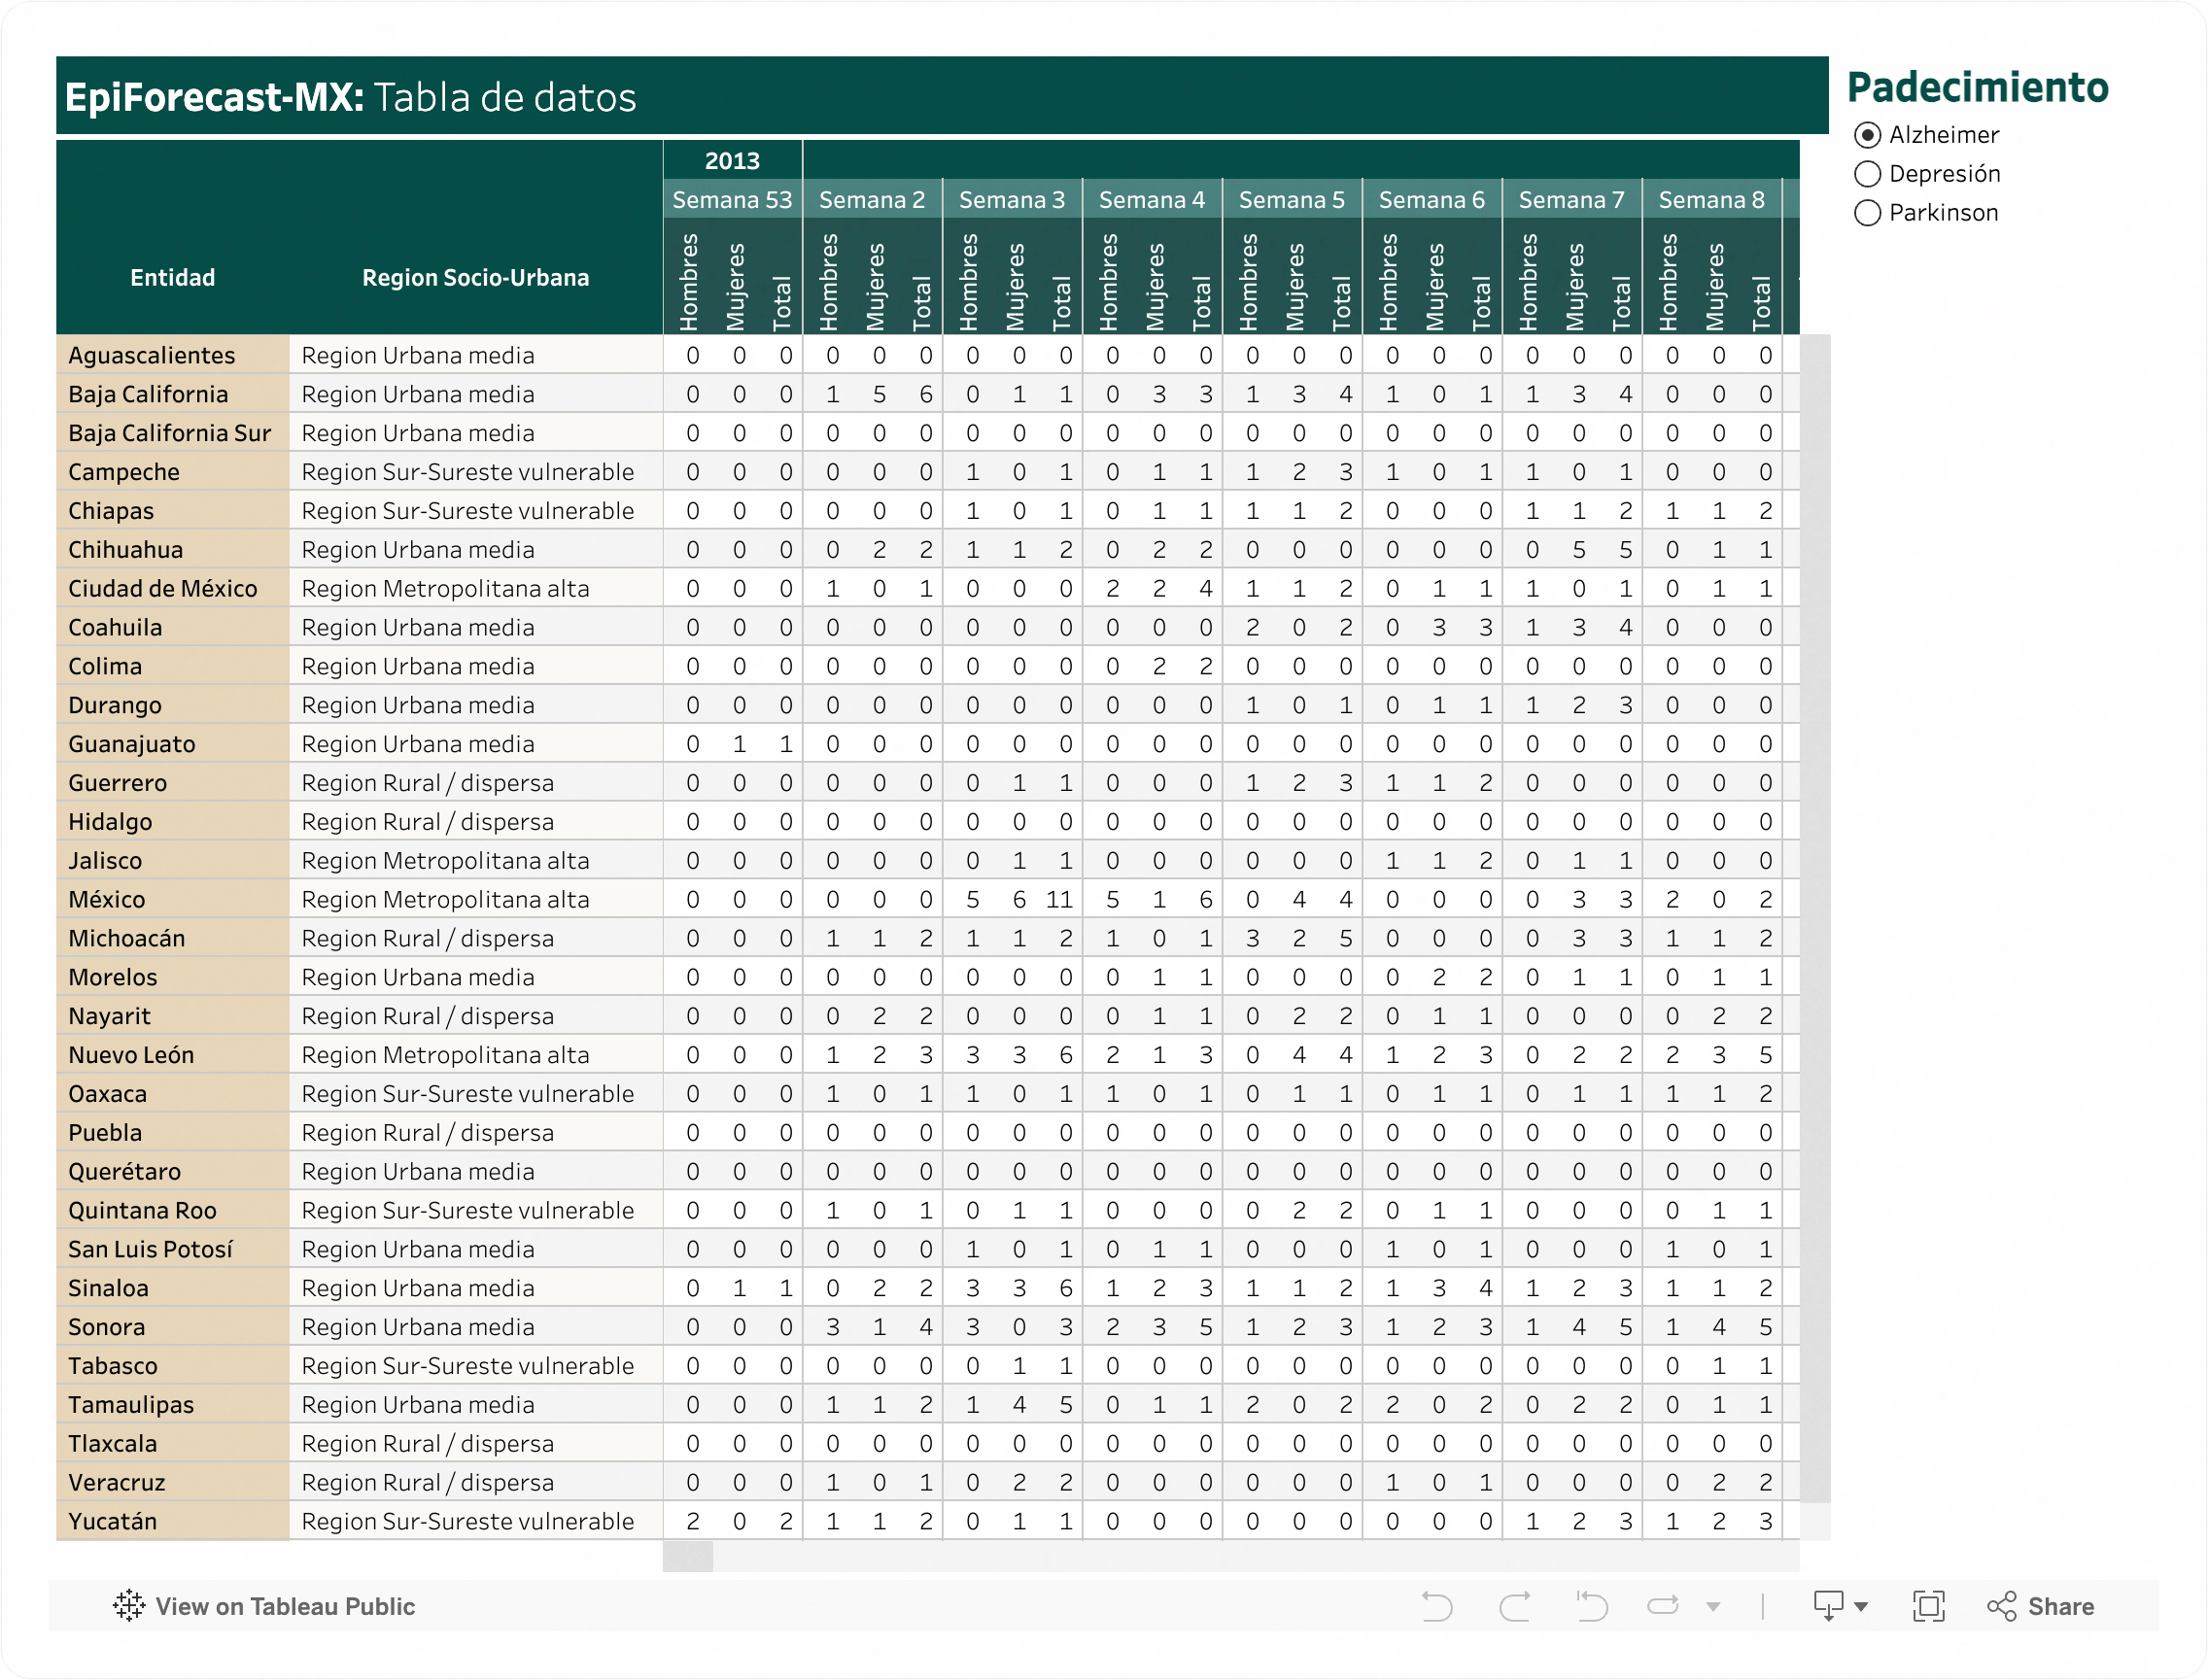
\includegraphics[width=0.80\textwidth]{explora-tabladedatos.png}
\caption[Exploración: Tabla de datos.]{Vista exploratoria \textbf{Tabla de datos}: acceso tabular al dataset consolidado; herramienta de validación y exploración detallada.}
\label{fig:web_explora_tabla}
\end{figure}

La vista \textbf{Casos por año} (\figref{fig:web_explora_casosporano}) muestra la evolución anual de la incidencia, con desagregación por padecimiento y género. Permite identificar tendencias de largo plazo, el impacto COVID-19 y la recuperación post-pandémica.

\begin{figure}[H]
\centering
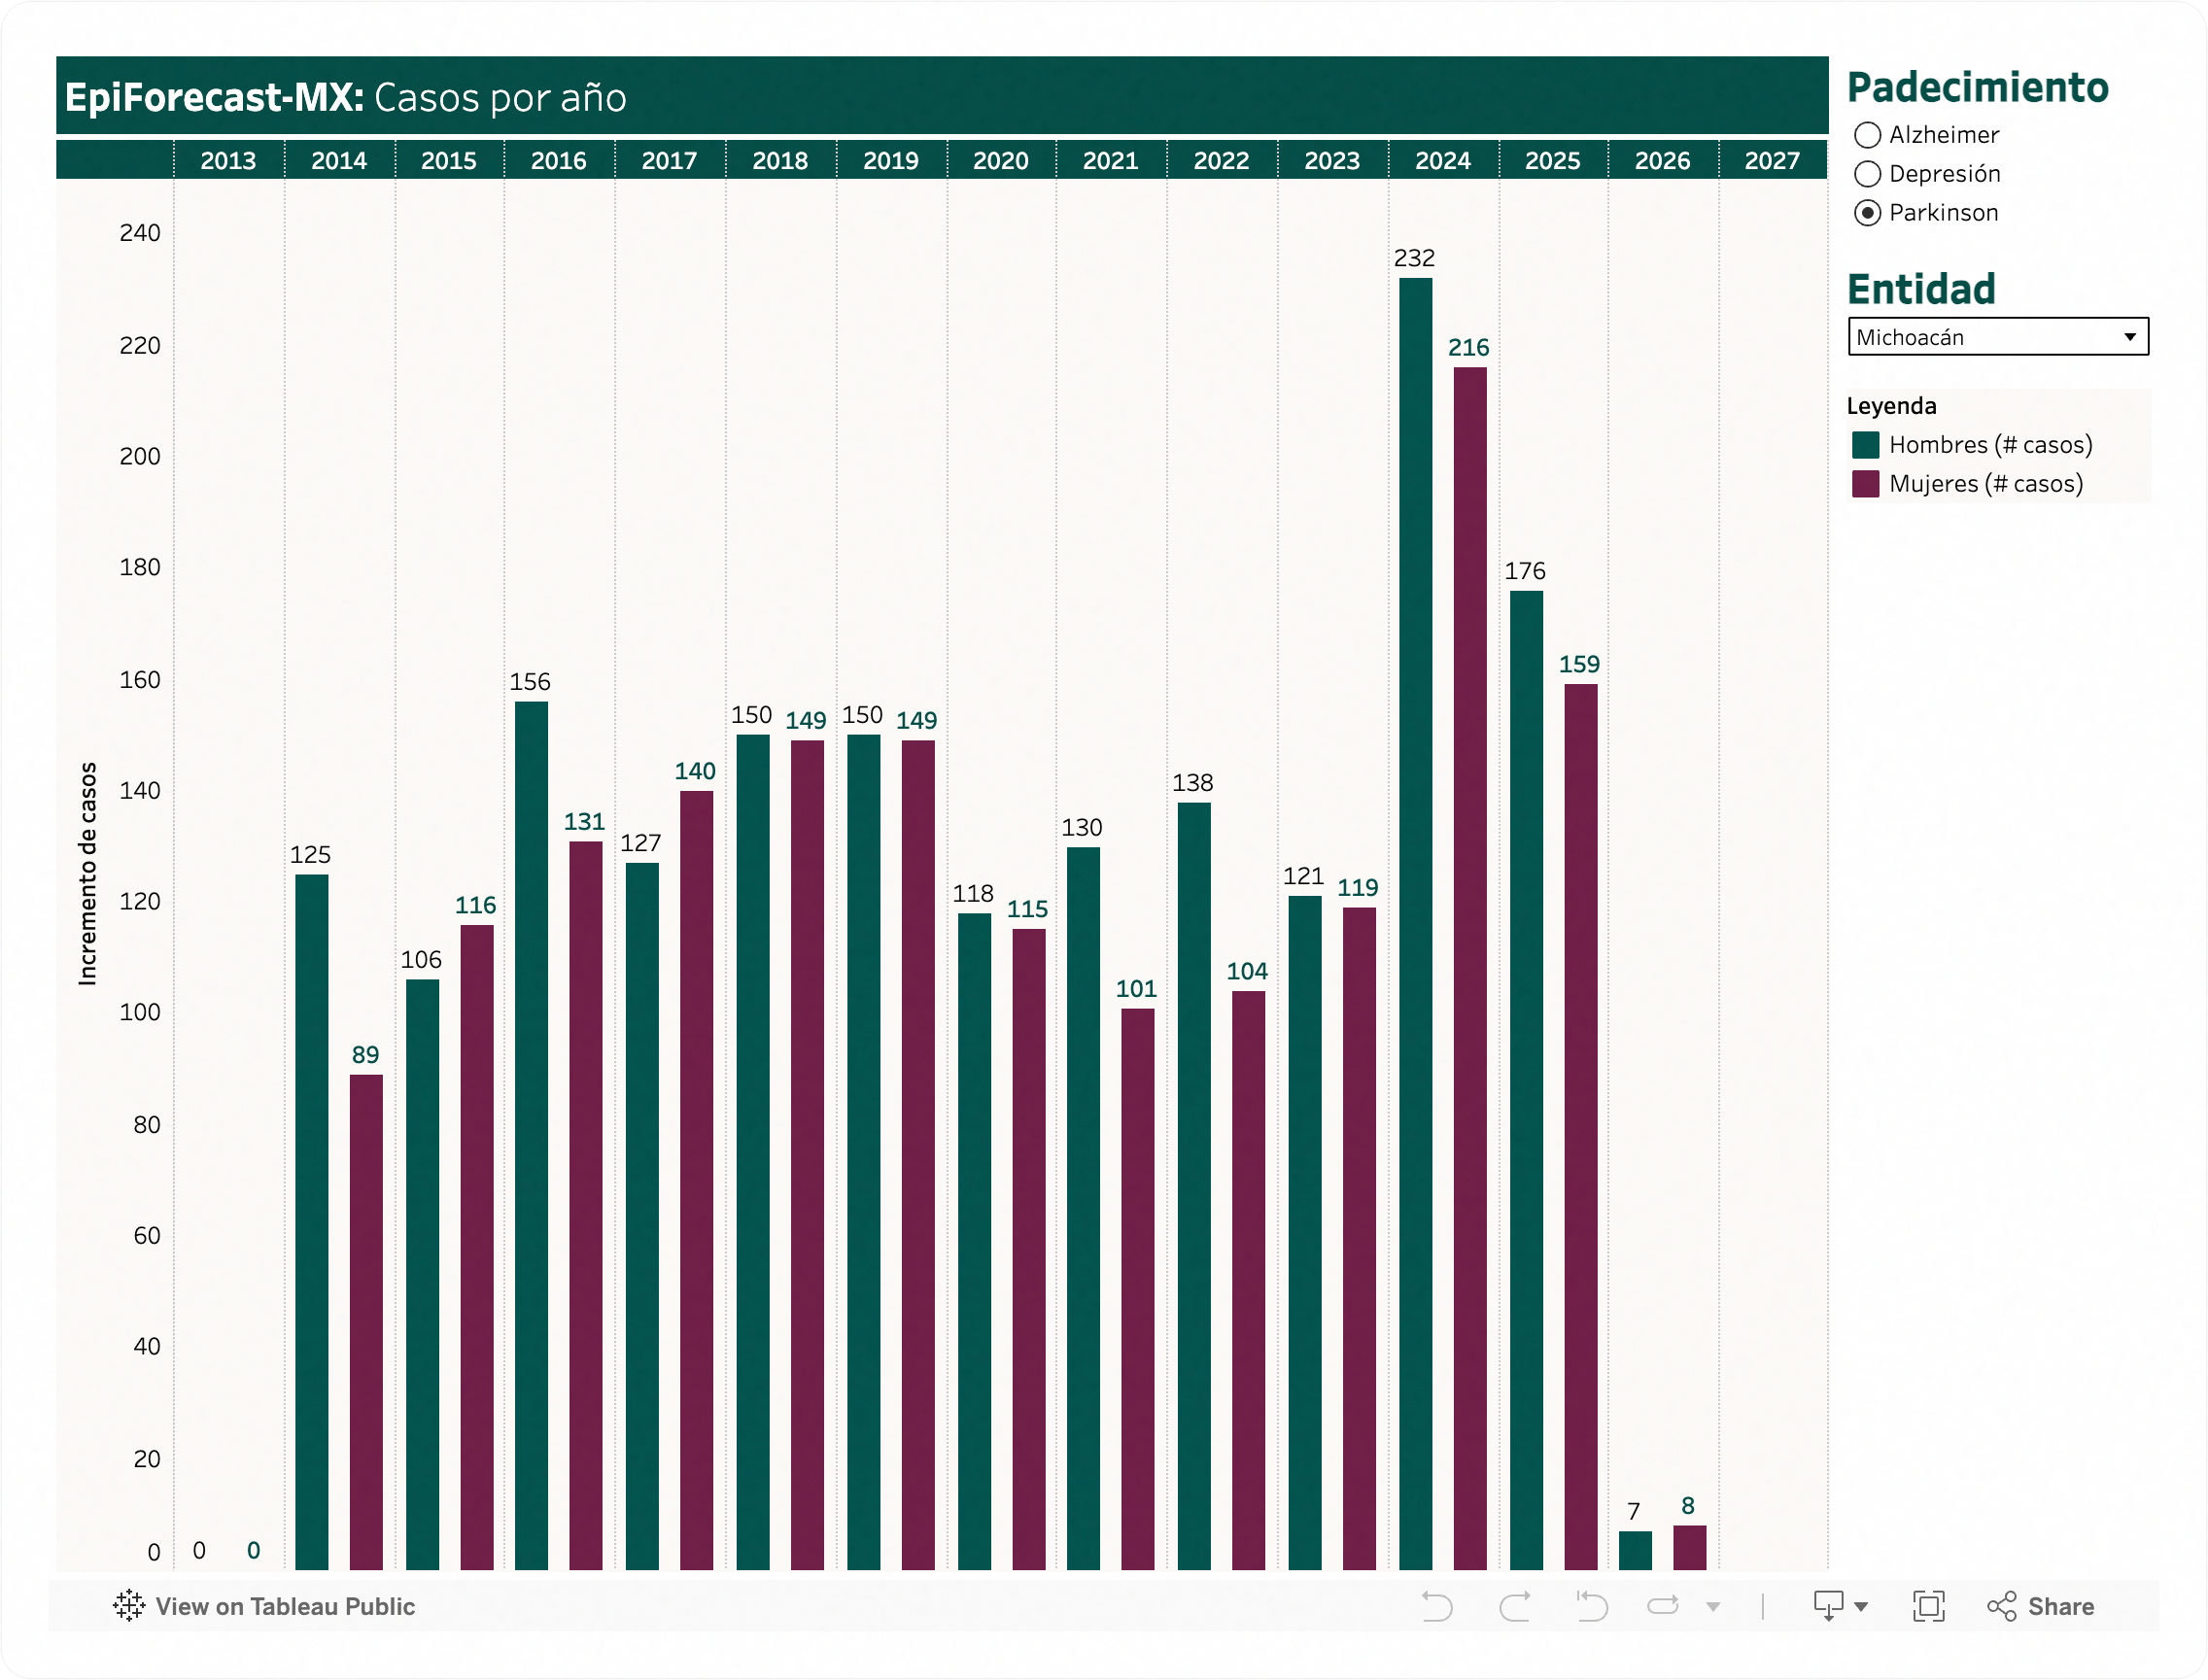
\includegraphics[width=\textwidth]{explora-casosporano.png}
\caption[Exploración: Casos por año.]{Vista exploratoria \textbf{Casos por año}: evolución anual de la incidencia normalizada por 100,000 habitantes.}
\label{fig:web_explora_casosporano}
\end{figure}

\newpage

La vista \textbf{Casos por semana} (\figref{fig:web_explora_casosporsemana}) presenta la evolución semanal del histórico completo (2014--2026), permitiendo identificar picos estacionales, cambios abruptos y la estacionalidad suave de Parkinson.

\begin{figure}[H]
\centering
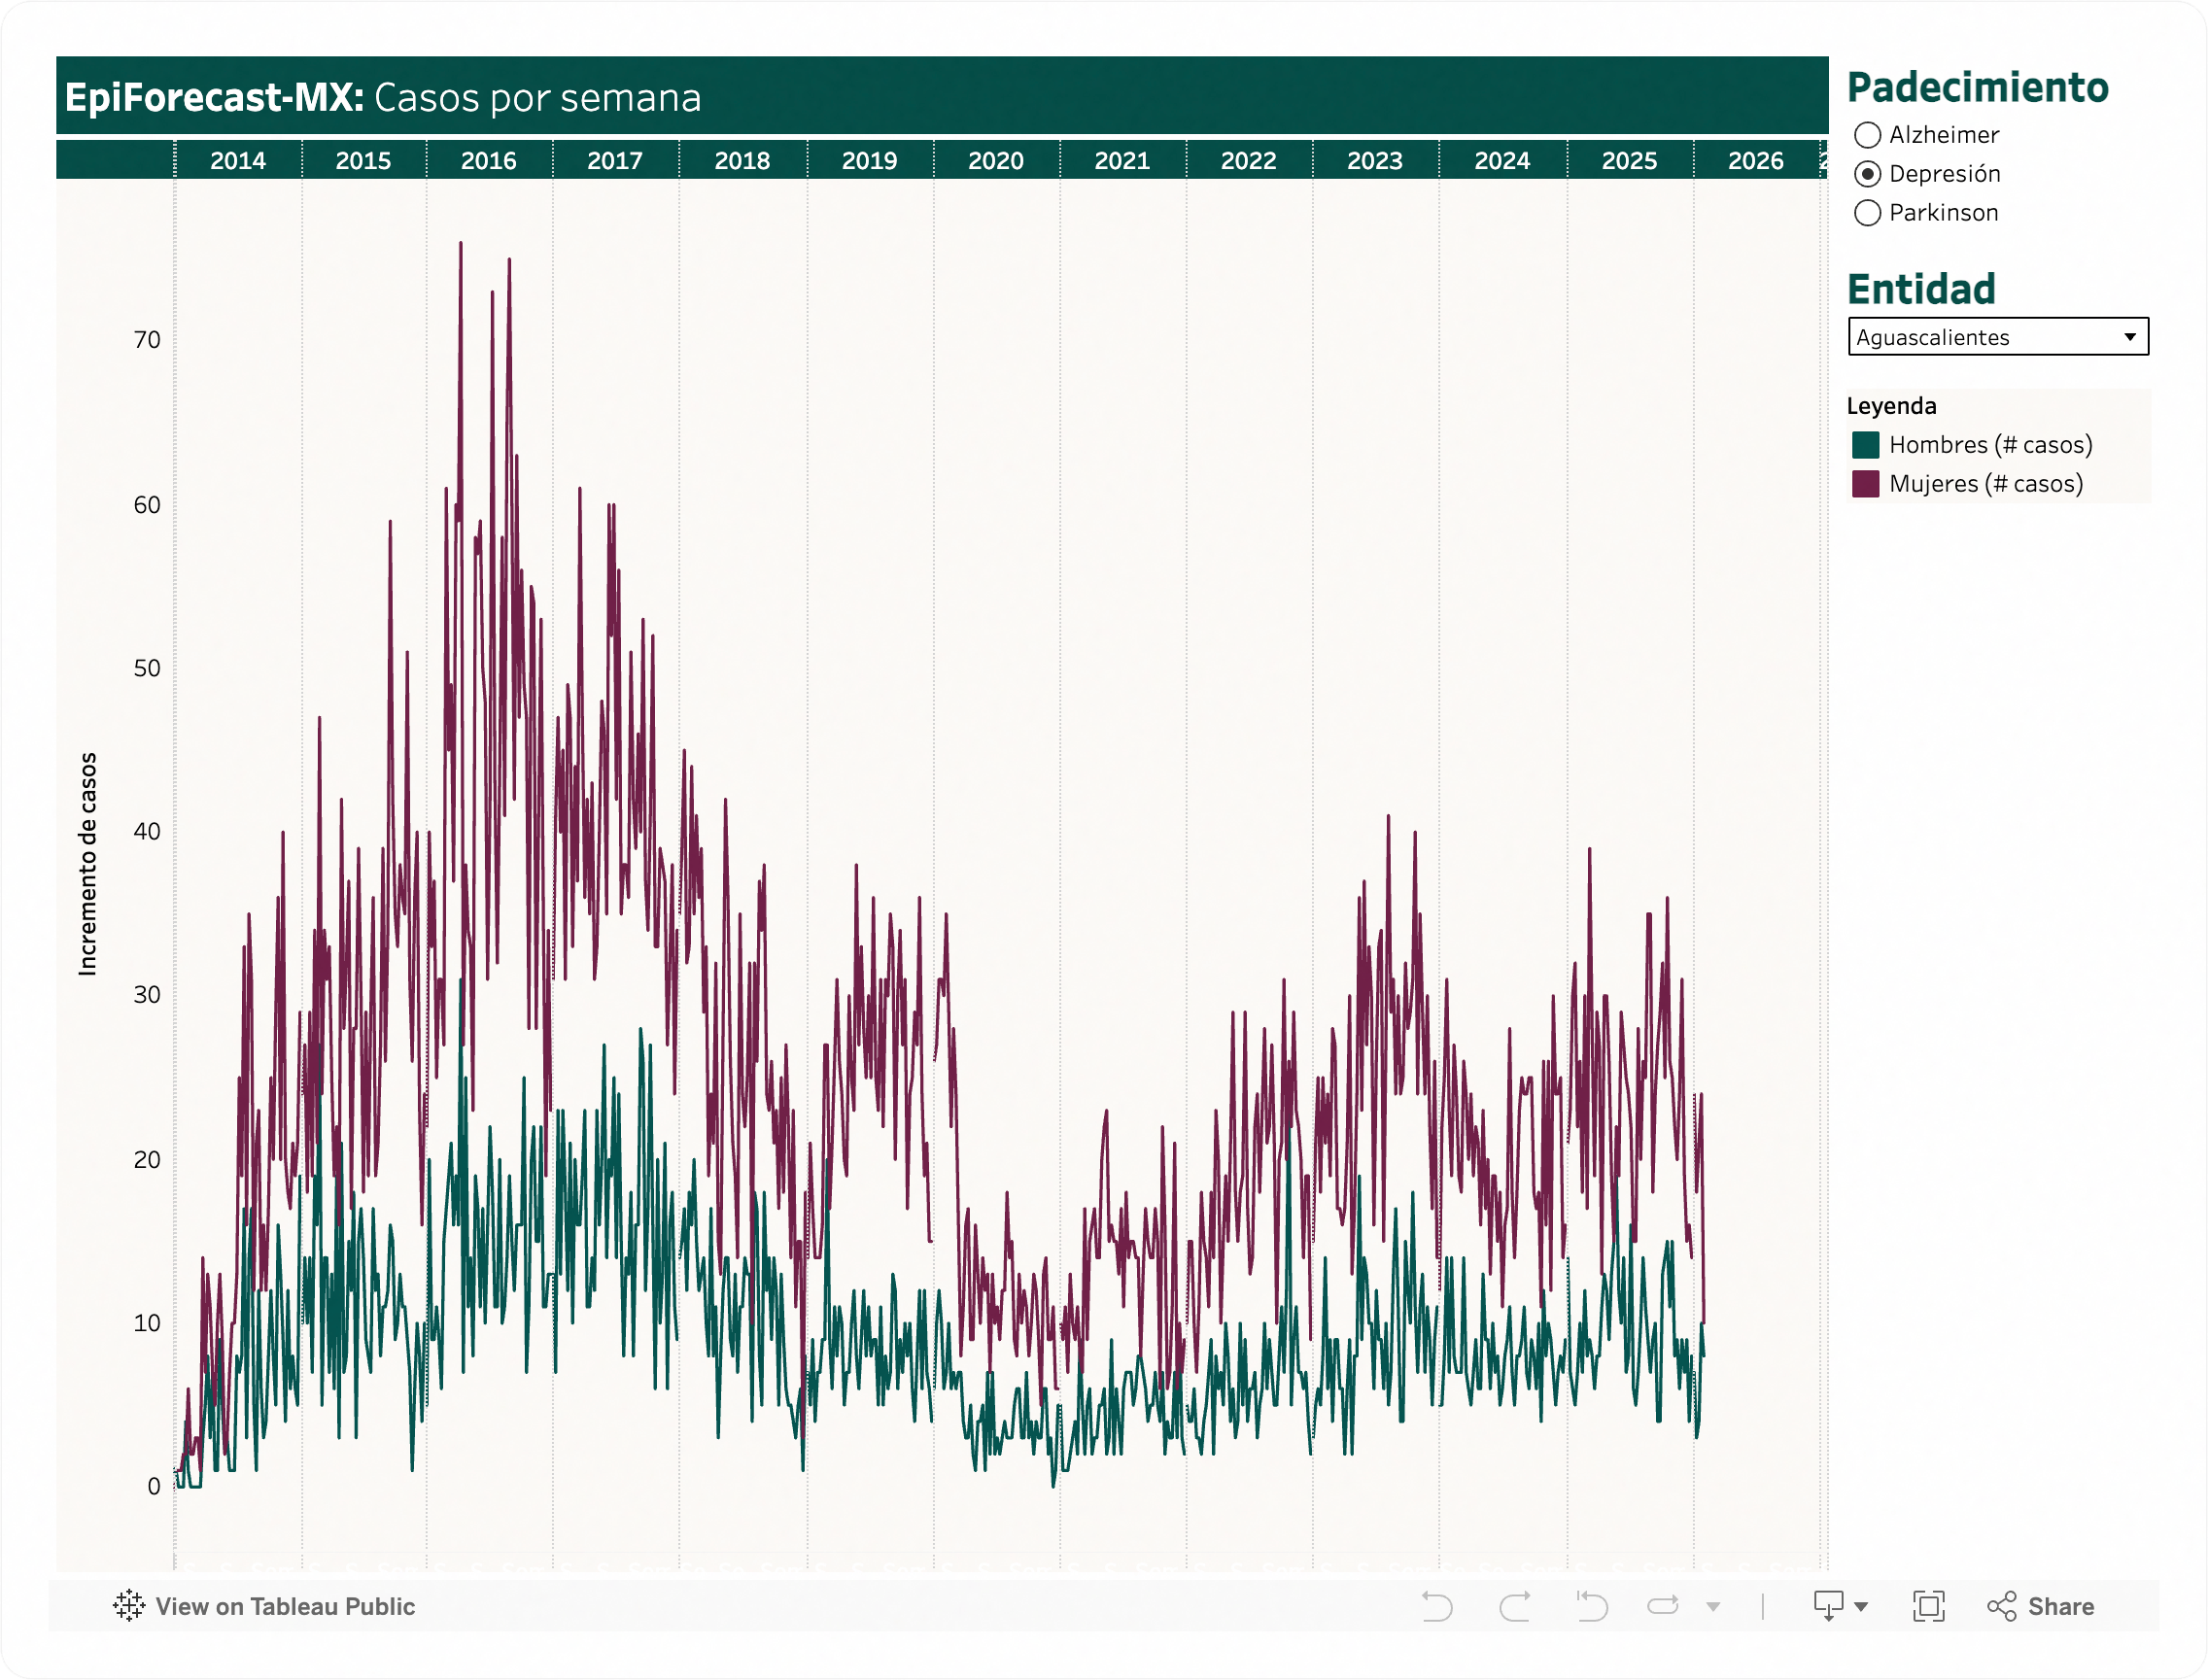
\includegraphics[width=\textwidth]{explora-casosporsemana.png}
\caption[Exploración: Casos por semana.]{Vista exploratoria \textbf{Casos por semana}: evolución semanal de la incidencia; identifica picos, estacionalidad y el impacto de COVID-19.}
\label{fig:web_explora_casosporsemana}
\end{figure}

La vista \textbf{Mapa de México} (\figref{fig:web_explora_mapa}) ofrece una representación geográfica coroplética de la incidencia y variables demográficas del \textsc{inegi} por entidad federativa. Al hacer clic sobre cualquier entidad, el mapa actúa como filtro de contexto que actualiza las demás vistas del dashboard.

\begin{figure}[H]
\centering
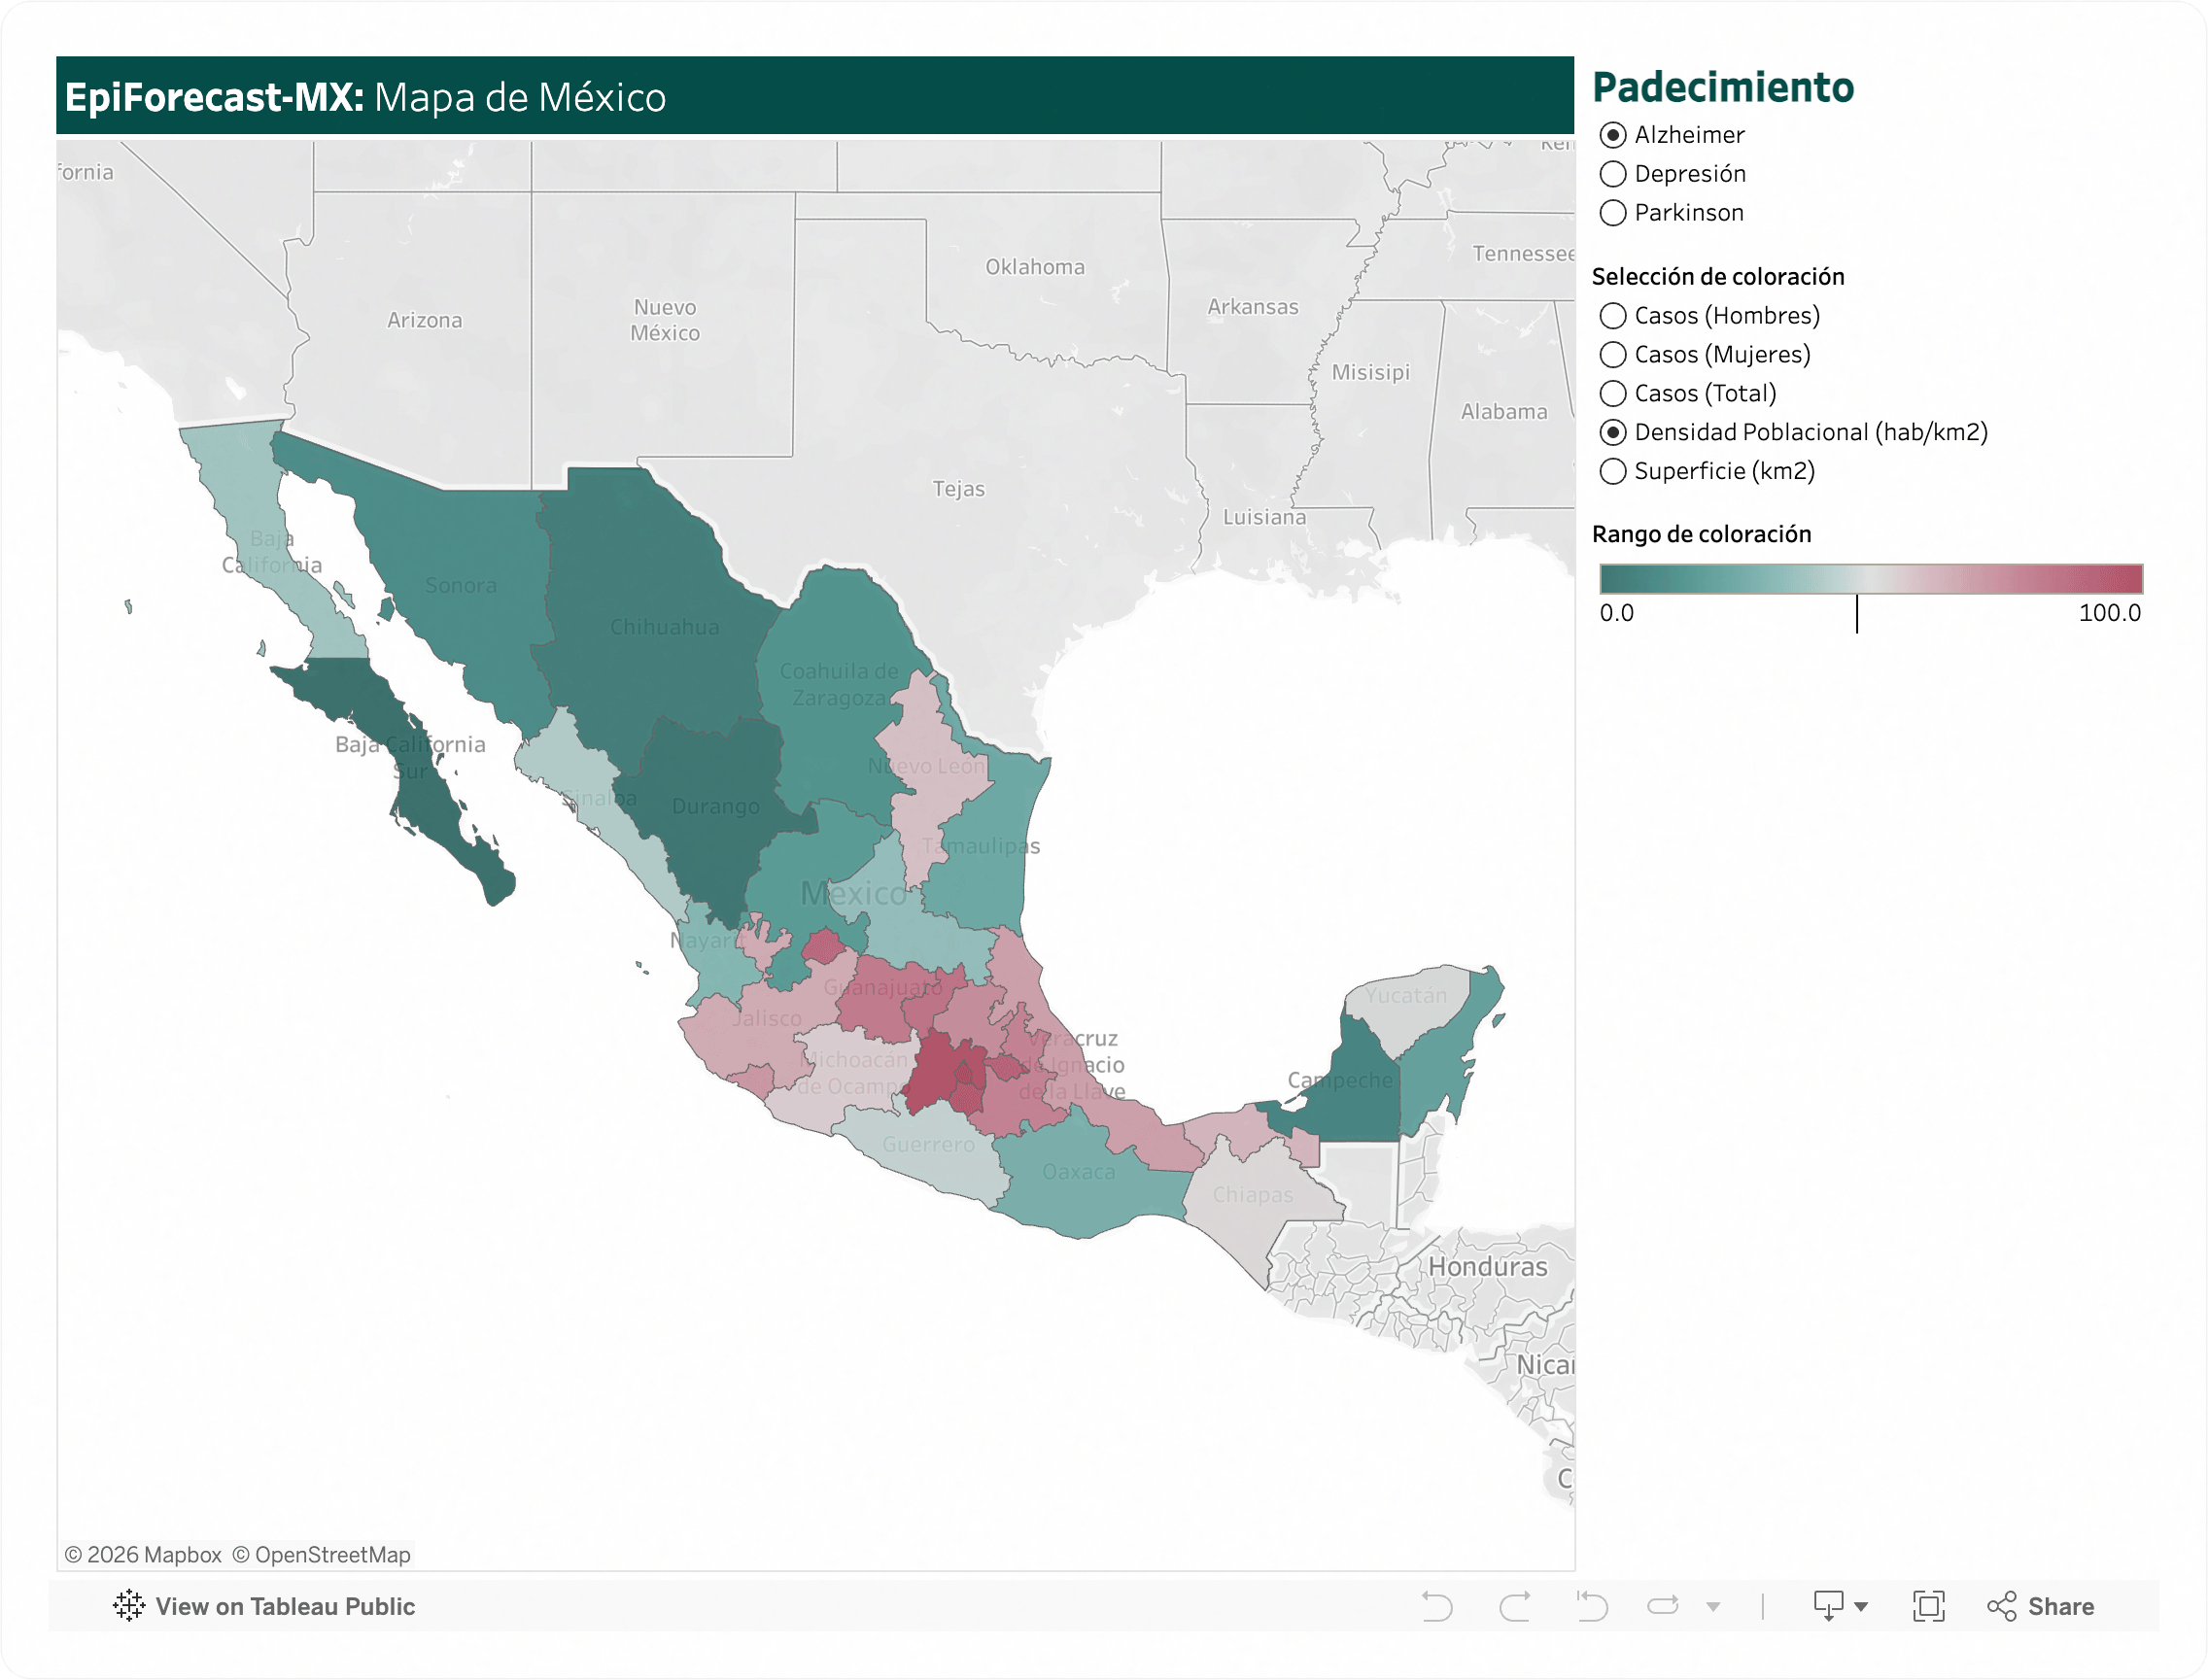
\includegraphics[width=\textwidth]{explora-mapademexico.png}
\caption[Exploración: Mapa de México.]{Vista exploratoria \textbf{Mapa de México}: representación geográfica coroplética por entidad federativa.}
\label{fig:web_explora_mapa}
\end{figure}

\newpage

La vista \textbf{México en categorías} (\figref{fig:web_explora_categorias}) clasifica las 32 entidades según atributos territoriales del \textsc{inegi}: región socioeconómica, densidad poblacional, superficie y ratio hombres-mujeres. Provee el contexto demográfico para interpretar diferencias de rendimiento entre series.

\begin{figure}[H]
\centering
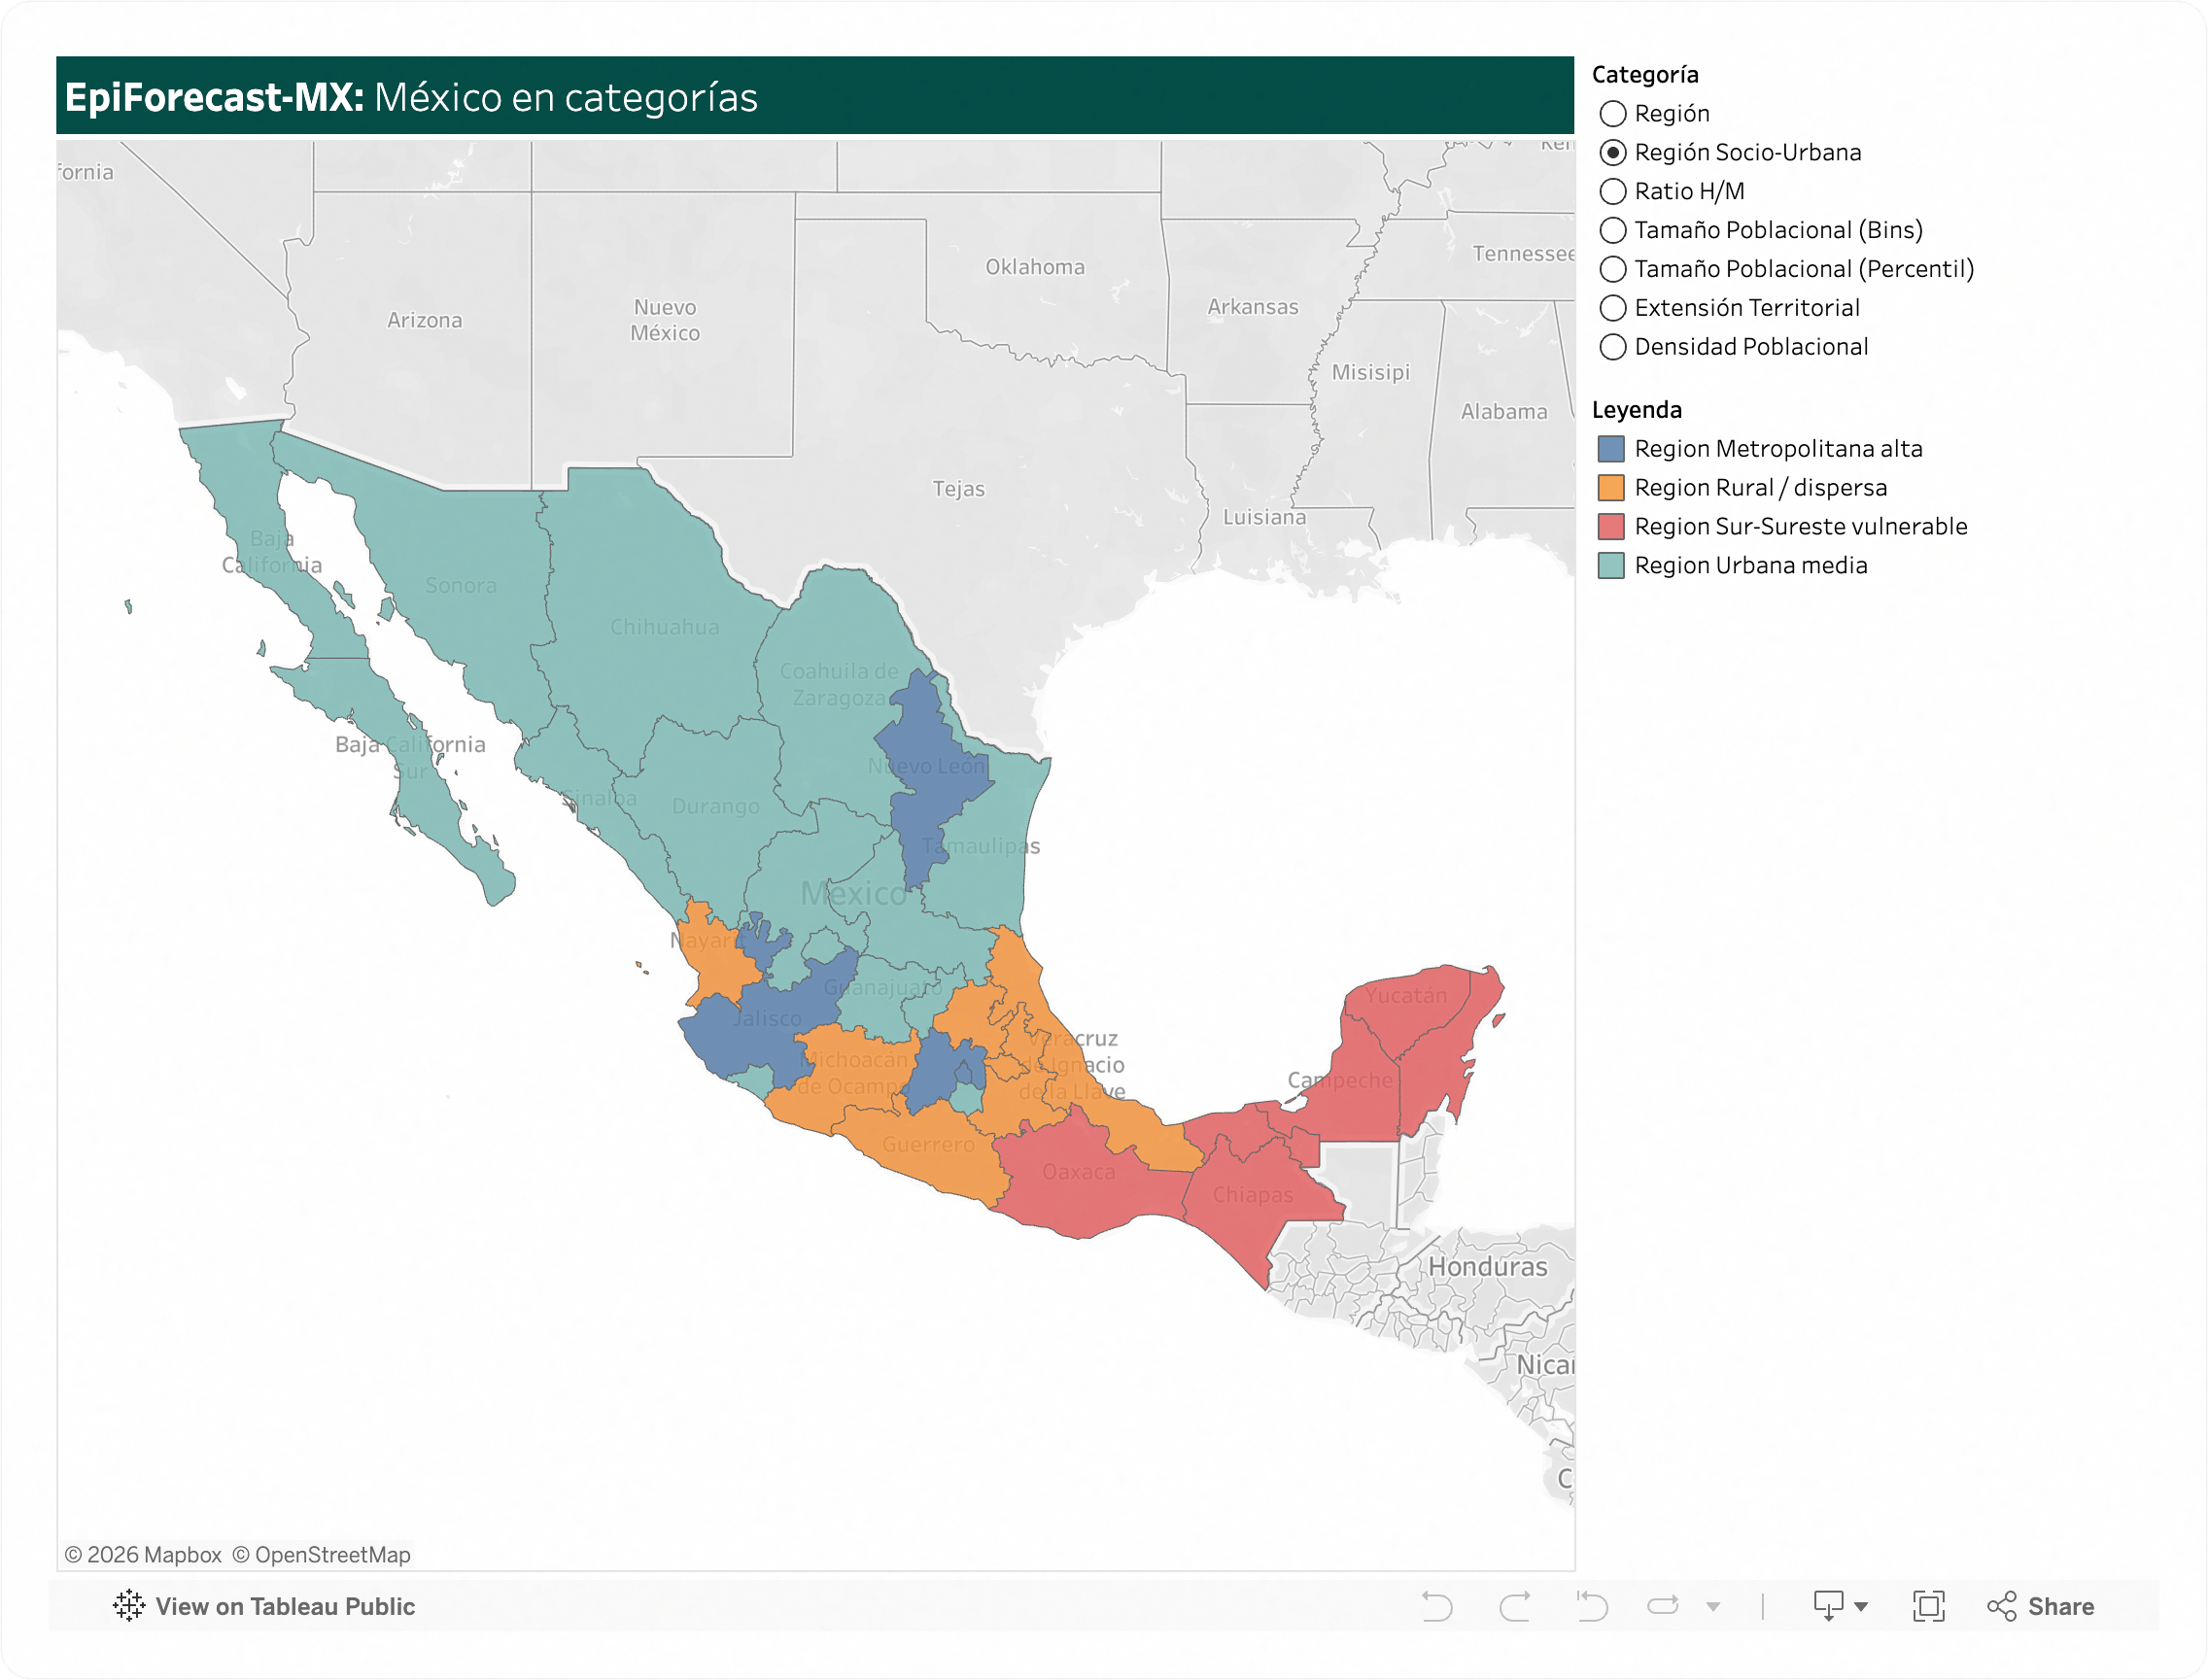
\includegraphics[width=\textwidth]{explora-mexicoencategorias.png}
\caption[Exploración: México en categorías.]{Vista exploratoria \textbf{México en categorías}: clasificación territorial de las 32 entidades.}
\label{fig:web_explora_categorias}
\end{figure}

\subsubsection{Vistas de predicción}

La vista \textbf{Predicción estatal con intervalo de confianza} (\figref{fig:web_prediccion_estatal_banda}) es la visualización de mayor valor analítico para el epidemiólogo delegacional. Muestra el pronóstico a 52 semanas con bandas de confianza al 80\%. Una banda estrecha refleja alta certeza del modelo; una banda ancha indica mayor incertidumbre.

\begin{figure}[H]
\centering
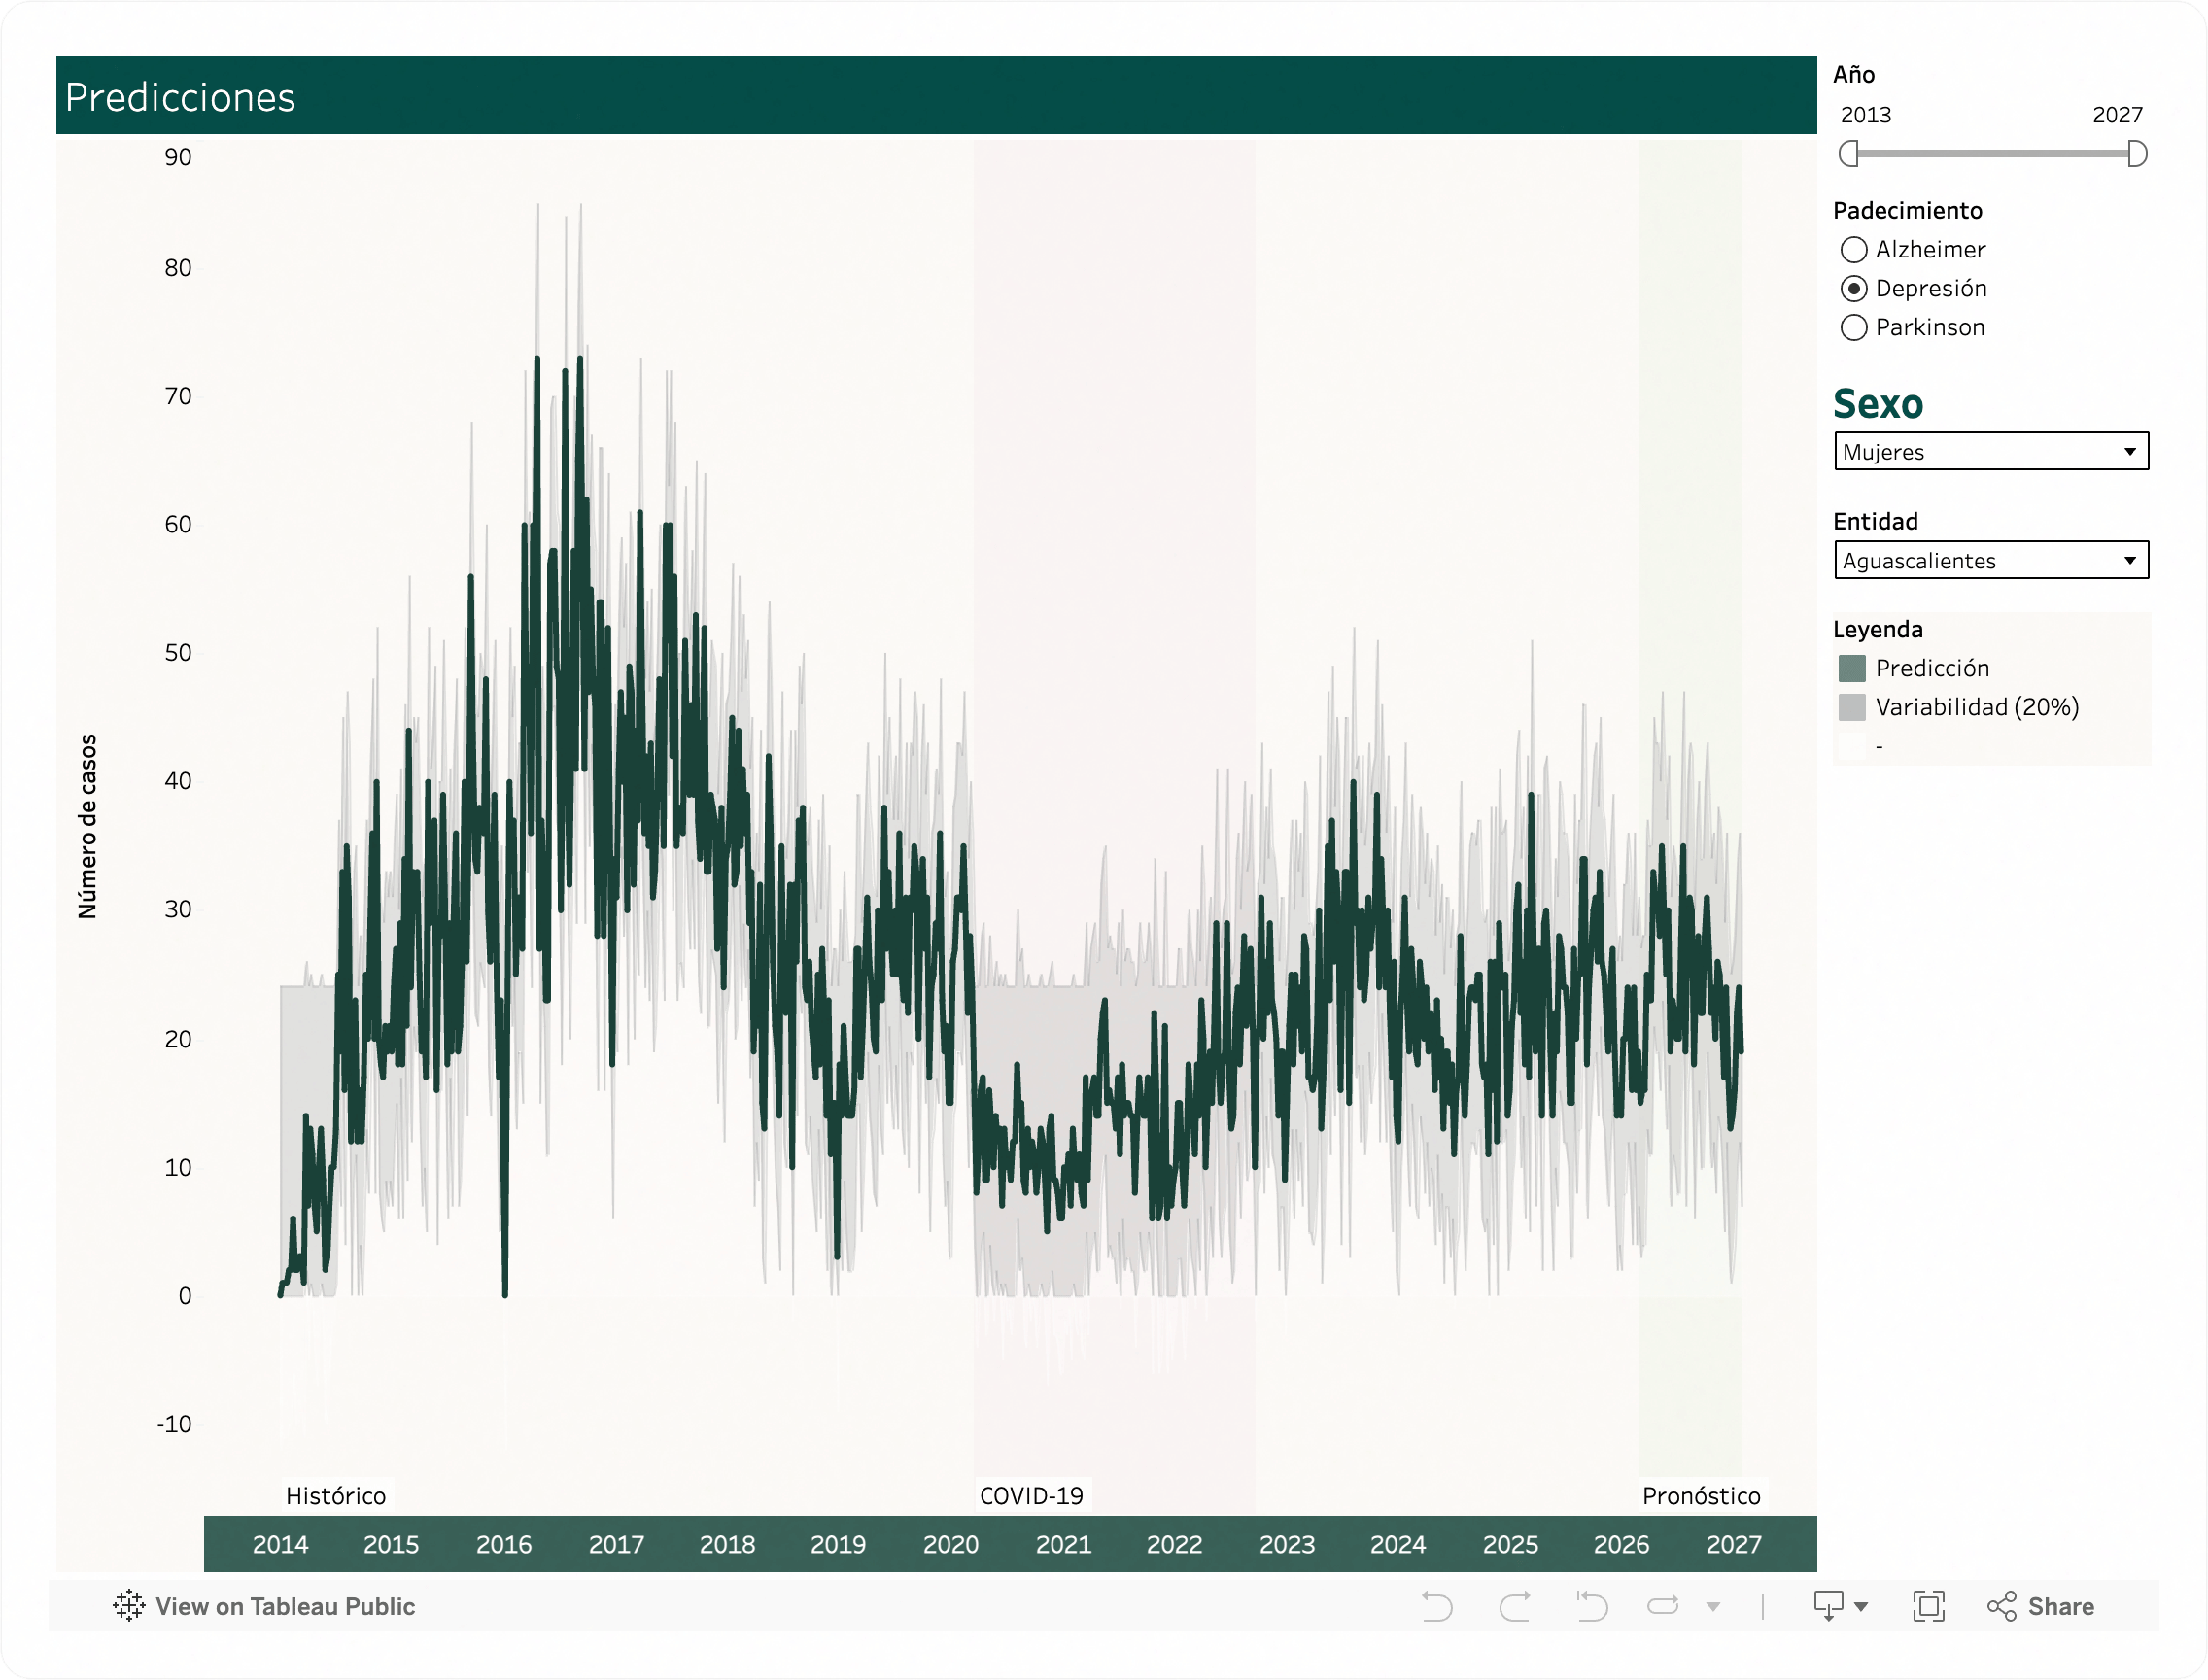
\includegraphics[width=\textwidth]{prediccion-estatal-banda.png}
\caption[Predicción estatal con intervalo de confianza.]{Vista \textbf{Predicción estatal con intervalo de confianza}: pronóstico a 52 semanas por entidad con bandas al 80\%.}
\label{fig:web_prediccion_estatal_banda}
\end{figure}

\newpage

La vista \textbf{Predicción estatal} (\figref{fig:web_prediccion_estatal}) presenta la serie histórica completa y el pronóstico sin bandas de confianza, diseñada para comunicar el pronóstico a perfiles no técnicos.

\begin{figure}[H]
\centering
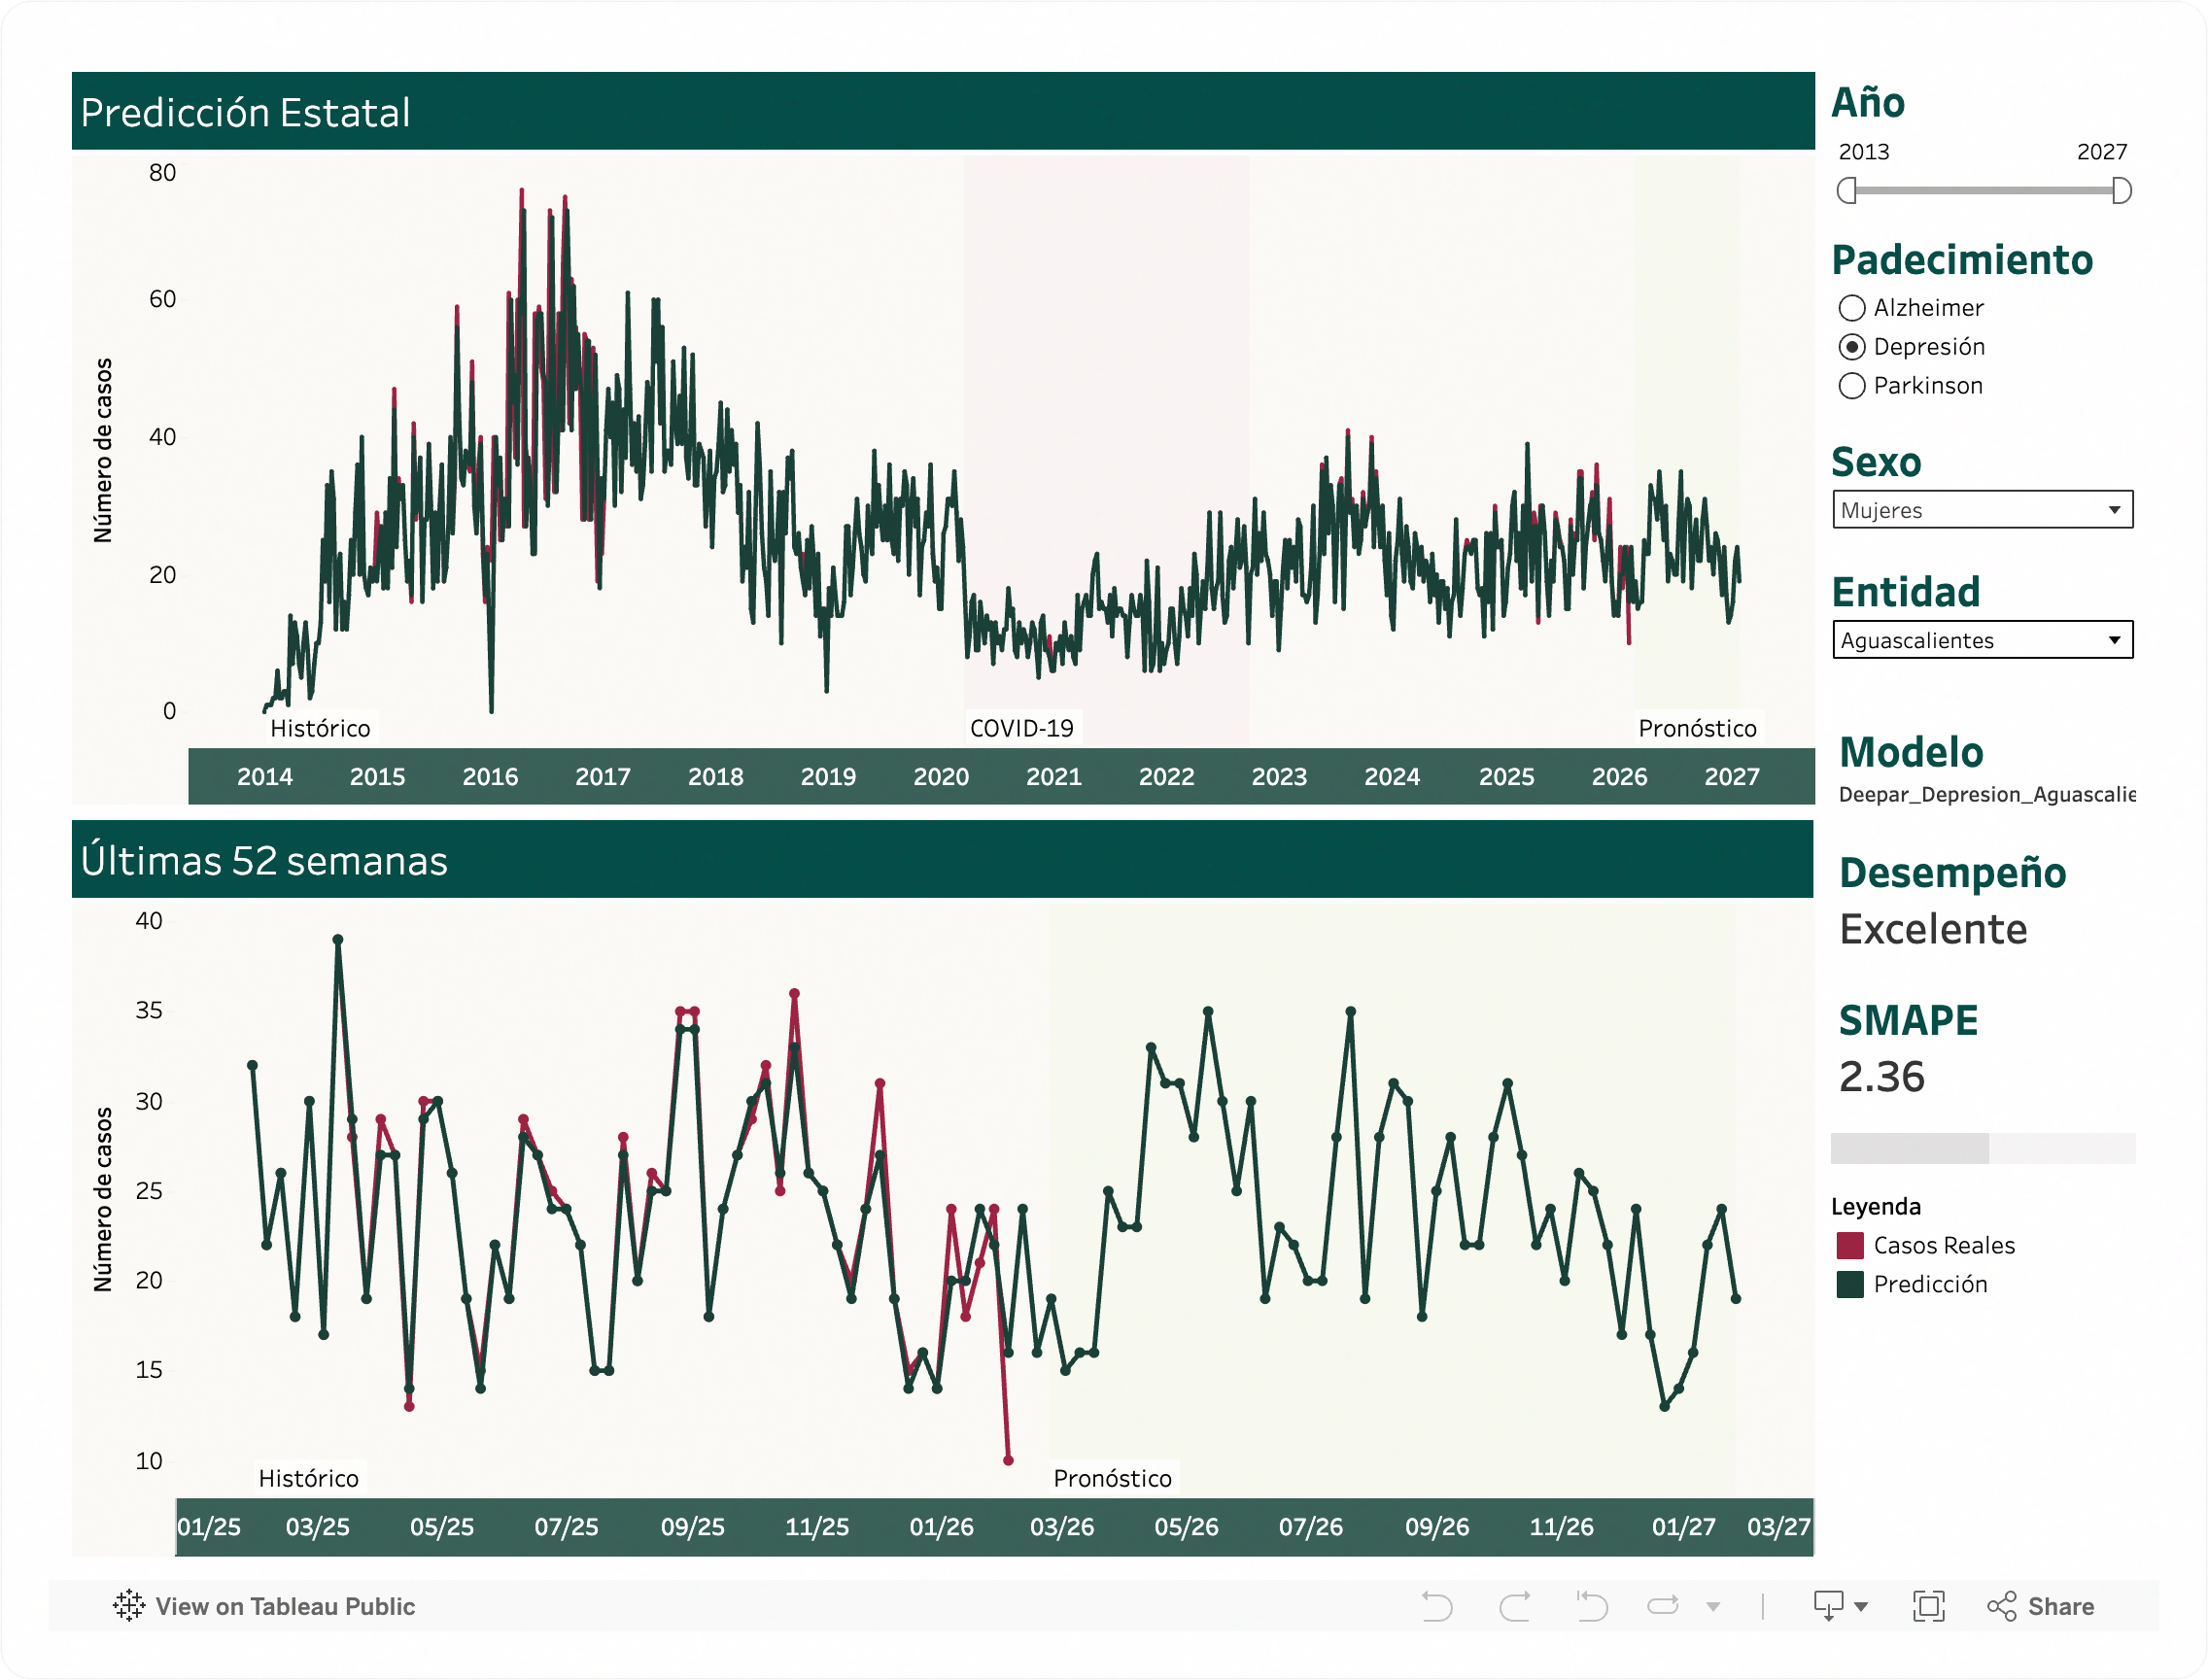
\includegraphics[width=\textwidth]{prediccion-estatal.png}
\caption[Predicción estatal.]{Vista \textbf{Predicción estatal}: serie histórica y pronóstico a 52 semanas por entidad federativa.}
\label{fig:web_prediccion_estatal}
\end{figure}

La vista \textbf{Predicción nacional} (\figref{fig:web_prediccion_nacional}) es el punto de entrada principal del \textbf{DashNacional}. Muestra la serie temporal completa desde 2014 hasta 2027, integrando histórico, pronóstico a 52 semanas y la franja COVID-19 sombreada.

\begin{figure}[H]
\centering
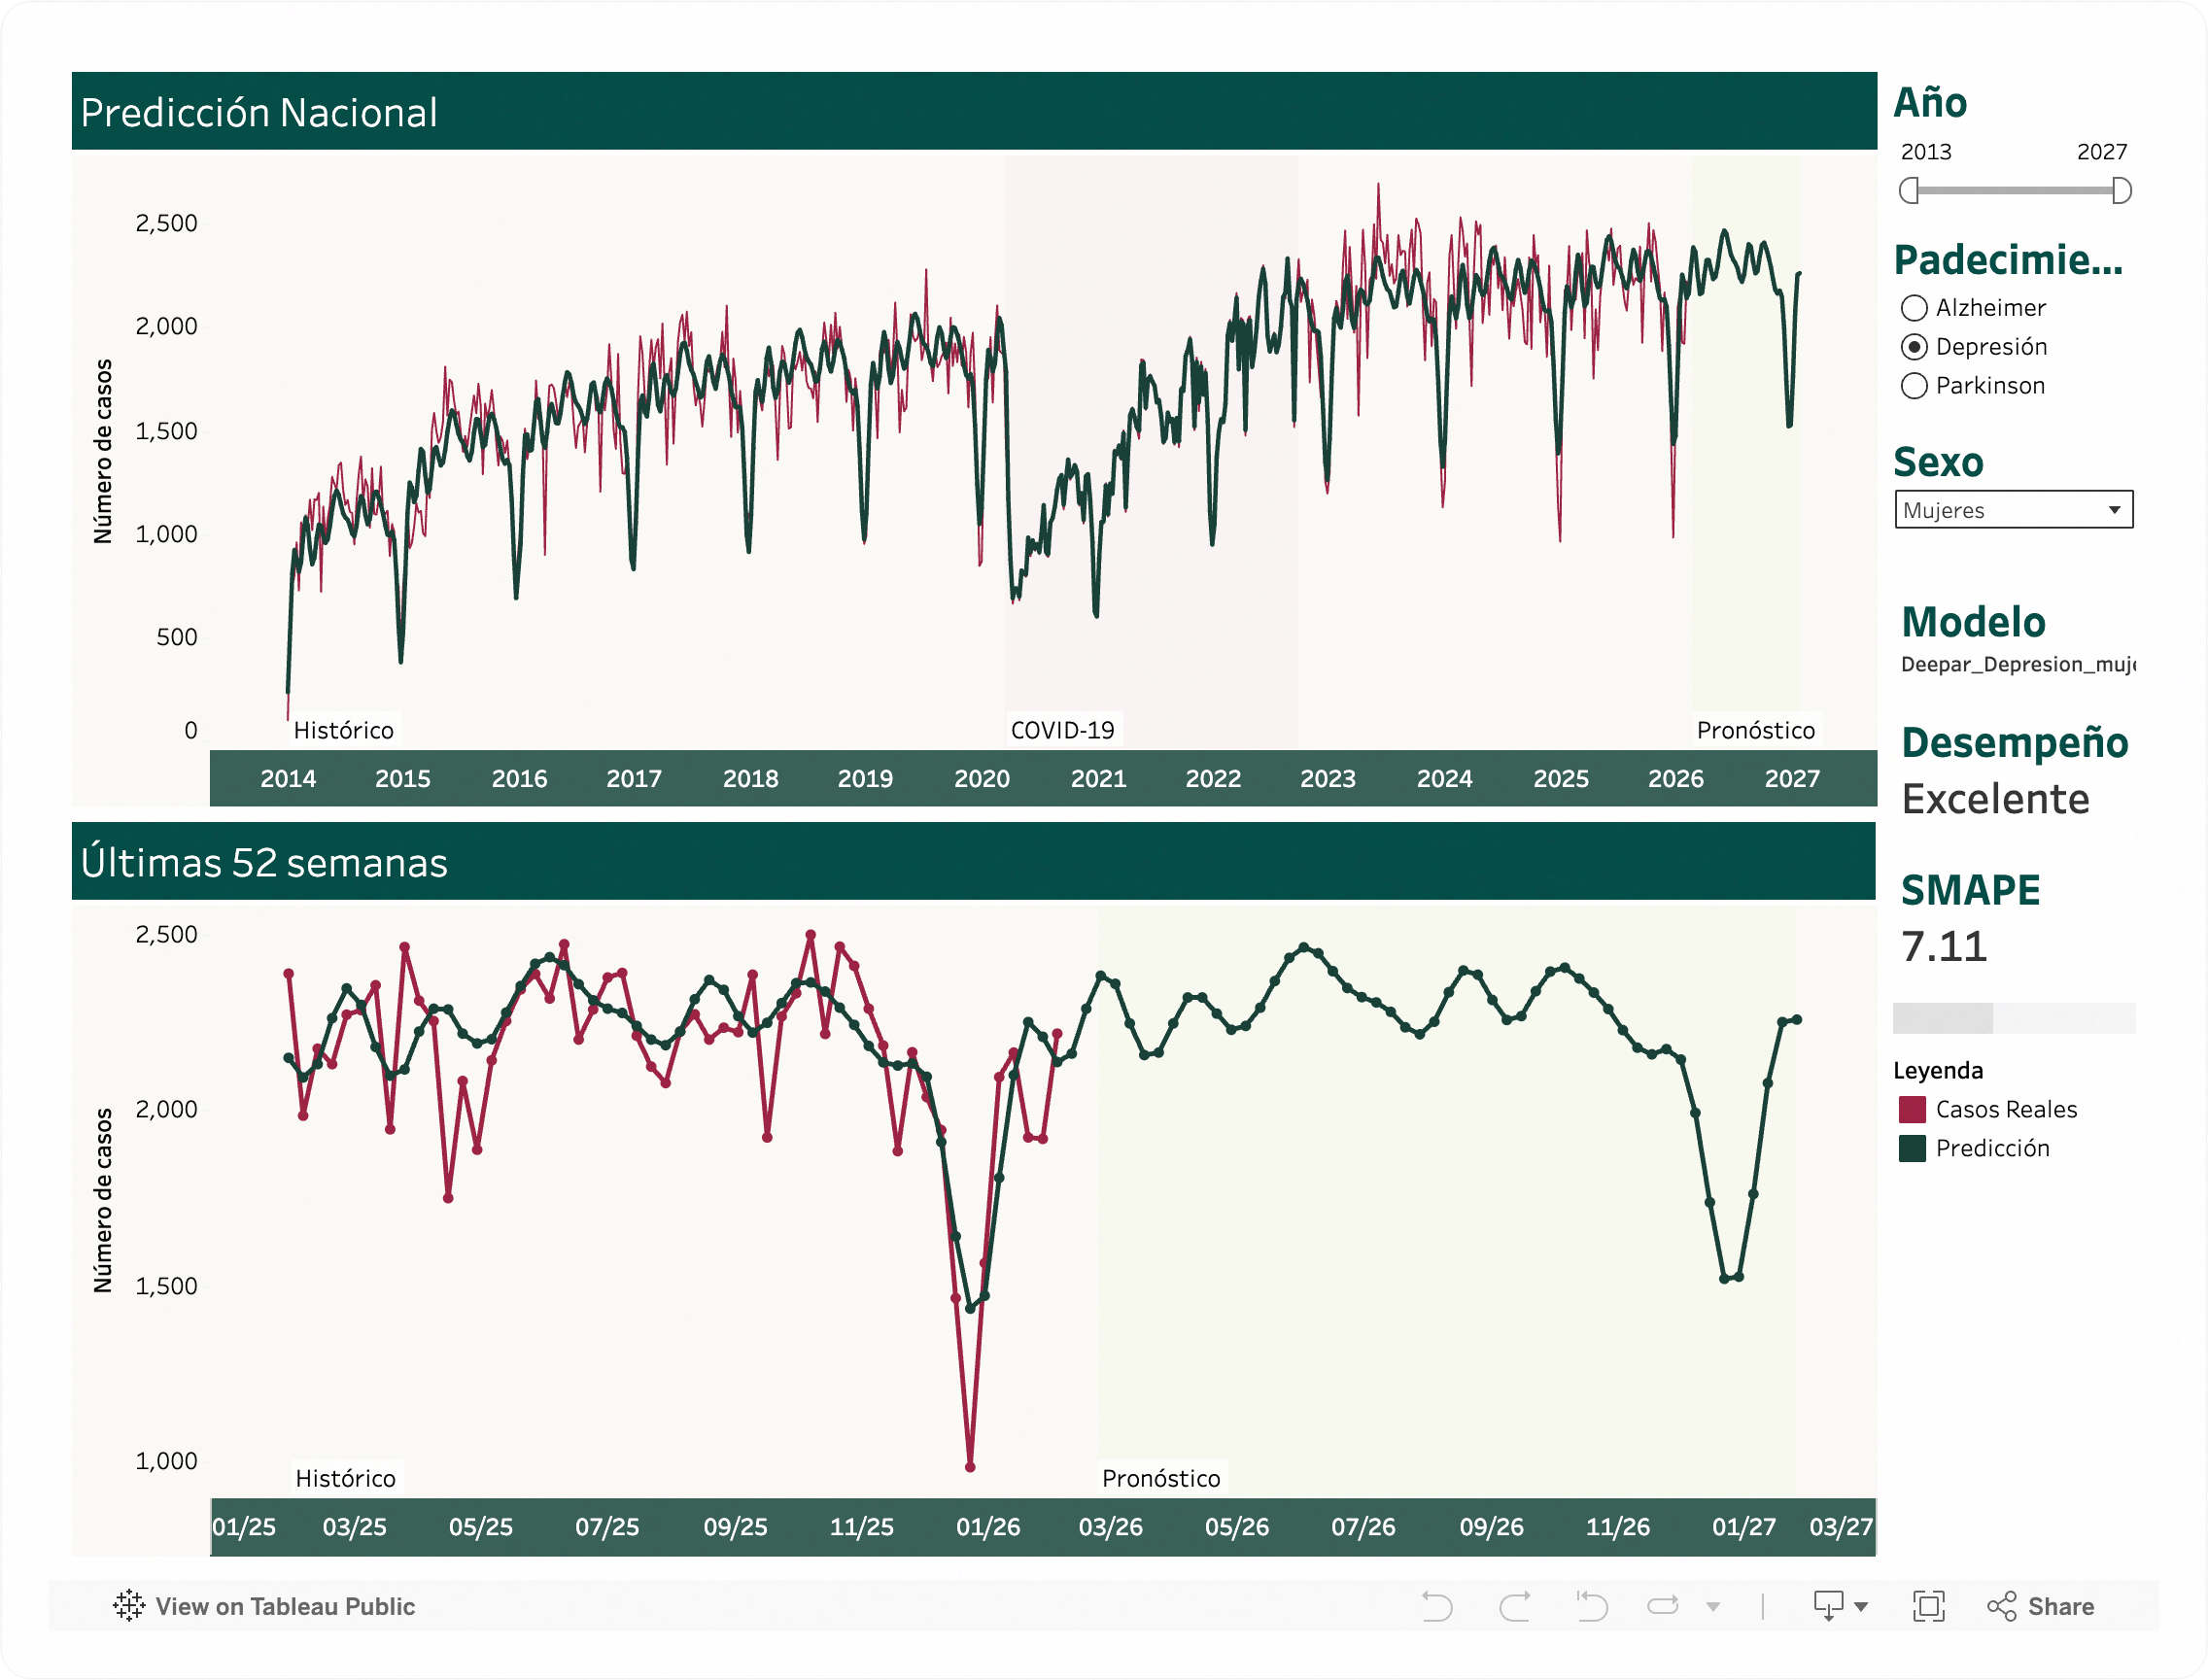
\includegraphics[width=\textwidth]{prediccion-nacional.png}
\caption[Predicción nacional.]{Vista \textbf{Predicción nacional}: serie temporal completa 2014--2027 con pronóstico a 52 semanas, zona COVID-19 sombreada y métricas del modelo activo.}
\label{fig:web_prediccion_nacional}
\end{figure}

\newpage

La vista \textbf{Predicción regional} (\figref{fig:web_prediccion_regional}) compara simultáneamente las tendencias y pronósticos de las cuatro regiones de salud mental en un mismo eje, identificando divergencias macrorregionales no visibles a nivel nacional.

\begin{figure}[H]
\centering
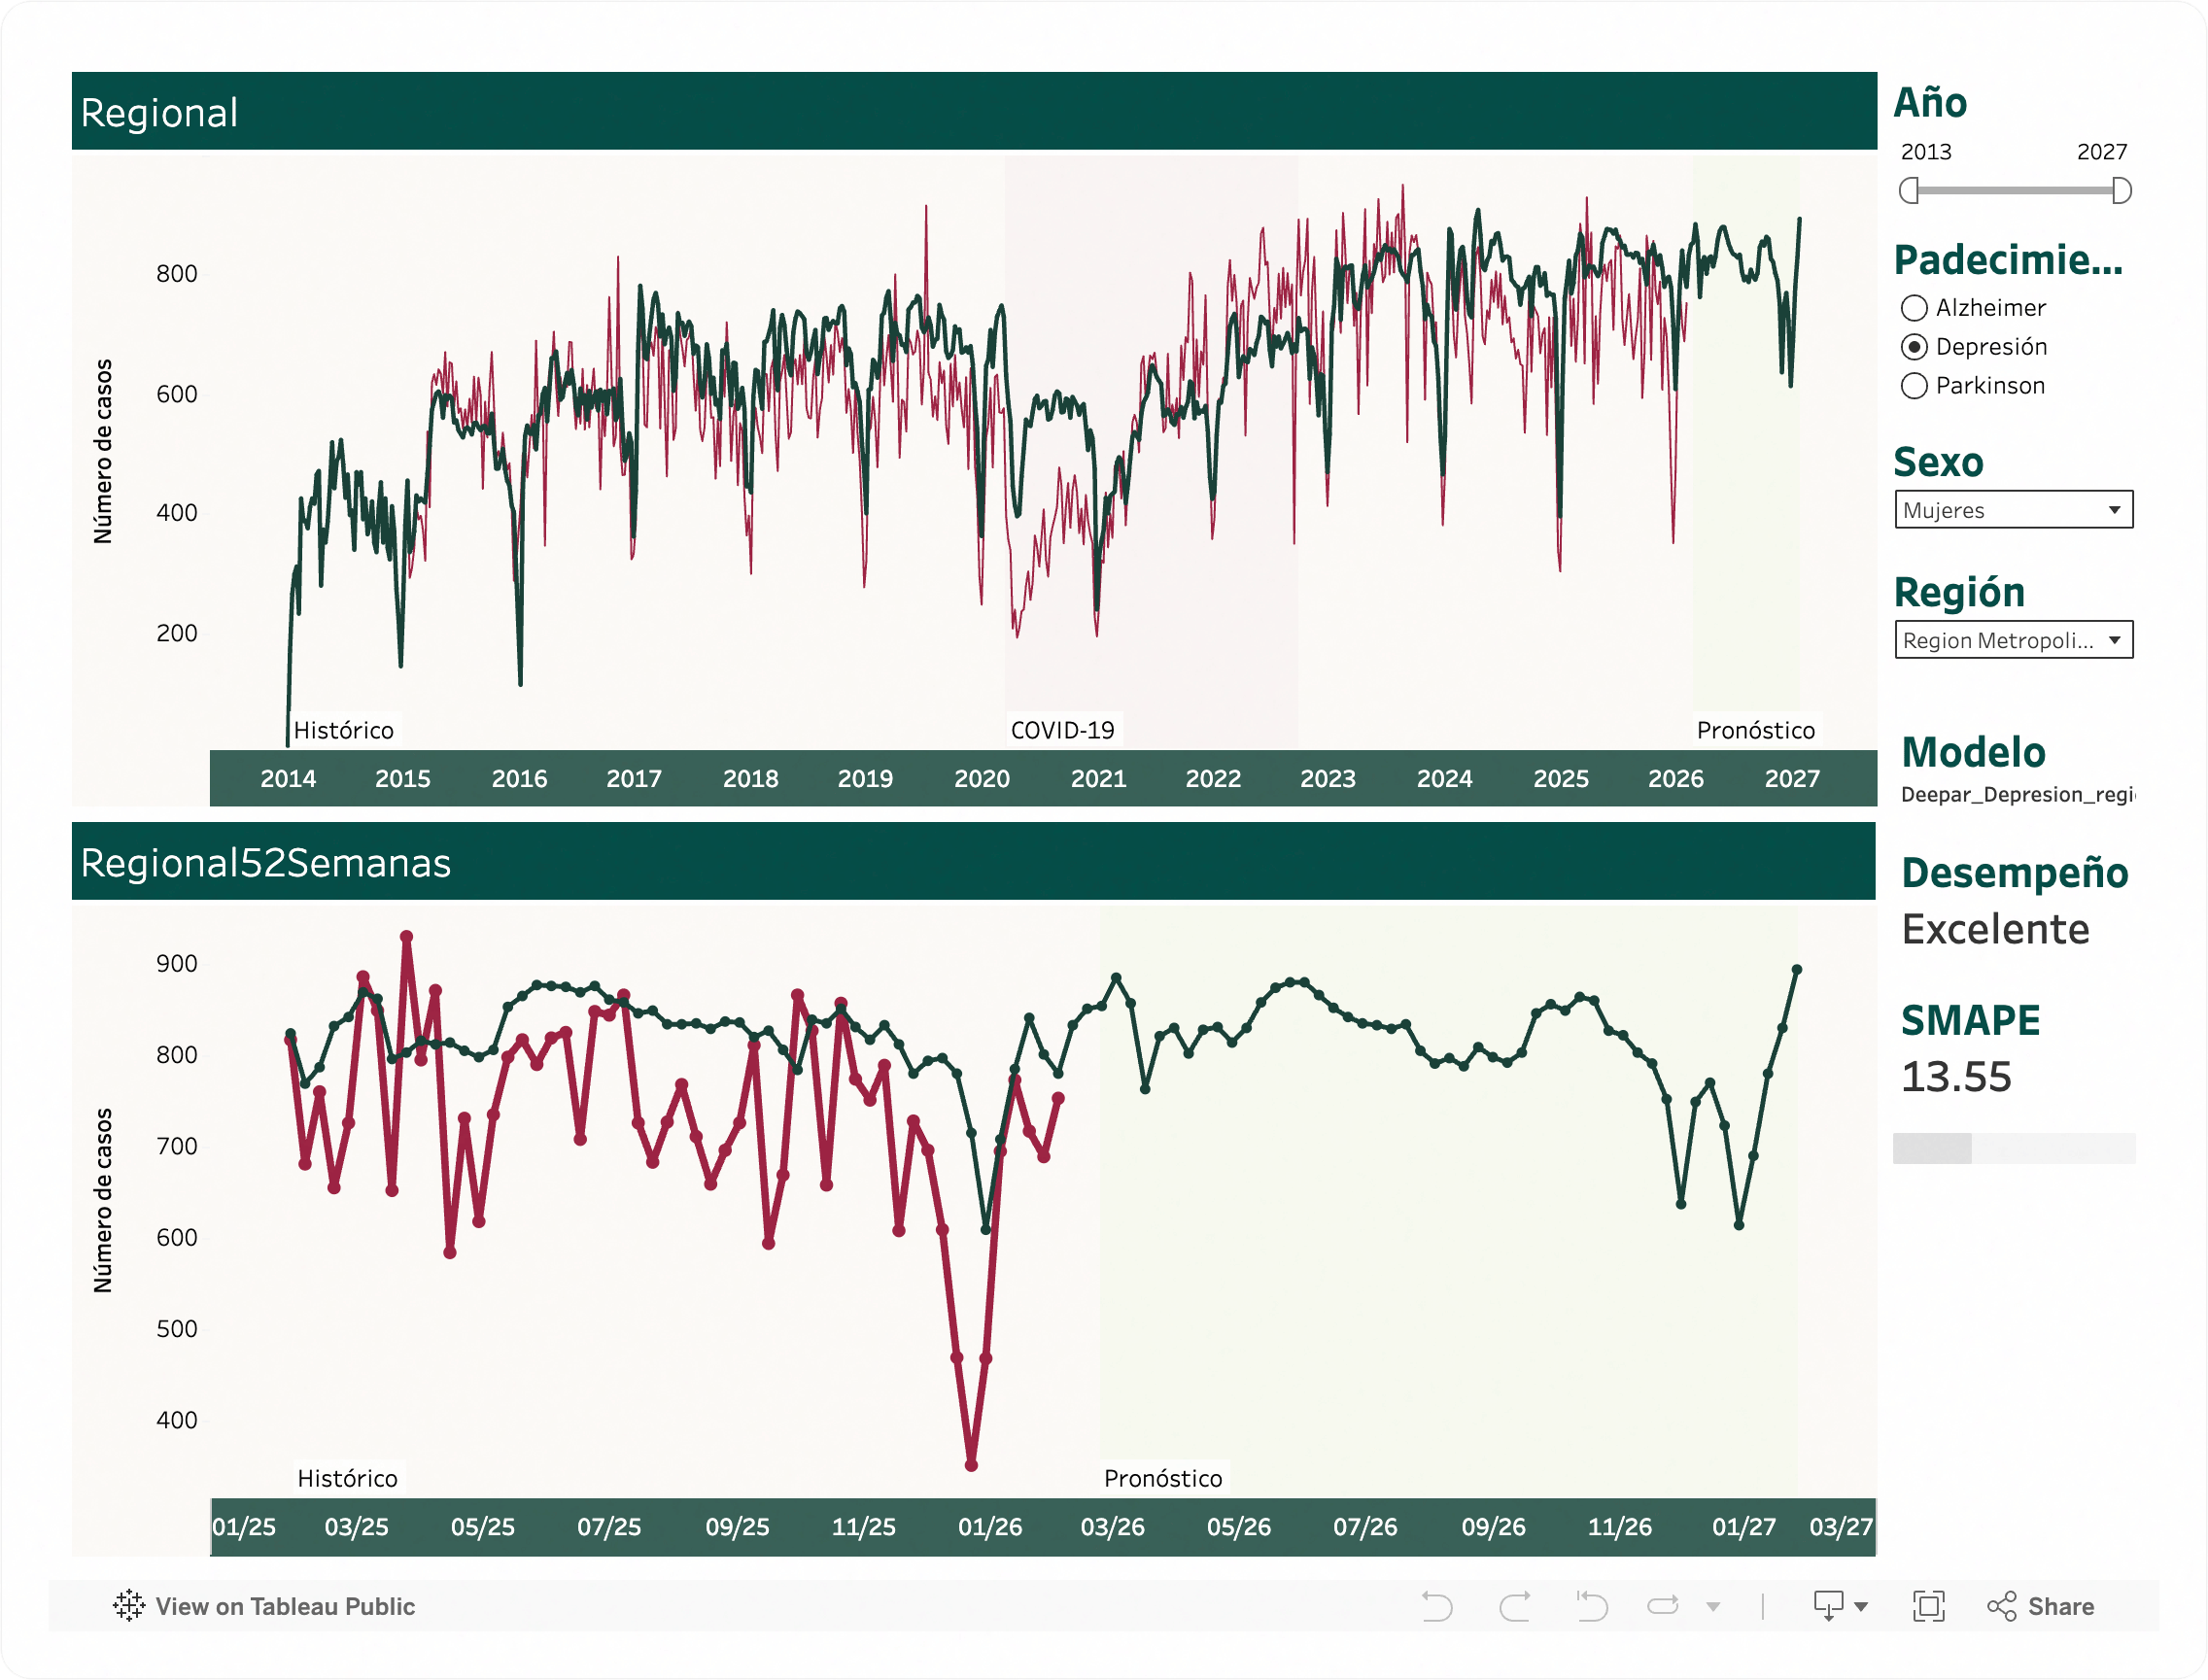
\includegraphics[width=\textwidth]{prediccion-regional.png}
\caption[Predicción regional.]{Vista \textbf{Predicción regional}: pronóstico agregado por las cuatro regiones de salud mental con comparativa interregional.}
\label{fig:web_prediccion_regional}
\end{figure}

\subsubsection{Dashboard de KPIs}

El \textbf{DashKPIs} (\figref{fig:web_dashboard_kpis}) es la vista de control ejecutivo del sistema. Presenta los 333 modelos en producción, el \smape{} mediano global (23.66\%), la cobertura del 100\%, un heatmap de métricas por padecimiento y género, un donut chart con la distribución de algoritmos activos y una grilla de calor por serie.

\begin{figure}[H]
\centering
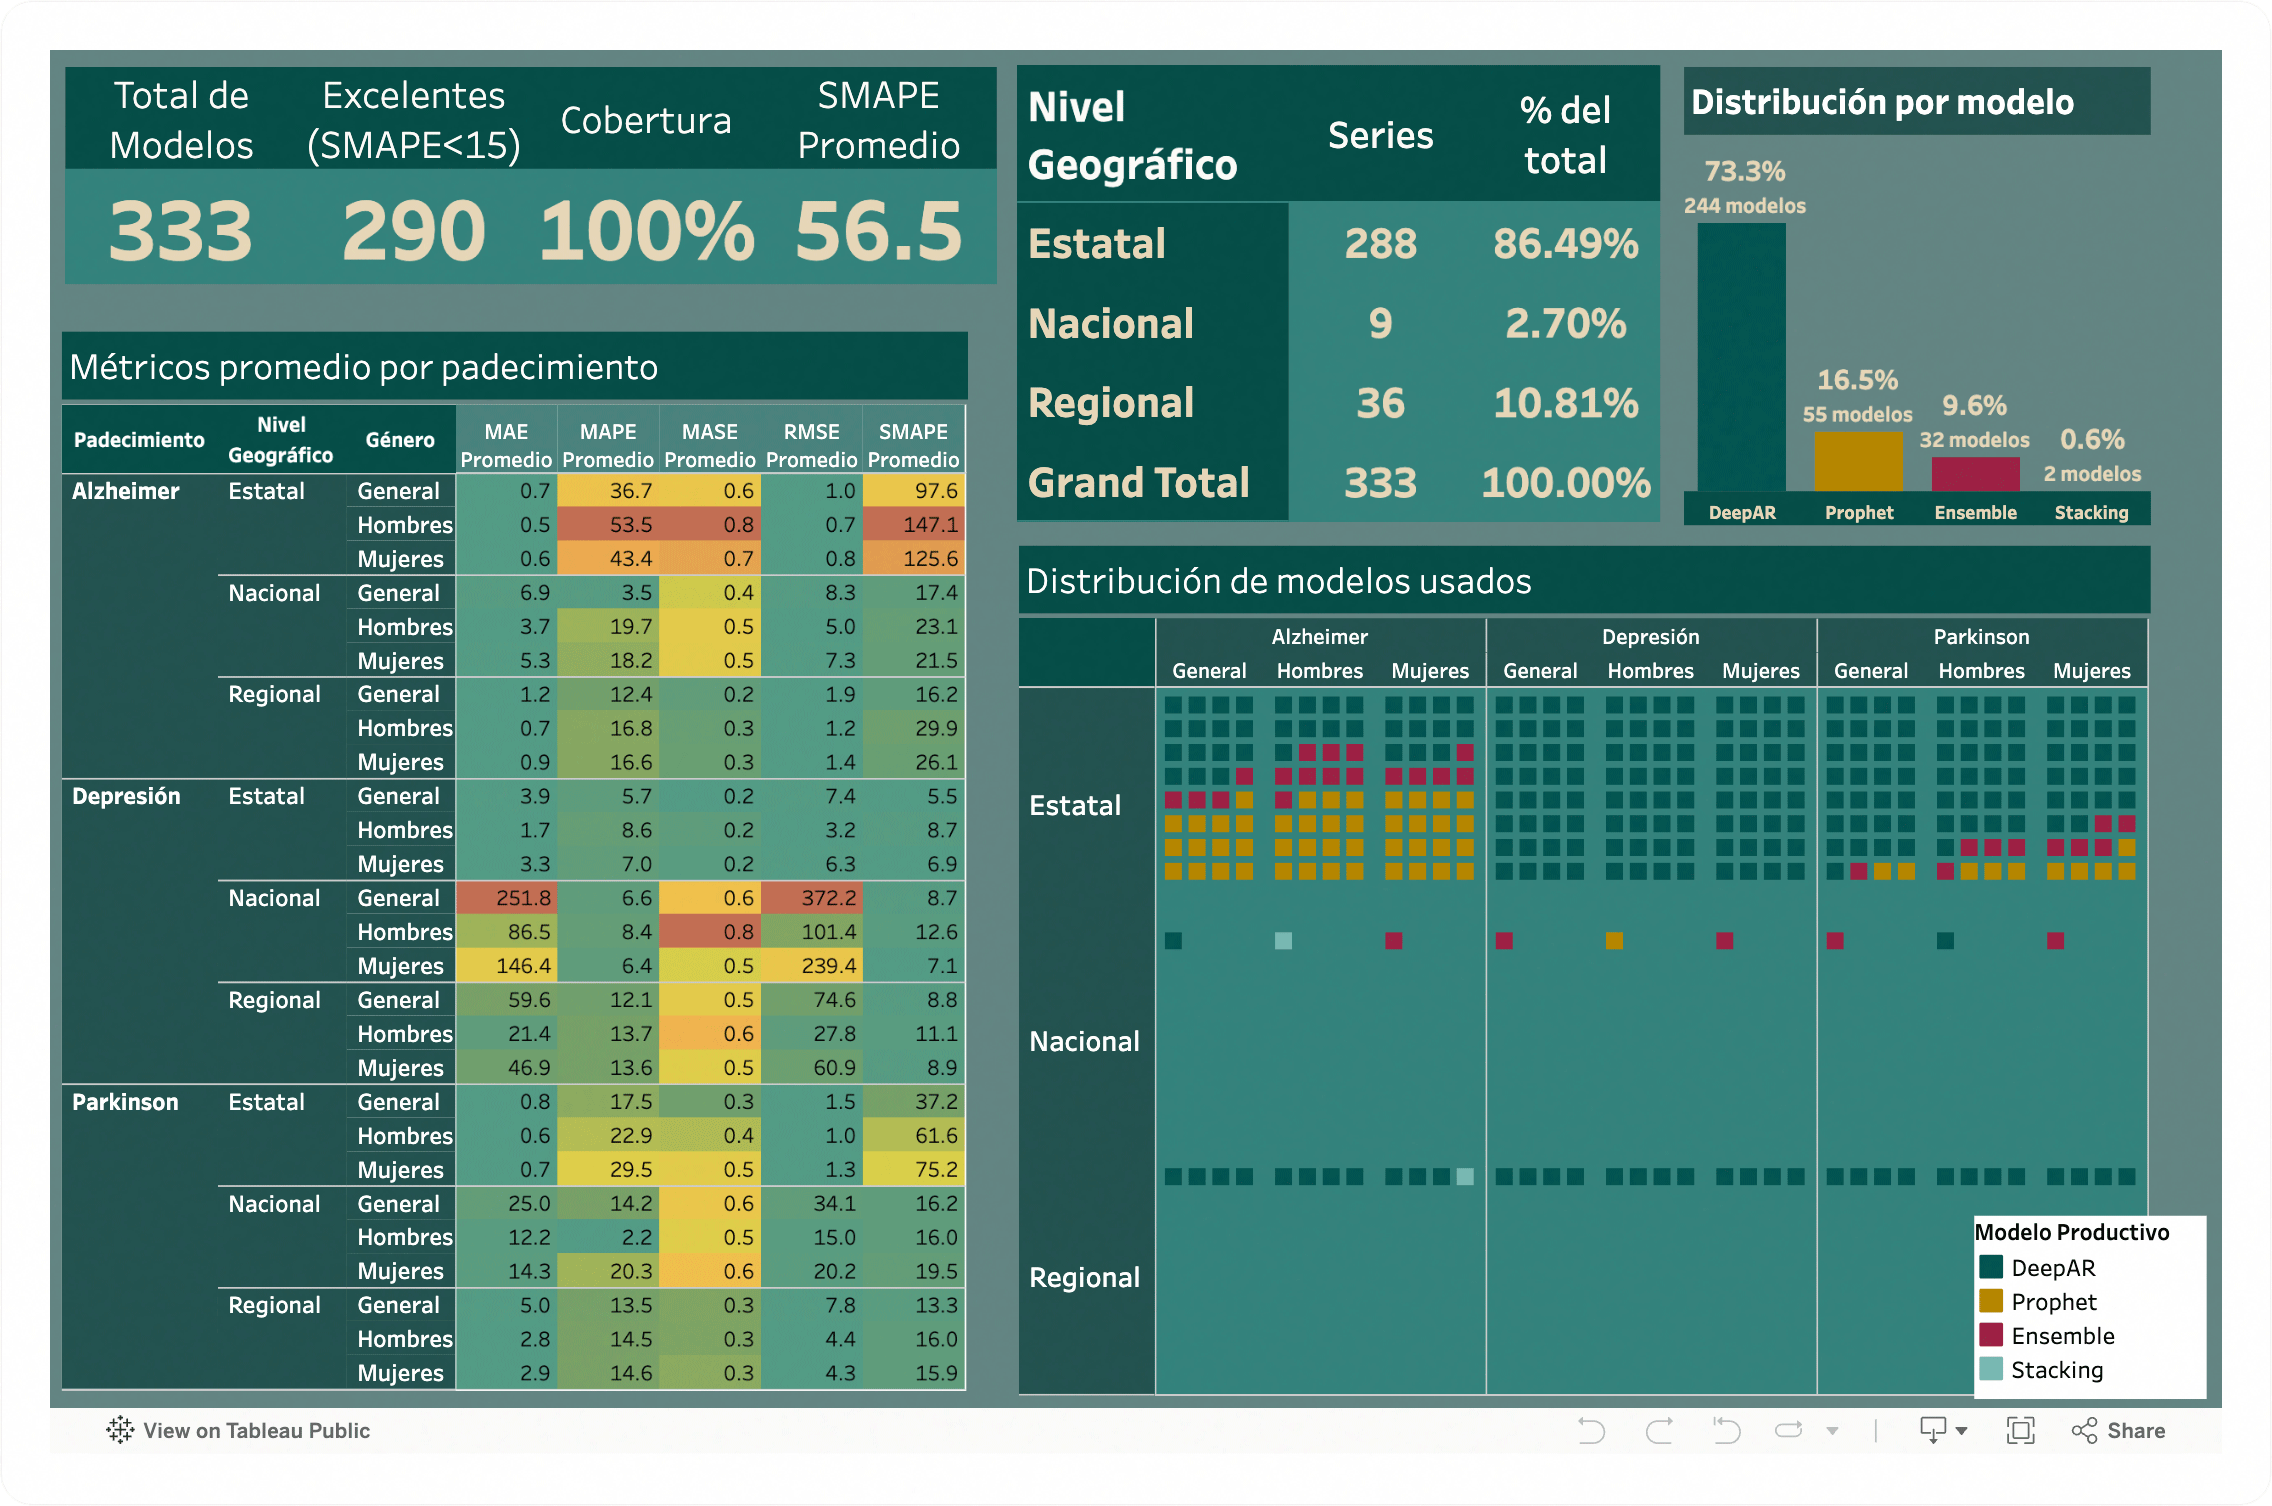
\includegraphics[width=0.85\textwidth]{dashboard-kpis}
\caption[Dashboard KPIs.]{Vista \textbf{DashKPIs}: indicadores generales del sistema, distribución de algoritmos, heatmap de métricas y mapa de calor por serie.}
\label{fig:web_dashboard_kpis}
\end{figure}

\newpage
\subsection{Integración y automatización}\label{subsec:integracion_tableau}

\subsubsection{Google Sheets como intermediario}

La razón de usar Google Sheets como intermediario (en lugar de publicar directamente desde S3) es que Tableau Public soporta actualizaciones automáticas del \textit{extract} desde Google Sheets. El script \texttt{publish\_gsheets.py} publica las cinco hojas en bloques de 5,000 filas, autenticando via cuenta de servicio GCP. Cuando se publica una nueva versión, Tableau Public refresca el extract automáticamente en $\sim$24 horas.

\subsubsection{Automatización con GitHub Actions}

El workflow \texttt{gsheets.yml} automatiza la publicación completa. Se dispara por \texttt{workflow\_call} (automático desde otro workflow) o por \texttt{workflow\_dispatch} (manual). Los secretos \texttt{GOOGLE\_SERVICE\_ACCOUNT\_JSON} y \texttt{GSHEETS\_SPREADSHEET\_ID} se inyectan como variables de entorno en el job de CI/CD.

\subsection{Decisiones técnicas de diseño}\label{subsec:decisiones_tableau}

\begin{table}[H]
\centering
\caption{Decisiones técnicas del sistema de visualización y su justificación}
\label{tab:decisiones_tableau}
\scriptsize
\setlength{\tabcolsep}{4pt}
\begin{tabularx}{\textwidth}{>{\bfseries}p{3.2cm} X X}
\toprule
\textbf{Decisión} & \textbf{Descripción} & \textbf{Justificación} \\
\midrule
Normalización por 100,000 hab. & Las vistas de evolución normalizan la incidencia por población. & Permite comparar entidades con poblaciones muy diferentes en el mismo eje. \\
\addlinespace
Recorte por percentiles & Las vistas de evolución aplican un límite superior basado en percentiles del eje Y. & Evita que outliers temporales distorsionen la escala de la gráfica. \\
\addlinespace
\texttt{scaffold} como ancla & El modelo relacional usa \texttt{scaffold} como tabla raíz. & Garantiza que los filtros se propaguen a ambas tablas de hechos. \\
\addlinespace
\texttt{yhat} entero & Los pronósticos se publican como \texttt{Int64}. & Los casos son conteos discretos; mostrar decimales carecería de significado clínico. \\
\addlinespace
Relationships, no joins & Tableau usa \textit{relationships} (modelo lógico) en lugar de \texttt{JOIN} SQL. & Evita la multiplicación de filas entre tablas con cardinalidades diferentes. \\
\bottomrule
\end{tabularx}
\end{table}

\newpage

% =============================================================================
% PROPUESTA DE DESPLIEGUE EN PRODUCCION
% =============================================================================
\section{Propuesta de Despliegue en Producción}\label{sec:despliegue}

\subsection{Arquitectura productiva}

\begin{figure}[H]
\centering
\resizebox{\textwidth}{!}{%
\begin{tikzpicture}[
    % 1. Estilo base unificado con sombras sutiles y bordes redondeados
    base/.style={
        thick, rounded corners=6pt,
        minimum width=3.4cm, minimum height=1.5cm, text width=3.2cm,
        align=center, font=\sffamily,
        drop shadow={opacity=0.12, shadow xshift=2pt, shadow yshift=-2pt}
    },
    % 2. Mantenemos tus colores clave intactos
    block/.style={base, draw=teal, fill=lightgreen},
    aws/.style={base, draw=gold, fill=lightyellow},
    store/.style={base, draw=burgundy, fill=lightred!50},
    % 3. Estilo de flechas moderno y refinado
    arrow/.style={
        -{Stealth[round, length=8pt, width=6pt]},
        thick, color=coolgray,
        shorten >=1.5pt, shorten <=1.5pt
    },
    % 4. Estilo de etiquetas tipo "badge" (píldora) con fondo blanco
    label/.style={
        font=\sffamily\scriptsize\bfseries\color{coolgray},
        fill=white, inner sep=3pt, rounded corners=4pt
    }
]
    % --- FILA 1 ---
    \node[block] (cron) at (0, 0) {\textbf{Cron / Airflow}\\[1mm]\scriptsize Semanal + Trimestral};
    \node[block] (etl) at (6, 0) {\textbf{ETL Pipeline}\\[1mm]\scriptsize (EC2 / Lambda)};
    \node[store] (s3) at (12, 0) {\textbf{S3 Bucket}\\[1mm]\scriptsize datos + modelos};

    \draw[arrow] (cron) -- node[label] {trigger} (etl);
    \draw[arrow] (etl) -- node[label] {processed/} (s3);

    % --- FILA 2 ---
    \node[aws] (sm) at (12, -3.8) {\textbf{SageMaker}\\[1mm]\scriptsize Training Job};
    \node[aws] (models) at (6, -3.8) {\textbf{Inference}\\[1mm]\scriptsize (Batch)};
    \node[block] (dash) at (0, -3.8) {\textbf{Dashboard}\\[1mm]\scriptsize Tableau / Web};

    \draw[arrow] (s3) -- node[label] {input} (sm);
    \draw[arrow] (sm) -- node[label] {modelos .pkl} (models);
    \draw[arrow] (models) -- node[label] {forecasts} (dash);

    % --- FILA 3 ---
    \node[aws] (monitor) at (6, -7.6) {\textbf{CloudWatch}\\[1mm]\scriptsize Monitoreo};
    \node[block] (alert) at (12, -7.6) {\textbf{SNS Alertas}\\[1mm]\scriptsize (email / Slack)};

    \draw[arrow] (sm) -- (monitor);
    \draw[arrow] (models) -- (monitor);
    \draw[arrow] (monitor) -- node[label] {drift} (alert);

\end{tikzpicture}
}% fin resizebox
\caption[Arquitectura productiva en AWS.]{Arquitectura productiva propuesta para EpiForecast-MX en AWS}
\label{fig:arquitectura_prod}
\end{figure}
\subsection{Estrategia de reentrenamiento trimestral}

Se recomienda un ciclo de reentrenamiento \textbf{trimestral} en lugar de semanal, por las siguientes razones:

\begin{enumerate}[noitemsep]
    \item \textbf{Estabilidad de las series}: los tres padecimientos modelados (Depresión, Parkinson, Alzheimer) presentan dinámicas de cambio lento: la estacionalidad es anual, las tendencias se mueven en escala de meses o años, y los patrones demográficos subyacentes (envejecimiento, urbanización) operan en horizontes de décadas. Un modelo entrenado con datos hasta la semana $t$ no se degrada significativamente en 13 semanas.
    \item \textbf{Horizonte de pronóstico de 52 semanas}: el sistema genera pronósticos a un año completo. Reentrenar semanalmente produciría 52 modelos anuales donde cada uno difiere del anterior en apenas $\approx$0.17\% de los datos de entrenamiento (1 semana nueva sobre $\approx$600 semanas históricas), generando variación innecesaria en los pronósticos sin mejorar la precisión.
    \item \textbf{Costo-beneficio}: el entrenamiento completo de 333 modelos en SageMaker cuesta \$3.50\,--\,\$8.50 USD por job de entrenamiento. Con reentrenamiento semanal el costo anual sería \$182\,--\,\$442 USD solo en entrenamiento; con reentrenamiento trimestral se reduce a \$14\,--\,\$34 USD anuales, un ahorro del 92\% sin degradación significativa esperada en la precisión, dado que cada semana adicional representa aproximadamente 1 observación sobre un historial del orden de 600 semanas ($\approx$0.17\%).
    \item \textbf{Validación rigurosa}: cada reentrenamiento requiere validación humana (revisión de métricas, diagnóstico de overfitting, aprobación del epidemiólogo). Un ciclo semanal saturaría al equipo con tareas repetitivas de bajo valor; un ciclo trimestral permite dedicar tiempo real a la revisión de calidad.
    \item \textbf{Consistencia para stakeholders}: los tomadores de decisiones del {\imss} planifican en ciclos trimestrales (solicitudes de medicamentos, presupuestos delegacionales). Un pronóstico que cambia cada semana genera confusión; un pronóstico estable por trimestre se integra naturalmente al flujo institucional.
\end{enumerate}

\begin{warningbox}[¿Cuándo sí reentrenar antes del trimestre?]
El reentrenamiento anticipado se activa automáticamente si se detecta \textbf{drift significativo}: cuando el \smape{} acumulado de las últimas 4 semanas supera 1.5$\times$ el \smape{} de validación cruzada, o cuando un evento exógeno (pandemia, cambio de política sanitaria, desastre natural) altera la dinámica epidemiológica. El monitoreo semanal de métricas se mantiene activo para detectar estas situaciones.
\end{warningbox}

\subsubsection{Calendario de operaciones}

El sistema opera en dos ciclos diferenciados: un ciclo \textbf{semanal} ligero (solo inferencia y monitoreo) y un ciclo \textbf{trimestral} pesado (reentrenamiento completo), cuya secuencia visual se presenta en la \figref{fig:calendario_ops} y cuyo detalle técnico se desglosa en la \tabref{tab:calendario}.

\begin{figure}[H]
\centering
\makebox[\textwidth][c]{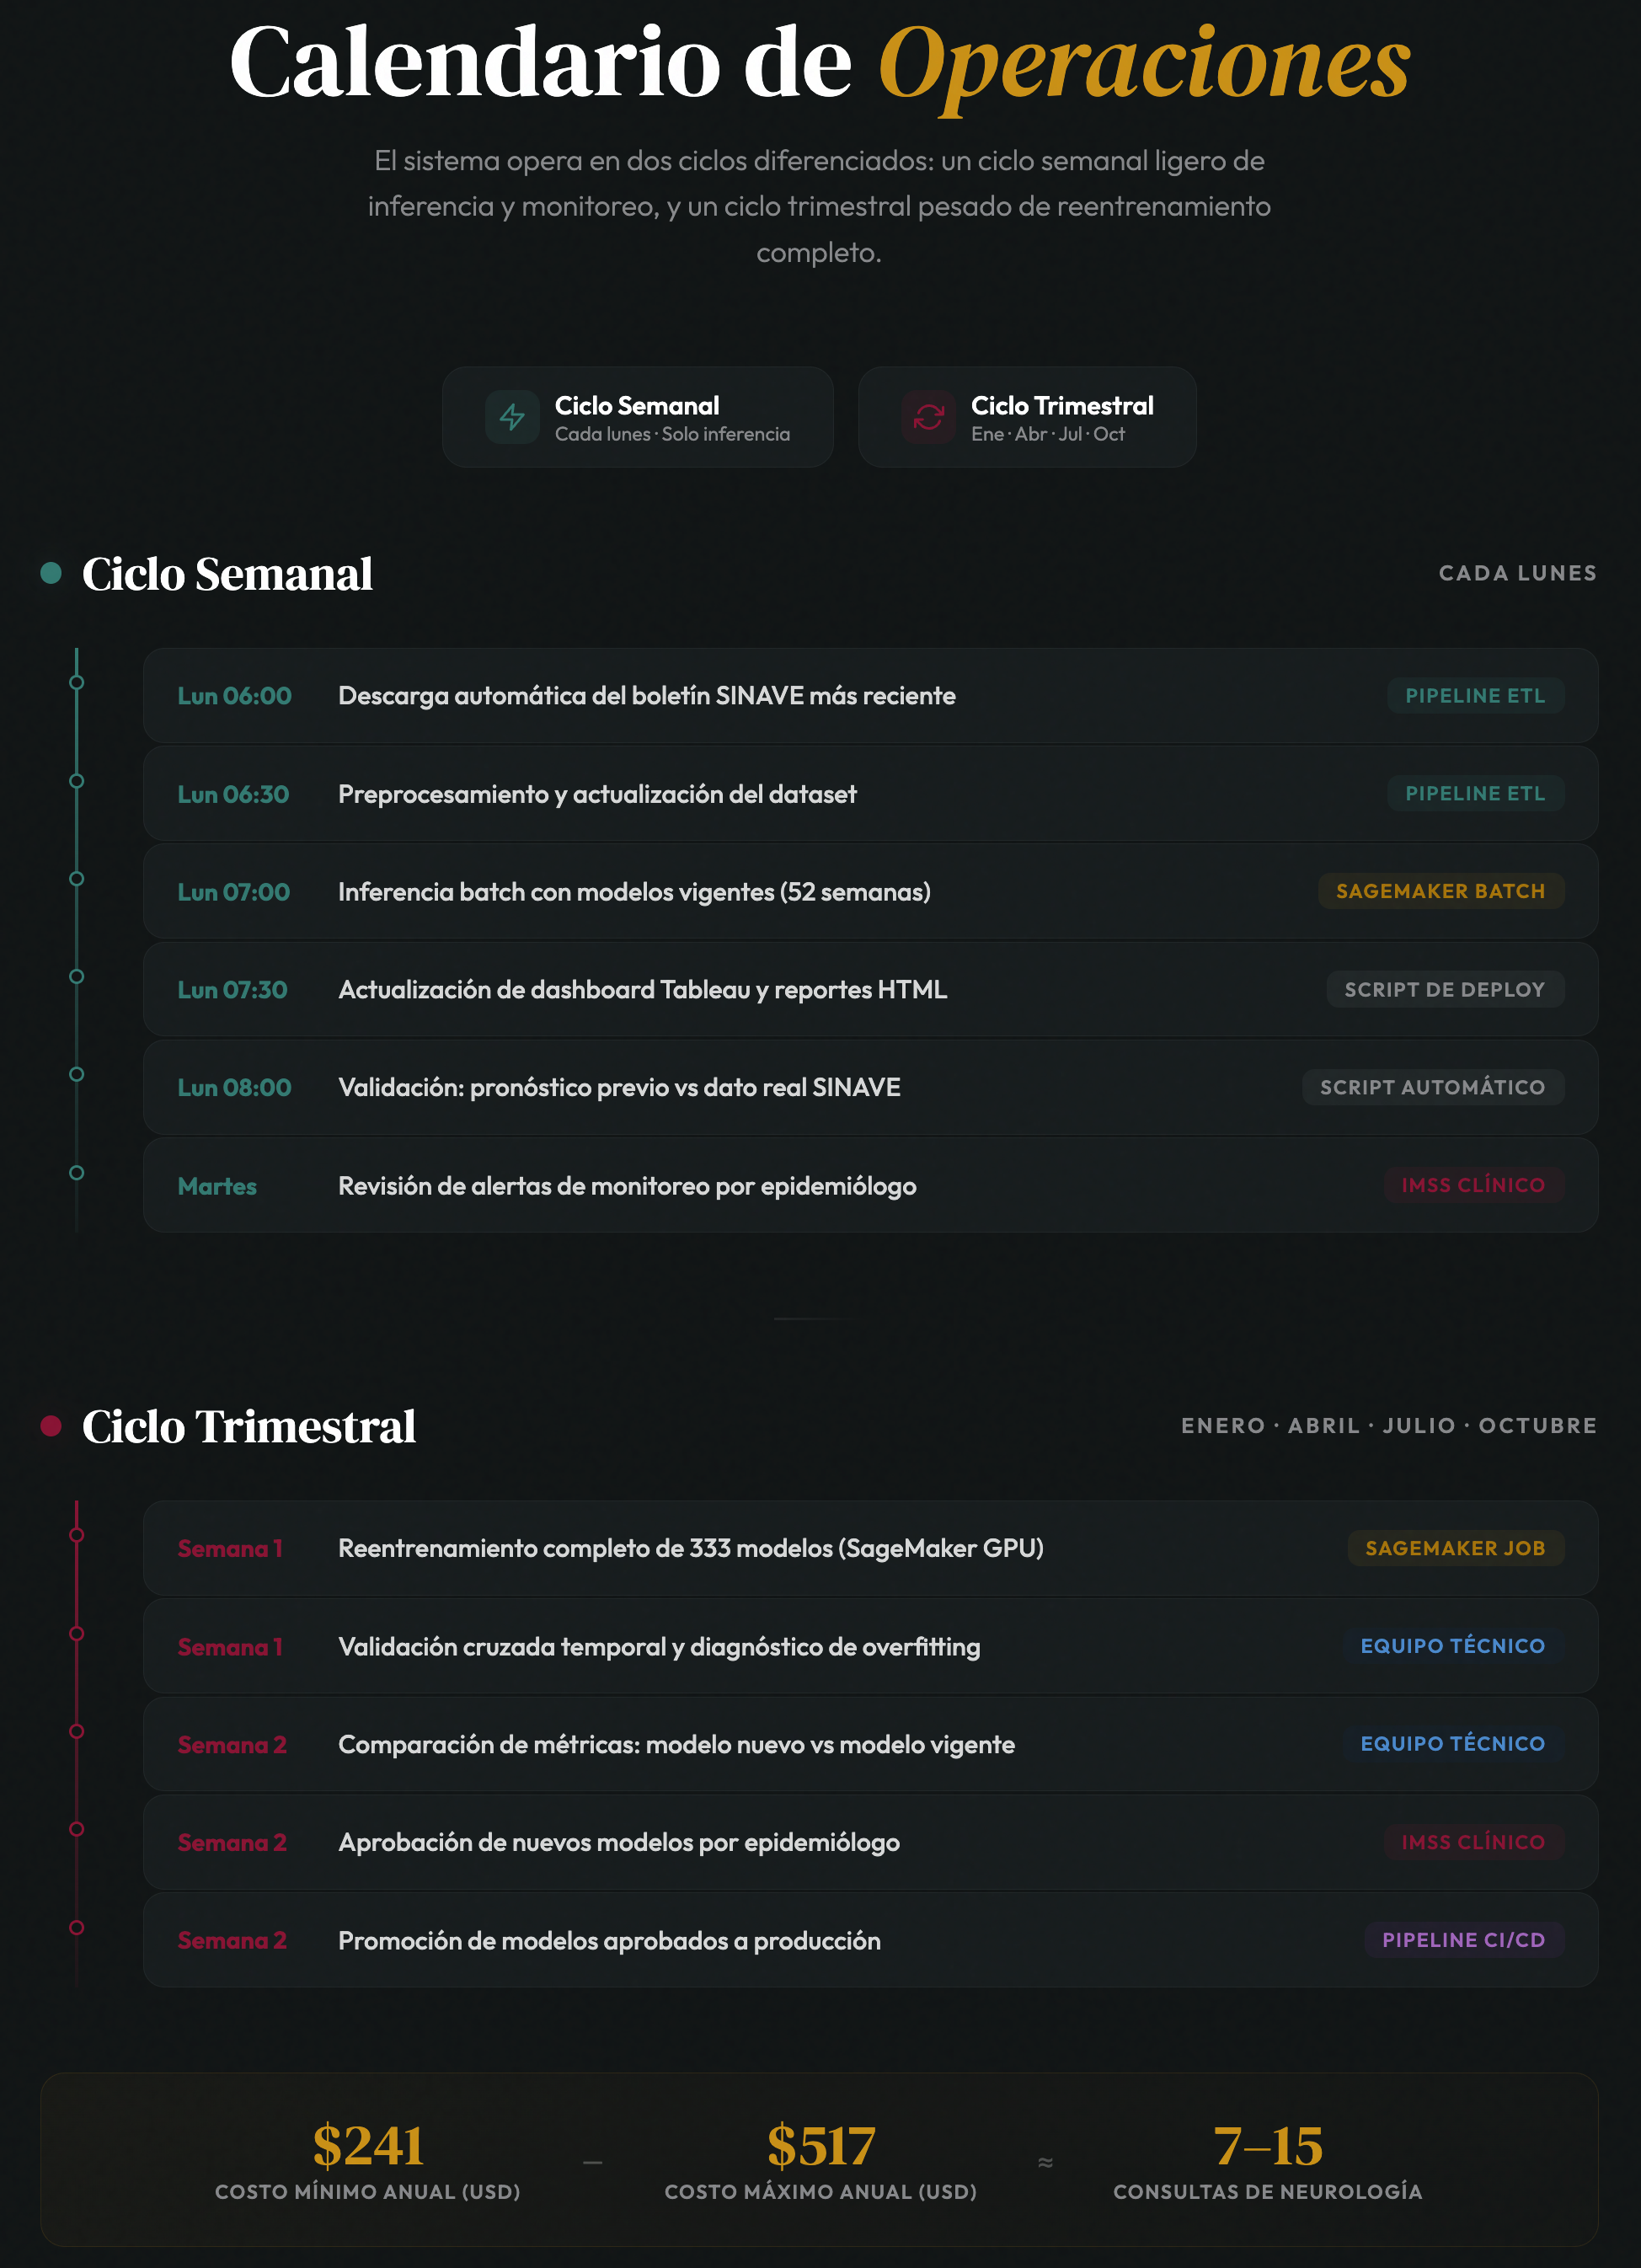
\includegraphics[width=0.9\textwidth]{PropuestaDeployments.png}}
\caption[Calendario de operaciones.]{Calendario de operaciones de EpiForecast-MX: ciclo semanal (inferencia cada lunes) y ciclo trimestral (reentrenamiento completo en enero, abril, julio y octubre). El costo operativo anual es de \$240\,--\,\$506 USD.}
\label{fig:calendario_ops}
\end{figure}

\begin{table}[H]
\centering
\caption{Calendario de operaciones: ciclo semanal (inferencia) y ciclo trimestral (reentrenamiento)}
\label{tab:calendario}
\small
\begin{tabularx}{\textwidth}{l l X l}
\toprule
\textbf{Ciclo} & \textbf{Día} & \textbf{Actividad} & \textbf{Responsable} \\
\midrule
\multicolumn{4}{l}{\textit{Ciclo semanal (cada lunes, solo inferencia)}} \\
\midrule
Semanal & Lunes 06:00 & Descarga automática del boletín SINAVE más reciente & Pipeline ETL \\
Semanal & Lunes 06:30 & Preprocesamiento y actualización del dataset & Pipeline ETL \\
Semanal & Lunes 07:00 & Inferencia batch con modelos vigentes (52 semanas) & SageMaker Batch \\
Semanal & Lunes 07:30 & Actualización de dashboard Tableau y reportes HTML & Script de deploy \\
Semanal & Lunes 08:00 & Validación: pronóstico previo vs dato real SINAVE & Script automático \\
Semanal & Martes & Revisión de alertas de monitoreo por epidemiólogo & IMSS Clínico \\
\midrule
\multicolumn{4}{l}{\textit{Ciclo trimestral (enero, abril, julio, octubre)}} \\
\midrule
Trimestral & Semana 1 & Reentrenamiento completo de 333 modelos (SageMaker GPU) & SageMaker Job \\
Trimestral & Semana 1 & Validación cruzada temporal y diagnóstico de overfitting & Equipo Técnico \\
Trimestral & Semana 2 & Comparación de métricas: modelo nuevo vs modelo vigente & Equipo Técnico \\
Trimestral & Semana 2 & Aprobación de nuevos modelos por epidemiólogo & IMSS Clínico \\
Trimestral & Semana 2 & Promoción de modelos aprobados a producción & Pipeline CI/CD \\
\bottomrule
\end{tabularx}
\end{table}

\subsection{Estrategia de monitoreo}

El monitoreo opera \textbf{semanalmente} (aunque el reentrenamiento sea trimestral) y se basa en tres pilares, cuya estructura se visualiza en la \figref{fig:estrategia_monitoreo}:

\begin{figure}[H]
\centering
\makebox[\textwidth][c]{
\includegraphics[width=1.15\textwidth]{estrategia_monitoreo.png}}
\caption[Estrategia de monitoreo.]{Los tres pilares del monitoreo semanal: drift de datos (Kolmogorov-Smirnov), degradación de métricas (\smape{} vs CV) y anomalías operativas (CloudWatch Alarms), con sus umbrales de activación y flujo de respuesta.}
\label{fig:estrategia_monitoreo}
\end{figure}

\begin{enumerate}[noitemsep]
    \item \textbf{Drift de datos}: cada lunes, comparar la distribución de nuevos boletines SINAVE contra la distribución histórica. Si el test de Kolmogorov-Smirnov detecta desviación significativa ($p < 0.05$) durante 4 semanas consecutivas, activar reentrenamiento anticipado.
    \item \textbf{Degradación de métricas}: monitorear el \smape{} semanal acumulado por serie. Si supera 1.5$\times$ el \smape{} de CV en más del 10\% de las series, activar reentrenamiento fuera de ciclo trimestral.
    \item \textbf{Anomalías operativas}: CloudWatch Alarms para fallos de SageMaker, tiempos de ejecución anormales ($>$2$\times$ promedio) y errores de S3.
\end{enumerate}

\subsection{Proyección de costos a 12 meses}

La \figref{fig:costos_aws} presenta el desglose visual de costos anuales por componente AWS, incluyendo la comparativa de ahorro entre reentrenamiento trimestral y semanal.

\begin{figure}[H]
\centering
\makebox[\textwidth][c]{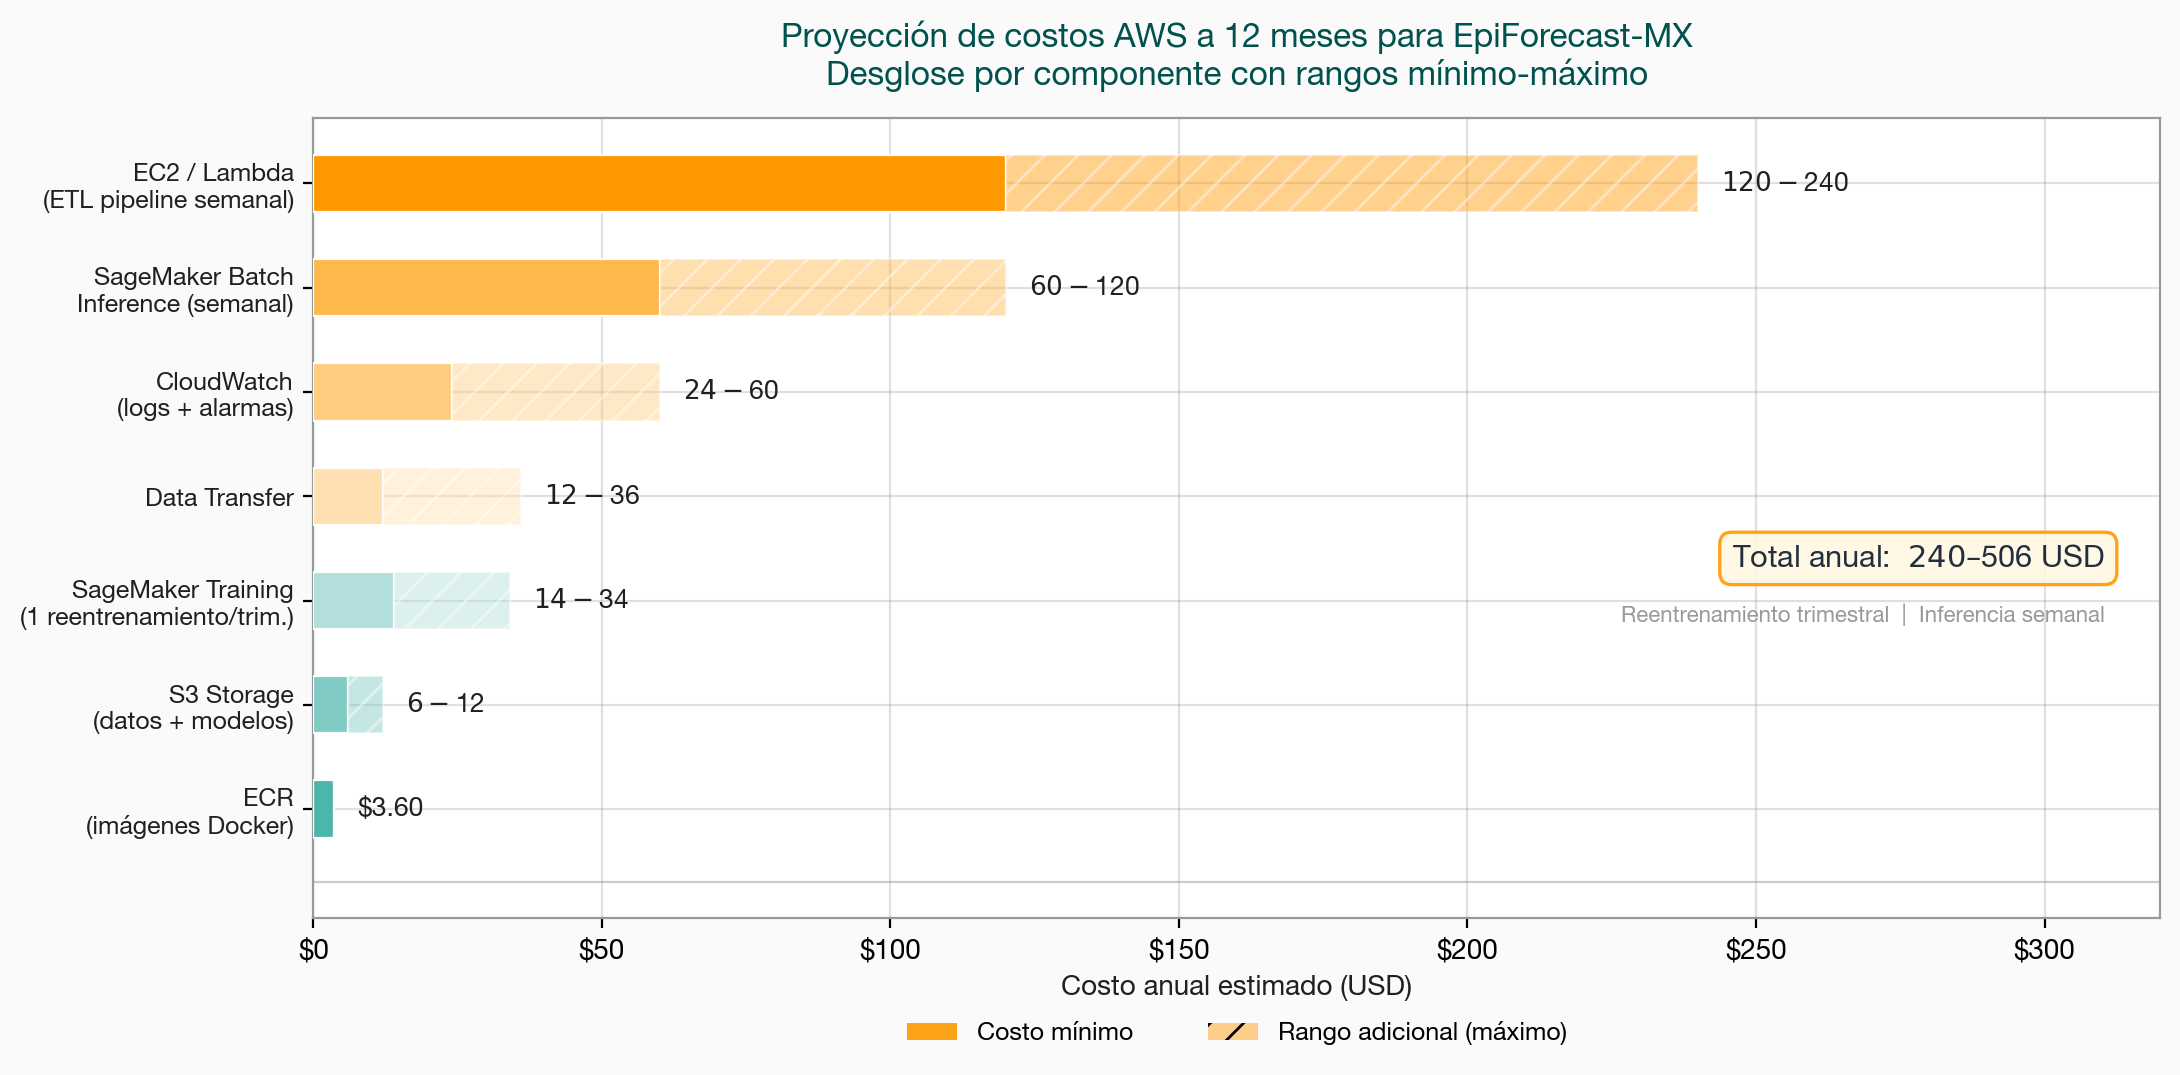
\includegraphics[width=1.15\textwidth]{fig_costos_aws_12m.png}}
\caption[Proyección de costos AWS a 12 meses.]{Desglose de costos anuales por componente AWS con reentrenamiento trimestral (\$240\,--\,\$506 USD). El esquema trimestral representa un ahorro de más del 40\% respecto al semanal.}
\label{fig:costos_aws}
\end{figure}

\begin{table}[H]
\centering
\caption{Proyección de costos AWS a 12 meses (reentrenamiento trimestral)}
\label{tab:costos_12m}
\scriptsize
\begin{tabularx}{\textwidth}{X r r}
\toprule
\textbf{Componente} & \textbf{\shortstack[r]{Costo trimestral\\(USD)}} & \textbf{\shortstack[r]{Costo anual\\(USD)}} \\
\midrule
SageMaker Training (1 reentrenamiento/trimestre)  & \$3.50\,--\,8.50  & \$14\,--\,34 \\
SageMaker Batch Inference (semanal)               & \$15\,--\,30       & \$60\,--\,120 \\
S3 Storage (datos + modelos)                      & \$1.50\,--\,3.00   & \$6\,--\,12 \\
ECR (imágenes Docker)                             & \$0.90             & \$3.60 \\
CloudWatch (logs + alarmas semanales)              & \$6\,--\,15        & \$24\,--\,60 \\
EC2/Lambda (ETL pipeline semanal)                  & \$30\,--\,60       & \$120\,--\,240 \\
Data Transfer                                     & \$3\,--\,9         & \$12\,--\,36 \\
\midrule
\textbf{Total estimado (USD)}                           & \textbf{\$60\,--\,127} & \textbf{\$240\,--\,506} \\
\bottomrule
\end{tabularx}
\end{table}

\begin{insightbox}[Costo-beneficio: más del 40\% de ahorro en costo operativo total]
Con reentrenamiento trimestral, el costo anual se reduce a \textbf{\$240\,--\,\$506 USD}, un ahorro de más del 40\% respecto al esquema semanal original (\$408\,--\,\$914 USD). El ahorro de 92\% corresponde únicamente al componente de entrenamiento GPU (de 52 a 4 jobs anuales); el ahorro operativo total es de más del 40\% porque los costos de inferencia, ETL, almacenamiento y monitoreo permanecen activos semanalmente. Para una institución del tamaño del {\imss}, este costo es marginal (véase la equivalencia en consultas de neurología en la p.~\pageref{sec:resumen}).
\end{insightbox}

\newpage
% =============================================================================
% 11. TRABAJO FUTURO
% =============================================================================
\section{Trabajo Futuro}\label{sec:futuro}

\subsection{Desagregación por rango de edad}

Actualmente el sistema desagrega por sexo (Combinado, Masculino, Femenino). Una mejora natural es agregar rangos de edad (pediátrico, adulto joven, adulto mayor), lo que multiplicaría las series de producción pero aportaría granularidad clínica valiosa para la planificación de recursos especializados.

\subsection{Integración de datos de mortalidad}

El Subsistema Epidemiológico y Estadístico de Defunciones (SEED) del {\imss} registra la mortalidad por causa. Integrar estos datos permitiría modelar no solo la incidencia sino también la letalidad, generando un indicador compuesto de carga de enfermedad.

\subsection{Análisis farmacológico}

Cruzar los pronósticos de incidencia con datos de consumo farmacéutico (recetas surtidas en farmacias IMSS) permitiría:
\begin{itemize}[noitemsep]
    \item Detectar brechas entre incidencia pronosticada y medicamentos disponibles.
    \item Optimizar la cadena de suministro de antidepresivos, levodopa y memantina.
    \item Modelar la demanda farmacéutica con los mismos motores de pronóstico.
\end{itemize}

\subsection{Expansión a condiciones adicionales}

El framework modular (patrón Factory) permite agregar nuevos padecimientos sin modificar el código existente:
\begin{itemize}[noitemsep]
    \item \textbf{Diabetes mellitus (E11)}: alta incidencia, impacto presupuestal crítico.
    \item \textbf{Hipertensión arterial (I10)}: primera causa de consulta en primer nivel.
    \item \textbf{Ansiedad (F41)}: complemento natural de Depresión.
    \item \textbf{Epilepsia (G40)}: padecimiento neurológico con patrones estacionales.
\end{itemize}

\subsection{Publicaciones académicas}

En colaboración con el {\imss}, se trabaja activamente en la preparación de un artículo científico enfocado en la metodología del proyecto, con el título provisional:

\begin{quote}
\textit{``A Methodological Framework for Artificial Intelligence–Based Predictive Modelling in Digital Health''}
\end{quote}

Este artículo, orientado al eje ``de los datos a la predicción'', documenta el marco metodológico para la salud digital basado en inteligencia artificial, con aplicaciones clínicas concretas derivadas de EpiForecast-MX. Se tiene como objetivo someter dicho artículo a foros y revistas especializadas en enfermedades mentales y vigilancia epidemiológica.

Adicionalmente, se contempla un segundo artículo futuro centrado en los \textbf{resultados cuantitativos} del proyecto: el desempeño comparativo de los cuatro motores de pronóstico sobre las 333 series de producción, las lecciones aprendidas del despliegue en AWS SageMaker y las implicaciones clínicas de los pronósticos para el {\imss}. La plataforma de difusión de estos resultados es el sitio oficial del proyecto (\figref{fig:website}).

\begin{figure}[H]
\centering
\includegraphics[width=0.85\textwidth]{fig_website_proyecto.png}
\caption[Sitio web del proyecto.]{Página principal de \url{https://proyectointegrador.org}, donde se documenta la metodología, resultados y equipo de EpiForecast-MX.}
\label{fig:website}
\end{figure}

\newpage

% =============================================================================
% 12. REFLEXIONES PERSONALES DEL EQUIPO
% =============================================================================
\section{Reflexiones Personales del Equipo}\label{sec:reflexiones}

\subsection{Javier A. Rebull Saucedo}

\begin{wrapfigure}{r}{3cm}
\vspace{-0.5cm}

\includegraphics[width=3cm]{JARS2026.jpg}
\vspace{-1cm}
\end{wrapfigure}

EpiForecast-MX representó un desafío integral que unió mis dos mundos: la ingeniería de software y la inteligencia artificial. Diseñar un sistema que pasara de boletines PDF a pronósticos de 52 semanas con 333 modelos en producción me obligó a aplicar principios SOLID, Clean Code y MLOps a un nivel que ningún curso aislado me habría exigido. La experiencia de entrenar DeepAR en AWS SageMaker, manejar contenerización Docker, CI/CD con GitHub Actions y versionado con DVC consolidó habilidades que ya llevo a mi trabajo diario en Santander.

Lo más valioso fue el impacto real: saber que estos modelos pueden ayudar al IMSS a planificar mejor la atención de salud mental para millones de mexicanos le da un propósito profundo al esfuerzo técnico. Trabajar junto a Juan Carlos (con su visión institucional desde el IMSS) y Luis (con su rigor de ingeniería de Tesla) me enseñó que los mejores proyectos nacen cuando las disciplinas convergen. Me llevo de esta maestría no solo habilidades técnicas, sino la certeza de que la IA puede transformar la salud pública cuando se construye con rigor, ética y datos reales.

\subsection{Juan Carlos Pérez Nava}

\begin{wrapfigure}{r}{3cm}
\vspace{-0.5cm}

\includegraphics[width=3cm]{JARCOS2026.jpg}
\vspace{-1cm}
\end{wrapfigure}

Como servidor público del IMSS, este proyecto tuvo un significado especial: representó la oportunidad de aplicar inteligencia artificial directamente al sistema de salud donde trabajo. Conocer de primera mano los retos de la vigilancia epidemiológica me permitió aportar una perspectiva institucional al equipo, asegurando que el diseño técnico respondiera a necesidades reales de los epidemiólogos y tomadores de decisiones del Instituto.

Durante el desarrollo aprendí a navegar entre dos lenguajes: el de los datos y el de la gestión pública. Comprender los motores de pronóstico, las métricas de evaluación y la infraestructura cloud fue un crecimiento profesional enorme, pero lo que más me enorgullece es haber tendido el puente entre el equipo técnico y los stakeholders del IMSS. EpiForecast-MX demuestra que la transformación digital en el sector salud es posible con equipos interdisciplinarios. Llevaré conmigo la convicción de que la IA no reemplaza al criterio clínico, sino que lo potencia con evidencia cuantitativa para tomar mejores decisiones.

\newpage

\subsection{Luis G. Sánchez Salazar}

\begin{wrapfigure}{r}{3cm}
\vspace{-0.5cm}

\includegraphics[width=3cm]{LUIS2026.jpg}
\vspace{-1cm}
\end{wrapfigure}

Mi formación como ingeniero de controles en Tesla me enseñó a diseñar sistemas robustos, pero EpiForecast-MX me retó a aplicar esa mentalidad en un dominio completamente diferente: la epidemiología. Pasar de señales industriales a series de tiempo de salud mental me permitió descubrir paralelismos fascinantes entre el control de procesos y el pronóstico epidemiológico: ambos requieren detección de anomalías, manejo de ruido y retroalimentación continua.

Mi contribución abarcó dos frentes complementarios. Por un lado, me encargué de construir el Dashboard Tableau que consume los resultados de los 333 modelos de producción: diseñé las tres vistas (tablero general, predicción con zoom temporal y casos acumulados por año), automaticé la ingesta de datos desde el pipeline hacia Tableau y configuré los filtros interactivos que permiten a los epidemiólogos del {\imss} explorar cualquier combinación de padecimiento, entidad y sexo sin conocimiento técnico. Por otro lado, aporté a la infraestructura de calidad del proyecto: 855 pruebas automatizadas, cobertura de código del 92\% y un pipeline de CI/CD funcional que garantiza la confiabilidad que exige un sistema destinado al sector salud. Trabajar con Javier y Juan Carlos me demostró el valor de la diversidad profesional: cada uno aportó desde su trinchera para construir algo que ninguno habría logrado solo. Me llevo la convicción de que un buen dashboard es tan importante como el mejor algoritmo, porque un modelo que nadie puede interpretar no transforma ninguna decisión.

% =============================================================================
% 13. REFERENCIAS (APA 7.ª edición, orden alfabético, dos columnas)
% =============================================================================
\newpage
\section{Referencias}\label{sec:referencias}

\begin{multicols}{2}
\small
\setlength{\parindent}{0pt}
\setlength{\hangafter}{1}
\setlength{\parskip}{6pt}
\everypar{\hangindent=1.27cm}

Amazon Web Services. (2025). \textit{Amazon SageMaker developer guide}. \url{https://docs.aws.amazon.com/sagemaker/latest/dg/}

Chen, T., \& Guestrin, C. (2016). XGBoost: A scalable tree boosting system. En \textit{Proceedings of the 22nd ACM SIGKDD International Conference on Knowledge Discovery and Data Mining} (pp. 785--794). ACM. \url{https://doi.org/10.1145/2939672.2939785}

Google Cloud. (2025). \textit{Vertex AI documentation}. \url{https://cloud.google.com/vertex-ai/docs}

Hoerl, A. E., \& Kennard, R. W. (1970). Ridge regression: Biased estimation for nonorthogonal problems. \textit{Technometrics}, \textit{12}(1), 55--67.

Hyndman, R. J., \& Koehler, A. B. (2006). Another look at measures of forecast accuracy. \textit{International Journal of Forecasting}, \textit{22}(4), 679--688. \url{https://doi.org/10.1016/j.ijforecast.2006.03.001}

IBM. (2025). \textit{watsonx.ai documentation}. \url{https://www.ibm.com/docs/en/watsonx/saas}

Instituto Nacional de Estadística y Geografía. (2024). \textit{Proyecciones de población de México y las entidades federativas 2020--2070}. \url{https://www.inegi.org.mx/}

Ke, G., Meng, Q., Finley, T., Wang, T., Chen, W., Ma, W., Ye, Q., \& Liu, T.-Y. (2017). LightGBM: A highly efficient gradient boosting decision framework. En \textit{Advances in Neural Information Processing Systems}, \textit{30}, 3146--3154.

Korolov, M. (2022). Measuring the business impact of AI. \textit{CIO Magazine}. \url{https://www.cio.com/article/measuring-the-business-impact-of-ai/}

Microsoft Azure. (2025). \textit{Azure Machine Learning documentation}. \url{https://learn.microsoft.com/en-us/azure/machine-learning/}

Miller, K. (2022). Data-driven decision making in project management. \textit{Project Leadership and Society}, \textit{3}, 100054. \url{https://doi.org/10.1016/j.plas.2022.100054}

Organización Mundial de la Salud. (s.\,f.). \textit{Depresión} [Nota descriptiva]. Consultado el 7 de marzo de 2026, de \url{https://www.who.int/es/news-room/fact-sheets/detail/depression}

Salinas, D., Flunkert, V., Gasthaus, J., \& Januschowski, T. (2020). DeepAR: Probabilistic forecasting with autoregressive recurrent networks. \textit{International Journal of Forecasting}, \textit{36}(3), 1181--1191. \url{https://doi.org/10.1016/j.ijforecast.2019.07.001}

Secretaría de Salud. (2025). \textit{Boletines epidemiológicos del SINAVE}. Dirección General de Epidemiología. \url{https://www.gob.mx/salud/acciones-y-programas/direccion-general-de-epidemiologia-boletin-epidemiologico}

Taylor, S. J., \& Letham, B. (2018). Forecasting at scale. \textit{The American Statistician}, \textit{72}(1), 37--45. \url{https://doi.org/10.1080/00031305.2017.1380080}

\end{multicols}

% =============================================================================
% 14. GLOSARIO
% =============================================================================
\newpage
\section{Glosario}\label{sec:glosario}

\begin{longtable}{>{\bfseries}l p{11cm}}
\toprule
\textbf{Término} & \textbf{Definición} \\
\midrule
\endhead
\bottomrule
\endfoot
AutoML & Aprendizaje automático automatizado; proceso de automatizar la selección, configuración y entrenamiento de modelos de ML. \\
Batch Inference & Modo de inferencia donde se procesan múltiples registros de entrada de forma conjunta, en contraste con la inferencia en tiempo real. \\
Changepoint & Punto en una serie temporal donde la tendencia subyacente cambia de dirección o pendiente. \\
CI/CD & Integración Continua / Despliegue Continuo. Práctica de automatizar la compilación, pruebas y despliegue de software. \\
CIE-10 & Clasificación Internacional de Enfermedades, 10.ª revisión. Estándar de la OMS para codificar diagnósticos médicos. \\
CloudWatch & Servicio de monitoreo y observabilidad de AWS para recursos cloud y aplicaciones. \\
Cross-learning & Capacidad de un modelo (como DeepAR) de aprender patrones compartidos entre múltiples series de tiempo simultáneamente. \\
Cross-Validation & Técnica de evaluación que divide los datos en múltiples subconjuntos para estimar el rendimiento del modelo sin sesgo. \\
CV temporal & Variante de cross-validation para series de tiempo que respeta la causalidad: nunca se usa información futura para entrenar. \\
DeepAR & Red neuronal autoregresiva probabilística desarrollada por Amazon que aprende distribución de pronósticos a partir de múltiples series (Salinas et al., 2020). \\
Docker & Plataforma de contenerización que empaqueta aplicaciones y sus dependencias en unidades estandarizadas portátiles. \\
Drift & Desviación gradual de las propiedades estadísticas de los datos de entrada respecto a los datos de entrenamiento. \\
DVC & Data Version Control. Herramienta de versionado de datos y modelos compatible con Git, respaldada en almacenamiento remoto. \\
ECR & Elastic Container Registry. Servicio de AWS para almacenar imágenes Docker. \\
Ensemble & Técnica que combina múltiples modelos para producir predicciones más robustas que cualquier modelo individual. \\
ETS & Exponential Smoothing (Error, Trend, Seasonality). Familia de modelos clásicos de series de tiempo. \\
Factory Pattern & Patrón de diseño de software que encapsula la creación de objetos, permitiendo instanciar clases sin conocer la implementación concreta. \\
Feature Engineering & Proceso de crear variables derivadas a partir de datos crudos para mejorar el rendimiento de modelos de ML. \\
GluonTS & Biblioteca de Amazon para modelado probabilístico de series de tiempo, construida sobre PyTorch. \\
GPU & Graphics Processing Unit. Procesador especializado en operaciones matriciales masivamente paralelas, usado para entrenar redes neuronales. \\
IAM & Identity and Access Management. Servicio de AWS para gestionar permisos y acceso a recursos. \\
ICD-10 & Véase CIE-10. Versión en inglés de la clasificación internacional. \\
ISRS/IRSN & Inhibidores Selectivos de la Recaptación de Serotonina / Inhibidores de la Recaptación de Serotonina y Noradrenalina. Familias de antidepresivos. \\
Lag-52 & Modelo naive que predice el valor de hace 52 semanas (un año estacional). Usado como baseline para calcular \mase{} (Hyndman \& Koehler, 2006). \\
Leakage & Fuga de datos: situación donde información del conjunto de prueba se filtra al entrenamiento, inflando artificialmente las métricas. \\
LFPDPPP & Ley Federal de Protección de Datos Personales en Posesión de los Particulares. Legislación mexicana de privacidad de datos. \\
LightGBM & Gradient Boosting de Microsoft optimizado para velocidad y uso de memoria (Ke et al., 2017). \\
\mae{} & Mean Absolute Error. Promedio de los valores absolutos de los errores de predicción. \\
\mape{} & Mean Absolute Percentage Error. Error porcentual promedio, asimétrico (penaliza más las sobreestimaciones). \\
\mase{} & Mean Absolute Scaled Error. Error escalado respecto al naive estacional; $<$1 indica superioridad del modelo (Hyndman \& Koehler, 2006). \\
Meta-learner & Modelo de segundo nivel en stacking que aprende a combinar las predicciones de modelos base. \\
MLOps & Machine Learning Operations. Conjunto de prácticas para desplegar y mantener modelos de ML en producción. \\
Mypy & Verificador de tipos estáticos para Python que detecta errores de tipo antes de la ejecución. \\
Naive estacional & Modelo trivial que repite el patrón de hace un ciclo estacional completo. Usado como referencia de comparación. \\
Overfitting & Sobreajuste: situación donde un modelo memoriza los datos de entrenamiento pero no generaliza a datos nuevos. \\
Pre-commit hook & Script que se ejecuta automáticamente antes de cada commit en Git para verificar calidad del código. \\
Prophet & Modelo aditivo desarrollado en Meta (anteriormente Facebook) que descompone series de tiempo en tendencia, estacionalidad múltiple y regresores externos (Taylor \& Letham, 2018). \\
PyTorch & Framework de aprendizaje profundo de Meta, usado como backend de DeepAR vía GluonTS. \\
Ridge & Regresión Ridge. Regresión lineal con regularización L2 que reduce el sobreajuste (Hoerl \& Kennard, 1970). \\
\rmse{} & Root Mean Squared Error. Raíz del error cuadrático medio; penaliza errores grandes. \\
Ruff & Linter y formateador de código Python, extremadamente rápido, escrito en Rust. \\
S3 & Simple Storage Service. Servicio de almacenamiento de objetos de AWS. \\
SageMaker & Plataforma de AWS para construir, entrenar y desplegar modelos de ML a escala (AWS, 2025). \\
SINAVE & Sistema Nacional de Vigilancia Epidemiológica. Fuente primaria de datos de incidencia del sector salud mexicano (Secretaría de Salud, 2025). \\
\smape{} & Symmetric Mean Absolute Percentage Error. Versión simétrica de MAPE; rango $[0\%, 200\%]$. \\
SOLID & Cinco principios de diseño orientado a objetos: Single Responsibility, Open/Closed, Liskov Substitution, Interface Segregation, Dependency Inversion. \\
Stacking & Técnica de ensemble donde las predicciones de múltiples modelos base alimentan un meta-learner que aprende la combinación óptima. \\
XGBoost & Extreme Gradient Boosting. Algoritmo de árboles de decisión potenciado por gradiente (Chen \& Guestrin, 2016). \\
\end{longtable}

% =============================================================================
% 15. APENDICES
% =============================================================================
\newpage
\appendix

\section{Referencia Completa de la EPI Console}\label{sec:comandos}

La siguiente tabla lista todos los comandos del \texttt{Makefile} disponibles para operar el pipeline EpiForecast-MX:

\begin{longtable}{>{\ttfamily\scriptsize}l >{\raggedright\arraybackslash}p{8cm}}
\toprule
\textbf{Comando} & \textbf{Descripción} \\
\midrule
\endhead
\bottomrule
\endfoot
\multicolumn{2}{l}{\textit{Pipeline de datos}} \\
\midrule
make preprocess & Ejecuta todo el flujo de limpieza y mapeo INEGI \\
make get-dataset & Descarga el dataset RAW del SINAVE \\
make filter & Filtra por padecimiento (requiere ARGS) \\
make clean & Limpieza de nulos, duplicados y formato \\
make transform & Feature engineering (outliers, regiones, agrupación) \\
make get-inegi & Descarga datos demográficos INEGI \\
make mapper & Mapea entidades con INEGI \\
make data-weekly & Agrega y versiona datos semanales del boletín \\
\midrule
\multicolumn{2}{l}{\textit{Entrenamiento}} \\
\midrule
make train & Entrena según \texttt{modelo\_activo} en \texttt{config/base.yaml} \\
make train-prophet & Fuerza entrenamiento con Prophet \\
make train-deepar & Fuerza entrenamiento con DeepAR \\
make train-ensemble & Fuerza entrenamiento con Ensemble \\
make train-stacking & Fuerza entrenamiento con Stacking \\
make train-all & Entrena los 4 modelos secuencialmente \\
make avance5 & Entrena Ensemble con visualizaciones comparativas \\
make train-sagemaker & Build Docker + lanzar entrenamiento DeepAR en SageMaker \\
make train-sagemaker-build & Solo build + push imagen Docker a ECR \\
make train-sagemaker-local & Build imagen + test local con Docker \\
make train-sagemaker-parallel & 3 jobs paralelos (1 por padecimiento) \\
make train-sagemaker-fast & Build + 3 jobs paralelos \\
\midrule
\multicolumn{2}{l}{\textit{Predicción y comparación}} \\
\midrule
make predict & Genera pronósticos para un modelo específico \\
make predict-all & Genera pronósticos de los 4 modelos \\
make tableau & Construye dataset Tableau con selección automática \\
make compare & Gráficos comparativos Real vs 4 modelos \\
make compare-metrics & Comparativa de métricas (Excel + HTML con badges) \\
make report & Genera reporte HTML de resultados \\
make bitacora & Genera bitácora HTML del modelado Prophet v1 a v6 \\
make reporte-avance5 & Genera reporte Avance 5 completo \\
make tabla-produccion & Genera tabla de 333 modelos de producción (Excel) \\
make model-pipeline & Pipeline completo: train $\to$ predict $\to$ report $\to$ push \\
\midrule
\multicolumn{2}{l}{\textit{Calidad y pruebas}} \\
\midrule
make quality & Ejecuta lint + typecheck + tests \\
make format & Formatea código con Ruff \\
make test-fast & Solo pruebas unitarias rápidas \\
make lint & Verifica formato sin modificar \\
make typecheck & Type check con mypy \\
make test & Ejecuta todas las pruebas (unitarias + integración + lentas) \\
\midrule
\multicolumn{2}{l}{\textit{DVC y datos}} \\
\midrule
make data-pull & Descarga datos desde S3 vía DVC \\
make data-push & Sube datos a S3 vía DVC \\
make models-push & Versiona modelos y sube a S3 \\
make s3-sync & Sync directo a S3 (sin DVC) \\
make data-add & Agrega archivos al tracking DVC \\
make data-commit & Commit de cambios en archivos DVC \\
make data-status & Muestra estado de archivos DVC \\
make forecast-push & Sube pronósticos a S3 vía DVC \\
\midrule
\multicolumn{2}{l}{\textit{Setup e infraestructura}} \\
\midrule
make help & Muestra todos los comandos disponibles \\
make create-env & Crea entorno virtual Python \\
make setup & Instala dependencias y configura el proyecto \\
make setup-mac & Setup específico para macOS \\
make setup-linux & Setup específico para Linux \\
make setup-linux-deps & Instala dependencias de sistema en Linux \\
make requirements & Genera archivo de requerimientos \\
make hooks & Configura pre-commit hooks \\
make reset & Reinicia entorno (limpia caché y artefactos) \\
make clean-py & Limpia archivos compilados de Python \\
\end{longtable}

\section{Resumen de Ejecuciones de Entrenamiento}\label{sec:logs_sagemaker}

A continuación se presenta un resumen de las ejecuciones de entrenamiento, tanto en modo local (Docker) como en AWS SageMaker:

\begin{table}[H]
\centering
\caption{Historial de ejecuciones de entrenamiento (locales y en AWS SageMaker)}
\label{tab:logs_sagemaker}
\scriptsize
\setlength{\tabcolsep}{3pt}
\begin{tabularx}{\textwidth}{l X r r r l}
\toprule
\textbf{Job ID} & \textbf{Padecimiento} & \textbf{Entrenamiento} & \textbf{GPU Util.} & \textbf{Costo del job (USD)} & \textbf{Estado} \\
\midrule
epiforecast-dep-001 & Depresión & 16 min & 78\% & \$0.20\textsuperscript{$\ddagger$} & Completado \\
epiforecast-par-001 & Parkinson & 12 min & 72\% & \$0.15\textsuperscript{$\ddagger$} & Completado \\
epiforecast-alz-001 & Alzheimer & 9 min & 65\% & \$0.11\textsuperscript{$\ddagger$} & Completado \\
epiforecast-all-001 & 3 (paralelo)\textsuperscript{$\dagger$} & 18 min & 82\% & \$3.70\textsuperscript{*} & Completado \\
epiforecast-all-002 & 3 (secuencial) & 42 min & 74\% & \$8.40\textsuperscript{*} & Completado \\
epiforecast-all-003 & 3 (paralelo, v2)\textsuperscript{$\dagger$} & 15 min & 85\% & \$3.50\textsuperscript{*} & Completado \\
\bottomrule
\end{tabularx}
\vspace{0.3em}
{\scriptsize \textsuperscript{*}Costo facturado por AWS SageMaker (incluye aprovisionamiento de instancia, descarga del contenedor Docker, transferencia de datos S3 y teardown). \textsuperscript{$\ddagger$}Ejecución local en modo Docker (\texttt{--local}); el costo es una estimación basada en tiempo de cómputo, sin facturación cloud. \textsuperscript{$\dagger$}Los jobs paralelos lanzan 3 instancias \texttt{ml.g4dn.xlarge} independientes (una por padecimiento); el costo reportado es la suma de las 3 instancias.}
\end{table}

\section{Tabla de Rendimiento de los 333 Modelos}\label{sec:tabla_333}

La tabla completa de rendimiento de los 333 modelos de producción se encuentra disponible en formato Excel en:

\begin{center}
\url{https://docs.google.com/spreadsheets/d/1kWiPtTnMKdJ3qnGpWxgU5lQNA58QsThI/edit?usp=share_link&ouid=106933397142447123476&rtpof=true&sd=true}
\end{center}

A continuación se presenta un extracto con las métricas principales agrupadas por padecimiento y tipo de modelo:

\begin{table}[H]
\centering
\caption{Resumen de los 333 modelos de producción por padecimiento y motor}
\label{tab:resumen_333}
\scriptsize
\setlength{\tabcolsep}{3pt}
\begin{tabularx}{\textwidth}{X l rr rr r}
\toprule
& & \multicolumn{2}{c}{\smape{} (\%)} & \multicolumn{2}{c}{\mase{}} & \\
\cmidrule(lr){3-4} \cmidrule(lr){5-6}
\textbf{Padecimiento} & \textbf{Motor} & Media & Mediana & Media & Mediana & \textbf{Series} \\
\midrule
\multirow{4}{*}{Depresión} & DeepAR & 7.32 & 5.88 & 0.24 & 0.17 & 108 \\
& Prophet & 12.64 & 12.64 & 0.76 & 0.76 & 1 \\
& Ensemble & 7.93 & 7.93 & 0.53 & 0.53 & 2 \\
& Stacking & --- & --- & --- & --- & 0 \\
\midrule
\multirow{4}{*}{Parkinson} & DeepAR & 36.54 & 26.45 & 0.29 & 0.19 & 89 \\
& Prophet & 125.45 & 134.46 & 0.80 & 0.77 & 10 \\
& Ensemble & 108.04 & 118.75 & 0.85 & 0.81 & 12 \\
& Stacking & --- & --- & --- & --- & 0 \\
\midrule
\multirow{4}{*}{Alzheimer} & DeepAR & 71.28 & 59.25 & 0.31 & 0.27 & 47 \\
& Prophet & 140.05 & 136.66 & 0.78 & 0.79 & 44 \\
& Ensemble & 145.53 & 152.83 & 0.93 & 0.91 & 18 \\
& Stacking & 33.05 & 33.05 & 0.54 & 0.54 & 2 \\
\bottomrule
\end{tabularx}
\end{table}

\vspace{1cm}

\begin{center}
\textcolor{coolgray}{\rule{0.5\textwidth}{0.4pt}}\\[0.3cm]
{\small\textcolor{coolgray}{Documento generado como parte del Proyecto Integrador TC5035.10}}\\
{\small\textcolor{coolgray}{Maestría en Inteligencia Artificial Aplicada, Tecnológico de Monterrey}}\\
{\small\textcolor{coolgray}{Marzo 2026}}
\end{center}

\end{document}
